\input beamer-header
\title[Math F 112]{Math F 112 \texorpdfstring{---}{} Mathématiques\\
pour les bacheliers en\\
Bio-ingénieur, Biologie, Chimie, Géographie, Géologie, Informatique, Sciences (polyvalente), Pharmacie}
\author{Henri Anciaux, Julien Federinov, Nicolas Richard\thanks{nrichard@ulb.ac.be}}
\date{Année académique 2014~---~2015}
\pgfdeclareimage[width=8cm]{deriveedirectionnelle}{graphics/deriveedirectionnelle}
\pgfdeclareimage[width=6cm]{explog}{explog}
\AtBeginSubsubsection{\frame{%
    \tableofcontents[sectionstyle=show/hide,subsectionstyle=show/shaded/hide,subsubsectionstyle=show/shaded/hide]
    % \begingroup
    % \centering
    % \vskip2em\par
    % \begin{beamercolorbox}[sep=16pt,center]{part title}
    %   \insertsubsubsection\par
    % \end{beamercolorbox}
    % \endgroup
  }
}
\AtBeginSubsection{\frame{\tableofcontents[sectionstyle=show/hide,subsectionstyle=show/shaded/hide,subsubsectionstyle=show/hide/hide]}}
\AtBeginSection{\frame{\tableofcontents[sectionstyle=show/shaded,subsectionstyle=hide/shaded/hide,subsubsectionstyle=hide]}}
\AtBeginPart{\frame{\partpage}}
\AtBeginLecture{\frame{\frametitle{Contenu du \insertlecture}\tableofcontents[sectionstyle=show/show,subsectionstyle=show/show/hide]}}

\setbeamertemplate{section in toc shaded}[default][80]
\begin{document}
%% Début du premier cours
\course{1}
% FIXME: "log_10(5) en fonction de log_10(2)" n'est pas clair ni pour les étudiants ni certains assistants. Expliquer ce que veut dire "en fonction de" qq part au cours.
%% Remarques a posteriori : Les premiers exos utilisent déjà la résolution d'équations du second degré (calcul de domaines...) Il y a vite des exos contenant des fonctions (re)vues plus tard (sin/cos, puissances, log, factorielle et coef binomiaux, racine, etc.). Grave? Pas grave? En trigo, faire la loi des sinus et la loi des cosinus pour les exos. Intégrer la notion de tableaux de signe ? (pour les domaines)

%% chercher les "FIXME"
% (occur "FIXME: intégrer au syllabus")

\section{Préliminaires}
\begin{frame}
  \maketitle
\end{frame}
\begin{frame}
  Quelques sujets non-mathématiques :
  \begin{itemize}
  \item Organisation du cours, des examens, des exercices
  \item Syllabus
  \item Université Virtuelle\pause : actuellement vide, sera complétée bientôt\pause
  \item Guidances \pause : seront présentées vendredi matin.
  \end{itemize}
\end{frame}
\begin{frame}
  \frametitle{Informations importantes INFO1}
  \begin{block}{Avis important pour les BA1 en informatique}
    Vérifiez que vous avez accès aux ordinateurs sur les salles PC du NO4 (à la Plaine).

    Les instructions spécifiques pour activer votre compte se trouvent dans la salle.

    Sans cela, vous ne pourrez pas faire votre premier labo, demain !
  \end{block}

\end{frame}
\begin{frame}%[fragile]
  \frametitle{Agencement du cours}
  \begin{minipage}{0.4\textwidth}
    \begin{itemize}
    \item Le cours concerne huit sections !

    \item Agencé en modules : \(A, T, S, SI, SP\).
    \end{itemize}
  \end{minipage}
  \begin{minipage}{0.4\textwidth}
    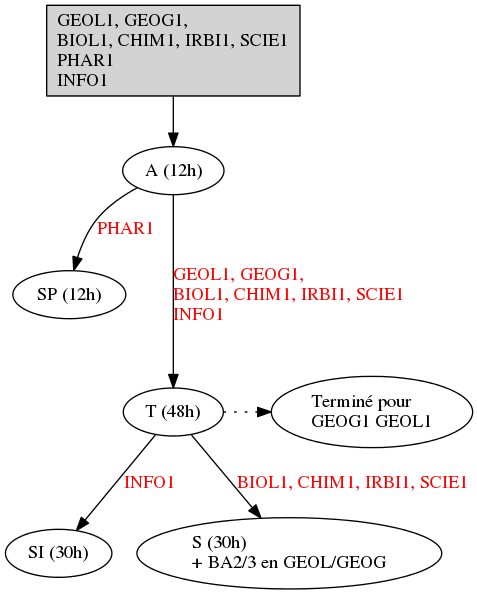
\includegraphics[width=\textwidth]{112-organisation-avec-anet-alt}
  \end{minipage}
\end{frame}
\begin{frame}{Examens}{À la grosse louche}
  \begin{description}
  \item[Réussite] Obtenir au moins 10/20.
  \item[Échec] Obtenir strictement moins que 10/20.
  \end{description}\pause

  Pour PHAR1 (24h de cours, tout au Q1)
  \begin{itemize}
  \item janvier (obligatoire !),
  \item juin (sur la même matière, obligatoire en cas d'échec en janvier),
  \item septembre (uniquement en cas d'échec en juin).\pause
    \par \small Uniquement en cas d'échec en juin ! (Art. 139 du décret \og Paysage\fg{}.)
  \end{itemize}\pause

  Pour tous les autres du BA1
  \begin{itemize}
  \item un test en novembre,
  \item une interro en janvier (obligatoire !),
  \item un examen en juin :
    \begin{itemize}
    \item Sur la partie du 2e quadri : obligatoire
    \item Sur la partie du 1er quadri : obligatoire si en échec en janvier
    \end{itemize}
  \item un examen en septembre (sur la matière de toute l'année)
    \par \small Uniquement en cas d'échec en juin ! (Art. 139 du décret \og Paysage\fg{}.)
  \end{itemize}
\end{frame}
\begin{frame} {Examens}{Durées et pondérations en janvier et juin}
  \begin{description}
  \item [PHAR1, 24h] Examen de 3h maximum.
    \begin{itemize}
    \item 8 points pour les 12 premières heures (avec N.R.)
    \item 12 points pour les 12 suivantes (avec Julien Federinov)
    \end{itemize}

  \item[GEOL1, GEOG1 : 60h] Examens de 3h en janvier, 1h30 (si Q1 non représenté) ou 4h (si Q1 représenté) en juin
    \begin{itemize}
    \item 16 points pour le Q1
    \item 4 points pour le Q2
    \end{itemize}
  \item[GEOL2 GEOG2 : 30h] le cours est au Q2. Un seul examen de 3h en juin.
  \item[BIOL1, SCIE1, CHIM1, IRBI1, INFO1] Examen de 3h en janvier, deux parties de 2h en juin.
    \begin{itemize}
    \item 10 points pour le Q1
    \item 10 points pour le Q2
    \end{itemize}
  \end{description}
\end{frame}
\begin{frame}{Examens}{Et le test de novembre ?}
  Pour ceux
  \begin{itemize}
  \item qui ont un test en novembre, \emph{et}
  \item qui réussissent mieux en novembre qu'en janvier.
  \end{itemize}
  Leur note de finale pour le Q1 est la moyenne pondérée~:
  \begin{itemize}
  \item pour un quart de celle de novembre, et
  \item pour trois-quarts de celle de janvier.
  \end{itemize}
\end{frame}
\begin{frame}{Examens}{Durées et pondérations en septembre}
  L'examen du mois de septembre est un examen unique couvrant \emph{toute la matière}. La durée est la même qu'en juin. La pondération des quadrimestres est identique à celle de juin.
\end{frame}
\begin{frame}
  \frametitle{Syllabus et exercices}
  \begin{itemize}[<+->]
  \item Le syllabus pour les modules \(A, T, S\) se trouve aux PUB (un fascicule par module), il sera également disponible sur l'Université Virtuelle.
  \item Le syllabus sera également, bientôt, disponible en version partagée.
  \item Les énoncés pour les séances d'exercices seront bientôt mis sur l'Université Virtuelle dans la soirée, aujourd'hui.
  \item Pour \emph{la première} séance d'exercices, des énoncés seront apportés par les assistants,
  \item pour les suivantes veuillez apporter les énoncés avec vous !
  \end{itemize}
\end{frame}

\section{Notions de mathématiques}
\begin{frame}{Définitions et résultats}
  \begin{definition}
    Une \Defn{définition} est une manière d'attribuer un mot ou une notation à un concept.
  \end{definition}

  \begin{example}
    La description du mot \og définition\fg{} ci-dessus peut-être vue comme une définition.
  \end{example}\pause

  \begin{example}Un exemple plus classique et plus \og mathématique\fg{} :
    \begin{definition}
      Un \Defn{carré} est un quadrilatère plane ayant tous ses angles égaux et tous ses côtés de même longueur.
    \end{definition}
  \end{example}\pause
\end{frame}
\begin{frame}%FIXME: intégrer au syllabus
  \begin{theorem}
    La longueur de la diagonale d'un carré vaut la longueur d'un de ses côtés multiplée par la racine carrée de \(2\).
  \end{theorem}
  \begin{proof}\pause
    La preuve, à l'aide du théorème de Pythagore, est laisée en exercice.
  \end{proof}
\end{frame}

\begin{frame}{Notation}
  Chaque notation est soit
  \begin{itemize}
  \item une notation bien connue (et utilisée sans précision)
  \item une notation ad-hoc (définie le temps d'un énoncé, d'un paragraphe, d'un cours, \dots).
  \end{itemize}
  \begin{example}
    Si \(x + 1 = 2\), alors \(x = 1\).\pause

    Si \(x^{2} = 4\), alors \(x = 2\) ou \(x = -2\).\pause

    On peut changer le sens de la variable d'une ligne à l'autre.
  \end{example}
  \begin{example}
    Pour un cercle de rayon \(R\) :

    \(\text{Aire} = \pi{R^2}\)

    \(\text{Périm} = 2 \pi{R}\)
  \end{example}
\end{frame}

\begin{frame}{Démonstration}
  \begin{definition}
    Démonstration : succession d'affirmations qui découlent les unes des autres par applications de règles logiques à des résultats déjà connus.
  \end{definition}
\end{frame}
\begin{frame}
  
  \begin{example}Définissons \og être divisible par\fg{} par \og le quotient est un entier\fg{}, et \og pair\fg{} par \og être divisible par \(2\)\fg{}. Nous pouvons alors affirmer : le carré de tout entier pair est divisble par \(4\).
    \begin{proof}[Preuve/Démonstration]
      Si \(p\) est un entier pair, cela veut dire qu'il est divisible par \(2\) (définition de \og pair\fg{}) ; dès lors \(p/2\) est un entier, notons-le \(q\).\\
      Nous avons donc \(p/2 = q\)\\
      Dès lors, \((p/2)^{2} = q^{2}\) (car appliquer la même opération à un objet donné amène au même résultat)\\
      Or \((p/2)^{2} = p^{2}/4\)\\
      De plus, \(q^{2}\) est encore un entier, car le produit de deux nombres entiers est un nombre entier\\
      Dès lors, \(p^{2}\) est divisible par \(4\).
    \end{proof}
  \end{example}
\end{frame}

\begin{frame}{Manipuler le vrai et le faux}
  \begin{definition}
    On s'intéresse à la valeur de vérité des affirmations : vrai ou faux ? C'est soit l'un, soit l'autre.
  \end{definition}

  \begin{example}
    Considérons les affirmations suivantes
    \begin{itemize}
    \item \og $x$ est positif\fg{} ;
    \item \og Si \(x\) est plus grand que \(1\) alors \(x\) est positif\fg{} ;
    \item \og Pour tout $x$ entier, $x$ est positif\fg{} ;
    \item \og Il existe $x$ entier tel que $x$ est positif\fg{} ;
    \end{itemize}
  \end{example}
\end{frame}
\begin{frame}
  \begin{example}
    Il se fait que :
    \begin{itemize}
    \item la première est vraie ou fausse selon la valeur de $x$,
    \item la seconde est vraie quelle que soit la valeur de \(x\),
    \item la troisième est fausse et
    \item la dernière est vraie.
    \end{itemize}
  \end{example}
\end{frame}

\begin{frame}
  \frametitle{Connecteurs logiques}
  En construisant les affirmations, nous utilisons des connecteurs logique : \og et\fg{} (noté \(\land\)), \og ou\fg{} (noté \(\lor\)), \og implique\fg{} (noté \(\ldonc\)), etc.

  \begin{example}
    S'il pleut ou s'il grèle, je prends mon parapluie.\pause

    \begin{itemize}
    \item Notons \(P\) l'affirmation \og Il pleut\fg{},
    \item Notons \(G\) l'affirmation \og Il grèle\fg{},
    \item Notons \(A\) l'affirmation \og Je prends mon parapluie\fg{}.
    \end{itemize}
    Alors on peut ré-écrire l'affirmation initiale sous forme symbolique :
    \begin{equation*}
      (P \lor G) \ldonc A
    \end{equation*}
  \end{example}
\end{frame}

\begin{frame}{Raisonnements}%FIXME: intégrer au syllabus
  La capacité à raisonner est indispensable.

  \begin{example}
    J'ai 3 paires de chaussettes différentes. Si je choisis au hasard sans regarder, combien dois-je prendre de chaussettes dans ma valise pour être totalement certain d'avoir au moins deux chaussettes d'une même paire ?
  \end{example}
\end{frame}

\begin{frame}{Raisonnements}{L'énigme}
  \begin{quote}
    Il y a cinq maisons de cinq couleurs différentes.

    Dans chacune de ces maisons, vit une personne de nationalité différente.

    Chacune de ces personnes boit une boisson différente, fume un cigare différent et a un animal domestique différent.
    \begin{itemize}
    \item L'Anglais vit dans la maison rouge.
    \item Le Suédois a des chiens.
    \item Le Danois boit du thé.
    \item La maison verte est à gauche de la maison blanche.
    \item Le propriétaire de la maison verte boit du café.
    \item \(\vdots\)
    \item (l'énoncé complet se trouve dans le syllabus et sur Internet)
    \end{itemize}
    Question : qui a le poisson ?
  \end{quote}
\end{frame}

\begin{frame}{Démonstration par l'absurde}
  \begin{question}
    Existe-t-il un nombre qui, multiplé par \(0\), vaut \(1\) ?
  \end{question}\pause

\begin{example}
  Supposons, par l'absurde, supposons qu'un tel nombre \(a\) existe.

  Alors \(a0 = 0\).

  Dès lors nous aurions \(0 = 1\), qui est une contradiction.
\end{example}
\end{frame}

\begin{frame}
  \begin{question}
    Existe-t-il un nombre strictement positif qui soit plus petit que tous les autres nombres strictement positifs ?
  \end{question}
\end{frame}

\begin{frame}{Contraposée}
  \begin{example}
    Les affirmations \og S'il pleut je prends mon parapluie\fg{} et \og Si je ne prends pas mon parapluie, c'est qu'il ne pleut pas\fg{} sont parfaitement équivalentes du point de vue des valeurs de vérité. On peut également facilement passer de l'une à l'autre par un raisonnement par l'absurde.
  \end{example}

\begin{example}
  \og Si \(x\) est divisible par \(6\), alors \(x\) est pair\fg{} est équivalente à \og Si \(x\) n'est pas pair, alors \(x\) n'est pas divisible par \(6\)\fg{}.
\end{example}
\end{frame}

\begin{frame}{Démonstration par récurrence / induction}{Principe}
  Supposons que nous voulions démontrer une proposition \(p(n)\) pour tout entier naturel \(n\) (c'est-à-dire \(n = 0, 1, 2, \ldots\)).

  Si nous pouvons prouver~:
  \begin{itemize}
  \item \(p(0)\) (\og le pas initial\fg{}), et
  \item \(\forall k\in \NN, p(k) \ldonc p(k+1)\) (\og l'étape d'induction\fg{}),
  \end{itemize}
  alors le principe d'induction affirme que \(\forall n\in \NN, p(n)\).
\end{frame}
\begin{frame}{Démonstration par récurrence / induction}{Exemple}
  Montrons par récurrence que la somme des entiers de \(0\) à \(n\) vaut \(\frac{n(n+1)}{2}\). C'est notre affirmation \(p(n)\).

  L'affirmation \(p(0)\) est : \og La somme des entiers de \(0\) à \(0\) vaut \(0\).\fg{} \pause

  Ceci est clair. Le pas initial est donc prouvé.\pause
\end{frame}
\begin{frame}{Démonstration par récurrence / induction}{Exemple}
  Pour l'étape d'induction, fixons un nombre \(k\) quelconque, et supposons \(p(k)\), c'est-à dire supposons\pause
  \begin{equation*}
    0 + 1 + \cdots + k = \frac{k(k+1)}{2}.
  \end{equation*}\pause
  Nous voulons montrer \(p(k+1)\), c'est-à-dire~:
  \begin{equation*}
    0 + 1 + \cdots + (k+1) = \frac{(k+1)(k+2)}{2}.
  \end{equation*}\pause
  Or la somme du membre de gauche \og passe\fg{} par \(k\), c'est-à-dire qu'on peut l'écrire sous la forme
  \begin{equation*}
    \underbrace{0 + 1 + \cdots + k}_{= \frac{k(k+1)}{2}} + (k+1) = \frac{k(k+1)}{2} + (k+1)
  \end{equation*}\pause
\end{frame}
\begin{frame}{Démonstration par récurrence / induction}{Exemple}
  En mettant alors au même dénominateur, nous obtenons
  \begin{equation*}
    \frac{k(k+1)}{2} + (k+1) = \frac{k(k+1)+2(k+1)}{2}
  \end{equation*}\pause
  et, en mettant \(k+1\) en évidence, nous avons~:
  \begin{equation*}
    \frac{k(k+1)+2(k+1)}{2} = 
    \frac{(k+2)(k+1)}{2}
  \end{equation*}\pause
  Mettant maintenant bout à bout nos dernières égalités, nous avons obtenu~:
  \begin{equation*}
    0 + 1 + \cdots + (k+1) = \frac{(k+1)(k+2)}{2}
  \end{equation*}
  ce que nous voulions démontrer !\pause

  Par le principe d'induction, l'égalité \(p(n)\) est donc vraie pour tout entier \(n\).
\end{frame}

\begin{frame}{Modélisation}
  Pour beaucoup, les mathématiques seront un outil pour étudier une certaine réalité.

  La réalité étant bien généralement trop complexe, il faudra la simplifier.\pause

  Le passage d'une réalité complexe à une vision mathématisée, moins complexe, est la \Defn{modélisation} du problème.\pause

\begin{example}
  \og On lance une pièce de monnaie.\fg{} Il faut d'abord définir le problème :
  \begin{itemize}
  \item La trajectoire de la pièce ?
  \item À la manière dont elle tourne ?
  \item Au déplacement d'air qu'elle provoque ?
  \item Aux processus qui font qu'on est capable ou pas de ratrapper la pièce avant qu'elle retombe ?
  \item Ou, simplement, au résultat \og pile\fg{} ou \og face\fg{} obtenu ?
  \end{itemize}
\end{example}
\end{frame}

\section{Les nombres}
\begin{frame}{Une classification des nombres}
  Si on note \(\RR\) l'ensemble des nombres dits \og réels\fg{}, on a des inclusions~:
  \begin{equation*}
    \NN \subset \ZZ \subset  \QQ \subset \RR
  \end{equation*}
  où
  \begin{itemize}
  \item \(\NN = \set{0, 1, 2, 3, \ldots}\) est l'ensemble des (entiers) naturels.
  \item \(\ZZ = \set{0, 1, -1, 2,-2, 3,-3, \ldots}\) est l'ensemble des entiers (relatifs).
  \item \(\QQ\) est l'ensemble des rationnels (nombres qui s'écrivent comme fraction d'entiers).
  \end{itemize}\pause
  Les nombres réels qui ne sont pas dans \(\QQ\) sont dits \og irrationnels\fg{} (p.ex. \(\sqrt{3}\), \(\pi\), etc.)
\end{frame}

\begin{frame}%FIXME: intégrer au syllabus
  % ça s'y trouve partiellement
  \frametitle{Développement décimal}
  Le développement décimal d'un nombre est son écriture \og en chiffres\fg{}.

  Le développement décimal de \(x\) est \(y\)~:
  \begin{equation*}
    \begin{array}{cc}
      x & y \\\hline
      1 & 1 \\
      1/2 & 0.5\\
      1/3 & 0.333...3...\\
      1/11 & 0.090909...09...\\
      \pi & 3.14159...
    \end{array}
  \end{equation*}

  \begin{theorem}
    Un nombre est rationnel si et seulement si on développement décimal est périodique.
  \end{theorem}
\end{frame}
\begin{frame}{Précision, illusion de précision et arrondis}
  \begin{example}
    En roulant à vélo à \SI{20}{\km\per\hour} pendant 10 minutes, la distance parcourue est de 3.333...3...\si{\km}.
  \end{example}

  La présence des décimales laisse croire à une précision importante dans le calcul, alors qu'en réalité la vitesse utilisée (20 à l'heure) était probablement une approximation grossière.\pause

  \(\Rightarrow\) Dans les problèmes physique, on arrondit généralement les réponses.
\end{frame}

\section{Relations entre les nombres}
\subsection{Inégalités et notion d'ordre}
\label{sec:inegalites}
\begin{frame}
  Les nombres peuvent être comparés entre eux.
  \begin{definition}
    On dit que
    \begin{itemize}
    \item \og \(a\) est strictement inférieur à \(b\)\fg{}, noté \(a < b\), si \(a\) est plus petit et différent de \(b\) ;
    \item \og \(a\) est strictement supérieur à \(b\)\fg{}, noté \(a > b\), si \(a\) est plus grand et différent de \(b\) ;
    \item \og \(a\) est inférieur à \(b\)\fg{} (ou \og inférieur ou égal\fg{}), noté \(a \leq b\), si \(a\) est plus petit ou égal à \(b\) ;
    \item \og \(a\) est supérieur à \(b\)\fg{} (ou \og supérieur ou égal\fg{}), noté \(a \geq b\), si \(a\) est plus grand ou égal à \(b\).
    \end{itemize}
  \end{definition}
\end{frame}
\begin{frame}
  \begin{example}
    Les affirmations suivantes sont vraies~:
    \begin{itemize}
    \item \(2 \leq 3\)
    \item \(2 < 3\)
    \item \(-2 \leq 1\)
    \item \(-2 \leq -1\)
    \item \(2 \leq 2\)
    \item \(2 \geq 2\)
    \item \(5 > 3\)
    \end{itemize}
  \end{example}
\end{frame}
\begin{frame}
  
\begin{example}
  Mais celles-ci sont fausses~:
  \begin{itemize}
  \item \(2 \geq 3\)
  \item \(-2 \geq 1\)
  \item \(-2 \geq -1\)
  \item \(2 < 2\)
  \item \(2 > 2\)
  \item \(5 < 3\)
  \end{itemize}
\end{example}
\end{frame}

\begin{frame}
  \begin{remark*}
    L'inégalité \(2 \leq 2\) peut perturber, mais c'est l'usage en mathématique : \(\leq\) signifie \og plus petit ou égal\fg{}, donc en particulier puisque \(2 = 2\), on a forcément \(2 \leq 2\).
  \end{remark*}
\end{frame}

\begin{frame}
  Nous supposons les deux résultats suivant connu.
  \begin{property}% AXIOM
    Pour tous réels \(a,b,c\), nous avons :
    \begin{itemize}
    \item Si \(a \leq b\) et \(b \leq a\), alors \(a = b\)
    \item Si \(a \leq b\) et \(b \leq c\), alors \(a \leq c\) (propriété de transitivité).
    \end{itemize}
  \end{property}
  \begin{property}% AXIOM
    Soient \(a,b\) des nombres réels tels que \(a \leq b\). Alors pour tout réel \(c\) nous avons
    \begin{equation*}
      a + c \leq b + c.
    \end{equation*}
    De plus, si \(c \geq 0\), on a
    \begin{equation*}
      ac \leq bc
    \end{equation*}
  \end{property}
\end{frame}

\begin{frame}
  \begin{proposition}\label{prop:inegalites}
    Soient \(a,b,c,d\) des réels vérifiant \(a \leq b\) et \(c \leq d\). Alors
    \begin{equation*}
      a+c \leq b+d.
    \end{equation*}
    De plus, si \(0 \leq a\) et \(0 \leq c\), alors
    \begin{equation*}
      ac \leq bd.
    \end{equation*}
  \end{proposition}
  \begin{proof}
    Comme \(a \leq b\), alors \(a + c \leq b + c\) (résultat précédent). De même, comme \(c \leq d\), nous avons \(b + c \leq b + d\). Par transitivité, nous obtenons \(a + c \leq b + d\) comme annoncé.

    La preuve pour le produit (avec la condition supplémentaire) est laissée en exercice.
  \end{proof}
\end{frame}

\begin{frame}
  \begin{exercise}
    Faire la preuve de la seconde partie du résultat~\ref{prop:inegalites}.
  \end{exercise}
  \begin{exercise}
    Trouver des réels \(a,b,c,d\) tels que \(a \leq b\), \(c \leq d\) et \(ac > bd\).
  \end{exercise}
\end{frame}

\subsection{Intervalles}
\begin{frame}
  \begin{definition}
    Un \Defn{intervalle} s'entend comme un ensemble de nombres réels \og sans trou\fg{} (on parle d'ensemble \Defn{connexe}).
  \end{definition}

  \begin{example}
    \begin{itemize}
    \item Si on définit $\intercc{-2,\pi}$ comme l'ensemble des réels compris entre $-2$ et $\pi$, c'est un intervalle : il n'y a aucun trou entre ces deux nombres.
    \item L'ensemble des réels positifs (ou nuls), noté \(\RR^+\), est également un intervalle.
    \item L'ensemble des réels sauf \(0\), noté \(\RR_0\), n'est pas un intervalle car \(0\) manque : il y a un trou.
    \end{itemize}
  \end{example}
\end{frame}

\begin{frame}
  On peut classer les intervalles comme suit.
  \begin{property}
    Si \(a\) et \(b\) sont des nombres réels, on définit ces notations :
    \begin{itemize}
    \item $\intercc{a,b}$ désigne l'ensemble des réels de $a$ (compris) à $b$ (compris) ;
    \item $\interoc{a,b}$ désigne l'ensemble des réels de $a$ (non-compris) à $b$ (compris) ;
    \item $\interco{a,b}$ désigne l'ensemble des réels de $a$ (compris) à $b$ (non-compris) ;
    \item $\interoo{a,b}$ désigne l'ensemble des réels de $a$ (non-compris) à $b$ (non-compris) ;
    \item \(\interoo{-\infty,b}\) désigne l'ensemble des réels strictement inférieurs à \(b\) ;
    \item \(\interoc{-\infty,b}\) désigne l'ensemble des réels inférieurs ou égaux à \(b\) ;
    \item \(\interoo{a,\infty}\) désigne l'ensemble des réels strictement supérieurs à \(a\) ;
    \item \(\interco{a,\infty}\) désigne l'ensemble des réels supérieurs ou égaux à \(a\) ;
    \item \(\interoo{-\infty,\infty}\) désigne l'ensemble des réels, également noté \(\RR\).
    \end{itemize}
    % Dans les notations ci-dessus, \(a\) et \(-\infty\) sont la \Defn[borne!inférieure]{borne inférieure} des intervalles dans lesquels ils apparaissent, tandis que \(b\) et \(\infty\) sont la \Defn[borne!supérieure]{borne supérieure} des intervalles dans lesquels ils apparaissent.
  \end{property}
\end{frame}


\begin{frame}
  Un intervalle est généralement \og infini\fg{} car il contient une infinité de nombre, mais parfois il est néanmoins \og borné\fg{}

  \begin{example}
    \begin{itemize}
    \item L'intervalle \(\intercc{0,1}\) contient une infinité de nombres, puisqu'il contient notamment \(1\), \(\frac{1}{2}\), \(\frac{1}{3}\), \(\frac{1}{4}\), etc. Mais il est également borné, car aucun des nombres n'est inférieur à \(0\) ou supérieur à \(1\) (de par la définition de cet intervalle !).
    \item L'intervalle \(\intercc{4,4}\) contient un seul nombre : le nombre \(4\).
    \item L'intervalle \(\interoo{4,4}\) ne contient aucun nombre, car rien aucun nombre n'est à la fois strictement supérieur et strictement inférieur à \(4\).
    \end{itemize}
  \end{example}
\end{frame}

\begin{frame}
  Un ensemble \(A \subset \RR\) est \Defnemph{ouvert} si, de tout point de \(A\), on peut se déplacer un peu dans chaque direction tout en restant dans \(A\). \pause
  \begin{definition}
    Soit \(A \subset \RR\), un ensemble.
    \begin{itemize}
    \item L'\Defn{intérieur} de \(A\) est composé des points \(p \in \RR\) tels qu'il existe \(\epsilon > 0\) vérifiant \(\interoo{p-\epsilon,p+\epsilon}\subset A\). (En particulier \(p \in A\) !) On note \(\interior A\) l'intérieur de \(A\).%\notation{\interior}
    \item L'ensemble \(A\) est \Defn{ouvert} si \emph{pour tout} \(p \in A\) il existe \(\epsilon > 0\) tel que \(\interoo{p-\epsilon,p+\epsilon}\subset A\).
    \end{itemize}
  \end{definition}
\end{frame}
\begin{frame}
  Avant de donner une définition rigoureuse, voyons deux exemples :
  \begin{example}
    \begin{enumerate}
    \item L'ensemble des réels strictement positifs \(\RR_{0}^+\) est un ouvert : pour tout point de \(x > 0\), il est possible de s'éloigner un peu de \(x\) tout en restant strictement positif. Il suffit de s'éloigner d'une distance inférieure à \(x\).
    \item L'ensemble des réels positifs ou nuls \(\RR^+\) n'est \emph{pas} un ouvert : si on part de \(0\), il est impossible de se déplacer \og vers les négatifs\fg{} en restant dans \(\RR^+\). Quelle que soit la distance parcourue, on se retrouve hors de \(\RR^+\).
    \item L'ensemble \(\NN\) n'est \emph{pas} un ouvert de \(\RR\) : partant d'un entier naturel quelconque, il suffit de se déplacer un petit peu pour ne plus être entier ! Bien sûr, en se déplaçant plus longtemps on retombe sur des entiers, mais ça \og ne compte pas\fg{}. Pour le comprendre, il faut avoir la définition rigoureuse ci-dessous.
    \end{enumerate}
  \end{example}
\end{frame}

\begin{frame}
  \begin{definition}
    Soit \(A \subset \RR\), un ensemble.
    \begin{itemize}
    \item L'\Defn{adhérence} de \(A\) est composée des points \(p \in \RR\) tels que pour tout \(\epsilon > 0\), il existe \(a \in A\) avec \(\abs{a-p} < \epsilon\). On note \(\adh A\) l'adhérence de \(A\).
    \item L'ensemble \(A\) est \Defn{fermé} si tous les points qui adhèrent à \(A\) sont dans \(A\).
    \end{itemize}
  \end{definition}
  \begin{remark}
    Le mathématicien est facétieux : un ensemble ouvert peut également être fermé (mais c'est rare), et un ensemble qui n'est pas ouvert peut très bien ne pas être fermé (ça arrive souvent !).
  \end{remark}
\end{frame}

\begin{frame}
  \begin{proposition}
    Pour tout ensemble \(A\), nous avons \(\interior A \subset A \subset \adh A\).
  \end{proposition}
\end{frame}

\begin{frame}
  \begin{example}
    \begin{enumerate}
    \item Le nombre \(0\) est dans l'adhérence de \(\RR_{0}^+\) : il existe des nombres strictement positifs qui sont très proches de \(0\). Aussi proche qu'on veut. Notons que, comme \(0\) n'est pas lui-même strictement positif, cela implique que \(\RR_0^+\) n'est pas fermé.
    \item L'ensemble des réels positifs ou nuls \(\RR^+\) est fermé : aucun point hors de \(\RR^+\) n'est adhérent à \(\RR^+\).
    \item L'ensemble \(\NN\) est fermé.
    \item Soit \(A = \interoc{0,1}\). Le nombre \(0\) est adhérent à \(A\). Le nombre \(1\) n'est pas dans l'intérieur de \(A\). De ces deux affirmations, nous déduisons que \(A\) n'est ni fermé, ni ouvert.
    \end{enumerate}
  \end{example}
\end{frame}

% \begin{exercise}
%   Parmi les différentes sortes d'intervalle, certains sont ouverts et pas d'autres. L'auteur de ces notes est un grand distrait et a oublié lesquels sont ouverts, lesquels sont fermés (certains sont les deux, et d'autres aucun des deux !). Indiquez les bonnes réponses ci-dessous :
%   \begin{itemize}
%   \item $\intercc{a,b}$
%   \item $\interoc{a,b}$
%   \item $\interco{a,b}$
%   \item $\interoo{a,b}$
%   \item \(\interoo{-\infty,b}\)
%   \item \(\interoc{-\infty,b}\)
%   \item \(\interoo{a,\infty}\)
%   \item \(\interco{a,\infty}\)
%   \item \(\interco{-\infty,\infty}\)
%   \end{itemize}
%   (On suppose que \(a\) et \(b\) sont des réels vérifiant \(a < b\).)
% \end{exercise}

\subsection{Pourcentages}
\begin{frame}
  Un pourcentage est une façon commode de quantifier le rapport entre deux quantités.

\begin{example}
  \og 50\% des humains sont des femmes.\fg{} Ceci signifie que dans la population, la moitié sont des femmes. En effet, \(\frac{50}{100} = \frac{1}{2}\).
\end{example}
\pause

Le \og pourcent\fg{} décrit une proportion \og pour cent unités\fg{}. En d'autres termes, on décrit un nombre qui doit être divisé par cent.

\begin{example}
  \og Le taux de réussite des étudiants de bachelier de l'année passée était d'un tiers.\fg{} En d'autres termes, un étudiant sur trois avait réussi. Ceci est approximativement 33\% car
  \begin{equation*}
    \frac{1}{3} = \frac{\frac{1}{3}100}{100} = \frac{33.3\ldots3\ldots}{100} = 33.3\ldots3\ldots\%
  \end{equation*}
\end{example}
\end{frame}

\begin{frame}
  \begin{itemize}
  \item Le pourcentage est une information globale, et non individuelle.

\begin{example}
  Un taux de 33\% ne veut pas dire qu'en prenant trois étudiants au hasard, un seul réussira.
\end{example}
\pause
\item Le pourcentage n'est pas de la voyance.

\begin{example}
  Le taux de réussite peut très bien être différent cette année ! Il dépend de vous !
\end{example}
\end{itemize}
\end{frame}
\section{Manipulation et opération sur les nombres}
\begin{frame}
  \subsection{Sommes}
  Considérons les calculs suivants~:
  \begin{equation*}
    1 + 2 = 3, 1 + 2 + 3 = 6, 1 + 2 + 3 + 4 = 10, \ldots
  \end{equation*}
  Comment exprimer un calcul pour sommer les cent nombres de \(1\) jusqu'à \(100\) ? Où jusqu'à une valeur \(n\) quelconque ? Une solution classique est d'inventer une notation !

  Nous définissons un \Defn{symbole de sommation}% \notation{\sigma}
  comme suit~:
  \begin{definition}
    Si \(m\) et \(n\) sont des entiers, \(m \leq n\), et si \(a_{m}, a_{m+1}, \ldots, a_{n}\) sont des nombres, on définit :
    \begin{equation*}
      \sum_{k = m}^{n} a_{k} \pardef a_{m} + a_{m+1} + a_{m+2} + \cdots + a_{n-1} + a_{n}.
    \end{equation*}
  \end{definition}
\end{frame}

\begin{frame}
  \begin{example}La notion est très simple mais requiert quelques exemples. Il s'agit juste de donner une autre manière d'écrire les sommes.
    \begin{align*}
      \sum_{k= 1}^{100} k &= 1 + 2 + 3 + \ldots + 100\\
      \sum_{k= 1}^{100} k^{2} &= 1 + 4 + 9 + \ldots + 10000\\
      \sum_{k= 1}^{100} \frac{1}{k} &= \frac{1}{1} + \frac{1}{2} + \frac{1}{3} + \ldots + \frac{1}{100}\\
      \sum_{k= 1}^{100} 3 &= 3 + 3 + 3 + \cdots + 3 (= 300)\\
      \sum_{k= 5}^{10} (k-1) &= 4 + 5 + 6 + 7 + 8 + 9
    \end{align*}
  \end{example}
\end{frame}
\begin{frame}
  \begin{example}
    \begin{align*}
      \sum_{k= 5}^{5} (k-1) &= 4\\
      \frac{1}{100}\sum_{k= 1}^{100} k &= \frac{1 + 2 + 3 + \ldots + 100}{100}\\
      \sum_{k= 1}^{100} \frac{k}{100} &= \frac{1}{100} + \frac{2}{100} + \frac{3}{100} + \ldots + \frac{100}{100}\\
      (n+1) + \sum_{k=1}^{n} k &= (n+1) + (1 + 2 + 3 + \cdots + n) \\
                            &= 1 + 2 + 3 + \cdots + n + (n+1)\\
                            &= \sum_{k=1}^{n+1}.
    \end{align*}
  \end{example}
\end{frame}

\begin{frame}
  \begin{property}Le symbole somme vérifie les relations suivantes~:
    \begin{align*}
      \sum_{k = m}^{n} (a_{k}+b_{k}) &= \paren*{\sum_{k = m}^{n} a_{k}} + \paren*{\sum_{k = m}^{n} b_{k}}\\
      \sum_{k = m}^{n} \lambda a_{k} &= \lambda \sum_{k = m}^{n} a_{k}\\
      \sum_{k = m}^{n} a_{k} &= \sum_{k = m}^{n} a_{n+m-k}
    \end{align*}
  \end{property}
\end{frame}
\begin{frame}
  \begin{proof}
    Preuve de : \(\sum_{k = m}^{n} a_{k} = \sum_{k = m}^{n} a_{n+m-k}\) : Le membre de gauche est :
    \begin{equation*}
      \sum_{k = m}^{n} a_{k} = a_{m} + a_{m+1} + \cdots + a_{n}
    \end{equation*}
    et le membre de droite est
    \begin{align*}
      \sum_{k = m}^{n} a_{n+m-k} &= \begin{aligned}[t]
        a_{n+m-(m)} &+ a_{n+m-(m+1)} + a_{n+m-(m+2)} + \ldots\\
        &\ldots + a_{n+m-(n-1)} + a_{n+m-(n)}
      \end{aligned}\\
                                 &= a_{n} + a_{n-1} + a_{n-2} + \cdots + a_{m+1} + a_{m}
    \end{align*}
    Les deux sont donc égaux (l'un est simplement sommé dans un sens, l'autre l'est dans l'autre sens).
  \end{proof}
\end{frame}
%% Fin du premier cours
\course{2}
\begin{frame}{La guidance}{en mathématiques}
  \begin{description}[<+->]
  \item[Qu'est-ce ?] Pour poser vos questions de mathématiques, qu'elles soient en lien ou non avec ce cours-ci.
  \item[Quand ?] Tous les jours de 12h15 à 13h45, à partir de mercredi prochain.
  \item[Où ?] À la Plaine : salle d'étude du bâtiment A (à confirmer! Vérifiez sur GeHoL un peu avant d'y aller.)
  \item[Pour qui ?] Pour vous !
  \item[Par qui ?] Des étudiants en Master en Math ou des chargés d'exercices extérieurs à l'ULB.
  \item[En blocus ?] Un horaire adapté sera également confectionné durant le blocus, mais n'attendez pas pour poser vos questions.
  \item[Qui contacter ?] \url{gmath@ulb.ac.be} (N.B. : je lis cette adresse)
  \end{description}

\end{frame}
\begin{frame}{Examens}{Une remarque importante sur le déroulement}
  \begin{block}{Info importante concernant la calculatrice}
    La calculatrice ne sera pas autorisée à l'examen.
  \end{block}
\end{frame}
\begin{frame}
  \frametitle{Rappel}
  Nous avons défini le signe somme :
  \begin{equation*}
    \sum_{k = m}^{n} a_{k} \pardef a_{m} + a_{m+1} + a_{m+2} + \cdots + a_{n-1} + a_{n}.
  \end{equation*}

  \begin{example}
    Nous avions déjà prouvé par récurrence, mais avec d'autres notations :
    \begin{equation*}
      \sum_{k=1}^{n} k = \frac{n(n+1)}{2}
    \end{equation*}
  \end{example}
\end{frame}
\begin{frame}
  Autre preuve du même résultat.
  \begin{proof}
    Appliquons le résultat déjà prouvé :
    \begin{equation*}
      \sum_{k=1}^{n} k = \sum_{k=1}^{n} (n+1-k)
    \end{equation*}
    et calculons
    \begin{align*}
      2 \paren*{\sum_{k=1}^{n} k} &= (\sum_{k=1}^{n} k) + (\sum_{k=1}^{n} k) \\
                                  &= (\sum_{k=1}^{n} k) + (\sum_{k=1}^{n} (n+1-k)) \\
                                  &= \sum_{k=1}^{n} (k+(n+1-k)) \\
                                  &= \sum_{k=1}^{n} (n+1) &= n (n+1)
    \end{align*}
  \end{proof}
\end{frame}

\subsection{Moyenne arithmétique}
\begin{frame}{Moyenne}
  \begin{definition}
    La moyenne arithmétiques de \(n\) nombres \(x_{1}, \ldots, x_{n}\) est la quantité
    \begin{equation*}
      \mean{x} = \frac{\sum_{k=1}^{n} x_{k}}{n}
    \end{equation*}
  \end{definition}
  \pause
  \begin{example}
    Si un étudiant a suivi trois cours, et a obtenu les notes \(x_{1}\), \(x_{2}\) et \(x_{3}\), alors sa moyenne (arithmétique) est \(\frac{x_{1} + x_{2} + x_{3}}{3}\).
  \end{example}
  \begin{example}
    Si cinq étudiants ont suivi le cours de mathématiques, et ont eut des notes \(e_{1}, e_{2}, e_{3}, e_{4}, e_{5}\), alors on dira que la moyenne des notes pour ce cours est
    \begin{equation*}
      \frac{e_{1} + e_{2} + e_{3} + e_{4} + e_{5}}{5}.
    \end{equation*}
  \end{example}
\end{frame}

\begin{frame}
  \begin{property}
    La moyenne arithmétique d'une séquence de nombres est toujours plus petite que le plus grands de ces nombres, et plus grande que le plus petit de ces nombres.
  \end{property}
  \begin{proof}
    Considérons la moyenne \(\mean x\) de \(n\) nombres \(x_{1}, \ldots, x_{n}\). L'un de ces nombres, \og le plus petit\fg{}, est inférieur ou égal à tous les autres. Il a donc un certain indice, disons \(j\). De même, le plus grand a un certain indice disons \(J\). C'est-à-dire qu'on a \(x_{j} \leq x_{k} \leq x_{J}\) pour tout \(k\) entre \(1\) et \(n\). Dès lors~:
    \begin{equation*}
      x_{1} + x_{2} + \cdots + x_{n} \leq x_{J} + x_{J} + \cdots + x_{J} = n x_{J}
    \end{equation*}
    (ceci est une application répétée de la proposition~\ref{prop:inegalites}) dont on tire
    \begin{equation*}
      \mean{x} \leq x_{J}
    \end{equation*}
    c'est-à-dire : la moyenne d'une séquence de nombres est inférieure au plus grand de ces nombres.

    La preuve se termine similairement avec \(x_{j}\).
    % \begin{equation*}
    %   x_{1} + x_{2} + \cdots + x_{n} \geq x_{j} + x_{j} + \cdots + x_{j} = n x_{j}
    % \end{equation*}
    % d'où \(\mean{x} \geq x_{j}\), ce qui est le résultat annoncé.
  \end{proof}
\end{frame}
\subsection{Puissances}\label{sec-puissances}
\begin{frame}{Sur la notation des produits}
  \begin{block}{}
    Généralement le produit entre deux quantités se note en juxtaposant ces quantités.
  \end{block}

  \begin{example}
    Par exemple \(ab\) veut dire \og \(a\) fois \(b\)\fg{}, et \(3 x\) veut dire \og \(3\) fois \(x\)\fg{}.
  \end{example}\pause

  \begin{example}
    Si \(a = 3\) et \(b = 5\), écrire \(ab = 35\) est source de confusion !\pause
      
    Autre notation : \(3\cdot 5\) pour désigner le produit de \(3\) et de \(5\).

    Nous n'utilisons \emph{pas} la notation \(3\times 5\), pour éviter de confondre le symbole \(\times\) avec la variable \(x\).
  \end{example}
\end{frame}

\begin{frame}{Puissances}{Remarques générales}
  \begin{equation*}
    x^{b} = \underbrace{x \cdot x \cdot \cdots \cdot x}_{b\text{ fois}}.
  \end{equation*}

  Cas particulier: \(x^{0} = 1\).\pause

  \begin{property}Pour tous réels \(x,y\) et pour tous naturels \(a,b\), nous avons
    \begin{align}
      x^{a} y^{a} &= (xy)^{a}  & x^{a} x^{b} &= x^{a+b}\\
      (x^{a})^{b} &= x^{ab} & \frac{x^{a}}{x^{b}} &= x^{a-b}
    \end{align}
  \end{property}
\end{frame}
\begin{frame}{Combinatoire}{Questions de comptage}
  % FIXME: intégrer au syllabus -- les exemples sont neufs.
  \begin{question}
    Combien de séquences de 5 lettres peut-on réaliser avec les lettre A, C, G et T ?%FIXME: vérifier
  \end{question}
  \begin{answer}%\pause
    \begin{center}
    \begin{math}
      4 \times 4 \times 4 \times 4 \times 4 \pause = 4^5 = 1024
    \end{math}
  \end{center}
  \end{answer}\pause

  \begin{question}
    Combien de séquences de 8 chiffres peut-on réaliser avec les chiffres 0 et 1 ?
  \end{question}
  \begin{answer}\pause
    \begin{equation*}
      2^8 = 256
    \end{equation*}
  \end{answer}
\end{frame}
\begin{frame}
  % FIXME: intégrer au syllabus -- les exemples sont neufs.
  \addtobeamertemplate{block begin}{\vspace*{-3pt}}{}
  \frametitle{Factorielle}
  \begin{question}
    Combien de séquences de 4 lettres peut-on réaliser avec les lettres A, C, G et T en utilisant une seule fois chaque lettre ?
  \end{question}
  \begin{answer}
    \begin{equation*}
      4 \times 3 \times 2 \times 1 = 24
    \end{equation*}
  \end{answer}\pause
  \begin{definition}
    La factorielle d'un naturel \(n > 0\) est définie par :
    \begin{equation*}
      n! \pardef n (n-1)(n-2) \cdots 4 \cdot 3 \cdot 2 \cdot 1
    \end{equation*}
    Pour \(n = 0\), on définit \(0! = 1\).
  \end{definition}\pause
  \begin{example}
    \begin{align*}
      0! &= 1 & 1! &= 1 & 2! &= 2 & 3! &= 6 & 4! &= 24 & 5! &= 120 & \cdots
    \end{align*}
  \end{example}
\end{frame}
\begin{frame}
  \begin{proposition}Pour tout \(n > 0\),
    \begin{equation*}
      n! = n (n-1)!
    \end{equation*}
  \end{proposition}
  \begin{proof}\pause
    \begin{align*}
      n! &\pardef n (n-1)(n-2) \cdots 4 \cdot 3 \cdot 2 \cdot 1\\
         &= n [(n-1)(n-2) \cdots 4 \cdot 3 \cdot 2 \cdot 1]\\
         &= n (n-1)!
    \end{align*}
  \end{proof}
\end{frame}
\begin{frame}  % FIXME: intégrer au syllabus -- les exemples sont neufs.
  \begin{question}
    Combien séquences de 2 lettres (différentes) peut-on former avec \(A, C, T, G\) ?
  \end{question}
  \begin{answer}
    \(4 \times 3 = 12.\)
  \end{answer}
  \begin{question}
    Combien de séquences de \(k\) lettres (différentes) peut-on former avec \(n\) lettres (différentes) données ?
  \end{question}
  \begin{answer}
    \begin{equation*}
      n (n-1) (n-2) \cdots (n-(k-1)) \pause = \frac{n!}{(n-k)!}
    \end{equation*}
  \end{answer}
\end{frame}
\begin{frame}  % FIXME: intégrer au syllabus -- les exemples sont neufs.
  \begin{question}
    Combien de \og tas\fg{} de \(k\) lettres (différentes) peut-on former avec \(n\) lettres (différentes) données ?
  \end{question}
  En d'autres termes : presque la même question qu'avant, mais en oubliant l'ordre des lettres !
  \begin{answer}\pause
    \begin{equation*}
      \frac{n!}{(n-k)!\alert{k!}}
    \end{equation*}
  \end{answer}
  \begin{definition}
    Pour \(0 \leq k \leq n\), on définit le coefficient binomial :
    \begin{equation*}
      \binom{n}{k} \pardef \frac{n!}{(n-k)!k!}
    \end{equation*}
  \end{definition}
\end{frame}
\begin{frame}% FIXME: intégrer au syllabus
  \frametitle{Propriétés des coefficients binomiaux}
  \begin{proposition}Pour tout naturel \(n\), pour tout naturel \(k \geq 1\) :
  \begin{equation*}
    \binom{n+1}{k} = \binom{n}{k} + \binom{n}{k-1}
  \end{equation*}
\end{proposition}
\begin{proof}
  \begin{align*}
    \frac{n!}{(n-k)!k!}& + \frac{n!}{(n-(k-1))!(k-1)!}\\
    &= \frac{n!\alert{(n-k+1)}}{(n-k)!k!\alert{(n-k+1)}} + \frac{n! \alert{k}}{(n-k+1)!\alert{k} (k-1)!}\\
    &= \frac{n!(n-k+1) + n! k}{k!(n-k+1)!} = \frac{n!(n\alert{-k}+1 \alert{+ k})}{(n+1-k)!k!} = \binom{n+1}{k}
  \end{align*}
\end{proof}
\end{frame}
\begin{frame}% FIXME: intégrer au syllabus
  \frametitle{Triangle de Pascal}
  \fbox{\includegraphics[width=0.45\linewidth]{pascal}} % triangle rectangle
  \pause
  \fbox{\includegraphics[width=0.45\linewidth]{pascal2}} % triangle isocèle
\end{frame}
\begin{frame}% FIXME: intégrer au syllabus
  \begin{question}
  De combien de façons peut-on choisir \(k\) objects distincts parmis \(n\) objects distincts, sans prendre en compte leur ordre.
\end{question}
\begin{answer}\pause
  \begin{equation*}
  \binom{n}{k} \pause = \binom{n}{n-k}
\end{equation*}
\end{answer}\pause
  \begin{example}
    \begin{align*}
      (x+y)^2 &= (x+y)(x+y) = xx + xy + yx + yy = x^{2} + 2 xy + y^{2}\\
      (x+y)^3 &= (x+y)(x+y)(x+y)\\
              &= x(xx + xy + yx + yy) + y(xx + xy + yx + yy)\\
              &= x^{3} + 3 x^{2}y + 3 xy^{2} + y^{3}
    \end{align*}
  \end{example}
\end{frame}
\begin{frame}% FIXME: intégrer au syllabus
  \begin{proposition}[Binôme de Newton]
    \begin{align*}
      (x+y)^{n} &= (x+y)(x+y)\cdots(x+y)\\
                &=   \sum_{k=0}^{n} \binom{n}{k} x^{k} y^{n-k}
    \end{align*}
  \end{proposition}
  \begin{proof}
    Par récurrence.
  \end{proof}
\end{frame}

\subsection{Valeur absolue}
\begin{frame}
  La valeur absolue de \(x\), notée \(\abs{x}\), est définie par :
  \begin{equation*}
    \abs{x} \pardef \begin{cases}
      x &\textrm{si } x \geq 0\\
      -x & \textrm{si } x < 0 
    \end{cases}
  \end{equation*}

  \begin{example}
    \begin{itemize}
    \item \(\abs{5} = 5\) car \(5\) est positif, donc on est dans le premier cas.
    \item \(\abs{-5} = -(-5) = 5\) car \(-5\) est négatif, donc on est dans le second cas.
    \item \(0\) n'est pas spécial : \(\abs{0}= 0\) (premier cas).
    \end{itemize}
  \end{example}\pause
  \begin{remark}
    Si \(x,y\) sont des réels, alors \(\abs{x-y}\) s'interpète comme la distance entre \(x\) et \(y\).
  \end{remark}
\end{frame}

\begin{frame}% FIXME: intégrer au syllabus (la preuve n'y est pas)
  \begin{proposition}
    Pour tous \(x,y\), nous avons
    \begin{align*}
      \abs{x} &= \abs{-x} &  \abs{x-y} &= \abs{y-x} 
    \end{align*}
  \end{proposition}
\begin{proof}
  Pour la première égalité, on distingue trois cas :
  \begin{itemize}
  \item Si \(x=0\) est nul, alors \(-x = 0\),
  \item Si \(x>0\), alors \(-x < 0\) donc \(x = -(-x)\),
  \item Si \(x<0\), alors \(-x > 0\) donc \(-x = -x\).
  \end{itemize}
  Pour la seconde égalité, notons simplement que \(x-y = -(y-x)\).
\end{proof}
\end{frame}

\subsection{Écriture scientifique}
\begin{frame}
  \begin{example}Masse de Jupiter : \SI{1898600000000000000000000000}{\kg}. Problèmes :
    \begin{itemize}
    \item Même en tonne, on n'enlève que trois zéros.\pause
    \item Masse au kilogramme près ?!
    \end{itemize}
  \end{example}\pause

\begin{answer}
  On utilise la \Defn{notation scientifique} : \(m 10^{q}\).
\end{answer}

\begin{example}
  Voici les masses de quelques planètes de notre système solaire
  \begin{center}
    \begin{tabular}{ln{1}{4}|ln{1}{4}}
      \multicolumn{1}{l}{Planète} & \multicolumn{1}{r}{Masse (kg)}  % &    Planète & \multicolumn{1}{r}{Masse (kg)}
      \\ \toprule
      Jupiter &1.8986E27&Uranus &8.6832E25\\
      Saturne &5.6846E26&Terre &5.9736E24\\
      Neptune &1.0243E26&Vénus &4.8685E24\\
      % Mars &6.4185E23\\
      % Mercure &3.302E23\\
    \end{tabular}
  \end{center}
\end{example}
\end{frame}

\subsection{Racines}\label{sec-racines}
\begin{frame}
  Regardons un nombre \(x\), et considérons \(x^{2}\). Quelques valeurs~:
  \begin{equation*}
    \begin{array}{S[table-format=2.2]S[table-format=3.4]}
      x & x^{2}\\ \toprule
      0 & 0\\
      0.10 & 0.01\\
      0.50 & 0.25\\
      0.90 & 0.81\\
      0.99 & 0.9801\\
      1 & 1\\
      1.1 & 1.21\\
      1.5 & 2.25\\
      2 & 4\\
      10 & 100\\
      \bottomrule
    \end{array}
  \end{equation*}\pause
\begin{definition}Si \(t\) est un réel positif ou nul, sa \Defn{racine carrée}, notée \(\sqrt{t}\), est l'unique réel positif ou nul dont le carré vaut \(t\).
\end{definition}
\end{frame}
\begin{frame}
  \begin{remark}
    Si \(t\) est strictement positif, alors il existe exactement \emph{deux} nombres dont le carré vaut \(t\) : \(\sqrt{t}\) et \(-\sqrt{t}\).

    Le premier est positif, le second est négatif.
  \end{remark}\pause
  On peut sans problème étendre ces raisonnements à \(x^{3}\), \(x^{4}\), etc.
  \begin{definition}
    Si \(t\) est un réel positif ou nul, sa \Defn{racine $n$\ieme{}}, notée \(\sqrt[n]{t}\), est l'unique réel positif ou nul dont la puissance \(n\)\ieme{} vaut \(t\).
  \end{definition}
\end{frame}

\begin{frame}{Puissances et racines}
  \begin{example}
    La notation \(x^{1/3}\) a-t-elle du sens ? \pause
    Supposons que les règles précédentes restent valables, alors
    \begin{equation*}
      \paren{x^{1/3}}^{3} = x^{3/3} = x^{1} = x
    \end{equation*}\pause
    Dès lors, \(x^{1/3}\) doit être la racine cubique de \(x\) !
    \begin{equation*}
      x^{1/3} = \sqrt[3]{x}
    \end{equation*}
  \end{example}\pause
  \begin{definition}
    Si \(p\) et \(q\) sont naturels, on définit \(x^{p/q} \pardef (\sqrt[q]{x})^{p}\).
  \end{definition}
  \begin{remark}
    \begin{itemize}
    \item Cela coïncide avec la définition usuelle dès que \(p/q\) est un naturel.
    \item On peut définir \(x^{r}\) pour tout réel \(r\) dès que \(x > 0\).
    \end{itemize}
  \end{remark}
\end{frame}
\begin{frame}
  \begin{property}%AXIOM
    \label{resultat-puissances}
    Pour tous réels strictement positifs \(x,y\), et pour tous réels \(a,b\), nous avons
    \begin{align}
      x^{a} &> 0\\
      x^{a} y^{a} &= (xy)^{a}  & x^{a} x^{b} &= x^{a+b}\\
      (x^{a})^{b} &= x^{ab} & \frac{x^{a}}{x^{b}} &= x^{a-b}
    \end{align}
  \end{property}
\end{frame}

\section{Fonctions}
\begin{frame}
\begin{definition}
Se donner une \Defn{fonction} $f$ s'est se donner :
\begin{itemize}
\item un \Defn{ensemble de départ} $A$,
\item un \Defn{ensemble d'arrivée} $B$ et
\item une règle permettant d'associer à chaque élément $x$ de $A$ un unique élément de $B$ noté \(f(x)\).
\end{itemize}

\begin{itemize}
\item \(f(x)\) est l'\Defn{image} de $x$ par $f$.
\item On dit aussi que \(x\) est un \Defn{antécédent} de \(f(x)\).
\end{itemize}

La notation usuelle pour une fonction $f$ de $A$ dans $B$ est
\begin{equation*}
  f : A \to B : x \mapsto f(x)
\end{equation*}
\end{definition}
\end{frame}

\begin{frame}
\begin{example}Voici quelques exemples de fonctions :
  \begin{itemize}[<+->]
  \item Une fonction associant à chaque réel son carré
    \begin{equation*}
      g : \RR \to \RR : x \mapsto x^2 ;
    \end{equation*}
  \item la fonction valeur absolue
    \begin{equation*}
      h : \RR \to \RR : x \mapsto |x| ;
    \end{equation*}
  \item la fonction \Defn{plancher}
    \begin{equation*}
      i : \RR \to \ZZ : x \mapsto \lfloor x \rfloor
    \end{equation*}
    où $\lfloor x \rfloor$ est défini comme le plus grand entier $k$ tel que $k \leqslant x$;
  \end{itemize}
\end{example}
\end{frame}

\begin{frame}
  \begin{example}
    \begin{itemize}[<+->]
    \item la \Defn[fonction!caractéristique]{fonction caractéristique} de l'ensemble \(\QQ \subset \RR\)
      \begin{equation*}
        j : \RR \to \{0,1\} : x \mapsto 
        \begin{cases}
          1 &\text{si } x \in \QQ\\
          0 &\text{si } x \in \RR \setminus \QQ
        \end{cases}
      \end{equation*}
    \end{itemize}
  \end{example}
\end{frame}
\begin{frame}
  Toutes les fonctions ne concernent pas forcément des nombres.
  \begin{example}
    Soit \(A\) l'ensemble des étudiants à l'ULB, soit \(B\) l'ensemble des nombres naturels. On associe, à chaque étudiant, son numéro matricule. Chaque étudiant à l'ULB possède un tel numéro matricule, cela définit donc une fonction !
  \end{example}\pause
  \begin{example}La notation
    \begin{equation*}
      f : \RR \to \RR : x \mapsto \frac{1}{x}
    \end{equation*}
    ne définit \emph{pas} une fonction au sens précédent, car l'image de \(0\) n'a pas été définie. Par contre,
    \begin{equation*}
      g : \RR \to \RR : x \mapsto
      \begin{cases*}
        \frac{1}{x} & si \(x \neq 0\)\\
        0 & sinon.
      \end{cases*}
    \end{equation*}
    définit correctement une fonction.
  \end{example}
\end{frame}

\begin{frame}
  \begin{exercise}
    Comment choisir le domaine \(A \subset \RR\) pour que
    \begin{equation*}
      f : A \to \RR : x \mapsto \frac{1}{x^{2}-1}
    \end{equation*}
    définisse une fonction ?

    \begin{answer}
    N'importe quel \(A\) ne contenant ni \(1\) ni \(-1\) convient. Généralement, nous prenons \og le plus grand possible\fg{}, c'est-à-dire \(A = \RR\setminus\set{-1,1}\).
  \end{answer}


    %% FIXMEs: on peut le représenter comme suit:

    %% dans ce cas le graphe est: ...

    %% mais on pourrait aussi choisir par exemple \interoo{-1,1}, représenté comme suit:

    %% dans ce cas le graphe est: ...
  \end{exercise}\pause
  \begin{remark*}
    La règle qui donne $f(x)$ est souvent une simple formule (également appelée \Defn{expression algébrique}) contenant la variable~$x$. Parfois la recette est plus complexe, et parfois il n'y a aucune formule.
  \end{remark*}
\end{frame}

\begin{frame}{Coordonnées cartésiennes}
  \begin{definition}
    Un {repère cartésien} est la donnée de deux axes sécants, et d'une unité sur chaque axe. L'intersection des axes est appelée l'origine.

    Les coordonnées cartésiennes d'un point \(P\) du plan sont alors obtenues en projetant ce point sur chacun des axes, et en repérant la projection par rapport à l'unité.
  \end{definition}
  
  \begin{center}
    \includegraphics[height=4cm]{coordcart}
  \end{center}
\end{frame}

\begin{frame}{Graphe de fonction}
  Le graphe d'une fonction \(f\) est l'ensemble des couples \((x,f(x))\) \pause et on peut parfois le dessiner !
  \begin{center}
  \begin{tikzpicture}[xscale=2,yscale=1] %% Warning : bad practice
    %% inside (modif of xscale to kill the
    %% global effect)
    \draw (0,0) node [below left] {$0$};%
    \foreach \y in {1, ..., 4} \draw[xscale=.5] (3pt,\y) -- (-3pt,\y)
    node [left] {$\y$};%
    \foreach \x in {-2, -1, 1, 2} \draw (\x,-3pt) node [below] {$\x$} --
    (\x,3pt);%
    \draw [->] (0,-.2) -- (0,5) node [above left] {$y$};%
    \draw [->] (-2.2,0) -- (3,0) node [below right] {$x$};%

    % \draw[xscale=.5,ultra thick] (0,0) [fill] circle (2pt) -- (0,4)
    % circle (2pt);%
    \draw (0,0) parabola[bend at start] +(2,4) node
    [right] {$y = x^2$};
    \draw (0,0) parabola[bend at start] +(-2,4) node
    [right] {$y = x^2$};
    \draw [dashed] (1.5,0) -- (1.5,2.25) -- (0,2.25);
  \end{tikzpicture}
\end{center}
\end{frame}

\begin{frame}
  \begin{definition}
    Un repère est orthonormé si les axes sont perpendiculaires et les unités ont même longueur.
  \end{definition}\pause
  \begin{remark}
    En général, on prend un premier axe qui est \og horizontal\fg{}, et le second qui est vertical sur la feuille.

    Lorsque je mentionnerai le graphe d'une fonction, je ferai toujours l'hypothèse d'un repère orthonormé disposé de cette manière !
  \end{remark}
\end{frame}

\begin{frame}
  \begin{definition}
    Une fonction $f \colon A \to B$, avec $A \subset \RR$ et $B \subset \RR$ est~:
    \begin{itemize}
    \item \Defn{paire} si et seulement si pour tout $x$ de $A$, on a $-x \in A$ et $f(x) = f(-x)$.
    \item \Defn{impaire} si et seulement si pour tout $x$ de $A$, on a $-x \in A$ et $f(-x) = -f(x)$.
    \end{itemize}
  \end{definition}
  \begin{proposition}
    Une fonction est paire \(\iff\) son graphe est symétrique par rapport à l'axe vertical du repère.

    Une fonction est impaire \(\iff\) son graphe est symétrique par rapport à l'origine du repère.
  \end{proposition}
\end{frame}

\begin{frame}
  Soit $f : A \to B$ une fonction.
  \begin{itemize}
  \item $f$ est \Defn{surjective} si tout élément de $B$ est l'image d'au moins un élément de $A$ ;
  \item $f$ est \Defn{injective} si deux éléments distincts de $A$ ont des images distinctes ;
  \item $f$ est \Defn{bijective} si $f$ est à la fois injective et surjective.
  \end{itemize}\pause

  \begin{remark}
    Une fonction est injective si et seulement si toute droite horizontale coupe son graphe en \emph{maximum} un point !
  \end{remark}

  \begin{example}
    La fonction \(f : \RR \to \RR : x \mapsto x^{2}\)\pause n'est pas injective \pause ni surjective.\pause

    La fonction \(f : \RR^{+} \to \RR : x \mapsto x^{2}\)\pause est injective\pause, mais pas surjective.\pause

    La fonction \(f : \RR \to \RR : x \mapsto x^{3}\)\pause est injective \pause et surjective \pause donc bijective.
  \end{example}
\end{frame}

\begin{frame}
  Soit \(f : A \to B\) une fonction. L'ensemble image de \(f\), noté \(\im f\) ou \(f(A)\), est l'ensemble \(\set{f(x) \telque x \in A}\).

  L'ensemble image de la fonction
  \begin{itemize}
  \item \(f : \RR \to \RR : x \mapsto x^{2}\) est \(\RR^+\)\pause
  \item \(f : \RR \to \RR : x \mapsto x^{3}\) est \(\RR\)
  \end{itemize}
\end{frame}

\begin{frame}{Composées}
  \begin{definition}
    Si \(f : A \to B\) et \(g : C \to D\), avec \(\im f \subset \dom g\),\pause

    alors on peut former la \Defn{composée} \(g \circ f : A \to D : x \mapsto g(f(x))\).
  \end{definition}

  \begin{remark}
    Attention à l'ordre des opérations : \(g \circ f\) se lit \og \(g\) rond \(f\)\fg{},\pause mais à \(x\) l'on applique d'abord \(f\) puis \(g\).
  \end{remark}
\end{frame}
\course{3}

% \begin{frame}{Fonction identité}
%   \begin{definition}
%     Si \(A\) est un ensemble, la fonction \(A \to A : x \mapsto x\) est appelée l'\Defn{identité} sur \(A\)

%     On la note souvent \(\Id_A\), de sorte que \(\Id_A(x) = x\) pour tout \(x \in A\).
%   \end{definition}
% \end{frame}

\begin{frame}{Remarque importante}
  \begin{center}
    L'Université Virtuelle étant un peu lente, l'ensemble des documents se trouve également à l'adresse \url{http://homepages.ulb.ac.be/~nrichard/Math-F-112} sans que ce soit indiqué sur l'UV :
    \begin{itemize}[<+->]
    \item énoncés d'exercices
    \item liste des exercices sélectionnés
    \item syllabus (également disponible aux PUB) en PDF
    \item les slides (version couleur et version sans couleur)
    \end{itemize}
  \end{center}
\end{frame}

\begin{frame}{Antécédent}
  \begin{block}{Rappel}
    Si $x$, élément de $A$, vérifie $f(x)=y$, on dit que $x$ est un \Defn{antécédent} de $y$ (pour la fonction $f$). \pause

    Un élément $y$ de $B$ peut très bien avoir plusieurs antécédents ou n'en avoir aucun.
  \end{block}

  \begin{example}
    Les antécédents de $4$ par la fonction $f : \RR \vers \RR : x \mapsto x^2$ sont $-2$ et $2$. \pause

    L'unique antécédent de $0$ est $0$.\pause

    Par contre $-4$ n'a aucun antécédent pour cette fonction.
  \end{example}
\end{frame}

\begin{frame}
Le graphe de $[0,2] \to \RR : x \mapsto x^2$  et son ensemble image : \([0,4]\)
\begin{center}
  \begin{tikzpicture}[xscale=2,yscale=1] %% Warning : bad practice
    %% inside (modif of xscale to kill the
    %% global effect)
    \draw (0,0) node [below left] {$0$};%
    \foreach \y in {1, ..., 5} \draw[xscale=.5] (3pt,\y) -- (-3pt,\y) node [left] {$\y$};%
    \foreach \x in {1, 2} \draw (\x,-3pt) node [below] {$\x$} -- (\x,3pt);%
    \draw [->] (0,-.2) -- (0,6) node [above left] {$y$};%
    \draw [->] (-.2,0) -- (3,0) node [below right] {$x$};%

    \draw[xscale=.5,ultra thick] (0,0) [fill] circle (2pt) -- (0,4) circle (2pt);%
    \draw (0,0) parabola[bend at start] +(2,4) node [right] {$y = x^2$}; \draw [dashed] (2,0) -- (2,4) -- (0,4);
  \end{tikzpicture}
\end{center}
\end{frame}

\begin{frame}
  \begin{definition}
    Une \Defn{fonction réelle} est une fonction dont le domaine et l'ensemble d'arrivée sont un sous-ensemble de \(\RR\).
  \end{definition}

  \begin{remark*}
    Le graphe d'une fonction réelle peut être dessiné. Pour les autres fonctions, le graphe est simplement un ensemble de couples :
    \begin{equation*}
      \set{ (x, f(x)) \telque x \in \dom f } 
    \end{equation*}
  \end{remark*}
\end{frame}

\begin{frame}
  \begin{remark}
    \begin{itemize}
    \item On peut \og voir\fg{} les antécédents d'un nombre \(y\) sur le graphe de \(f\) en traçant une droite horizontale à hauteur \(y\) : les antécédents sont les abcisses des points d'intersection. Pour la hauteur \(y = 2.25\) :
      \begin{center}
        \includegraphics[height=4cm]{graphe-xcarre}
      \end{center}
    \item Une fonction est surjective si et seulement si tout élément dans son ensemble d'arrivée admet (au moins) un antécédent.
    \end{itemize}
  \end{remark}

\end{frame}
\begin{frame}{Fonctions polynomiales}
  \begin{definition}
    Les \Defn[fonction!polynômiale]{fonctions polynômiales} sont des fonctions de la forme
    \begin{equation*}
      x \mapsto a_0 + a_1 x + a_2 x^2 + \cdots + a_n x^n
    \end{equation*}
    pour certaines constantes réelles $a_0, \ldots, a_n$ et un certain entier $n$.\pause

    L'entier \(n\) est le \Defn{degré} de la fonction (si $a_n \neq 0$).
  \end{definition}\pause
\end{frame}

\begin{frame}
  \begin{example}Pour des réels \(a,b\) fixés, \(b\neq0\), la fonction
    \begin{equation*}
      x \mapsto ax+b
    \end{equation*}
    est une fonction polynomiale du premier degré.

    \(a\) est appelé \Defn{coefficient angulaire} ou \Defn{pente}, \(b\) est \Defn{l'ordonnée à l'origine}.

    Le graphe de ces fonctions est une droite dont la pente varie avec\dots{} la pente.
  \end{example}
\end{frame}

\begin{frame}
  \begin{center}
    \includegraphics{pentes}
  \end{center}
\end{frame}

\begin{frame}{Exemples}
\includegraphics{graphe-exemple-1} \hfill \includegraphics{graphe-exemple-2}
\end{frame}

\begin{frame}{Fonctions racines}
  \begin{example}
    Les fonctions \emph{racine carrée} et \emph{racine cubique} sont~:
    \begin{equation*}
      \RR^+ \to \RR^{+} : x \mapsto \sqrt{x} \quad \text{et} \quad  \RR \to \RR : x \mapsto \sqrt[3]{x}
    \end{equation*}
  \end{example}\pause

  \begin{example}
    Plus généralement, pour \(n\) naturel pair, nous avons une fonction racine \(n\)\ieme{}~:
    \begin{equation*}
      \RR^+ \to \RR^{+} : x \mapsto \sqrt[n]{x}
    \end{equation*}
    et pour \(n\) naturel impair, similairement avec un autre domaine~:
    \begin{equation*}
      \RR \to \RR : x \mapsto \sqrt[n]{x}.
    \end{equation*}
  \end{example}
\end{frame}

\begin{frame}
  \includegraphics{racines-carree}
\end{frame}
\begin{frame}
  \includegraphics{racines-cubique}
\end{frame}

\begin{frame}
\begin{definition}
  Soit \(f\) une fonction réelle et \(A \subset \dom f\). Cette fonction est
  \begin{itemize}[<+->]
  \item \Defn{croissante} sur \(A\) si pour tout \(x, y\) dans \(A\) : \(x \leq y \Rightarrow f(x) \leq f(y)\) ;
  \item \Defn{décroissante} sur \(A\) si pour tout \(x, y\) dans \(A\) : \(x \leq y \Rightarrow f(x) \geq f(y)\) ;
  \item \Defn{strictement croissante} sur \(A\) si pour tout \(x, y\) dans \(A\) : \(x < y \Rightarrow f(x) < f(y)\) ;
  \item \Defn{strictement décroissante} sur \(A\) si pour tout \(x, y\) dans \(A\) : \(x < y \Rightarrow f(x) > f(y)\).
  \end{itemize}
\end{definition}
\end{frame}
\begin{frame}
  \(x \mapsto x^{2}\) est décroissante sur \(\RR^{-}\) et croissante sur \(\RR^+\) :
  \begin{center}
    \includegraphics[height=4cm]{graphe-xcarre}
  \end{center}
  \pause Sur \(\RR\), elle n'est ni croissante ni décroissante ; on dit qu'elle n'est pas monotone.
\end{frame}

\subsection{Les fonctions exponentielles et logarithmes}\label{fctlog}
\begin{frame}{Exponentielles}
  \begin{definition}
    Les fonction exponentielles sont les fonctions du type
    \begin{equation*}
      f : \RR \to \RR : x \mapsto a^x
    \end{equation*}
    pour un certain réel positif $a > 0$, appelé la \Defn{base} de l'exponentielle.
  \end{definition}\pause

  \begin{definition}
    \emph{La} fonction exponentielle, c'est la fonction exponentielle dont la base est $a = \textup{e}$, où $\textup{e} \simeq 2.7182818\ldots$ est une constante appelée\dots \og le nombre $\textup{e}$.\fg{} %% todo : lien avec Euler ou pas ?
  \end{definition}\pause
  
  \begin{remark}
    \begin{itemize}
    \item Domaine = $\RR$ \qquad Image = $\RR_0^+ = \mathopen]0,\infty\mathclose]$.
    \item Si \(a > 1\), l'exponentielle est croissante !
    \item Si \(0 < a < 1\), l'exponentielle est décroissante !
    \end{itemize}
  \end{remark}
\end{frame}

\begin{frame}{Graphe}
  La ligne rouge est la ligne intéressante pour l'instant :
  \begin{center}
    \pgfuseimage{explog}
  \end{center}
\end{frame}

\begin{frame}{Logarithme}
  \begin{question}
    Quel est le nombre \(x\) tel que \(100000000 = 10^x\) ?
  \end{question}\pause
  \begin{definition}
    Le logarithme de \(y\) en base \(a\) est le nombre \(x\) tel que \(a^{x} = y\) ! On le note \(\log_{a}(y)\).
  \end{definition}
  \pause
  \begin{equation*}
    \log_a (y) = x \iff a^{x} = y
  \end{equation*}
  \pause
  \begin{remark*}
    En d'autres termes, le logarithme de \(y\) en base \(a\) est l'antécédent de \(y\) pour la fonction \(x\mapsto a^{x}\)
  \end{remark*}
\end{frame}

\begin{frame}{Graphe}
  Revenons aux graphes :
  \begin{center}
    \pgfuseimage{explog}
  \end{center}
\end{frame}

\begin{frame}
  Les fonctions logarithmes sont définies sur le domaine $\RR_0^+$ et ont pour ensemble image $\RR$.
  \pause
  
  Il y a quelques fonctions logarithmes fort utilisées :
  \begin{itemize}
  \item le logarithme décimal, en base $10$, souvent noté simplement $\log$,
  \item le logarithme en base $e$, souvent noté $\ln$, et
  \item le logarithme en base $2$, noté $\log_{2}$.
  \end{itemize}
\end{frame}

\begin{frame}{Identités importantes}\label{expologimportantid}
  \begin{proposition}
    Pour $a, b > 0$ et $x, y \in \RR$.
    \begin{itemize}
    \item $\exp\paren{{\ln a}} = a$ et $\ln(\exp x) = x$,
    \item $\exp (0) = 1$ et $\ln 1 = 0$,
    \item $\exp\paren{x+y} = \exp x \exp y$ et $\ln(a b) = \ln(a) + \ln(b)$,
    \item $\ln (a^x) = x \ln a$
    \item $\log_{a}(b) = \frac{\ln(b)}{\ln(a)}$.
    \end{itemize}
  \end{proposition}
\end{frame}

\section{Trigonométrie}
\begin{frame}
La trigonométrie c'est l'étude des triangles.

Plus spécifiquement, l'étude des liens entre la mesure des angles et la mesure des côtés.

Comment mesurer des angles ?
\end{frame}

\section{La notion d'angle : généralités}
\begin{frame}
Intuitivement, un angle est une fraction de \og faire un tour complet\fg{}.

Pour le mesurer, on peut donner un nombre réel décrivant le nombre de tour complets. Mais généralement on utilisera
\begin{itemize}
\item le degré (1 tour = \(360\) degrés) \pause
\item le radian (1 tour = \(2\pi\) radians)
\end{itemize}
Le radian sera notre choix !\pause
\end{frame}

\begin{frame}
  \begin{block}{Attention à}
    \begin{itemize}
    \item Faire un tour et demi (\(3\pi\)) correspond à la même position finale que faire un demi tour (\(\pi\)). \pause

      \(\Rightarrow\) on parlera souvent de mesure \og à \(2\pi\) près\fg{}.\pause
    \item Faire un demi tour dans un sens ou dans l'autre n'est pas pareil. \pause

      \(\Rightarrow\) on parle d'angle orienté lorsque cela est important !\pause

      Dans le plan :
      \begin{description}
      \item[Orientation positive] Sens anti-horlogique
      \item[Orientation négative] Sens horlogique
      \end{description}
    \end{itemize}
  \end{block}
\end{frame}

\begin{frame}
\begin{center}
  \includegraphics{angle-sens}
\end{center}
\end{frame}

\section{Le radian}\label{sec:leradian}

\begin{frame}{Pourquoi deux pis ?}{Pourquoi \(2\pi\) ?}
  Un \Defn{radian} ($1\,\si{\radian}$) correspond à l'angle au centre d'un cercle qui intercepte, sur la circonférence, un arc dont la longueur est égale au rayon du cercle.\pause
\begin{center}
  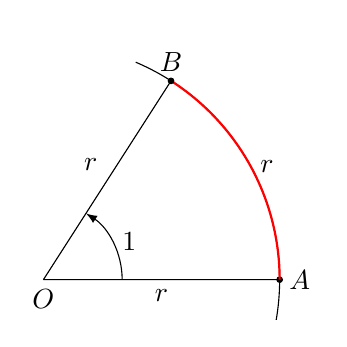
\begin{tikzpicture}
    \clip (-.2,-.5) rectangle (3.5,3.2);
    %% Horizontal
    \draw (0,0) node [below] {$O$} -- node [below] {$r$} (3,0)
    %% point A
    [fill] circle  (1pt) node [below,right] {$A$};

    %% Vue la bizarre façon de faire des arcs, plus simple de rajouter
    %% deux bouts d'arc comme ceci :
    \draw (3,0) arc (0:67:3);
    \draw (3,0) arc (0:-10:3);


    %% Arc  -- Here, 57.3 = 180/pi = 1 rad
    \draw [thick,color=red] (3,0) arc (0:57.3:3); 

    %% point B
    \draw (57.3:3) node [above] {$B$} [fill] circle  (1pt)
    %% Rayon à 1 radian.
    -- node [above left] {$r$} (0,0);

    \draw (1,0) [-latex] arc (0:57.3:1);
    \draw (0,0)
    (28.65:1) node [right] {$\SI{1}{\radian}$} %% 57.3 = 180/pi = 1 rad
    +(28.65:2) node [right] {$r$};
  \end{tikzpicture}\pause\qquad
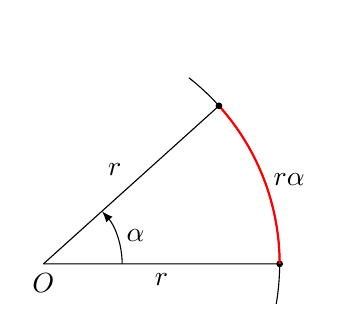
\begin{tikzpicture}
    \def\ALPHA{42}
    \clip (-.2,-.5) rectangle (3.5,3);
    %% Horizontal
    \draw (0,0) node [below] {$O$} -- node [below] {$r$} (3,0)
    %% point A
    [fill] circle (1pt);
    
    %% Vue la bizarre façon de faire des arcs, plus simple de rajouter
    %% deux bouts d'arc comme ceci :
    \draw (3,0) arc (0:\ALPHA+10:3);
    \draw (3,0) arc (0:-10:3);

    %% Arc  -- Here, \ALPHA
    \draw [thick,color=red] (3,0) arc (0:\ALPHA:3); 

    %% point B
    \draw (\ALPHA:3) [fill] circle  (1pt)
    %% Rayon à 1 radian.
    -- node [above left] {$r$} (0,0);

     \draw (1,0) [-latex] arc (0:\ALPHA:1);
     \draw (0,0)
     (.5*\ALPHA:1) node [right] {$\alpha\,\si{\radian}$} %% 57.3 = 180/pi = 1 rad
     +(.5*\ALPHA:2) node [right] {$r \alpha$};
  \end{tikzpicture}
\end{center}\pause

Le radian est idéal pour manipuler des longueurs d'arcs !
\end{frame}

\begin{frame}
  Pour passer du radian au degré et inversement, retenons que $2\pi\,\si{\radian} = \ang{360}$. Par habitude, nous retiendrons également le tableau suivant~:
  \begin{equation*}
    \begin{array}{l|cccccc}\toprule
      \text{en radians} & \sfrac \pi 6 & \sfrac{\pi}{4} & \sfrac{\pi}{3} & \sfrac{\pi}{2}& \pi & 2 \pi\\
      \text{en degrés} & \ang{30} & \ang{45} & \ang{60} & \ang{90} & \ang{180} & \ang{360}\\\bottomrule
    \end{array}
  \end{equation*}
\end{frame}

\section{Fonctions trigonométriques dans le cercle}
\label{sec:cercletrigono}\label{sec:fonctiontrigono}

\begin{frame}
  \begin{definition}
    Un \Defn{cercle trigonométrique} est un cercle de rayon $1$, il permet de représenter géométriquement toutes les fonctions trigonométriques.

    Ces fonctions sont les fonctions sinus, cosinus, tangente, cotangente, sécante, cosécante et quelques autres plus rarement utilisées.
  \end{definition}

\begin{center}
  \includegraphics[trim=0 50 0 0,clip]{fonctionstrigo}
\end{center}
\end{frame}

\begin{frame}
  Autres fonctions trigonométriques :
  \begin{align*}
    \tan(\theta) &= \frac{\sin(\theta)}{\cos(\theta)} & \sec(\theta) &= \frac{1}{\cos(\theta)}\\
    \cot(\theta) &= \frac{\cos(\theta)}{\sin(\theta)} & cosec(\theta) &= \frac{1}{\sin(\theta)}
  \end{align*}

  Attention au domaine !
\end{frame}

\begin{frame}
\begin{center}
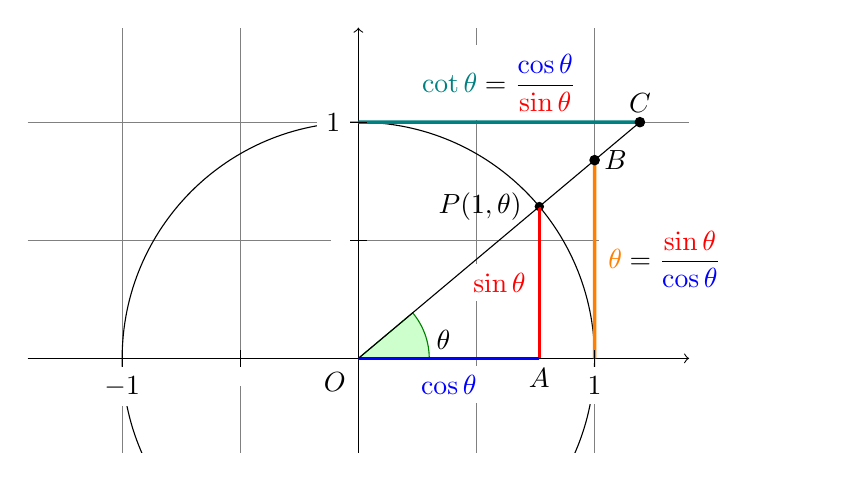
\begin{tikzpicture}[scale=3] 
\def\th{40} %% CHANGER LE CAPTION ACCORDINGLY !!
\def\diamdepoint{0.02}

\clip (-1.4,-0.4) rectangle (2,1.4);
\draw[step=0.5,gray,very thin] (-1.4,-1.4) grid (1.4,1.4);

%% petit arc vert
\filldraw[fill=green!20,draw=green!50!black] (0,0) -- (0.3,0) arc 
(0:\th:0.3) -- cycle; 
\node [right] at (15:0.3) {$\theta$};

%% Point P
\node[left=.1cm] at (\th:1) {$P (1,\theta)$};
\fill (\th:1) circle (\diamdepoint);

%% axes
\draw[->] (-1.4,0) -- (1.4,0) coordinate (x axis); 
\draw[->] (0,-1.4) -- (0,1.4) coordinate (y axis); 

%% grand cercles
\draw (0,0) circle (1); 

%% 
\draw[very thick,red] 
(\th:1) -- node[left=1pt,fill=white] {$\sin \theta$} (\th:1 |- x axis)
coordinate (A); 
%% 
\draw[very thick,blue] 
(\th:1 |- x axis) -- node[below=2pt,fill=white] {$\cos \theta$} (0,0); 
%%
\draw[very thick,orange] (1,0) -- node [right=1pt,fill=white] 
{$\displaystyle \tg \theta \color{black}= 
\frac{{\color{red}\sin \theta}}{\color{blue}\cos \theta}$} 
(intersection of 0,0--\th:1 and 1,0--1,1) coordinate (t); 


%%
\draw[very thick,color=green!50!blue] (0,1) -- node [fill=white,above] 
{$\displaystyle \cot \theta \color{black}= 
\frac{{\color{blue}\cos \theta}}{\color{red}\sin \theta}$} 
(intersection of 0,0--\th:1 and 0,1--2,1) coordinate (c); 

\draw (0,0) -- (c) -- (t); %% Aller le plus loin : tan ou cot.
\node[right] at (t) {$B$};
\draw[fill] (t) circle (\diamdepoint);
\node[above] at (c) {$C$};
\draw[fill] (c) circle (\diamdepoint);
\foreach \x/\xtext in {-1, -0.5/{}, 1} 
\draw (\x,1pt) -- (\x,-1pt) node[anchor=north,fill=white] {$\xtext$}; 
\foreach \y/\ytext in {-1, -0.5/, 0.5/, 1} 
\draw (1pt,\y) -- (-1pt,\y) node[anchor=east,fill=white] {$\ytext$}; 
\node at (-0.1, -0.1) {$O$};
\node[below] at (A) {$A$};
\end{tikzpicture} 
\end{center}
\end{frame}

\begin{frame}{Angles remarquables}
  Les fonctions trigonométriques les plus utilisées :
  \begin{align*}
  \sin &\colon \RR \vers [-1,1]\hspace*{2cm}&  \tan &\colon
  \RR\setminus\set{\frac\pi2 + k\pi \telque k \in \ZZ} \vers \RR \\ 
  \cos &\colon \RR \vers [-1,1]& \cot &\colon
  \RR\setminus\set{k\pi \telque k \in \ZZ} \vers \RR.
\end{align*}
(L'ensemble d'arrivée a été choisi = ensemble image.)\pause

Voici quelques valeurs importantes des fonctions sinus et cosinus :
\begin{equation}\label{valeurscossin}
  \begin{array}{c|rl|c|c|c}
    \hline 
    \text{angle} & \sin & & \cos & \tan & \cot\\
    \hline
    0          &\sfrac {\sqrt 0}{2}& = 0& 1 & 0 & \nexists\\
    \sfrac \pi 6&\sfrac {\sqrt 1}{2}& = \sfrac12 &\sfrac {\sqrt 3}{2} &\sfrac {\sqrt 3}{3}& \sqrt 3\\
    \sfrac \pi 4&\sfrac {\sqrt 2}{2}& & \sfrac {\sqrt 2}{2} & 1 &1\\  
    \sfrac \pi 3&\sfrac {\sqrt 3}{2}& & \sfrac 1 2 &\sqrt 3 & \sfrac {\sqrt 3}{3}\\ 
    \sfrac \pi 2&\sfrac {\sqrt 4}{2}& = 1&0&\nexists&0\\
    \hline
  \end{array} 
\end{equation}
\end{frame}

\begin{frame}{Pente et angle}
  \begin{proposition}
    Étant donné un repère cartésien orthonormé. Pour une droite d'équation \(y = ax + b\) formant un angle \(\theta\) avec l'horizontale, nous avons
    \begin{equation*}
      a = \tan \theta
    \end{equation*}
  \end{proposition}

  \begin{tabular}{lc}
  \begin{minipage}{0.3\linewidth}
    \[a = \frac{\Delta y}{\Delta x} = \frac{y_1-y_0}{x_1-x_0}\] où $(x_0, y_0)$ et $(x_1,y_1)$ sont deux points distincts du graphe de $f$.
  \end{minipage}
  \begin{minipage}{0.65\linewidth{}}
    \def\xmax{5}%
    \def\ymax{2}%
  \begin{tikzpicture}
    \draw (0,0) node [below left] {$0$};%
    \foreach \y in {1, ..., \ymax} \draw (3pt,\y) -- (-3pt,\y) node
    [left] {$\y$};%
    \foreach \x in {1, ..., \xmax} \draw (\x,3pt) -- (\x,-3pt) node
    [below] {$\x$};%
    \draw [->] (0,-.2) -- (0,\ymax+1) node [above left] {$y$};%
    \draw [->] (-.2,0) -- (\xmax+1,0) node [below right] {$x$};%
    \begin{scope}[shift={+(1,0)}]
      \draw (35:-1) -- (35:4);%
      \draw[->] (.5,0) arc (0:35:.5) node [right] {$\theta$};%
      \coordinate (A) at (35:3);%
    \end{scope}
    \draw
    [dotted]
    [postaction={%
      decorate,draw,solid,
      decoration={brace, raise=2pt}      
    }]
    (A) -- (A|-0,0) node [midway,right=3pt] {$\Delta y$};%
    \draw
    [dotted]
    [postaction={%
      decorate,draw,solid,
      decoration={brace, raise=15pt, mirror}
    }]
    (1,0) -- (A|-0,0) node [midway,below=15pt] {$\Delta x$};%
  \end{tikzpicture}
\end{minipage}
\end{tabular}
\end{frame}

\begin{frame}
  \begin{remark*}
 Cette interprétation ne tient plus si les axes ne sont
pas gradués à l'identique :
\end{remark*}
%% CVV : développer car ils font régulièrement l'erreur
%% NR : je veux bien, mais que dire d'autre si ce n'est que c'est faux en donnant un exercice à faire ? Cela dit je reformulerai la section afin d'avoir plus de clarté.
\begin{center}
    \def\xmax{4}%
    \def\ymax{3}%
  \begin{tikzpicture}[xscale=2]
    \draw (0,0) node [below left] {$0$};%
    \foreach \y in {1, ..., \ymax} \draw (3pt,\y) -- (-3pt,\y) node
    [left] {$\y$};%
    \foreach \x in {1, ..., \xmax} \draw (\x,3pt) -- (\x,-3pt) node
    [below] {$\x$};%
    \draw [->] (0,-.2) -- (0,\ymax+1) node [above left] {$y$};%
    \draw [->] (-.2,0) -- (\xmax+1,0) node [below right] {$x$};%
    \begin{scope}[shift={+(1,0)}]
      \draw (35:-1) -- (35:4);%
      \draw[->,xscale=.5] (1,0) arc (0:19.3:1) node [right] {${\pmb ?}$};%
    \end{scope}
  \end{tikzpicture}
\end{center}
\end{frame}

\section{Diagrammes de Venn — Patatoïdes convexes}
\begin{frame}{Diagrammes de Venn}% FIXME: présenté comme ceci ça sert à rien. Voir plus loin pour un truc meilleur.
\begin{exercise}
  Voici deux diagrammes de Venn :
  \begin{center}
    \raisebox{-.5\height}{\begin{venndiagram2sets}[shade=red]
      \fillACapB
    \end{venndiagram2sets}}
    \raisebox{-.5\height}{\begin{venndiagram3sets}[shade=green]
      \fillOnlyA
    \end{venndiagram3sets}}
  \end{center}
  Que représentent-ils ?
\end{exercise}
\end{frame}

\section{Interprétation de la notion de fonction}
\begin{frame}
  Distinguons deux manières de \og voir\fg{} les fonctions~:
  \begin{description}
  \item[Association] La fonction réalise l'association : à l'objet $x \in A$, la fonction $f$ associe une valeur ou un objet noté $f(x)$.\pause
  \item[Transformation] Le domaine est \og déplacé\fg{} dans l'ensemble d'arrivée.
  \end{description}
\end{frame}

\begin{frame}
  \begin{block}{Association}
  À chaque point du plan, on associe deux réels : ses coordonnées cartésiennes!

  \begin{equation*}
    f : \text{plan} \to \RR^2 : P \mapsto (P_{1},P_{2})
  \end{equation*}
\end{block}
\begin{block}{Transformation}
 Chaque point du plan (de coordonnées données) est envoyé sur un autre point du plan (dont on donne les coordonnées).

  \begin{equation*}
    f : \RR^{2} \to \RR^2 : (x,y) \mapsto (-y,x)
  \end{equation*}
  \pause

  On a mélangé \og point\fg{} et \og coordonnées du point\fg{} !\pause

  \begin{equation*}
    g : \RR^{2} \to \RR^2 : (x,y) \mapsto (x,0)
  \end{equation*}
  \pause \(g\) n'est pas injective.
\end{block}
\end{frame}

\section{Géométrie analytique}
\begin{frame}
  \begin{definition}
    La géométrie analytique est une manière d'aborder des problèmes de géométrie grâce à un ou plusieurs systèmes de coordonnées.
  \end{definition}

  Nous commencerons par le système de coordonnées cartésiennes.
\end{frame}

\section{Points}
\label{sec:vect-vers-points}
\begin{frame}
\begin{definition}
Un élément de \(\RR^{n}\) peut être vu comme un \Defn{point}, il s'écrit avec \(n\) nombres réels appelés ses \Defn{coordonnées}, que nous notons généralement \((p_{1}, p_{2}, \ldots, p_{n})\).

Lorsque \(n = 2\), les coordonnées sont : abcisses et ordonnées.
\end{definition}

\begin{example}
   Le point \((1,-1)\) de \(\RR^{2}\) désigne l'élément du plan d'abcisse \(1\) et d'ordonnée \(-1\).
\end{example}
\end{frame}

\section{Vecteurs}
\begin{frame}
  \begin{definition}
    Un élément de \(\RR^{n}\) peut être vu comme un \Defn{vecteur}, et ses constituants sont les \Defn{composantes} du vecteur.
\end{definition}

\begin{remark}
  Un vecteur représente un déplacement : une translation.
\end{remark}

\begin{example}
 Le vecteur \((-1,1)\) de \(\RR^{2}\) indique une translation dans la direction \og Nord-Ouest\fg{} sur le plan.
\end{example}
\end{frame}


\begin{frame}
  \begin{block}{Différence entre point et vecteur}
La différence, fondamentale et intuitive, entre point et vecteur est que le premier représente un état, une position ; tandis que le second représente une évolution, un mouvement.
\end{block}

\begin{remark}
  Les deux sont représentés par des éléments de \(\RR^n\) !
\end{remark}
\end{frame}

\subsection{Vecteurs libres vs vecteurs liés}
\begin{frame}
  Un vecteur se représente généralement par une flèche.\pause

  Un vecteur peut être
  \begin{itemize}
  \item basée en un point (on la dessine en un endroit donné), ou\pause
  \item être libre (représente une direction générale, sans point de départ particulier)
\end{itemize}
\end{frame}

\section{Opérations de base}
\begin{frame}
  Si \(\vec {x}\) et \(\vec {y}\) sont des éléments de \(\RR^{n}\) et \(\lambda\in \RR\), on définit
  \begin{align*}
    (x_{1}, \ldots, x_{n}) + (y_{1}, \ldots, y_{n}) &= (x_{1}+y_{1}, \ldots, x_{n}+y_{n}) \\
    (x_{1}, \ldots, x_{n}) - (y_{1}, \ldots, y_{n}) &= (x_{1}-y_{1}, \ldots, x_{n}-y_{n}) \\
    \lambda\, (x_{1}, \ldots, x_{n}) &= (\lambda x_{1}, \ldots, \lambda x_{n})
  \end{align*}
\end{frame}

\begin{frame}
  \begin{itemize}
  \item la somme de deux vecteurs est donnée par la règle du parallélogramme ;
  \item la multiplication par un réel (on dira aussi \og par un \Defn{scalaire}\fg{}) multiplie la longueur.
  \end{itemize}

  \begin{center}
    \includegraphics{somme-vecteurs}
  \end{center}
\end{frame}

\begin{frame}
\begin{itemize}
%\item la somme de deux \emph{points} n'a pas de sens intuitif ;
\item la différence de deux \emph{points} est un vecteur allant du second vers le premier : \(\point p - \point q\) est le vecteur \(\fleche{qp}\) ;
\item la somme d'un \emph{point} et d'un \emph{vecteur} représente un déplacement à partir de ce point dans la direction du vecteur donné : le résultat est un point ;
\item la somme de deux ou plusieurs \emph{vecteurs} représente la composée de déplacements successifs : le résultat est un vecteur.
\end{itemize}

\begin{example}
  Si on considère $\point p = (1,2)$ comme un point, et \(\vec w = (1,-1)\) comme un vecteur (donnant la direction \og Nord-Ouest\fg{}), alors on conçoit leur somme \(\point p + \vec w = (1,2) + (1,-1) = (2,1)\) comme le point obtenu en translatant le point de départ, \(\point p\), dans la direction donnée \(\vec w\).
\end{example}
\end{frame}

\begin{frame}
  \begin{definition}
    L'élément particulier \((0, 0, \ldots, 0)\) se note \(\vec 0\) et est appelé \Defn{vecteur nul}.
  \end{definition}

  \begin{proposition}Quel que soit le vecteur \(\vec x\in \RR^{n}\), nous avons
    \begin{equation*}
      x + \vec 0 = \vec 0 + x = x.
    \end{equation*}
  \end{proposition}
\end{frame}

\begin{frame}
  Regardons le cas \(n = 3\).\pause

  Si nous notons \(\vec {e_{1}}, \vec {e_{2}}, \vec {e_{3}}\) les vecteurs suivants~:
  \begin{align*}
    \vec {e_{1}} &= (1, 0, 0) & \vec {e_{2}} &= (0, 1, 0) & \vec {e_{3}} &= (0, 0, 1)
  \end{align*}\pause
  alors tout vecteur \(\vec x\) de \(\RR^{3}\) peut s'écrire \(x_{1}\vec {e_{1}} + x_{2} \vec {e_{2}} + x_{3} \vec {e_{3}}\).

\pause  On peut généraliser à d'autres valeurs de \(n\)
\pause
\begin{remark*}
  Attention, ici \(\vec {e_{1}}\) et ses compagnons ne sont pas les composante d'un hypothétique vecteur \(e\), mais des vecteurs eux-même ! Pour l'exemple, \(x_{1}\) et \(\vec {e_{1}}\) ont donc des rôles fondamentalement différents : le premier est un réel (ou \og scalaire\fg{}), le second est un vecteur.
\end{remark*}
\end{frame}

% \begin{proposition}
%   Tout vecteur \(\vec v\) de \(\RR^{n}\) s'écrit
%   \begin{equation*}
%     v_{1} \vec {e_{1}} + \cdots + v_{n} \vec {e_{n}}
%   \end{equation*}
%   où \(\vec {e_{i}}\) est un vecteur de \(\RR^{n}\) dont la \(j\)\ieme{} composante vaut \(0\) si \(i \neq j\), et vaut \(1\) si \(i = j\) ; en d'autres termes
%   \begin{equation*}
%     \paren{e_{i}}_{j} =
%     \begin{cases}
%       1 & \text{si \(i = j\)} \\
%       0 & \text{sinon.}
%     \end{cases}
%   \end{equation*}
% \end{proposition}

% \begin{frame}
% \begin{definition}
%   Si \(\vec{u_{1}}, \ldots, \vec{u_{k}}\) sont des vecteurs, une \Defn{combinaison linéaire} de ceux-ci est une somme de la forme \(\lambda_{1} \vec{u_{1}} + \cdots + \lambda_{k} \vec{u_{k}}\).
% \end{definition}

% \begin{remark*}
%   On peut paraphraser la proposition précédente sous la forme : tout vecteur \(\vec v \in \RR^{n}\) est une combinaison linéaire des vecteurs \(\vec{e_{1}},\ldots,\vec{e_{n}}\).
% \end{remark*}
% \end{frame}

\section{Produit scalaire}\label{sec:produit-scalaire}
\subsection{Définition}
\begin{frame}
\begin{definition}
  Le \Defn{produit scalaire} entre deux vecteurs \(\vec v\) et \(\vec w\) de \(\RR^{n}\) est donné par
  \begin{equation*}
    \scalprod {\vec v} {\vec w} = v_{1} w_{1} + \cdots + v_{n} w_{n}.
  \end{equation*}
\end{definition}

\begin{proposition}Pour tous vecteurs \(\vec a,\vec {a'},\vec b \in \RR^{n}\) et \(\lambda, \mu \in \RR\), le produit scalaire vérifie les propriétés suivantes :
  \begin{enumerate}
  \item $\scalprod{(\lambda \vec{a} + \mu \vec{a'})}{\vec{b}} = \lambda \scalprod{\vec{a}}{\vec{b}} + \mu \scalprod{\vec{a'}}{\vec{b}}$ (linéaire à gauche)
  \item $\scalprod{\vec{a}}{\vec{b}}=\scalprod{\vec{b}}{\vec{a}}$ (symétrique)
  \item $\scalprod{\vec{a}}{\vec{a}} \geq 0$ et de plus, $\scalprod{\vec{a}}{\vec{a}} = 0 \iff \vec{a} = \vec 0$ (défini positif).
  \end{enumerate}
\end{proposition}
Notons que les deux premières propriétés montrent qu'il y a également linéarité à droite ; on dit alors que le produit scalaire est \Defn{bilinéaire}.
\end{frame}
\course{4}
\begin{frame}%% pour le cours de lundi
  \begin{block}{Information importantes pour les BA1 Informatique}
    Le cours de programmation de Thierry Massart de ce lundi commencera à 10h30.
  \end{block}
\end{frame}
\begin{frame}
  \begin{definition}(Rappel). 
    Étant donné un angle \(\theta\) en radians, on définit son cosinus et son sinus comme les coordonnées du point \(P_{\theta}\) tel que l'angle \(\widehat{IOP}\) est de mesure \(\theta\), où \(I = (1,0)\) et \(O = (0,0)\).
  \end{definition}\pause

  \begin{proposition}Pour des angles \(\theta\) et \(\varphi\), on a :
    \begin{equation*}
      \cos (\theta + \varphi) = \cos \theta \cos \varphi - \sin \theta \sin \varphi
    \end{equation*}
  \end{proposition}\pause

  Avant de prouver ce résultat, nous allons expliciter les quelques relations \og évidentes\fg{} des sinus et cosinus.
\end{frame}
\section{Relation fondamentale}
\begin{frame}
  Le théorème de Pythagore appliqué dans le cercle trigonométrique implique l'importante relation $(\cos(\theta))^2 + (\sin(\theta))^2 = 1$, ce qu'on écrira plus souvent sous la forme
  \begin{equation*}
    \cos^2\theta + \sin^2 \theta  = 1.
  \end{equation*}
\end{frame}

\section{Symétries}
\subsection{Symétrie par rapport à l'axe des abscisses}
\begin{frame}
\begin{minipage}{0.5\linewidth}
\centering
\scalebox{0.75}{\input{cercle-1.pdf_t}}
\end{minipage}
\begin{minipage}{0.45\linewidth}
\centering

\begin{align*}
\sin\paren*{ -x}&=-\sin\paren*{ x} \\
\cos\paren*{ -x}&=\cos\paren*{ x} \\ 
\tan\paren*{ -x}&=-\tan\paren*{ x}
\end{align*}
\end{minipage}
\end{frame}
\subsection{Symétrie par rapport à l'axe des ordonnées}
\begin{frame}
\begin{minipage}{0.5\linewidth}
\centering
\scalebox{0.75}{\input{cercle-2.pdf_t}}
\end{minipage}
\begin{minipage}{0.45\linewidth}
\centering
\[\begin{array}{c}
\sin\paren*{ \pi -x} =\sin\paren*{ x} \\
\\
\cos\paren*{ \pi -x} =-\cos\paren*{ x} \\
\\
\tan\paren*{ \pi -x} =-\tan\paren*{ x}
\end{array}\]
\end{minipage}
\end{frame}
\subsection{Symétrie par rapport à l'origine}
\begin{frame}
\begin{minipage}{0.5\linewidth}
\centering
\scalebox{0.75}{\input{cercle-3.pdf_t}}
\end{minipage}
\begin{minipage}{0.45\linewidth}
\centering
\[\begin{array}{c}
\sin\paren*{ \pi +x} =-\sin\paren*{ x} \\ \\
\cos\paren*{ \pi +x} =-\cos\paren*{ x} \\ \\
\tan\paren*{ \pi +x} =\tan\paren*{ x}
\end{array}\]
\end{minipage}
\end{frame}
\subsection{Symétrie par rapport à la première bissectrice}
\begin{frame}
\begin{minipage}{0.58\linewidth}
\centering
\scalebox{0.75}{\input{cercle-4.pdf_t}}
\end{minipage}
\begin{minipage}{0.40\linewidth}
\centering
\[\begin{array}{c}
\sin\paren*{ \dfrac{\pi}{2} -x} =\cos\paren*{ x} \\ \\
\cos\paren*{ \dfrac{\pi}{2} -x} =\sin\paren*{ x} \\ \\
\tan\paren*{ \dfrac{\pi}{2} -x} =\cot\paren*{ x}
\end{array}\]
\end{minipage}
\end{frame}

\subsection{Angles décalés de 90\degre}
\begin{frame}
\begin{minipage}{0.5\linewidth}
\centering
\scalebox{0.75}{\input{cercle-5.pdf_t}}
\end{minipage}
\begin{minipage}{0.45\linewidth}
\centering
\[\begin{array}{c}
\sin\paren*{ \dfrac{\pi}{2} +x} =\cos\paren*{ x} \\
\\
\cos\paren*{ \dfrac{\pi}{2} +x} =-\sin\paren*{ x} \\
\\
\tan\paren*{ \dfrac{\pi}{2} +x} =-\cot\paren*{ x}
\end{array}\]
\end{minipage}
\end{frame}

\begin{frame}% FIXME: intégrer au syllabus
  \begin{proof}[Preuve de la formule d'addition]
    Nous voulons prouver
    \begin{math}
      \cos (\theta + \varphi) = \cos \theta \cos \varphi - \sin \theta \sin \varphi.
    \end{math}\par\pause
    \begin{minipage}{0.66\linewidth}
      Dans un repère cartésien, notons
      \begin{itemize}
      \item \(\vec{o} = (0,0)\), \(\vec{a} = (1,0)\), \(\vec{b} = (0,1)\),
      \item \(
        \begin{aligned}[t]
          \vec{p} &= % (\cos(\theta),\sin(\theta))= 
          \cos(\theta) \vec{a} + \sin(\theta) \vec{b}
        \end{aligned}\)
      \item \(\vec{q} = (\cos(\theta + \varphi),\sin(\theta + \varphi))\)
      \item \(
        \begin{aligned}[t]
          \vec{r} &= (\cos(\theta + \pi/2),\sin(\theta + \pi/2))\\
          &= (-\sin(\theta),\cos(\theta))
        \end{aligned}\)
      \end{itemize}
    \end{minipage}
    \begin{minipage}{0.33\linewidth}
      \includegraphics[width=\linewidth]{cosdesomme}
    \end{minipage}\pause

    Dans le repère tourné d'un angle \(\theta\), on observe
    \begin{math}
      \vec{q} = \cos(\varphi) \vec{p} + \sin(\varphi)\vec{r},
    \end{math}
    et donc
    \vspace*{-2.5ex}
    \begin{align*}
      (\cos(\theta& + \varphi),\sin(\theta + \varphi))\\
      &= \cos(\varphi) \, (\cos(\theta),\sin(\theta)) + \sin(\varphi) \, (-\sin(\theta),\cos(\theta))\\
      &= (\cos(\varphi) \cos(\theta) - \sin(\varphi) \sin(\theta), \cos(\varphi) \sin(\theta) + \sin(\varphi)\cos(\theta))
    \end{align*}
    ce qui démontre la relation proposée, ainsi que la relation similaire concernant \(\sin(\varphi+\theta)\).
  \end{proof}
\end{frame}
\begin{frame}
  \vspace{-3.ex}
  \begin{align*}
    \sin (A + B)      & = \sin A \cos B + \cos A \sin B                                                      \\
    \cos (A + B)      & = \cos A \cos B - \sin A \sin B                                                      \\
    \tan (A + B)      & = \frac{\tan A + \tan B}{1 - \tan A \tan B}                                          \\
    % \sin (3a) & = 3\sin a -4 \sin^{3} a \\
    % \cos (3a) & = -3\cos a +4 \cos^{3} a \\
    \cos A \cos B     & =\frac{\cos(A-B)+\cos(A+B)}2\\
    \sin A \sin B     & =\frac{\cos(A-B)-\cos(A+B)}2\\
    \sin A \cos B     & =\frac{\sin(A+B)+\sin(A-B)}2                                                        \\
    \cos A \sin B     & =\frac{\sin(A+B)-\sin(A-B)}2                                                         \\
    \cos p + \cos q   & = 2 \cos \paren*{ \frac{p+q} 2 } \cos \paren*{ \frac{p-q} 2 }                        \\
    \cos p - \cos q   & = -2 \sin \paren*{ \frac{p+q} 2 } \sin \paren*{ \frac{p-q} 2 }                       \\
    \sin p + \sin q   & = 2 \sin \paren*{ \frac{p+q} 2 } \cos \paren*{ \frac{p-q} 2 }
    % \sin p - \sin q & = 2 \cos \paren*{ \frac{p+q} 2 } \sin \paren*{ \frac{p-q} 2 } \\
  \end{align*}
\end{frame}
\begin{frame}
  \begin{definition}
    Le \Defn{produit scalaire} entre deux vecteurs \(\vec v\) et \(\vec w\) de \(\RR^{n}\) est donné par
    \begin{equation*}
      \scalprod {\vec v} {\vec w} = v_{1} w_{1} + \cdots + v_{n} w_{n}.
    \end{equation*}
  \end{definition}

  \begin{example}
    \begin{equation*}
      \scalprod{(2,1)}{(2,5)} = 2 \cdot 2 + 1 \cdot 5 = 9
    \end{equation*}\pause
  \begin{equation*}
    \scalprod{(1,0)}{(2,5)} = 2
  \end{equation*}\pause
  \begin{equation*}
    \scalprod{(0,1)}{(2,5)} = 5
  \end{equation*}\pause
  Si \(\vec{v} = (v_{1},v_{2}, \ldots, v_{n})\), on a \(\scalprod{\vec{v}}{\vec{e_{i}}} = v_{i}\)

  Rappel : 
  \(\paren{e_{i}}_{j} =
    \begin{cases}
      1 & \text{si \(i = j\)} \\
      0 & \text{sinon.}
    \end{cases}
    \qquad \vec{e_{i}} = (0,\ldots,0,{\underbrace{1}_{\mathclap[\displaystyle]{\text{\(i\)-ème pos}}}},0,\ldots,0)\)
\end{example}
\end{frame}

\begin{frame}
  On définit la \Defn{norme} (associée à ce produit scalaire) par :
  \begin{equation*}
    \norme {\vec v} \pardef \sqrt{\scalprod{\vec v}{\vec v}} = \sqrt{v_{1}^{2}  + \cdots + v_{n}^{2}}
  \end{equation*}\pause
  Cette norme vérifie donc la propriété \(\norme{\vec v} = 0 \iff \vec v = 0\).\pause

  \begin{remark*}
    La \og norme\fg{} d'un vecteur correspond à sa \og longueur\fg{} d'après le théorème de Pythagore.
  \end{remark*}\pause

  \begin{example}
    Pour \(n = 2\), si \((a,b) \in \RR^2\), on a \(\norme{(a,b)} = \sqrt{a^{2} + b^{2}}\).
  \end{example}
\end{frame}

\begin{frame}
  \begin{proposition}[Inégalité de Cauchy-Schwarz]Pour tout \(\vec a, \vec b\) de \(\RR^{n}\), on a 
    \begin{equation*}
      \abs{\scalprod{\vec a}{\vec b}} \leq \norme {\vec a} \norme {\vec b}.
    \end{equation*}
  \end{proposition}
\end{frame}
\begin{frame}
  \begin{proof}
    Considérons la quantité \(\scalprod{\vec a + t \vec b}{\vec a + t \vec b}\), qui est positive.
    \pause Nous pouvons la ré-écrire via la bilinéarité du produit scalaire sous la forme~:
    \begin{align*}
      \scalprod{\paren*{\vec a + t \vec b}}{\paren*{\vec a + t \vec b}} &= \scalprod {\vec a}{\vec a} + 2 t \scalprod{\vec a}{\vec b} + t^{2} \scalprod{\vec b}{\vec b}\\
                                                                        & = \norme{\vec{a}}^{2} + 2 t \scalprod {\vec a}{\vec b} + t^{2} \norme{\vec{b}}^{2} \\
                                                                        & = \paren*{t \norme{\vec{b}} + \frac{\scalprod{\vec a}{\vec b}}{\norme{\vec{b}}}}^{2} - \paren*{\frac{\scalprod{\vec a}{\vec b}}{\norme{\vec{b}}}}^{2} + \norme{\vec{a}}^{2} \geq 0
    \end{align*}\pause
    En choisissant \(t = - \frac{\scalprod {\vec a}{\vec b}}{\norme{\vec{b}}^{2}}\), on obtient
    \begin{math}
      \norme{\vec{a}}^{2} \geq \paren*{\frac{{\scalprod{\vec a}{\vec b}}}{\norme{\vec{b}}}}^{2},
    \end{math}\pause
    d'où
    \begin{equation*}
      \norme{\vec{a}} \geq \frac{\abs{\scalprod{\vec a}{\vec b}}}{\norme{\vec{b}}}
    \end{equation*}
    qui est l'inégalité annoncée.
  \end{proof}
\end{frame}
\begin{frame}
  \begin{proposition}
    La norme \(\norme \cdot : \RR^{n} \to \RR\) vérifie les propriétés suivantes~:
    \begin{itemize}
    \item \(\norme{\vec a} = 0 \iff \vec a = \vec 0\) ;
    \item \(\norme{\lambda \vec a} = \abs \lambda \norme{\vec a}\) ;\pause
    \item \(\norme{\vec a + \vec b} \leq \norme{\vec a} + \norme{\vec b}\) (inégalité triangulaire).
    \end{itemize}
  \end{proposition}\pause
  \begin{proof}
    Les deux premières propriétés sont évidentes de la définition de la norme et les propriétés du produit scalaire. \pause La troisième se démontre en calculant
    \begin{align*}
      \norme{\vec a + \vec b}^{2} &= \scalprod{\vec a + \vec b}{\vec a + \vec b}\\
                                  & = \scalprod{\vec a}{\vec a} + \scalprod{\vec b}{\vec b} + 2 \scalprod{\vec a}{\vec b} \\
                                  & \leq \scalprod{\vec a}{\vec a} + \scalprod{\vec b}{\vec b} + 2 \norme{\vec a}\norme{\vec b}\\
                                  &= \paren*{\norme {\vec a} + \norme {\vec b}}^{2}
    \end{align*}
    où nous avons utilisé l'inégalité de Cauchy-Schwarz.
  \end{proof}
\end{frame}
\begin{frame}
  \begin{remark*}
    Lorsque ce n'est pas indiqué, les vecteurs sont imaginés basés au même point (généralement en l'origine).
  \end{remark*}
\end{frame}
\begin{frame}
\begin{proposition}
  Si \(\vec v\) et \(\vec w\) sont des vecteurs de \(\RR^{n}\), alors
  \begin{equation*}
    \scalprod{\vec v}{\vec w} = \norme {\vec v}\norme{\vec w} \cos(\theta)
  \end{equation*}
  où \(\theta\) est l'angle formé par les vecteurs \(\vec v\) et \(\vec w\).
\end{proposition}\pause
\begin{remark}
  Si \(\vec{v}\) est un vecteur quelconque du plan (basé en l'origine), alors \(\frac{\vec{v}}{\norme{v}}\) est de norme \(1\), et donc de la forme \((\cos\phi,\sin\phi)\) pour un certain angle \(\phi\).
\end{remark}\pause
\begin{proof}[Preuve de la proposition en dimension \(2\)]
  Si \(\vec v = (\norme {\vec v} \cos(\phi), \norme {\vec v} \sin(\phi))\) et  \(\vec w = (\norme {\vec w} \cos(\psi), \norme {\vec w} \sin(\psi))\), alors 
  \begin{equation*}
    \scalprod{\vec v}{\vec w} = \norme{\vec v}  \norme{\vec w} (\cos(\phi)\cos(\psi) + \sin(\phi)\sin(\psi)) = \norme{\vec v}\norme{\vec w} \cos{\paren{\psi-\phi}}
  \end{equation*}
  où \(\psi-\phi\) représente bien l'angle entre les deux vecteurs.
\end{proof}
\end{frame}

\begin{frame}
  \begin{corollary}
    Le produit scalaire s'annule si et seulement si les vecteurs sont orthogonaux (ou si l'un des deux vecteurs est nul).
  \end{corollary}
  \begin{proof}
    Rappelons le résultat :
    \begin{equation*}
      \scalprod{\vec v}{\vec w} = \norme {\vec v}\norme{\vec w} \cos(\theta)
    \end{equation*}

    Si les vecteurs ne sont pas nuls, alors leur norme n'est pas nulle, dès lors seul le cosinus peut s'annuler, ce qui n'arrive que pour des angles droits.
  \end{proof}
\end{frame}

\begin{frame}% FIXME: intégrer au syllabus dans la partie A ? (ça se trouve dans le module T)
  \begin{corollary}La projection orthogonale d'un vecteur \(\vec{v}\) sur (la droite engendrée par) un vecteur \(\vec{w}\) est
    \(\vec p = \frac{\scalprod{\vec{v}}{\vec{w}}}{\norme{w}^{2}} \vec{w}\).
  \end{corollary}\pause
  \begin{proof}
    Le projeté sera du type \(\vec{p} = k \vec{w}\) pour un certain \(k\).\pause
    
    On veut que \(\vec{v} - \vec{p}\) soit orthogonal à \(\vec{w}\).\pause

    On écrit l'égalité correspondante, et la valeur de \(k\) en découle.

    \begin{equation*}
      \scalprod{\vec{v}-\vec{p}}{\vec{w}} = 0 \iff \scalprod{\vec{v}}{\vec{w}} = \scalprod{k\vec{w}}{\vec{w}} = k \norme{\vec{w}}^{2}
    \end{equation*}
  \end{proof}
\end{frame}

\begin{frame}{Centre de gravité}% FIXME: intégrer au syllabus
  \begin{definition}
    Si on considère des points \(\point{P}_{1}, \ldots, \point{P}_{k}\) dans \(\RR^n\), leur centre de gravité est :
    \begin{equation*}
      \point{O} + \frac{1}{k}\sum_i \vec{OP_{i}}
    \end{equation*}
    où \(O\) représente n'importe quel point de l'espace (souvent on prend l'origine).
  \end{definition}\pause
  \begin{remark*}
    Pouvez-vous démontrer que la quantité ci-dessus ne dépend pas du point \(O\) choisi ?
  \end{remark*}\pause
  \begin{example}
    Le centre de gravité de \((1,1), (1,-1),(-1,1), (-1,-1)\) est l'origine.
  \end{example}
\end{frame}
\section{Équations et systèmes}
\begin{frame}
\begin{definition}
  Une \Defn{équation} est une égalité faisant intervenir une ou plusieurs quantités inconnues.\pause

  Résoudre une équation revient à déterminer l'ensemble des valeurs possibles pour la quantité inconnue de sorte que l'égalité soit vérifiée. Ces valeurs sont les \Defn{solutions} de l'équation.
\end{definition}

Dans une de ses formes les plus simples, une équation fait intervenir une unique quantité inconnue : un nombre réel. La \og quantité inconnue\fg{} (ou simplement \og inconnue\fg{}) est souvent nommée \(x\), mais ce nom n'a rien de magique.
\end{frame}
\begin{frame}
\begin{example}
  \begin{itemize}[<+->]
  \item L'équation \(2x - 3 = 1\) a pour seule solution : \(x = 2\).
  \item L'équation \(t^{2} - 1 = 0\) (dont l'inconnue est \(t\)) a pour solutions : \(t = 1\) et \(t = -1\). On peut écrire que l'ensemble des solutions est \(S = \set{-1,1}\).
  \item L'équation \(\sin(x) = 0\) a pour solution \(x = 0\), mais il y en a d'autres. \pause Par exemple \(x = \pi\). \pause En fait, l'ensemble des solutions est formé de l'ensemble des multiples entiers de \(\pi\). On peut noter \(S = \set{k \pi \telque k \in \ZZ}\).
  \item L'équation \(x^{2} + 1 = 0\) n'a pas de solution dans les nombres réels, car tout réel pris au carré est positif, donc \(x^{2}+1\) ne peut jamais être égal à \(0\). L'ensemble des solutions est donc vide. On peut noter \(S = \emptyset\).
  \end{itemize}
\end{example}
\end{frame}

\begin{frame}
  Une équation peut faire intervenir plusieurs inconnues. Dans ce cas, \emph{une} solution est la donnée d'une valeur pour chaque inconnue.\pause
  \begin{example}
    L'équation \(x^{2}+y^{2} = 0\) (dont les inconnues sont \(x\) et \(y\)) a une solution : \(x = y = 0\). Il n'y en a pas d'autres. On peut noter \(S = \set{(0,0)}\).
  \end{example}\pause
  Dans l'exemple ci-dessus, il y avait une équation, deux inconnues, mais une seule solution. C'est rare. Généralement une seule équation ne permet pas de déterminer les deux inconnues.\pause
  \begin{example}
    L'équation \(x+ y^{2} = 0\) possède une infinité\index{infini} de solutions : pour chaque nombre réel \(r\), les valeurs \(y = r\) et \(x = -r^{2}\) fournissent une solution. On peut noter \(S = \set{(r,-r^{2}) \telque r \in \RR}\).
  \end{example}
\end{frame}

\subsection{Systèmes d'équations}
\begin{frame}
Lorsqu'il y a plusieurs inconnues, il peut arriver qu'il y ait également plusieurs équations. On parle alors de \Defn{système d'équations}.\pause
\begin{example}
  Considérons le système d'équations suivant, dont les inconnues sont \((x,y)\) :
  \begin{equation*}
    \begin{cases}
      x + y &= 1\\
      x - y &= 3
    \end{cases}
  \end{equation*}
  Les solutions sont \(x = 2\) et \(y = -1\). Il y a une unique solution.
\end{example}
\end{frame}

\begin{frame}
\begin{example}
  Considérons le système d'équations suivant, dont les inconnues sont \((x,y)\) :
  \begin{equation*}
    \begin{cases}
      x - y^{2} &= 1\\
      x + y^{2} &= 3
    \end{cases}
  \end{equation*}
  En résolvant, on trouve \(x = 2\) et \(y^{2} = 1\). Dès lors il y a deux possibilités :
  \begin{itemize}
  \item Soit \(x = 2\) et \(y = 1\),
  \item soit \(x = 2\) et \(y = -1\).
  \end{itemize}
  Il y a donc ici deux solutions !
\end{example}
\end{frame}
\course{5}
\begin{frame}{Informations importantes}
  \begin{block}{Matière de l'examen}
    La matière de l'examen est l'union :
    \begin{itemize}
    \item du cours oral, et
    \item des exercices.
    \end{itemize}
    \pause

    Le syllabus est un support à l'étude, mais n'est pas exactement la matière :
    \begin{itemize}
    \item il y a des choses en trop, \pause surtout au début,\pause
    \item et des choses qui manquent, \pause surtout à la fin.
    \end{itemize}\pause

    En particulier il faut généralement savoir :\pause
    \begin{itemize}[<+->]
    \item reproduire les définitions mathématiques,
    \item donner des exemples,
    \item énoncer les résultats,
    \item en donner une démonstration.
    \end{itemize}
  \end{block}
\end{frame}
\section{Couples et n-uples}
\begin{frame}
Un \Defn{couple de réels} est la donnée de deux réels, pour lesquels\pause
\begin{itemize}[<+->]
\item l'\emph{ordre importe} et
\item la \emph{répétition est possible} !
\end{itemize}\pause
\begin{example}
  Les couples \((1,0), (0,1)\) et \((0,0)\) sont possibles et sont différents.
\end{example}\pause{}

À opposer à la notion \emph{d'ensemble de deux réels}\pause
\begin{example}
  \begin{itemize}[<+->]
  \item Les ensembles \(\set{1,0}\) et \(\set{0,1}\) sont identiques !
  \item L'ensemble \(\set{0, 0}\) n'est autre que l'ensemble \(\set{0}\) (et n'a donc qu'un seul élément, pas deux)
  \end{itemize}
\end{example}
\end{frame}

\begin{frame}
  \begin{definition}
    L'ensemble des couples de réels est noté \(\RR^2\) ou \(\RR \times \RR\).\pause

    L'ensemble des couples \((a,b)\) où \(a \in A\) et \(b\in B\) est noté \(A\times B\)
  \end{definition}

  \begin{example}
    L'ensemble \(\intercc{0,1}\times\intercc{0,1}\) est ensemble de couples dont les deux coordonnées sont entre \(0\) et \(1\).\pause

    On peut le représenter dans le plan par un carré dont les sommets sont en l'origine, en \((1,1)\), en \((1,0)\) et \((0,1)\).
  \end{example}
\end{frame}
\begin{frame}
\begin{example}
    L'ensemble \(\set{ 0, \frac{1}{2}, 1} \times \RR\) est un ensemble de couples qu'on pourrait représenter comme suit :
    \begin{center}
      \includegraphics[height=3cm]{examples-couples}
    \end{center}
  \end{example}
\end{frame}

\subsection{Lien avec les équations cartésiennes}
\subsubsection{Droites du plan}
\begin{frame}
  \begin{block}{Équation vectorielle}
    Une droite passant par le point \(\point{p}\) dans la direction du vecteur \(\vec{v}\) est l'ensemble des points de la forme
    \begin{equation*}
      \point{p} + t \vec{v}
    \end{equation*}
    lorsque \(t \in \RR\). Le vecteur \(\vec{v}\) est appelé vecteur directeur.
  \end{block}
  \begin{block}{Équations paramétriques}
    Une droite est l'ensemble des points \((x_{1},x_{2})\) de la forme
    \begin{align*}
      x_{1} &= p_1 + t v_1\\
      x_{2} &= p_2 + t v_2
    \end{align*}
    pour un certain réel \(t\).
  \end{block}
\end{frame}
\begin{frame}
\begin{block}{Équation cartésienne}
    Une droite passant par \(\point{p}\) dans la direction \(\vec v\) est l'ensemble des points \((x_{1},x_{2})\) vérifiant
    \begin{equation*}
      (x_{1}-p_{1})v_{2} = (x_{2}-p_{2})v_{1}
    \end{equation*}
    ou encore
    \begin{equation*}
      a x_{1} + b x_{2} + c = 0
    \end{equation*}
    pour \(a = v_{2}, b = -v_{1}, c = p_{2} v_{1} - p_{1} v_{2}\), c'est-à-dire
    \begin{equation*}
      a (x_{1} - p_{1}) + b (x_{2}-p_{2}) = 0
    \end{equation*}
    pour \(a = v_{2}, b = -v_{1}\), ou encore
    \begin{equation*}
      a (x_{1} - p_{1}) + b (x_{2}-p_{2}) = 0
    \end{equation*}
    ou de manière équivalente
    \begin{equation*}
      \scalprod{\vec n}{\point x - \point{p}} = 0
    \end{equation*}
    pour \(\vec{n} = (a,b) = (v_{2},-v_{1})\).

    En d'autres termes, \(\vec{n}\) est un vecteur perpendiculaire (on dit \og vecteur normal\fg{}) à la droite.
  \end{block}
  % \begin{block}{Dessin}
  %   %%FIXME : ajouter un dessin: point, droite, vecteur directeur (v), vecteur orthogonal (w)
  % \end{block}
 \end{frame}

\subsubsection{Plans dans l'espace}
\begin{frame}
  \begin{block}{Équation vectorielle}
    Un plan passant par le point \(\point{p}\) dans les directions des vecteur \(\vec{v}\) et \(\vec{w}\) est l'ensemble des points de la forme
    \begin{equation*}
      \point{p} + t \vec{v} + s \vec{w}
    \end{equation*}
    lorsque \(s,t \in \RR\). Les vecteurs \(\vec{v}, \vec{w}\) sont les vecteurs directeur.
  \end{block}\pause
  \begin{block}{Équations paramétriques}
    Un plan est l'ensemble des points \((x_{1},x_{2},x_{3})\) de la forme
    \begin{align*}
      x_{1} = p_1 + t v_1 + s w_1\\
      x_{2} = p_2 + t v_2 + s w_2\\
      x_{3} = p_3 + t v_3 + s w_3
    \end{align*}
    pour certains réel \(s\) et \(t\).
  \end{block}
\end{frame}
\begin{frame}
\begin{block}{Équation cartésienne}
    Un plan consiste en les points \((x_{1},x_{2},x_{3})\) vérifiant
    \begin{equation*}
      a x_{1} + b x_{2} + c x_{3} + d = 0
    \end{equation*}
    pour certaines constantes \(a,b,c,d\). De manière équivalente~:
    \begin{equation*}
      a (x_{1} - p_{1}) + b (x_{2} - p_{2}) + c (x_{3} - p_{3}) = 0
    \end{equation*}
    où \(\point{p} = (p_{1},p_{2},p_{3})\) est un point du plan.
  \end{block}\pause
  \begin{block}{Équation cartésienne, version 2}
    Un plan est l'ensemble des points \(\point{x} = (x_{1},x_{2},x_{3})\) vérifiant
    \begin{equation*}
      \scalprod{\point{x} - \point{p}}{\vec{n}} = 0
    \end{equation*}
    pour un certain vecteur \(\vec{n}= (a,b,c)\) : le vecteur normal (pour dire \og perpendiculaire\fg{}).
  \end{block}\pause
  \begin{proposition}
    Si \(\vec{v} = (v_{1},v_{2},v_{3})\) et \(\vec{w}\) sont deux vecteurs directeurs, alors leur produit vectoriel est un vecteur normal.
  \end{proposition}
\end{frame}
\section{Produit vectoriel}
\begin{frame}
  \begin{definition}
    La mesure de l'\Defn{angle} entre deux vecteurs est le nombre \(\theta\) entre \(0\) et \(\pi\) tel que
    \(\cos \theta = \frac{\scalprod{\vec{v}}{\vec{w}}}{\norme{\vec{v}}\norme{\vec{w}}}\)
  \end{definition}
\end{frame}
\begin{frame}
  \label{sec:produit-vectoriel}
  \begin{definition}Si \(\vec a, \vec b \in \RR^{3}\), on définit leur \Defn{produit vectoriel}
    \begin{equation*}
      \vec a \vecprod \vec b \pardef (a_{2} b_{3} - a_{3} b_{2}, a_{3} b_{1} - a_{1} b_{3}, a_{1} b_{2} - a_{2} b_{1}).
    \end{equation*}\pause
    Le produit vectoriel est donc une application
    \begin{equation*}
      \cdot\vecprod\cdot : \RR^{3} \times \RR^{3} \to \RR^{3} : (\vec a, \vec b) \mapsto \vec a \vecprod \vec b.
    \end{equation*}
  \end{definition}
\end{frame}
\begin{frame}
\begin{proposition}Le produit vectoriel vérifie les identités suivantes~:
    \begin{itemize}[<+->]
    \item \(\vec a \vecprod \vec b \perp \vec a\) et \(\vec a \vecprod \vec b \perp \vec b\);
    \item \(\norme{\vec a \vecprod \vec b}^{2} + \abs{\scalprod{\vec a }{\vec b}}^{2} = \norme {\vec a}^{2} \norme{\vec b}^{2}\);
    \item \(\norme{\vec a \vecprod \vec b} = \norme {\vec a} \norme{\vec b} \sin \theta \) ;
    \item \(\vec a \vecprod \vec b = -\vec b \vecprod \vec a\) (anti-symétrique) ;
    \item \((\alpha \vec {a} + \alpha' \vec{a'}) \vecprod \vec b = \alpha {\vec a \vecprod \vec b} + \alpha' {\vec {a'} \vecprod \vec b}\)
    \end{itemize}
    pour tout \(\alpha, \alpha' \in \RR\) et \(\vec a, \vec {a'}, \vec b \in \RR^{3}\), et où \(\theta\) est l'angle formé par les vecteurs \(\vec a\) et \(\vec b\).
  \end{proposition}\pause
  \begin{proof}
    Tous ces points se prouvent à partir de la définition. Les calculs, simples mais fastidieux, sont laissés en exercice.

    Mentionnons tout de même que dans l'égalité \(\norme{\vec a \vecprod \vec b} = \norme {\vec a} \norme{\vec b} \sin \theta\), le sinus est toujours positif car l'angle \(\theta\) est, par définition, entre \(0\) et \(\pi\).
  \end{proof}
\end{frame}
  \subsection{Distances}
\begin{frame}{Distances point-droite et point-plan}
\label{sec:distances}
Nous savons que la distance entre deux points \(\point p\) et \(\point q\) est la norme \(\norme{\point q - \point p}\). Notons \(d(\point p, \point q)\) cette quantité.

\begin{definition}
  La \Defn{distance} entre deux sous ensembles \(E,F\subset \RR^{n}\) est donnée par
  \begin{equation*}
    \min \set{ d(\point p, \point q) \telque \point p\in E, \point q \in F}.
  \end{equation*}
\end{definition}

\end{frame}
\begin{frame}
\begin{proposition}
  La distance entre le point \(\point p\) et la droite passant par \(\point q\) de vecteur directeur \(\vec v\) est donnée par
  \begin{equation*}
    \norme{\point q - \point p}^{2} -  \frac{\paren{\scalprod{(\point p - \point q)}{\vec v}}^{2}}{\norme{\vec v}^{2}}.
  \end{equation*}\pause
  Le point de la droite réalisant ce minimum est donné par la projection \(\point {p'}\) de \(\point p\) sur la droite :
  \begin{equation*}
    \point {p'} = \point q + \frac{\scalprod{(\point p - \point q)}{\vec v}}{\norme{\vec v}^{2}} \vec v.
  \end{equation*}
\end{proposition}
\begin{proof}
 Trouver le minimum de la distance revient à trouver le minimum du \emph{carré} de la distance et puis à \emph{en prendre la racine carrée} ; donc il faut trouver le minimum de \(f\) définie par \(f(t) = \norme{(\point q + t \vec v) - \point p}^{2}\), où \(\point q + t \vec v\) est un point quelconque de la droite. Or
  \begin{equation*}
    f(t) = \norme{\point q - \point p}^{2} + 2 t \scalprod{(\point q - \point p)}{\vec v} + t^{2} \norme{\vec v}^{2}
  \end{equation*}
  est un polynôme du second degré en \(t\) dont le minimum est connu.%  s'obtient en général par \(t = - \frac{\scalprod{(\point q - \point p)}{\vec v}}{\norme{\vec v}^{2}}\) ce qui donne la valeur annoncée
  % \begin{equation*}
  %   \norme{\point q - \point p}^{2} -  \frac{\paren{\scalprod{(\point q - \point p)}{\vec v}}^{2}}{\norme{\vec v}^{2}}.
  % \end{equation*}
  % Pour cette valeur de \(t\), \(\point q + t \vec v\) est le point annoncé, ce qui correspond à la formule vue précédemment pour le projeté d'un point sur une droite.
\end{proof}
\end{frame}

\begin{frame}
  \begin{proposition}
  La distance entre le point \(\point p\) et la droite passant par \(\point q\) de vecteur normal \(\vec n\) est donnée par
  \begin{equation*}
    \frac{\abs{\scalprod {\vec n} {(\point p - \point q)}}}{\norme {\vec n}}.
  \end{equation*}\pause
  En d'autres termes, si la droite a pour équation
  \begin{equation*}
    a x + b y + c = 0
  \end{equation*}
  la distance entre cette droite et le point \(\point{p}\) est
  \begin{equation*}
    \frac{a p_{1} + b p_{2} + c}{\sqrt{a^{2} + b^{2}}}
  \end{equation*}
\end{proposition}

\end{frame}
\begin{frame}
\begin{proposition}
  La distance entre le point \(\point p\) et le plan de vecteur normal \(\vec w = (a,b,c)\) passant par \(\point q\) est donnée par
  \begin{equation*}
    \frac{\abs{\scalprod {\vec w} {(\point p - \point q)}}}{\norme {\vec w}}.
  \end{equation*}\pause
  En d'autres termes, si le plan a pour équation
  \begin{equation*}
    a x + b y + c z + d = 0
  \end{equation*}
  la distance entre cette droite et le point \(\point{p}\) est
  \begin{equation*}
    \frac{a p_{1} + b p_{2} + c p_{3} + d}{\sqrt{a^{2} + b^{2} + c^{2}}}
  \end{equation*}
\end{proposition}
\begin{proof}
  Le vecteur
  \begin{equation*}
    \frac{\scalprod {\vec w} {\point p - \point q}}{\norme {\vec w}^{2}}\vec w
  \end{equation*}
  est le projeté de \(\point p - \point q\) sur la droite normale au plan, dès lors sa longueur est la distance recherchée.
\end{proof}
\end{frame}
\subsection{Trièdres orientés}
\begin{frame}
  \begin{definition}
    Un \Defn{trièdre orienté} est la donnée d'une séquence de trois vecteurs \(\vec u, \vec v, \vec w\), tous issus d'un même point \(\point p\). L'ordre a son importance.
  \end{definition}\pause

  \begin{definition}
    Considérant votre main droite,
    \begin{itemize}
    \item si \(\point p\) représente votre poignet,
    \item \(\vec u\) votre pouce et
    \item \(\vec v\) votre index,
    \end{itemize}
    on dira que le trièdre est \Defn{droit} si le vecteur \(\vec w\) est du côté du majeur.

    Dans le cas contraire, le trièdre n'est pas droit (parfois \og gauche\fg{}).
  \end{definition}
  
\end{frame}
\begin{frame}
\begin{proposition}
    Le trièdre formé de vecteurs \(\vec v\), \(\vec w\) et \(\vec v \vecprod \vec w\) est de même orientation que le trièdre \og de base\fg{} \(\vec {e_{1}},\vec{e_{2}},\vec{e_{3}}\).
  \end{proposition}
  (On choisit généralement un système d'axes avec une orientation positive.)
  \begin{proof}
    Non-faite.
    %% on peut supposer les vecteurs orthonormaux :
    % Soit \(\vec{v}\) et \(\vec{w}\) deux vecteurs. Considérons \(\vec{w'}\) la projection de $\vec{w}$ orthogonalemeent à \(\vec{v}\) dans le plan engendré par $\vec{v}$ et $\vec{w}$. Alors
    % \(\vec{v}\vecprod\vec{w} = \vec{v}\vecprod\vec{w'}\). + renormalisation.
    %%Ensuite il faudrait décrire une séquence de rotations qui amènent l'un en l'autre. Faisable mais probablement un peu chiant.
  \end{proof}
\end{frame}

\subsection{Systèmes de coordonnées}
\begin{frame}
  On connait le système de coordonnées cartésiennes du plan, c'est une bijection
  \begin{equation*}
    (x,y) : \text{plan} \to \RR^2 : \point p \mapsto (x(\point{p}),y(\point{p}))
  \end{equation*}

  D'autres systèmes de coordonnées existent : chaque bijection entre le plan et (une partie de) \(\RR^{2}\) peut servir de système de coordonnées.
\end{frame}

\begin{frame}{Coordonnées polaires.}
%%FIXMELATER: réexprimer ceci. Différents aspects : des demi-droites délimitent deux angles (des droites délimitent 4 angles), on s'intéresse peu de savoir duquel des deux angles on parle : généralement c'est la position des demi droites qui importe, pas le parcourt lui même. Par contre il est utile de savoir laquelle est la première et laquelle est la seconde : notion d'angle orienté. On peut parler de la *mesure* des angles. Si on mesure un angle non-orienté délimité par deux demi droites, il faut savoir duquel on parle. Toute mesure d'un tel angle sera entre 0 et 2pi, l'un inférieur à pi, et l'autre lui sera supplémentaire (terminologie à vérifier?) : la somme des mesures vaut 360° = 2\pi rad. Si on parle d'angle orienté, alors c'est leur différence qui est "constante" : elle vaut \(2\pi\) ou \(-2\pi\). Tous ces détails ne sont pas importants à exprimer au cours (il faut insister sur l'essentiel : la mesure des angles orientés), mais c'est peut être pas mal de l'écrire quelque part. + dessins. Voir aussi dans la partie trigono, la notion d'nagle y est (re)définie. (nr).

Pour définir des \Defn{coordonnées polaires} du
plan, on se choisit
\begin{itemize}
\item une origine $\basep$ (un point) et
\item une demi-droite issue de ce point.
\end{itemize}

Un point $P$ est alors repéré dans le plan par deux coordonnées, souvent notées $(r, \theta)$, où
\begin{itemize}
\item $r$ correspond à la distance entre $\basep$ et $P$, et
\item $\theta$ correspond à l'angle orienté entre la demi-droite choisie et la demi-droite issue de $\basep$ passant par $P$.
\end{itemize}
On choisit généralement $\theta \in \interco{0;2\pi}$.
\begin{center}
\includegraphics{coordpolaires}
\end{center}
\end{frame}
\begin{frame}
  Si $P$ possède des coordonnées cartésiennes $(x,y)$ et des coordonnées
polaires $(r,\theta)$, elles sont reliées par les relations~:
\begin{equation*}
  \begin{cases}
    x = r \cos (\theta),\\
    y = r \sin (\theta).
  \end{cases}
\end{equation*}
\begin{remark}
  Il n'est pas possible d'écrire aisément $\theta$ en terme de $x$ et
  $y$, par contre par le théorème de Pythagore on obtient $r =
  \sqrt{x^{2}+y^{2}}$, ce qui permet d'écrire
  \begin{equation*}
    \begin{cases}
      \cos(\theta) = \frac{x}{\sqrt {x^{2}+y^{2}}},\\
      \sin(\theta) = \frac{y}{\sqrt {x^{2}+y^{2}}}.
    \end{cases}
  \end{equation*}
\end{remark}
\end{frame}
\begin{frame}
  Exemples : coordonnées d'un cercle centré en l'origine en coordonnées
  \begin{description}
  \item[cartésiennes] \(x^{2} + y^{2} = R^{2}\)
  \item[polaires] \(r = R\)
  \end{description}\pause

  Le cercle \((x-1/2)^{2} + y^{2} = 1/4\), vu en coordonnées polaires~:
  \begin{equation*}
    r = cos(\theta)
  \end{equation*}
\end{frame}

\begin{frame}[fragile]{Coordonnées logarithmiques.}
\begin{center}
  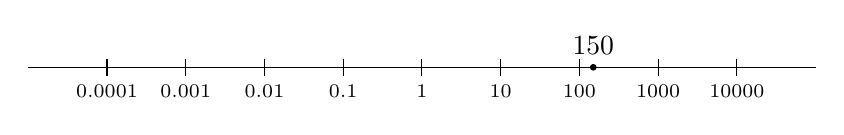
\begin{tikzpicture}
    \draw (-5,0) -- (5,0);
    \def\drawhorizontalmark#1#2{\draw (#1, 3pt) -- (#1,-3pt) node
      [below] {$\scriptstyle#2$};}
    \drawhorizontalmark{-4}{\numprint{0.0001}}%
    \drawhorizontalmark{-3}{\numprint{0.001}}%
    \drawhorizontalmark{-2}{\numprint{0.01}}%
    \drawhorizontalmark{-1}{\numprint{0.1}}%
    \drawhorizontalmark{0}{\numprint{1}}
    \drawhorizontalmark{1}{\numprint{10}}%
    \drawhorizontalmark{2}{\numprint{100}}
    \drawhorizontalmark{3}{\numprint{1000}}%
    \drawhorizontalmark{4}{\numprint{10000}}%
    \draw[fill](2.17609126, 0) circle (1pt) node [above=+1pt] {$150$};
  \end{tikzpicture}
\end{center}
ce qu'on comprend en \og prenant le logarithme (en base $10$) de tout
cela~:\fg{}
\begin{center}
  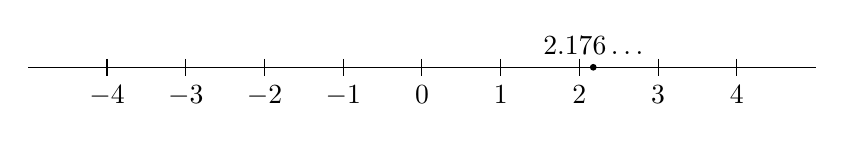
\begin{tikzpicture}
    \draw (-5,0) -- (5,0);
    \def\drawhorizontalmark#1#2{\draw (#1, 3pt) -- (#1,-3pt) node
      [below] {$#2$};}
\foreach \x in {-4, ..., 4} \drawhorizontalmark{\x}{\x};
\draw[fill] (2.17609126, 0) circle (1pt) node [above=+1pt] {$\numprint{2.176}\dots$};
  \end{tikzpicture}
\end{center}
Cette seconde droite graduée est liée à la première de la manière suivante :
\begin{center}
$10^{-4}$ = \numprint{0.0001}, $10^{-3}$ = \numprint{0.001}, \dots, $10^{3}$ = \numprint{1000}, $10^{4}$ = \numprint{10000},
\end{center}
et bien évidemment : $10^{\numprint{2.176}} = 150$.
% \mycomment{26.64\\
%   27.73\\
%   26.02\\
%   28.16\\
%   27.78\\
%   27.58\\
%   27.85\\
%   27.19}
\end{frame}
\begin{frame}{Arcsinus}
La fonction $\sin : \intercc{-\dfrac{\pi}{2}, \dfrac{\pi}{2}} \to \intercc*{-1,1}$
possède une réciproque notée :
\begin{equation*}
\arcsin : \intercc*{-1,1} \to \intercc*{-\dfrac{\pi}{2},\dfrac{\pi}{2}}
\end{equation*}

\begin{figure}[ht!]
\centering
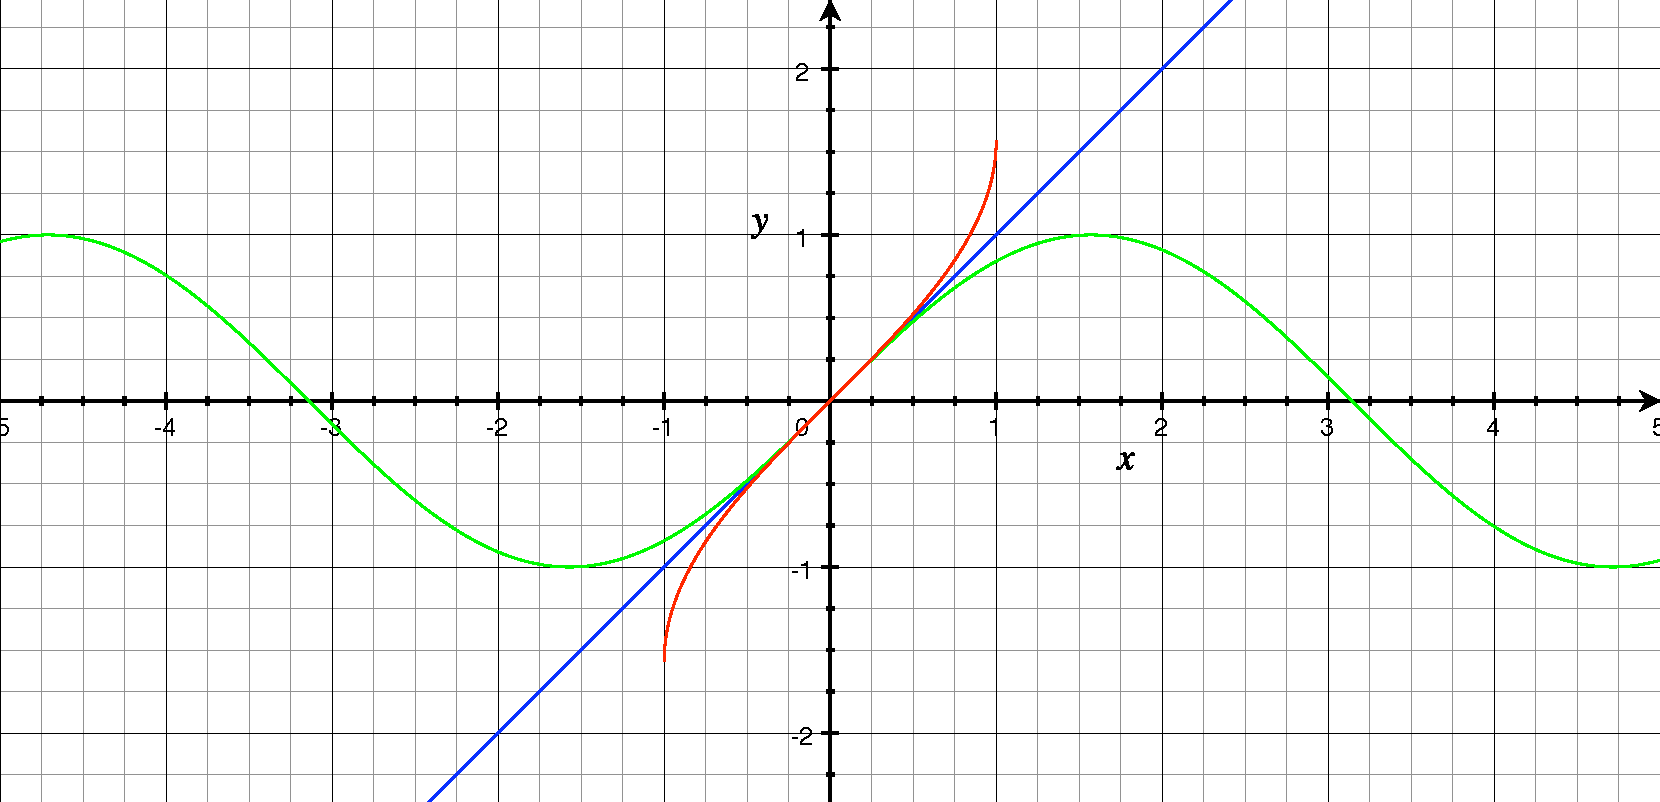
\includegraphics[width=\textwidth]{sin-arcsin.pdf}
\caption{Graphes de $\sin$ et $\arcsin$}
\end{figure}
\end{frame}
\course{6}
\renewcommand{\vec}[1]{\fleche{#1}}% FIXME: utiliser dès le début
\subsection{Fonctions trigonométriques réciproques}
\begin{frame}{Réciproque}
  \begin{definition}
    Une fonction $f\colon A \vers B$ est \Defn{inversible} si il existe une fonction $g\colon B \vers A$ telle que
    \begin{equation*}
      g(f(x)) = x\quad \forall x \in A \qquad\text{et}\qquad f(g(y)) = y \quad\forall y  \in B.
    \end{equation*}
    La fonction $g$ est appelée l'\Defn{inverse} ou la \Defn{fonction réciproque} de $f$, et se note $f^{-1}$.
  \end{definition}\pause

\begin{remark*}
  Attention à ne pas confondre $f^{-1} (x)$ avec $f(x)^{-1} \pardef 1/f(x)$~! Par exemple, les fonctions
  \begin{equation*}
    f : \RR_0 \vers \RR_0 : x\mapsto x \quad\text{et}\quad g : \RR_0 \vers
    \RR_0 : x \mapsto \frac1x
  \end{equation*}
  vérifient $f(x)^{-1} = g(x)$ pour tout $x \in \RR_0$, par contre
  $f^{-1} = f$ et $g^{-1} = g$ (exercice facile).
\end{remark*}
\end{frame}
\begin{frame}
\begin{proposition}
  \begin{enumerate}
  \item Une fonction est inversible si et seulement si c'est une bijection.
  \item Si $g$ est l'inverse de $f$, alors $f$ est l'inverse de $g$. En d'autres termes,
    \begin{equation*}
      {\left(f^{-1}\right)}^{-1} = f.
    \end{equation*}
  \end{enumerate}
\end{proposition}
\begin{proof}
  Si \(f\) est inversible (d'inverse \(g\))\pause, alors \(f\) est
  \begin{itemize}[<+->]
  \item injective car \(f(x) = f(y)\) implique \(x = g(f(x)) = g(f(y)) = y\).
  \item surjective car si \(z \in B\), alors \(g(z)\) est un antécédent de z.
  \end{itemize}\pause
  Si \(f\) est bijective, alors pour tout \(z\in B\) il existe un (surjectivité) unique (injectivité) antécédent.
\end{proof}
\end{frame}
\begin{frame}{Graphe de la réciproque}

Si $f : A \to B$ est bijective, alors le graphe de sa réciproque $f^{-1} : B \to A$ peut s'obtenir en prenant l'image du graphe de $f$ par une symétrie bilatérale d'axe $x = y$. En effet,
\begin{equation*}
\Gamma_{f^{-1}} = \{(y,f^{-1}(y)) \in \RR^2 \telque y \in B\}
= \{(f(x),x) \in \RR^2 \telque x \in A\}
\end{equation*} 
\end{frame}
\begin{frame}{Arcsinus}
La fonction $\sin : \intercc*{-\dfrac{\pi}{2}, \dfrac{\pi}{2}} \to \intercc*{-1,1}$
possède une réciproque notée :
\begin{equation*}
\arcsin : \intercc*{-1,1} \to \intercc*{-\dfrac{\pi}{2},\dfrac{\pi}{2}}
\end{equation*}

\begin{center}
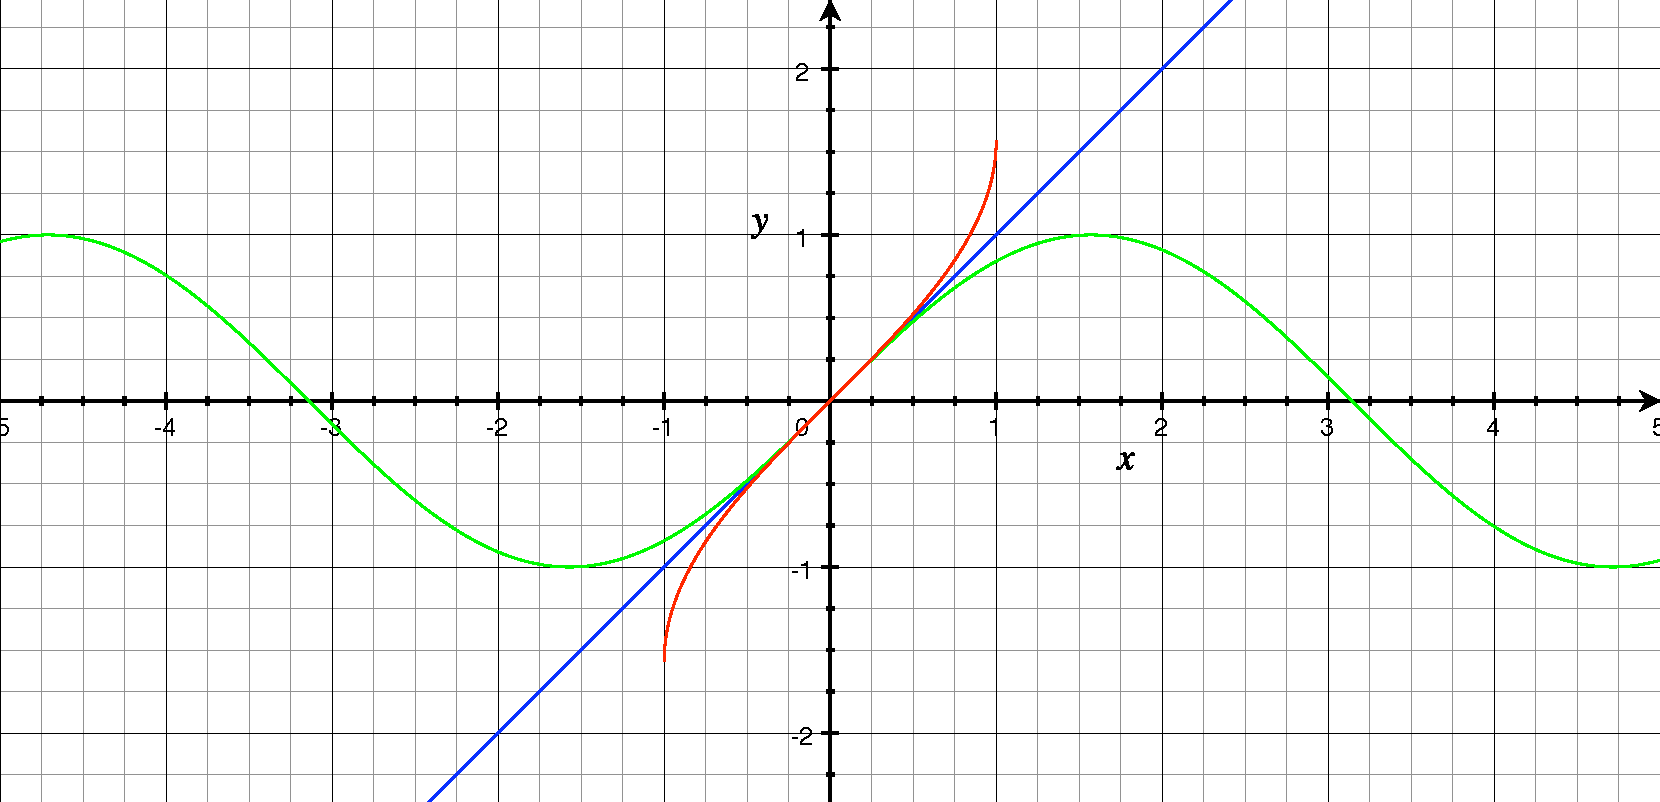
\includegraphics[width=\textwidth]{sin-arcsin.pdf}
\end{center}

\end{frame}
\begin{frame}{Arccosinus}
La réciproque de $\cos : \intercc*{0,\pi} \to \intercc*{-1,1}$ est
\begin{equation*}
\arccos : \intercc*{-1,1} \to \intercc*{0,\pi}
\end{equation*}

\begin{center}
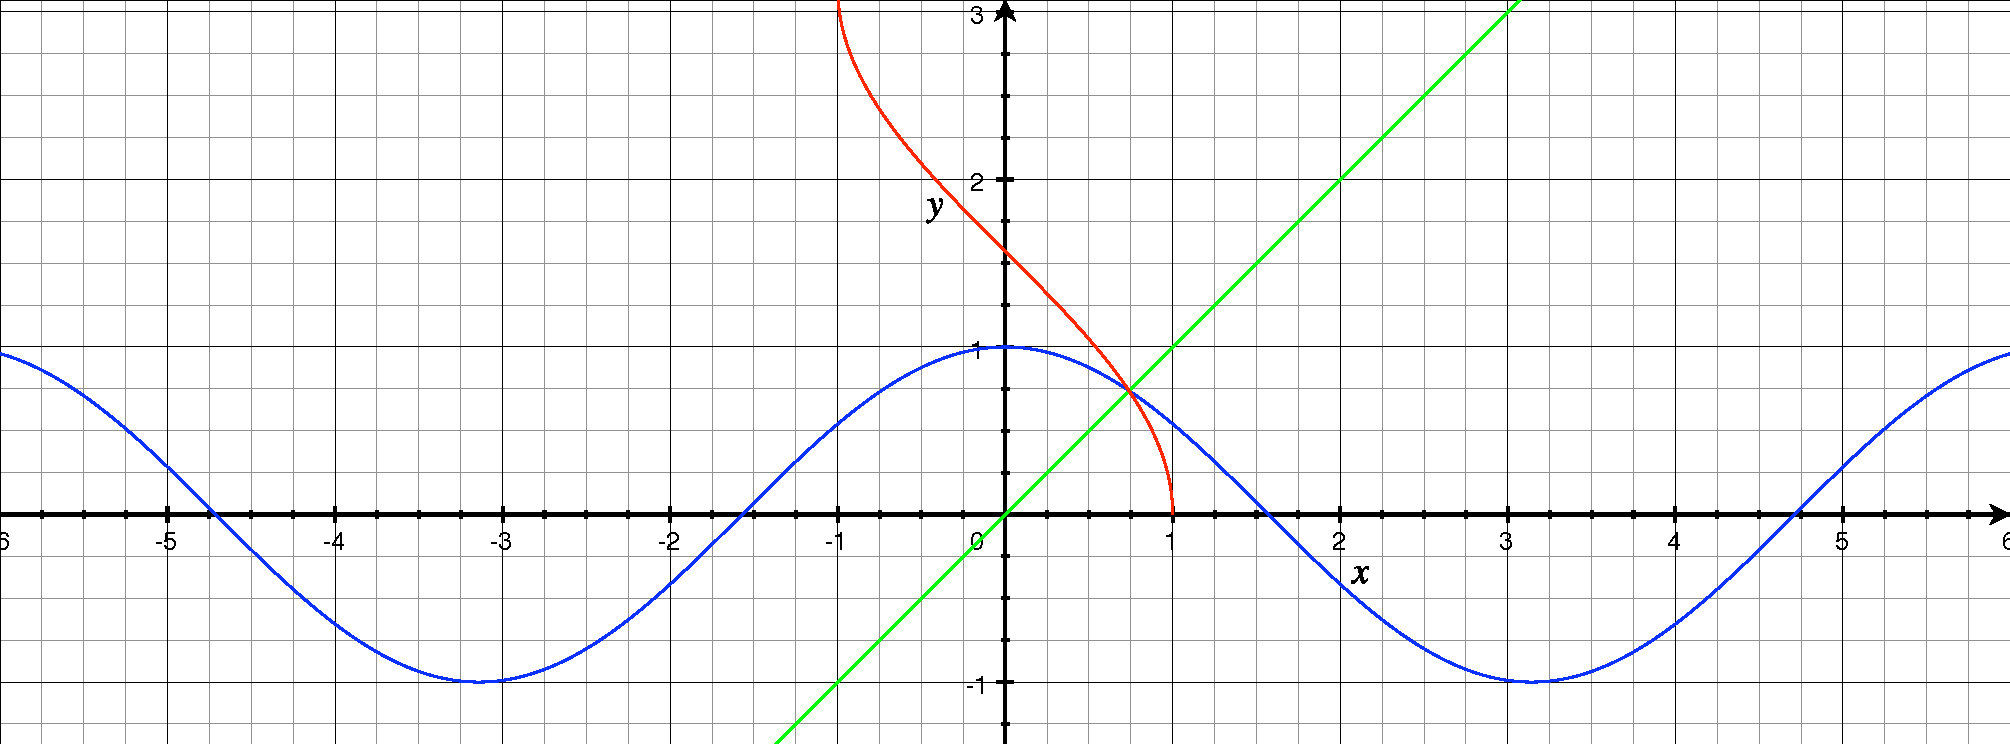
\includegraphics[width=\textwidth]{cos-arccos.pdf}
\end{center}

\end{frame}
\begin{frame}{Arctangente}
La réciproque de $\tg : \interoo*{-\dfrac{\pi}{2}, \dfrac{\pi}{2}} \to \interoo*{-\infty,
\infty}$ est 
\begin{equation*}
\arctg : \interoo*{-\infty, \infty} \to \interoo*{-\dfrac{\pi}{2},\dfrac{\pi}{2}}
\end{equation*}

\begin{center}
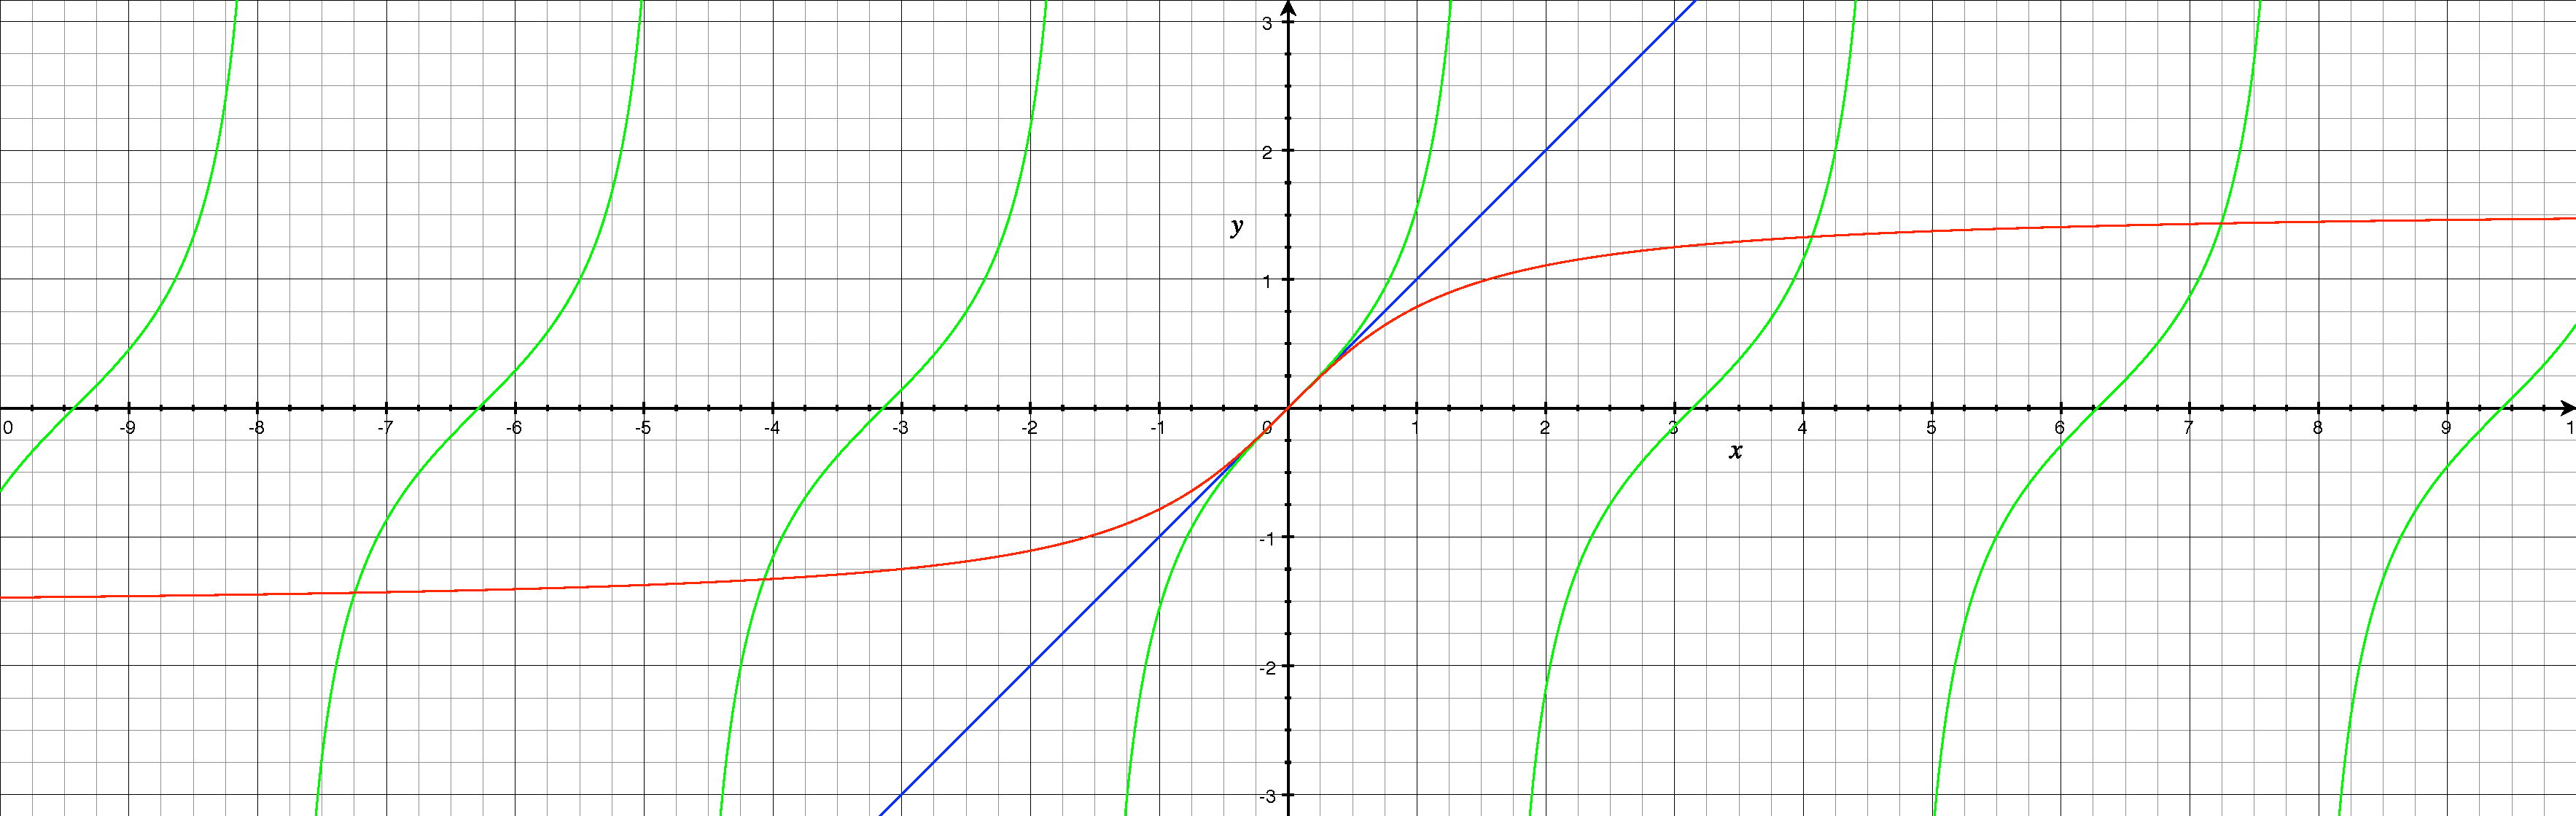
\includegraphics[width=\textwidth]{tan-arctan.pdf}
\end{center}

On peut aussi définir la réciproque de $\cotg : \interoo*{0,\pi} \to \interoo*{-\infty,\infty}$.
\end{frame}

%\subsection{Loi des sinus}
\begin{frame}{Loi des sinus}
  %% FIXME move earlier
  \begin{minipage}{0.49\linewidth}
  Soit un triangle de sommets \(A,B,C\) tel que représenté ci-contre, alors :
  \begin{equation*}
    \frac{\sin \hat A}{a} = \frac{\sin\hat B}{b} = \frac{\sin\hat C}{c}
  \end{equation*}
\end{minipage}
\begin{minipage}{0.49\linewidth}
  \includegraphics{triangleqcq}
\end{minipage}
  \begin{proof}\pause % FIXME: intégrer au syllabus
    Prouvons l'une de ces égalités :

    Notons \(h\) la hauteur issue de \(B\). Alors d'une part \(\sin \hat{C} = \frac{h}{a}\) et d'autre part \(\sin \hat{A} = \frac{h}{c}\), ceci prouve
    \begin{equation*}
      \frac{\sin \hat A}{a} =  \frac{\sin\hat C}{c}
    \end{equation*}
  \end{proof}
\end{frame}

%\subsection{Loi des cosinus}
\begin{frame}{Loi des cosinus}
\vspace*{-1\baselineskip}
  \begin{minipage}{0.59\linewidth}
  Soit un triangle de sommets \(A,B,C\) tel que représenté ci-contre, alors :
  \begin{equation*}
    c^{2} = a^{2} + b^{2} - 2 a b \cos \hat{C}
  \end{equation*}
  Ceci est un théorème de Pythagore généralisé
\end{minipage}
\begin{minipage}{0.39\linewidth}
  \includegraphics{triangleqcq}
\end{minipage}
\vspace{-1.3\baselineskip}
\begin{proof}\pause % FIXME: intégrer au syllabus
    Notons \(\vec{AC} = \point{C} - \point{A}\) pour le vecteur de \(\point{A}\) à \(\point{C}\), etc. et développons \(c^{2}\) grâce au produit scalaire :
    \begin{align*}
      \uncover<+->{c^{2} &= \norme{\vec{AB}}^{2} = \norme{\vec{AC} + \vec{CB}}^{2}}
      \uncover<+->{= \norme{\vec{AC}}^{2} + \norme{\vec{CB}}^{2} + 2 \scalprod{\vec{AC}}{\vec{CB}} \\}
      \uncover<+->{&= \norme{\vec{AC}}^{2} + \norme{\vec{CB}}^{2} + 2 \norme{\vec{AC}} \norme{\vec{CB}} \cos(\pi - \hat{C})\\}
      \uncover<+->{&= \norme{\vec{AC}}^{2} + \norme{\vec{CB}}^{2} - 2 \norme{\vec{AC}} \norme{\vec{CB}} \cos(\hat{C})}
    \end{align*}\pause
  Attention, l'angle entre \(\vec{AC}\) et $\vec{CB}$ est \(\pi - \hat{C}\) car ils n'ont pas le même point base sur l'image. 
  \end{proof}
\end{frame}


\begin{frame}{Diagrammes de Venn} % FIXME: intégrer au syllabus
Si  \(A\) et \(B\) sont des ensembles, on définit les trois opérations :
  \begin{description}
  \item[Intersection] $A \cap B = \set{ x \telque \text{\(x \in A\) et \(x \in B\)}}$
  \item[Union] $A \cup B = \set{ x \telque \text{\(x \in A\) ou \(x \in B\)}}$
  \item[Différence] $A \setminus B = \set{ x \telque \text{\(x \in A\) et \(x \notin B\)}}$
  \end{description}\pause

On peut représenter les opérations sur des diagrammes appelés diagrames de Venn.
\end{frame}

\begin{frame}
  \begin{exercise} % FIXME: intégrer au syllabus
    Voici deux diagrammes de Venn :
    \begin{center}
      \raisebox{-.5\height}{\begin{venndiagram2sets}[shade=red] \fillACapB
        \end{venndiagram2sets}} \raisebox{-.5\height}{\begin{venndiagram3sets}[shade=green] \fillOnlyA
        \end{venndiagram3sets}}
    \end{center}
    Que représentent-ils ?
  \end{exercise}\pause{}

  Réponse : \(A \cap B\) et \(A\setminus (B\cup C)\)
\end{frame}

\section{Questions qu'on pourrait poser à l'examen}
\begin{frame} % FIXME: intégrer au syllabus
\begin{itemize}
\item Prouver (telle formule) par récurrence.
\item Qu'est ce que la transitivité (pour les inégalités) ?
\item Démontrer : si \(a < b\) et \(c < d\), alors \(a + c < b + d\).
\item Écrire \(\interco{-2,4}\cup \interoc{-5,1}\) sous forme d'intervalle.
\item Définir : l'intérieur d'un ensemble.
\item Les ensembles suivants sont ils ouverts ? fermés ? (suivi d'une liste d'ensembles)
\item De combien de manière peut on disposer \(k\) billes identiques dans deux urnes ?
\item Définir : racine carrée de \(x\).
\item Définir : fonction croissante (donner un exemple et un contre-exemple)
\item Définir le logarithme d'un nombre \(a\) en base \(b\). À quelles conditions sur \(a\) et \(b\) ce logarithme existe-t-il ?
\item Donner et prouver la formule donnant le cosinus d'une somme.
\item Donner et prouver la formule de Cauchy-Schwarz.
\item etc.
\end{itemize}
\end{frame}

\section{Exercices}
\begin{frame} % FIXME: intégrer au syllabus
\begin{itemize}
\item Quelle est l'équation de la droite du plan qui passe par $(2,-3)$ et qui 
est parall\`ele \`a la droite passant par $(4,1)$ et $(-2,2)$ ?
\item \(\arccos(\frac{\sqrt{3}}{2})\), \(\arcsin(\frac{\sqrt{3}}{2})\), \(\arctan(1)\)
\item \(\cos(\arcsin(x))\)
\item Quelle est l'équation de la perpendiculaire \`a la droite d'équation 
$2x-3y-4=0$, qui passe par le point $(3,-2)$ ?
\item Pour quelles valeurs du nombre naturel $m$ avons-nous
$
\left(\frac{1}{2}\right)^m < 10^{-5} \quad ?
$
\item (difficile) Quel est le nombre de solutions enti\`eres $(x_1,x_2,\ldots, x_n)$ de l'équation $x_1+x_2+\cdots +x_n=m$, o\`u de plus $x_i>0$ pour $i=1,2,\ldots n$~?
Ici $m$ est un naturel donné.
\item En sommant les nombres sur les premières lignes du triangle de Pascal, intuitez la valeur de \(\sum_{k=0}^{n} \binom{n}{k}\) pour tout \(n\) fixé. Démontrez cela en utilisant le binôme de Newton pour \((1+1)^n\).
\item Trouver les équations des droites tangentes au cercle d'équation 
$x^2+y^2-4x-2y-3=0$ et parall\`eles \`a la droite d'équation $x+y=0$.
\end{itemize}
\end{frame}
\section{Réponses} % FIXME: intégrer au syllabus (toute la section, si on met les exos.)
\begin{frame}
  \begin{enonce}
    En sommant les nombres sur les premières lignes du triangle de Pascal, intuitez la valeur de \(\sum_{k=0}^{n} \binom{n}{k}\) pour tout \(n\) fixé. Démontrez cela en utilisant le binôme de Newton pour \((1+1)^n\).
  \end{enonce}

  \begin{answer}
    \begin{minipage}{0.49\linewidth}
    \fbox{\includegraphics[width=.8\linewidth]{pascal2}} % triangle isocèle
  \end{minipage}
  \begin{minipage}{0.49\linewidth}
  \begin{align*}
    2^{n}  &= (1+1)^{n}\\
           &=   \sum_{k=0}^{n} \binom{n}{k} 1^{k} 1^{n-k} \\
    &= \sum_{k=0}^{n} \binom{n}{k}
  \end{align*}
\end{minipage}
\end{answer}
\end{frame}
\begin{frame}
  \begin{enonce}
  (difficile) Quel est le nombre de solutions enti\`eres $(x_1,x_2,\ldots, x_n)$ de l'équation $x_1+x_2+\cdots +x_n=m$, o\`u de plus $x_i>0$ pour $i=1,2,\ldots n$~? Ici $m$ est un naturel donné.
\end{enonce}

\begin{answer}
On place \(m\) billes et on se demande où il faut les \og séparer\fg{}. On a \(\binom{m-1}{n-1}\) choix pour les séparations.
\end{answer}
\end{frame}
\begin{frame}
  \begin{enonce}
  Pour quelles valeurs du nombre naturel $m$ avons-nous $\left(\frac{1}{2}\right)^m < 10^{-5}$ ?
\end{enonce}

\begin{answer}
 On veut \(2^{m} > 10^{5}\). Ok pour \(m \geq 17\) .
\end{answer}
\end{frame}
\begin{frame}
  \begin{enonce}
  Quelle est l'équation de la perpendiculaire \`a la droite d'équation $2x-3y-4=0$, qui passe par le point $(3,-2)$ ?
\end{enonce}

\begin{answer}
Réponse : \(3(x-3) + 2(y+2) = 0\)
\end{answer}
\end{frame}
\begin{frame}
  \begin{enonce}
\(\cos(\arcsin(x))\)
\end{enonce}
\begin{answer}
$\arcsin$ prend ses valeurs dans \(\intercc{-\pi/2, \pi/2}\). Le cosinus y est toujours positif, dès lors
\begin{equation*}
  \cos(\arcsin(x)) = \sqrt{1 - \sin^{2}(\arcsin(x))} = \sqrt{1 - x^{2}}
\end{equation*}
pour \(x \in \intercc{-1,1}\)
\end{answer}
\end{frame}
\begin{frame}
  \begin{enonce}
    \(\arctan(1)\)
  \end{enonce}

  \begin{answer}
\(\pi/4\)
\end{answer}
\end{frame}
\begin{frame}
  \begin{enonce}
\(\arcsin(\frac{\sqrt{3}}{2})\)
\end{enonce}

\begin{answer}
\(\pi/3\)
\end{answer}
\end{frame}
\begin{frame}
  \begin{enonce}
    \(\arccos(\frac{\sqrt{3}}{2})\)
  \end{enonce}

  \begin{answer}
 \(\pi/6\)
\end{answer}

\end{frame}
\begin{frame}
  \begin{enonce}
Quelle est l'équation de la droite du plan qui passe par $(2,-3)$ et qui est parall\`ele \`a la droite passant par $(4,1)$ et $(-2,2)$ ?
\end{enonce}

\begin{answer}
Vecteur directeur : \((4,1)- (-2,2) = (6,-1)\). Vecteur normal : \((1,6)\). Équation
\begin{equation*}
  (x-2) + 6 (y+3) = 0
\end{equation*}
\end{answer}
\end{frame}
\begin{frame}
  \begin{enonce}
Trouver les équations des droites tangentes au cercle d'équation $x^2+y^2-4x-2y-3=0$ et parall\`eles \`a la droite d'équation $x+y=0$.
\end{enonce}

\begin{answer}
le cercle a pour équation \((x-2)^{2} + (y - 1)^{2} = 8\). Le rayon est perpendiculaire à la tangente, donc le rayon va du centre \((2,1)\) à \((2,1) \pm 2 \sqrt{2} (\sqrt{2}/2,\sqrt{2}/2) = (2,1) \pm (2,2)\) càd \((4,3)\) et \((0,-1)\). Les équations sont donc :

\((x-4) + (y - 3) = 0\)


\(x + y + 1 = 0\)
\end{answer}
\end{frame}
\course{7}
%%
\section{Fonctions réelles}
\begin{frame} % FIXME: intégrer au syllabus
  \frametitle{Motivation}
  \begin{example}
    \begin{minipage}{0.49\linewidth}
      Voici quelques fonctions de \(\RR\) dans \(\RR\), qui à \(x\) associent :
      \begin{itemize}[<+->]
      \item \(1\)
      \item \(x^{2}\)
      \item \(\exp{x}\)
      \item \(0\) si \(x < 0\), \(x^{3}\) sinon.
      \item \(\abs{x}\)
      \item \(1\) si \(x \in \QQ\) et \(0\) sinon.
      \end{itemize}\pause
      et voici les graphes de ces fonctions (sauf la dernière.)
    \end{minipage}\pause
    \begin{minipage}{0.49\linewidth}
      \begin{center}
        \includegraphics[width=4.3cm]{graphes-de-fctsreelles}
      \end{center}
    \end{minipage}
  \end{example}
\end{frame}
\begin{frame}% FIXME: intégrer au syllabus
  \frametitle{Motivation, suite}
  Certaines fonctions sont plus agréables que d'autres.
  \begin{itemize}[<+->]
  \item Comment les caractériser ?
  \item Comment les trouver ?
  \item Quelles sont leurs propriétés ?
  \end{itemize}\pause
  Nous décrirons plusieurs classes de fonctions \og agréables\fg{} :
  \begin{itemize}[<+->]
  \item continue
  \item dérivable
  \item \(\Cclass^{\infty}\) (lire \og C infinie\fg{})
  \end{itemize}
\end{frame}

\section{Limites}

\begin{frame}{Distances}
  \begin{rappel}
    La distance entre deux réels quelconques $x$ et $y$ est $|x - y|$.
  \end{rappel}

  \begin{block}{}
  Si $\delta > 0$, demander $|x - y| < \delta$ revient donc à demander que la distance entre $x$ et $y$ soit inférieure à $\delta$.
\end{block}

\begin{block}{}
On a les équivalences suivantes~:
  \begin{equation*}
    |x - y| < \delta \iff x \in \interoo*{y-\delta,y+\delta} \iff y - \delta < x < y+\delta
  \end{equation*}
\end{block}

\end{frame}

\begin{frame}{Points adhérents}
  \begin{definition}
    Un réel $a$ est dit \Defn{adhérent} à un sous-ensemble $A$ de $\R$ si pour tout $\delta > 0$ il existe un point $x$ de $A$ tel que $|x - a| < \delta$.

    \pause On écrit aussi :
    \begin{equation}
      \forall \delta > 0, \exists x \in A : \abs{x-a} < \delta
    \end{equation}
  \end{definition}\pause

On note \(\adh A\) l'ensemble des points adhérents à \(A\).
\end{frame}

\begin{frame}% FIXME: intégrer au syllabus
  \begin{example}
    Les points adhérents à l'ensemble ... forment l'ensemble ... :
    \begin{equation*}
      \begin{array}{cc}
        \interoc{0,1} &\intercc{0,1}\\
        \interco{0,1} &\intercc{0,1}\\
        \intercc{0,1} &\intercc{0,1}\\
        \interoo{0,1} &\intercc{0,1}\\
        \RR & \RR\\
        \interoo{-\infty, 2} &       \interoc{-\infty, 2}\\
        \RR_0 & \RR\\
        \QQ & \RR\\
        \NN &\NN
      \end{array}
  \end{equation*}
  \end{example}
\end{frame}

\begin{frame}{Idée de limite}% FIXME: intégrer au syllabus
  Considérons la fonction \(f: \RR_0 \to \RR : x \mapsto \frac{\sin x}{x}\). \pause Son graphe~:
  \begin{center}
    \includegraphics{sinxsurx}
  \end{center}\pause
  La valeur \(f(0)\) n'a aucun sens car \(0\) n'est pas dans le domaine, car \(\frac{0}{0}\) n'a aucun sens.

  \pause Mais on a envie de dire \(f(0) = 1\).

  \pause À la place, on dira \(\limite x 0 f(x) = 1\), et on va définir cela rigoureusement.
\end{frame}

\begin{frame}{Idée de limite}% FIXME: intégrer au syllabus
  Considérons la fonction \(f: \RR_0 \to \RR : x \mapsto \sin(1/x)\). \pause Son graphe~:
  \begin{center}
    \includegraphics{sin1surx}
  \end{center}\pause
  La valeur \(f(0)\) n'a aucun sens car \(0\) n'est pas dans le domaine, car \(\frac{1}{0}\) n'a aucun sens.

  \pause Quelle valeur a-t-on envie que \(f(0)\) prenne ? Hmm...

  \pause À la place, on dira \(\limite x 0 f(x)\) n'existe pas.
\end{frame}
  

% \begin{frame}{Idée de limite, 2}
%   Considérons la fonction \(f : \RR\)

%   Son graphe, on se l'imagine comme suit (en bleu)~:
%   \begin{center}
%     \includegraphics{graphe-de-fct-car-de-Q}
%   \end{center}

%   où les deux lignes ne sont pas continues, mais \og trouées\fg{} :
%   \begin{itemize}
%   \item les points d'abcisse rationnelle sont en haut,
%   \item ceux d'abcisse irrationnelles sont à hauteur \(0\).
% \end{itemize}

%   Donc : quand on s'approche d'une valeur fixée de \(x\), on va de haut en bas perpétuellemet
% \end{frame}


\begin{frame}{Définition de limite}% FIXME: intégrer au syllabus
  \begin{definition}
    Soit $f : A \to B$ où $A, B \subseteq \mathbb R$ et soit $a$ un point adhérent à $A$.\pause{}

    Un nombre réel $L$ est la \Defn{limite de $f$ en $a$} si
    \begin{equation*}
      \forall \epsilon > 0, \exists \delta > 0 : \forall x \in A, \abs{x-a} < \delta \Rightarrow \abs{f(x)-L} < \epsilon.
    \end{equation*}
  \end{definition}\pause

  Si $L$ est la limite de $f$ en $a$, on écrit
  \begin{equation}
    \lim_{x \to a} f(x) = L.
  \end{equation}
  On dit aussi que la limite (de \(f\) en \(a\)) existe et vaut \(L\).\pause

  \begin{definition}
    S'il n'existe pas de $L \in \R$ tel que $L$ est la limite de $f$ en $a$ est $L$, on dit que la limite de $f$ en $a$ n'existe pas (dans $\R$).
  \end{definition}
\end{frame}
 
\begin{frame}
  \begin{definition}
    Ré-écrivons la définition
    \begin{equation*}
      \forall \epsilon > 0, \exists \delta > 0 : \forall x \in A, \abs{x-a} < \delta \Rightarrow \abs{f(x)-L} < \epsilon.
    \end{equation*}
  \end{definition}\pause

  \begin{remark}
    L'ordre des quantificateurs \og pour tout\fg{} et \og il existe\fg{} est importante. On choisit d'\emph{abord} une précision $\epsilon$ et puis \emph{ensuite} un rayon $\delta$ adapté à cette précision. Typiquement, au plus la précision $\epsilon$ est petite, au plus il faudra choisir le rayon $\delta$ petit.
  \end{remark}
\end{frame}

\begin{frame}{Exemple}
    Montrons que
    \begin{equation*}
      \lim_{x \to 0} \sqrt{x} = 0
    \end{equation*}
    en utilisant la définition.

    \begin{question}
      Comment doit-on choisir $\delta = \delta(\epsilon)$ pour que $|x - 0| < \delta$ (et \(x \geq 0\)) garantisse $|\sqrt{x}-0| < \epsilon$~?
    \end{question}
    \begin{answer}
      Il suffit de prendre $\delta = \epsilon^2$, car
      \begin{equation*}
        |x - 0| < \epsilon^2 \Longrightarrow 
        x < \epsilon^2 \Longrightarrow
        \sqrt{x} < \epsilon \Longrightarrow
        |\sqrt{x} - 0| < \epsilon
      \end{equation*}
      pour $x \geqslant 0$.
    \end{answer}

    Pour garantir une précision de $\epsilon = 0,01 = 10^{-2}$ on peut prendre $\delta = \epsilon^2 = 10^{-4} = 0,0001$.
\end{frame}

\begin{frame}{Unicité}
  Parler de \og la limite\fg{} n'est raisonnable que si la limite est unique.\pause \begin{proposition}Si \(L_{1}\) et \(L_{2}\) sont deux nombres vérifiant la définition de \og limite de \(f\) en \(a\), alors \(L_{1} = L_{2}\)
  \end{proposition}
\end{frame}
\begin{frame}% FIXME: intégrer au syllabus
  \begin{proof}Supposons \(L_{1} > L_{2}\) (le cas inverse est semblable). Dès lors \(\epsilon = \paren*{L_{1} - L_{2}}/2 > 0\).

    Alors il existe \(\delta_{1} > 0\) tel que
    \begin{equation*}
      \forall x \in A, \abs{x-a} < \delta_{1} \Rightarrow \abs{f(x)-L_{1}} < \epsilon.
    \end{equation*}\pause
    et il existe \(\delta_{2} > 0\) tel que
    \begin{equation*}
      \forall x \in A, \abs{x-a} < \delta_{2} \Rightarrow \abs{f(x)-L_{2}} < \epsilon.
    \end{equation*}
    et il existe \(x \in A\) avec \(\abs{x-a} < \min\set{\delta_{1},\delta_{2}}\).

    Pour ce \(x\), on a~:
    \begin{align*}
      - (L_{1} - L_{2}) /2 &< f(x) - L_{1} &      f(x) - L_{2} &< (L_{1} - L_{2}) /2
    \end{align*}
    c'est-à-dire~:
    \begin{align*}
      (L_{1} + L_{2}) /2 < f(x) < (L_{1} + L_{2}) /2
    \end{align*}
    d'où une contradiction !
  \end{proof}
\end{frame}
\begin{frame}{Limites restreintes}
  \begin{definition}
    Si on ne s'intéresse qu'à certaines valeurs de \(x\), on écrira
    \begin{equation*}
      \limite[\text{condition sur \(x\)}] x a f(x) = L
    \end{equation*}
    lorsque
    \begin{equation*}
      \forall \epsilon > 0, \exists \delta > 0~: \forall x \in A,
      \begin{cases}
        \abs{x-a} < \delta, \text{ et}\\
        \text{condition sur \(x\)}
      \end{cases}
      \Longrightarrow \abs{f(x)-L} < \epsilon.
    \end{equation*}
    \begin{example}Les limites \og épointées\fg{}, \og à droite\fg{} et \og à gauche\fg{} sont les suivantes :
      \begin{equation*}
        \lim_{\substack{x \to a\\ x \neq a}} f(x)
        \qquad,\qquad
        \lim_{\substack{x \to a\\ x > a}} f(x)
        \qquad \textrm{et} \qquad
        \lim_{\substack{x \to a\\ x < a}} f(x)
      \end{equation*}
    \end{example}
  \end{definition}
\end{frame}

\begin{frame}{Limite épointée, limites latérales}
  \begin{example}
    La limite lorsque \(x \to 0\) de \(\abs{x}/x\) n'existe pas, mais
    \begin{align*}
      \limite [x<0] x 0 \frac{\abs{x}}{x} &= -1 &       \limite [x>0] x 0 \frac{\abs{x}}{x} &= 1
    \end{align*}

    \begin{center}
      \includegraphics{graphe-absssurx}% FIXME: intégrer au syllabus
    \end{center}
  \end{example}
\end{frame}

\begin{frame}{Lien entre les limites}% FIXME: intégrer au syllabus
  \begin{proposition}
    Soit \(f : A \to \RR\) et \(a \in A\). Si \(\limite{x}{a} f(x)\) existe, alors elle vaut \(f(a)\).
  \end{proposition}
  \begin{proof}\pause
    Supposons que la limite vaut \(L\) :
    \begin{equation*}
      \forall \epsilon > 0, \exists \delta > 0 : \forall x \in A, \abs{x-a} < \delta \Rightarrow \abs{f(x)-L} < \epsilon.
    \end{equation*}
    Comme \(a \in A\), on peut prendre \(x = a\). Comme \(\abs{0 - 0} < \delta\) est toujours vrai, on a forcément \(\abs{f(a) - L} < \epsilon\). Pour tout \(\epsilon > 0\) ! Donc \(f(a) = L\).
  \end{proof}\pause
  \begin{remark}
    La notion de limite intéressante est donc celle de limite épointée, où on enlève \(a\) du domaine.
  \end{remark}
\end{frame}
\begin{frame}{Lien entre les limites}% FIXME: intégrer au syllabus
\begin{proposition}
    Lorsque \(a \in A\), \(\limite{x}{a} f(x)\) existe si et seulement si la limite épointée existe et vaut \(f(a)\).
  \end{proposition}\pause{}
  \begin{proposition}\label{limites épointées et latérales}
    $\displaystyle\lim_{\substack{x \to a\\ x \neq a}} f(x)$ existe si et seulement si $\displaystyle\lim_{\substack{x \to a\\ x > a}} f(x)$ et $\displaystyle\lim_{\substack{x \to a\\ x < a}} f(x)$ existent et sont \emph{égales}.
  \end{proposition}
\end{frame}

\section{Limites infinies, limites à l'infini}
\begin{frame}
  \begin{minipage}{0.49\linewidth}
 Parfois on voudrait
 \begin{itemize}
 \item écrire \(L = \pm \infty\)
 \item étudier les cas \(a = \pm \infty\)
 \end{itemize}
 \begin{remark}<2->
   La définition de limite est essentiellement :
   \begin{center}
     Si $x \approx a$ alors \(f(x)\approx L\).
   \end{center}

   Il suffira d'exprimer ces conditions différemment lorsque l'infini et impliqué.
 \end{remark}
\end{minipage}
\begin{minipage}{0.49\linewidth}
  \begin{center}
    \includegraphics{graphe-1surx}% FIXME: intégrer au syllabus
  \end{center}
\end{minipage}
\end{frame}

\begin{frame}% FIXME: intégrer au syllabus
  \begin{remark*}
    Chaque utilisation du symbole \(\infty\) s'accompagne d'une définition ! L'infini n'intervient pas comme un cas particulier de ce qu'on a vu précédemment.
  \end{remark*}

  \begin{definition}
    Soit \(f : A \to \RR\) une fonction réelle et \(a\) adhérent à \(A\).

    On dit que \(f(x)\) tend vers \(-\infty\) pour \(x\) tendant vers \(a\) si
    \begin{equation*}
      \forall M > 0, \exists \delta > 0 : \forall x \in A, \abs{x-a}<\delta \Rightarrow f(x) < -M
    \end{equation*}
    on note cette situation
    \begin{equation*}
      \limite x a f(x) = -\infty
    \end{equation*}
  \end{definition}
\end{frame}
\begin{frame}% FIXME: intégrer au syllabus
  \begin{definition}
    Soit \(f : A \to \RR\) une fonction réelle dont le domaine n'est pas majoré. On dit que \(f(x)\) tend vers \(-\infty\) pour \(x\) tendant vers \(+\infty\) si
    \begin{equation*}
      \forall M > 0, \exists N > 0 : \forall x \in A, x > N \Rightarrow f(x) < -M
    \end{equation*}
    on note cette situation
    \begin{equation*}
      \limite x \infty f(x) = -\infty
    \end{equation*}
  \end{definition}
  \begin{remark}
    Les autres cas de limite infinie / à l'infini s'approchent de la même fa\c{c}on.
  \end{remark}
\end{frame}

\section{Limites et opérations}
\begin{frame}
  \begin{proposition}
    Si les deux limites, $\displaystyle{\lim_{x \to a} f(x)}$ et $\displaystyle{\lim_{x \to a} g(x)}$ existent dans $\mathbb R$, alors\pause{} $\displaystyle{\lim_{x \to a} \left[f(x)+g(x)\right]}$, $\displaystyle{\lim_{x \to a} cf(x)}$, $\displaystyle{\lim_{x \to a} \left[f(x)-g(x)\right]}$ et $\displaystyle{\lim_{x \to a} f(x)g(x)}$ existent aussi\pause{} et on a
    \begin{align*}
      \lim_{x \to a} \left[f(x)+g(x)\right] &= \lim_{x \to a} f(x) +
                                              \lim_{x \to a} g(x)\\
      \lim_{x \to a} cf(x) &= c \lim_{x \to a} f(x), \forall c \in \R\\
      \lim_{x \to a} \left[ f(x) - g(x) \right] &= \lim_{x \to a} f(x) -
                                                  \lim_{x \to a} g(x)\\
      \lim_{x \to a} f(x) g(x) &= \lim_{x \to a} f(x) \lim_{x \to a} g(x)
    \end{align*}\pause
    Si, de plus $\displaystyle{\lim_{x \to a} g(x) \neq 0}$,\pause{} alors $\displaystyle{\lim_{x \to a} \dfrac{f(x)}{g(x)}}$ existe\pause{} et on a
    \begin{equation*}
      \lim_{x \to a} \frac{f(x)}{g(x)} = \frac{\lim_{x \to a}
          f(x)}{\lim_{x \to a} g(x)}
    \end{equation*}
  \end{proposition}
\end{frame}
\begin{frame}
  \begin{proposition}
    Enfin, si on a une fonction composée $g \circ f$ et si on sait que $\displaystyle\lim_{x \to a} f(x) = L$ et que $\displaystyle\lim_{y \to L} g(y)$ existe alors $\displaystyle\lim_{x \to a} g(f(x))$ existe et on a
    \begin{equation*}
      \lim_{x \to a} g(f(x)) = \lim_{y \to L} g(y)
    \end{equation*}
  \end{proposition}
\end{frame}
\begin{frame}
  \begin{example}% FIXME: intégrer au syllabus
    Supposons savoir que \(\sin x/x\) tend vers \(1\) en \(0\).

    Alors
    \begin{equation*}
      \limite x 0 \frac{\sin (3x)}{x} = 3 \limite x 0 \frac{\sin (3x)}{3x} = 3 \limite t 0 \frac{\sin t}{t} = 3
    \end{equation*}
  \end{example}
  \begin{remark}
    En d'autres termes, on peut poser \(t\) = fonction de \(x\), et remplacer tous les \(x\) par des \(t\), et considérer la limite pour \(t\).
  \end{remark}
\end{frame}
\begin{frame}% FIXME: intégrer au syllabus
  \begin{example}
    \begin{equation*}
      \limite x 1 \frac{\sin (x^{2}-1)}{(x^{2}-1)} =       \limite t 0 \frac{\sin t}{t} = 1
    \end{equation*}
  \end{example}
\end{frame}

\section{Règles étendues}
\label{sec:regles-etendues}
\begin{frame}
  \begin{proposition}
    Les règles de calcul précédentes restent valables, sans modification, si on prend $a = +\infty$ ou $a = -\infty$.
  \end{proposition}

  \begin{proposition}
    Lorsque les limites sont \(\pm\infty\), chacune des \og égalités\fg{} suivante est un résultat qui se démontre :
    \begin{align*}
      (+\infty) + (+\infty) &= +\infty\\
      (-\infty) + (-\infty) &=-\infty\\
      c \cdot (\pm \infty)&=
                            \begin{cases}
                              \pm \infty &\textrm{si } c > 0\\
                              \mp \infty &\textrm{si } c < 0 \text{ (! changement de signe.)}
                            \end{cases}\\
      \infty \cdot \infty&=\infty\\
      \infty \cdot (-\infty)&=-\infty\\
      (-\infty) \cdot (-\infty)&=\infty
    \end{align*}
  \end{proposition}
\end{frame}

\begin{frame}
  En particulier, les \og quantités\fg{} suivantes n'ont aucun sens a priori :
  \begin{equation*}
    \infty - \infty,\; 0 \cdot \infty,\; 1^{\infty},\; \infty^{0},\; \frac{0}{0} \;\textrm{et}\; \frac{\infty}{\infty}.
  \end{equation*}
  
  Ce sont des \Defn{formes indéterminées}.

  \begin{example}% FIXME: intégrer au syllabus
    \begin{equation*}
      \limite{x}{0} \frac{x^2 + x}{x^2 - x} = \frac{0}{0}
    \end{equation*}
    On ne peut pas appliquer la règle de calcul du quotient ! Il faut écrire :
    \begin{equation*}
      \limite{x}{0} \frac{x^2 + x}{x^2 - x} = \limite{x}{0} \frac{x + 1}{x - 1} = \frac{1}{-1} = -1
    \end{equation*}
  \end{example}
\end{frame}
\begin{frame}
  \begin{example}% FIXME: intégrer au syllabus
    \begin{equation*}
      \limite{x}{\infty} \frac{x^2 + x}{x^2 - x} = \frac{\infty+\infty}{\infty - \infty}
    \end{equation*}
    On ne peut pas appliquer la règle de calcul du quotient ! Il faut écrire :
    \begin{equation*}
      \limite{x}{\infty} \frac{1 + 1/x}{1 - 1/x} 
      = \limite{x}{\infty} \frac{1 + 0}{1 - 0} = 1
    \end{equation*}
  \end{example}
\end{frame}
\begin{frame}
  \begin{proposition}
Pour le quotient, on pourra aussi prendre les conventions suivantes~:
\begin{align*}
  \frac{L}{0^+}&=
  \begin{cases}
    + \infty &\textrm{si } L > 0\\
    - \infty &\textrm{si } L < 0
  \end{cases}&
  \frac{L}{0^-}&=
  \begin{cases}
    - \infty &\textrm{si } L > 0\\
    + \infty &\textrm{si } L < 0
  \end{cases}\\
  \frac{\pm \infty}{0^+}&=\pm \infty&
  \frac{\pm \infty}{0^-}&=\mp \infty \text{ (changement de signe !)}
\end{align*}
\end{proposition}
\begin{remark}
  Une limite qui vaut $0^+$ signifie que $f(x) \to 0$ pour \(x \to a\) \texttt{et} $f(x) \geq 0$ pour $x \approx a$.
\end{remark}\pause
\begin{definition}
  Formellement, la condition $f(x) \geq 0$ pour $x \approx a$ se définit par : il existe \(\epsilon > 0\) tel que pour tout \(x\in A\) vérifiant \(\abs{x-a} < \epsilon\) on a \(f(x) \geq 0\).
\end{definition}
\end{frame}
\course{8}
\begin{frame}
  \begin{example}
    La fonction \(x \mapsto x\) a une limite nulle en \(0\). On peut cependant être plus précis et écrire~:
    \begin{align*}
      \limite[<] x 0 x &= 0^{-} & \limite[>] x 0 x &= 0^{+}.
    \end{align*}
    ce qui montre par les règles de calculs étendues :
    \begin{align*}
      \limite[<]{x}{0} \frac{1}{x} &= \frac{1}{0^{-}} = -\infty & \limite[>]{x}{0} \frac{1}{x} &= \infty.
    \end{align*}
  
    On pouvait aussi le démontrer via la définition. Par exemple pour la limite à droite : si \(K > 0\), on prend \(\delta\) un réel inférieur à \(1/K\), et alors pour tout \(x\) vérifiant \(\abs{x} < \delta\) et \(x > 0\) on a \(\frac{1}{x} > \frac{1}{\delta} = K\).
  \end{example}
\end{frame}

\begin{frame}{Petits et grand O}% FIXME: intégrer au syllabus
  \begin{definition}
    Soient \(f\) et \(g\) deux fonctions. Supposons qu'il existe \(r \in \RR\) et \(c \in \RR_{0}^{+}\) tels que pour tout \(x \in \interoo{r,+\infty}\) on a
    \begin{equation*}
      x \in \dom f, x \in \dom g \text{ et } \abs{f(x)} \leq c\cdot \abs{g(x)}
    \end{equation*}
    On dit alors \og $f$ est un $O(g)$\fg{} (prononcer \og \(f\) est un grand $O$ de $g$\fg{}).
\end{definition}\pause

\begin{remark}
  Cette notion indique essentiellement que \(f/g\) reste borné. Généralement on compare une fonction \(f\) intéressante à une fonction \(g\) bien connue. On dira aussi que l'\emph{ordre de grandeur} de \(f\) est inférieur à celui de \(g\).
\end{remark}
\end{frame}
\begin{frame}% FIXME: intégrer au syllabus
\begin{example}
  \begin{itemize}
  \item \(10x\) est \(O(x)\). En effet, si \(x > 0\), on a bien \(10x \leq c x\) (par exemple \(c = 10\) fonctionne).

  \item Inversement, \(x\) est \(O(10x)\) car \(x \leq c 10x\)

  \item \(\sin(x) + x^{2}\) est en \(O(x^{2})\) car \(\sin(x) + x^{2} \leq x^{2} + x^{2} = 2 x^{2}\) si \(x > 2\).

  \item \(x^{2}\) est \(O(x)\) mais \(x\) n'est pas \(O(x^{2})\).
\end{itemize}
\end{example}
\end{frame}
\begin{frame}% FIXME: intégrer au syllabus
\begin{proposition}
  Considérons la limite \(\limite{x}{\infty} \abs{\frac{f(x)}{g(x)}}\).
  \begin{itemize}
  \item Si elle existe dans \(\RR\), alors \(f(x)\) est \(O(g(x))\).
  \item Si elle est infinie, alors \(f(x)\) n'est pas \(O(g(x))\).
\end{itemize}
\end{proposition}
\begin{proof}
  Si la limite existe et vaut \(L\in \RR\), on prend \(\epsilon = 1\) dans la définition de limite. Ceci assure alors l'existence d'un \(N > 0\) tel que pour tout \(x \geq N\) on ait
  \begin{equation*}
    \abs{\abs{\frac{f(x)}{g(x)}} - \abs{L}} < 1
  \end{equation*}
  Dès lors \(\abs{\frac{f(x)}{g(x)}} < \abs{L} + 1\), ce qui prouve l'affirmation en prenant \(c = \abs{L} + 1\) (et \(r = N\)).

  Dans le second cas, quel que soit \(M > 0\), on sait qu'il existe \(N > 0\) tel  que pour \(x > N\), on a \(\abs{\frac{f(x)}{g(x)}} > M\). En particulier il ne peut pas exister de \(c\) vérifiant la définition de \og grand O\fg{}.
\end{proof}
\end{frame}
\begin{frame}% FIXME: intégrer au syllabus
  \begin{example}
    Pour tout réel \(A\) : \(A x^{n}\) est \(O(x^{k})\) si et seulement si \(n \leq k\). En d'autres termes : \(x^{n}\) est d'un ordre de grandeur inférieur à \(x^{k}\) si et seulement si \(n \leq k\).

    En effet le quotient de la proposition précédente vaut \(\abs{A x^{n-k}}\) :
    \begin{itemize}
    \item Si \(n \leq k\) alors l'exposant \(n-k\) est négatif ou nul, donc le quotient tend vers \(0\) ou \(\abs A\).
    \item Si \(n > k\), alors l'exposant est strictement positif et donc le quotient tend vers \(+\infty\).
    \end{itemize}
  \end{example}
\end{frame}

\begin{frame}% FIXME: intégrer au syllabus
  Une définition similaire est la suivante :
  \begin{definition}
    Lorsque \(\limite{x}{\infty} \abs{\frac{f(x)}{g(x)}} = 0\), on dit alors que \(f(x)\) est \(o(g(x))\).
  \end{definition}
  \begin{remark}
    \begin{itemize}[<+->]
    \item En particulier \(f(x)\) est en \(O(g(x))\) mais ceci est plus fort.
    \item On remarque que si \(g(x)\) tend vers \(0\) et \(f(x)\) est un \(o(g(x))\), alors \(f\) tend vers \(0\) plus vite que \(g\) !
    \item Les définitions de \(o\) et \(O\) tiennent encore lorsque \(x\) tend vers \(a \in \RR\) et vers \(-\infty\). Il faut alors préciser quelle est la limite pour \(x\) !
  \end{itemize}
  \end{remark}
  \begin{example}
    \begin{itemize}[<+->]
    \item \(x^{2}\) est un \(o(x^{3})\) (pour \(x \to \infty\)),
    \item \(x^{3}\)  n'est pas un \(o(x^{2})\) (pour \(x \to \infty\)),
    \item \(x^{3}\) est un \(o(x^{2})\) (pour \(x \to 0\)),
    \item \(x^{2}\)  n'est pas un \(o(x^{3})\) (pour \(x \to 0\)).
  \end{itemize}

  \end{example}
\end{frame}

\section{Continuité}
\begin{frame}
  \begin{definition}
    Soit $f : A \to B$ une fonction réelle et $a \in A$. La fonction $f$ est \Defn{continue au point $a$} si
    \begin{equation*}
      \limite[\neq] x a f(x) = f(a)
    \end{equation*}
  \end{definition}
\begin{remark*}
  Une fonction est continue en \(a\) si son comportement près de \(a\) tend vers sa valeur en \(a\).
\end{remark*}

\begin{definition}
  $f$ est \Defn[discontinue!en un point]{discontinue au point $a$} si $f$ n'est pas continue au point $a$.
\end{definition}

\begin{definition}
  $f$ est \Defn[continue!(fonction)]{continue (sur son domaine)} si elle est continue en chaque point $a$ de son domaine.
\end{definition}

\end{frame}

\begin{frame}
\begin{example}
  Par exemple, la fonction
  \begin{equation*}
    f : \R_0 \to \R : x \mapsto \frac{1}{x}
  \end{equation*}
  est continue car $f$ est continue en chaque $a \in \R_0$.
\end{example}

\begin{definition}
Une fonction $f$ est \Defn[discontinue!(fonction)]{discontinue} si elle n'est pas continue, c'est-à-dire s'il existe au moins un point \(a\) de son domaine en lequel $f$ est discontinue.
\end{definition}
\end{frame}
\begin{frame}
  \begin{example}
    \begin{enumerate}[<+->]
    \item Les fonctions suivantes sont continues :
      \begin{itemize}
      \item $g : \R \to \R : x \mapsto x^2$, et
      \item $h : \R \to \R : x \mapsto \abs x$
      \end{itemize}
    \item La fonction
      \begin{equation*}
        i : \R \to \Z : x \mapsto \lfloor x \rfloor
      \end{equation*}
      est discontinue en $a$ pour $a \in \Z$, et continue en $a$ pour $a \in \R \setminus \Z$.

    \item Enfin, la fonction caractéristique des rationnels est discontinue \emph{en chaque point $a \in \R$}.
    \end{enumerate}
  \end{example}
\end{frame}

\subsection{Continuité et opérations}
\begin{frame}
Soient deux fonctions $f$ et $g$ continues en un point \(a\). Soit $c \in \R$ une constante. Alors
\begin{align*}
  f+g &\mbox{ est continue en } a\\
  cf &\mbox{ est continue en } a\\
  f g &\mbox{ est continue en } a
\end{align*}
Si, de plus, $g(a) \neq 0$, alors
\begin{equation*}
\frac{f}{g} \mbox{ est continue en } a.
\end{equation*}
\end{frame}

\begin{frame}
  \begin{proposition}
    Si $f : A \to B$ et $g : C \to D$, avec $A, B, C, D \subset \R$ et \(\im f \subset C\) (de sorte que la composée \(g \circ f\) a du sens), si $f$ est continue en $a$ et $g$ est continue en $f(a)$ alors
    \begin{equation*}
      g \circ f \mbox{ est continue en } a.
    \end{equation*}
  \end{proposition}

  \begin{remark*}
  Ces règles de calculs sont des conséquences directes des règles de calculs pour les limites.
\end{remark*}
\end{frame}


\subsection{Propriétés importantes des fonctions continues}
\begin{frame}% FIXME: intégrer au syllabus  (vérifier si la version du syllabus ne devrait pas être modifiée...)
  \begin{theorem}[Théorème des bornes atteintes]
    Si $f : A \to \RR$ est continue alors pour tout \(a < b \in A\) il existe \(u,v\) deux réels dans \(\intercc{a,b}\) tels que $f(\intercc{a,b}) = \intercc{f(u), f(v)}$.
  \end{theorem}
\end{frame}
\begin{frame}% FIXME: intégrer au syllabus  (vérifier si la version du syllabus ne devrait pas être modifiée...)
  \begin{definition}
    Soit \(E\subset\RR\) un ensemble. On dit que \(m \in \RR\) est un majorant de \(E\) si \(m \geq e\) pour tout \(e \in E\).
  \end{definition}
  \begin{theorem}[Propriété de la borne supérieure]
    Si \(E\subset\RR\) est majoré, alors il existe un plus petit majorant noté \(\sup E\). Similairement si \(E\) est minoré, il possède un plus grand minorant noté \(\inf E\).
  \end{theorem}\pause
  
  Cette propriété est une propriété fondamentale de l'ensemble des nombres réels, que nous prenons comme axiome (admise sans preuve).\pause

\begin{example}
  Si \(A = \interco{0,1} \cup \interco{2,5}\), alors~:
  \begin{align*}
    \inf A &= 0& \sup A &= 5
  \end{align*}
\end{example}
\end{frame}

\begin{frame}{Non vu au cours}% FIXME: intégrer au syllabus 
\begin{proof}[Idée de preuve du théorème de la borne atteinte]
  Nous n'allons nous intéressons qu'au cas de la borne supérieure. Le cas de la borne inférieure s'en déduit.\pause

    Montrons d'abord que \(F \pardef f([a,b])\) est majoré. Pour \(N > 0\), considérons l'ensemble \(E_{N}\) des éléments \(x \in [a,b]\) vérifiant \(f(x) \geq N\).\pause

    Notons que les ensembles \(E_{N}\) diminuent lorsque \(N\) augmente. Si \(E_{N}\) est vide pour un certain \(N\), alors \(N\) majore \(F\). Sinon, \(E_{N}\) n'est jamais vide, et toujours minoré par \(a\) et majoré par \(b\).\pause

    Considérons alors l'ensemble \(E\) des valeurs \(\sup E_{N}\) pour \(N > 0\). Cet ensemble est minoré par \(a\). Considérons donc \(c = \inf E\).\pause

    Par construction, \(c\) est arbitrairement proche de nombres dont l'image est au delà de \(N\), pour tout \(N\). D'un autre côté par continuité, les nombres proches de \(c\) ont des images proches de \(f(c)\). Ceci fournit une contradiction.\noqed
\end{proof}
\end{frame}
\begin{frame}{Non vu au cours}% FIXME: intégrer au syllabus 
  \begin{proof}[Idée de preuve, partie 2]
    L'ensemble \(F = f([a,b])\) étant majoré, il possède un supremum, notons le \(s\).\pause

    Pour \(\epsilon > 0\), on s'intéresse maintenant aux ensembles \(E_{\epsilon}\) des \(x\) tels que \(f(x) > s - \epsilon\). Il existe toujours de tels \(x\) puisque \(s - \epsilon\) n'est pas un majorant de \(F\). Cet ensemble est toujours minoré par \(a\) et majoré par \(b\).\pause

    On s'intéresse comme précédemment à l'ensemble des nombres \(\sup E_{\epsilon}\), et plus précisément à leur infimum. Ce nombre est le nombre \(v\) recherché.\pause

    Ceci montre que \(f(v)\) est la plus grande valeur prise par \(f\) sur \([a,b]\). Similairement on peut démontrer l'existence de \(u\) tel que \(f(u)\) est la plus petite valeur. Le fait que \(f([a,b]) = [f(u), f(v)]\) suivra alors du théorème suivant (de la valeur intermédiaire).
  \end{proof}
\end{frame}
\begin{frame}
\begin{example}% FIXME: intégrer au syllabus 
  L'image de \(\intercc{0,2\pi}\) par la fonction sinus est \([-1,1]\), qu'on peut effectivement ré-écrire \([\sin(3\pi/2),\sin(\pi/2)]\).
\end{example}
\end{frame}
\begin{frame}% FIXME: intégrer au syllabus (vérifier la version du syllabus)
  Il est intuitivement clair que si le graphe d'une fonction continue \og démarre\fg{} en dessous d'une droite horizontale et se termine au dessus de cette droite, il doit croiser la droite quelque part. C'est l'objet du résultat suivant \pause:

  \begin{theorem}[Théorème de la valeur intermédiaire.]
    Soit $f \colon \intercc{a,b} \to \R$ une fonction continue. Pour tout $\gamma \in \R$ strictement compris entre $f(a)$ et $f(b)$, il existe $c\in \interoo{a,b}$ tel que $f(c) = \gamma$.
  \end{theorem}
\end{frame}

\begin{frame}{Non vu au cours}% FIXME: intégrer au syllabus 
\begin{proof}[Idée de preuve]
  Nous supposons que $f(a) < \gamma < f(b)$ : le cas $f(b) < f(a)$ se déduit d'arguments similaires.\pause

  Considérons
  \[
  S = \{ x : x\in[a,b] \ \text{et }f(x)<\gamma\}.
  \]
  Cet ensemble $S$ est non-vide puisque $a \in S$ et $S$ est majoré par $b$. Donc $S$ possède un supremum. Écrivons $c= \sup S$. Évidemment $c \in \intercc{a,b} $.\pause

  Nous démontrons que $f(c) = \gamma$ en raisonnant par l'absurde :
  \begin{itemize}[<+->]
  \item Si $f(c) < \gamma$, alors il existe un point $x$ légèrement plus grand que $c$ tel que $f(x)$ est encore plus petit que $\gamma$, ce qui contredit le fait que $c$ majore $S$.
  \item Si $f(c) > \gamma$, nous voyons qu'en fait $f(x) > \gamma$ à partir d'un point légèrement plus petit que $c$, ce qui contredit le fait que $c$ est le plus petit majorant de $S$.
  \end{itemize}
\end{proof}
\end{frame}

\begin{frame}% FIXME: intégrer au syllabus  (vérifier version syllabus)
  \begin{proposition}
    Soit \(f\) une fonction réelle bijective définie sur un intervalle. Si \(f\) est continue en \(a\), alors sa réciproque est continue en \(f(a)\).
  \end{proposition}% Exemple vu
\end{frame}

\begin{frame}
  \begin{example}% FIXME: intégrer au syllabus (je crois que l'exemple y est pas les graphes)
    Voyons un exemple dont le domaine n'est pas un intervalle. Soit
    \begin{equation*}
      f : \interco{0,1}\cup \interco{2,3} : x \mapsto
      \begin{cases*}
        x & si \(x < 1\)\\
        x-1 & sinon.
      \end{cases*}
    \end{equation*}
    Alors \(f\) est continue partout, mais \(f^{-1}\) n'est pas continue au point \(1\). Ci-dessous, la fonction \(f\) et la fonction \(f^{-1}\) sont représentées :
    \begin{center}
      \includegraphics{fctcontinuedinversenoncontinue}
      \quad
      \includegraphics{fctnoncontinuedinversecontinue}
    \end{center}
  \end{example}
\end{frame}
\section{Dérivées}
\begin{frame}
  \begin{rappel}
    Considérons la droite $D$ du plan passant par les points $(x,y)$ et $(x+\Delta x,y+\Delta y)$, avec \(\Delta x \neq 0\). Cette droite possède une pente
    \begin{equation*}
      m \pardef \frac{\Delta y}{\Delta x}
    \end{equation*}
    qui vaut, lorsque le repère est orthonormé, la tengente de l'angle formé par la droite avec l'horizontale.
  \end{rappel}\pause
% \end{frame}
% \begin{frame}
  \begin{definition}
    Soit $f : A \subset \RR \to \RR$ une fonction, et soit $a$ un point intérieur à $A$. Si la limite
    \begin{equation*}
      \lim_{\substack{x \to a\\ x \neq a}} \frac{f(x)-f(a)}{x-a}
    \end{equation*}
    existe dans \(\RR\), on appelle cette limite le \Defn{nombre dérivé de $f$ en $a$} et on le note $f'(a)$.
  \end{definition}\pause

  Quand cette limite existe, on dit que $f$ est \Defn{dérivable} au point $a$, ou encore que $f'(a)$ existe.
\end{frame}
\begin{frame}
  %%Created by jPicEdt 1.4.1_03: mixed JPIC-XML/LaTeX format
%%Thu Sep 03 01:08:16 CEST 2009
%%Begin JPIC-XML
%<?xml version="1.0" standalone="yes"?>
%<jpic x-min="-2.1" x-max="88.33" y-min="-2.3" y-max="46.8" auto-bounding="true">
%<multicurve left-arrow= "head"
%	 arrow-head-length-scale= "1.5"
%	 arrow-head-width-minimum= "1.2"
%	 points= "(4.84,45.16);(4.84,45.16);(4.83,-2.3);(4.83,-2.3)"
%	 fill-style= "none"
%	 />
%<multicurve arrow-head-length-scale= "1.6"
%	 right-arrow= "head"
%	 arrow-head-width-minimum= "1.2"
%	 points= "(-2.1,4.84);(-2.1,4.84);(88.33,4.84);(88.33,4.84)"
%	 fill-style= "none"
%	 />
%<text text-vert-align= "center-v"
%	 anchor-point= "(-0.32,38.06)"
%	 fill-style= "none"
%	 text-frame= "noframe"
%	 text-hor-align= "center-h"
%	 >
%$y$
%</text>
%<text text-vert-align= "center-v"
%	 anchor-point= "(70.6,-0.08)"
%	 fill-style= "none"
%	 text-frame= "noframe"
%	 text-hor-align= "center-h"
%	 >
%$x$
%</text>
%<multicurve points= "(5.26,13.32);(5.26,13.32);(37.28,41.45);(37.28,41.45)"
%	 fill-style= "none"
%	 />
%<multicurve points= "(27.33,32.52);(27.33,32.52);(27.33,20.91);(27.33,20.91)"
%	 fill-style= "none"
%	 />
%<multicurve points= "(13.91,20.91);(13.91,20.91);(27.33,20.91);(27.33,20.91)"
%	 fill-style= "none"
%	 />
%<text text-vert-align= "center-v"
%	 anchor-point= "(30.36,25.37)"
%	 fill-style= "none"
%	 text-frame= "noframe"
%	 text-hor-align= "center-h"
%	 >
%$\Delta y$
%</text>
%<text text-vert-align= "center-v"
%	 anchor-point= "(19.97,17.78)"
%	 fill-style= "none"
%	 text-frame= "noframe"
%	 text-hor-align= "center-h"
%	 >
%$\Delta x$
%</text>
%<text text-vert-align= "center-v"
%	 anchor-point= "(26.9,35.2)"
%	 fill-style= "none"
%	 text-frame= "noframe"
%	 text-hor-align= "center-h"
%	 >
%$P_2$
%</text>
%<text text-vert-align= "center-v"
%	 anchor-point= "(10.45,22.7)"
%	 fill-style= "none"
%	 text-frame= "noframe"
%	 text-hor-align= "center-h"
%	 >
%$P_1$
%</text>
%<pscurve closed= "false"
%	 curvature= "1;0.1;0"
%	 points= "(8.72,9.75);(9.15,13.32);(33.82,34.3);(60.64,17.34);(73.19,46.8);(74.92,57.97)"
%	 fill-style= "none"
%	 />
%<text text-vert-align= "center-v"
%	 anchor-point= "(57.9,29.84)"
%	 fill-style= "none"
%	 text-frame= "noframe"
%	 text-hor-align= "center-h"
%	 >
%$y = f(x)$
%</text>
%</jpic>
%%End JPIC-XML
%LaTeX-picture environment using emulated lines and arcs
%You can rescale the whole picture (to 80% for instance) by using the command \def\JPicScale{0.8}
\ifx\JPicScale\undefined\def\JPicScale{1}\fi
\unitlength \JPicScale mm
\begin{picture}(88.33,46.8)(0,0)
\linethickness{0.3mm}
\put(4.84,-2.3){\line(0,1){47.47}}
\put(4.84,45.16){\vector(0,1){0.12}}
\linethickness{0.3mm}
\put(-2.1,4.84){\line(1,0){90.43}}
\put(88.33,4.84){\vector(1,0){0.12}}
\put(-0.32,38.06){\makebox(0,0)[cc]{$y$}}

\put(70.6,-0.08){\makebox(0,0)[cc]{$x$}}

\linethickness{0.3mm}
\multiput(5.26,13.32)(0.14,0.12){234}{\line(1,0){0.14}}
\linethickness{0.3mm}
\put(27.33,20.91){\line(0,1){11.61}}
\linethickness{0.3mm}
\put(13.91,20.91){\line(1,0){13.42}}
\put(30.36,25.37){\makebox(0,0)[cc]{$\Delta y$}}

\put(19.97,17.78){\makebox(0,0)[cc]{$\Delta x$}}

\put(26.9,35.2){\makebox(0,0)[cc]{$P_2$}}

\put(10.45,22.7){\makebox(0,0)[cc]{$P_1$}}

\linethickness{0.3mm}
\qbezier(9.15,13.32)(13.15,21.06)(19.42,27.23)
\qbezier(19.42,27.23)(25.7,33.41)(33.82,34.3)
\qbezier(33.82,34.3)(41.53,33.44)(47.48,24.9)
\qbezier(47.48,24.9)(53.44,16.36)(60.64,17.34)
\qbezier(60.64,17.34)(67.6,20.27)(69.47,29.27)
\qbezier(69.47,29.27)(71.34,38.27)(73.19,46.8)
\put(57.9,29.84){\makebox(0,0)[cc]{$y = f(x)$}}

\end{picture}

\end{frame}

\begin{frame}
  %%Created by jPicEdt 1.4.1_03: mixed JPIC-XML/LaTeX format
%%Mon Sep 14 09:20:08 CEST 2009
%%Begin JPIC-XML
%<?xml version="1.0" standalone="yes"?>
%<jpic x-min="-1.94" x-max="88.49" y-min="-2.63" y-max="47.9" auto-bounding="true">
%<multicurve arrow-head-length-scale= "1.5"
%	 arrow-head-width-minimum= "1.2"
%	 left-arrow= "head"
%	 fill-style= "none"
%	 points= "(5,47.9);(5,47.9);(4.99,-2.63);(4.99,-2.63)"
%	 />
%<multicurve arrow-head-length-scale= "1.6"
%	 arrow-head-width-minimum= "1.2"
%	 right-arrow= "head"
%	 fill-style= "none"
%	 points= "(-1.94,4.52);(-1.94,4.52);(88.49,4.52);(88.49,4.52)"
%	 />
%<text text-vert-align= "center-v"
%	 anchor-point= "(-0.65,37.9)"
%	 fill-style= "none"
%	 text-frame= "noframe"
%	 text-hor-align= "center-h"
%	 >
%$y$
%</text>
%<text text-vert-align= "center-v"
%	 anchor-point= "(70.76,-0.4)"
%	 fill-style= "none"
%	 text-frame= "noframe"
%	 text-hor-align= "center-h"
%	 >
%$x$
%</text>
%<multicurve fill-style= "none"
%	 points= "(18.83,27.73);(18.83,27.73);(38.74,38.44);(38.74,38.44)"
%	 />
%<multicurve fill-style= "none"
%	 points= "(27.49,32.19);(27.49,32.19);(27.49,30.86);(27.49,30.86)"
%	 />
%<multicurve fill-style= "none"
%	 points= "(24.89,30.86);(24.89,30.86);(27.49,30.86);(27.49,30.86)"
%	 />
%<text text-vert-align= "center-v"
%	 anchor-point= "(25.62,35.62)"
%	 fill-style= "none"
%	 text-frame= "noframe"
%	 text-hor-align= "center-h"
%	 >
%$P_2$
%</text>
%<text text-vert-align= "center-v"
%	 anchor-point= "(21.88,32.5)"
%	 fill-style= "none"
%	 text-frame= "noframe"
%	 text-hor-align= "center-h"
%	 >
%$P_1$
%</text>
%<pscurve fill-style= "none"
%	 closed= "false"
%	 curvature= "1;0.1;0"
%	 points= "(8.88,9.43);(9.31,13);(33.98,33.98);(60.8,17.02);(73.35,46.48);(75.08,57.64)"
%	 />
%<text text-vert-align= "center-v"
%	 anchor-point= "(58.06,29.52)"
%	 fill-style= "none"
%	 text-frame= "noframe"
%	 text-hor-align= "center-h"
%	 >
%$y = f(x)$
%</text>
%</jpic>
%%End JPIC-XML
%LaTeX-picture environment using emulated lines and arcs
%You can rescale the whole picture (to 80% for instance) by using the command \def\JPicScale{0.8}
\ifx\JPicScale\undefined\def\JPicScale{1}\fi
\unitlength \JPicScale mm
\begin{picture}(88.49,47.9)(0,0)
\linethickness{0.3mm}
\put(5,-2.63){\line(0,1){50.53}}
\put(5,47.9){\vector(0,1){0.12}}
\linethickness{0.3mm}
\put(-1.94,4.52){\line(1,0){90.43}}
\put(88.49,4.52){\vector(1,0){0.12}}
\put(-0.65,37.9){\makebox(0,0)[cc]{$y$}}

\put(70.76,-0.4){\makebox(0,0)[cc]{$x$}}

\linethickness{0.3mm}
\multiput(18.83,27.73)(0.22,0.12){89}{\line(1,0){0.22}}
\linethickness{0.3mm}
\put(27.49,30.86){\line(0,1){1.33}}
\linethickness{0.3mm}
\put(24.89,30.86){\line(1,0){2.6}}
\put(25.62,35.62){\makebox(0,0)[cc]{$P_2$}}

\put(21.88,32.5){\makebox(0,0)[cc]{$P_1$}}

\linethickness{0.3mm}
\qbezier(9.31,13)(13.28,20.65)(19.52,26.87)
\qbezier(19.52,26.87)(25.77,33.08)(33.98,33.98)
\qbezier(33.98,33.98)(41.73,33.12)(47.64,24.61)
\qbezier(47.64,24.61)(53.56,16.1)(60.8,17.02)
\qbezier(60.8,17.02)(67.93,19.93)(69.73,28.95)
\qbezier(69.73,28.95)(71.52,37.97)(73.35,46.48)
\put(58.06,29.52){\makebox(0,0)[cc]{$y = f(x)$}}

\end{picture}

\end{frame}
\begin{frame}
\begin{example}
  Si \(f(x) = x^{2}\), le nombre dérivé de \(f\) en \(a\) est \(2a\)
\end{example}
\begin{proof}
  On remarque que
  \begin{equation*}
\frac{f(x)-f(a)}{x-a} = \frac{x^{2}-a^{2}}{x-a} = \frac{(x-a)(x+a)}{x-a} = x+a
\end{equation*}
pour tout \(x \neq a\). Dès lors lorsque \(x \to a\), la limite vaut bien \(a + a = 2a\).
\end{proof}

On notera donc \(f'(a) = 2a\), ou \(f'(x) = 2x\).
\end{frame}
\begin{frame}
  Étant donnée \(f\) une fonction, la notion de dérivabilité ci-dessus donne lieu à une nouvelle fonction, notée \(f'\) qui à chaque valeur \(x\)  pour laquelle \(f\) est dérivable associe le nombre dérivé de \(f\) en \(x\), c'est-à-dire \(f'(x)\). Cette fonction \(f'\) est appelée la fonction dérivée de \(f\).
\end{frame}
\begin{frame}% FIXME: enlever, et prendre ce qui suit.
  \begin{proposition}Pour $a$ une constante, et $f$ et $g$ des fonctions dérivables, on a
    \begin{enumerate}
    \item $(af)' = a f'$
    \item $(f + g)' = f' + g'$
    \item $(f g)' = f' g + f g'$
    \item $\dfrac{\mathrm{d} ((f(x))^a)}{\mathrm{d} x} = a \, f^{a-1}(x)
      f'(x)$ \\
      et en particulier~: $\left( x^a \right)' = a \, x^{a-1}$
    \item Si $g$ est non-nulle : $\left(\frac{f}{g}\right)' = \frac{f'g - fg'}{g^2}$.
    \end{enumerate}
  \end{proposition}
\end{frame}
\course{9}
% \begin{frame}
%   \begin{definition}
%     On dit qu'une quantité \(y\) dépend de façon différentiable d'une quantité \(x\) si il existe une fonction dérivable \(f\) telle que \(y= f(x)\).
%   \end{definition}
% \end{frame}

\begin{frame}{Opérations sur les fonctions}% FIXME: intégrer au syllabus ? je crois que ça y est déjà.
  \begin{remark}
    On sait bien ce qu'est la somme de deux nombres mais nous n'avons pas encore défini la somme, le produit, etc. de deux fonctions. Les définitions présentées ci-après ne surprendront cependant personne.
  \end{remark}

  Soit \(f\) et \(g\) deux fonctions de domaine \(A\) à valeurs dans \(\RR\), et \(c\) un nombre.
  \begin{align*}
    f+g: A \to \RR &: x \mapsto (f+g)(x) \pardef f(x) + g(x) \\
    cf: A \to \RR &: x \mapsto (cf)(x) \pardef c \cdot f(x) \\
    fg: A \to \RR &: x \mapsto (fg)(x) \pardef f(x)g(x) \\
    \uncover<2->{    f/g: \set{x \in A \telque g(x)\neq 0} \to \RR &: x \mapsto (f/g)(x) \pardef f(x)/g(x)}
  \end{align*}
\end{frame}
\begin{frame}
  \begin{proposition}Pour $a$ une constante, et $f$ et $g$ des fonctions dérivables, on a
    \begin{enumerate}
    \item $(af)' = a f'$
    \item $(f + g)' = f' + g'$
    \item $(f g)' = f' g + f g'$
    % \item $\dfrac{\mathrm{d} ((f(x))^a)}{\mathrm{d} x} = a \, f^{a-1}(x)
    %   f'(x)$ \\
    %   et en particulier~: $\left( x^a \right)' = a \, x^{a-1}$
    \item Sur un domaine où $g$ est non-nulle : $\left(\frac{f}{g}\right)' = \frac{f'g - fg'}{g^2}$.
    \end{enumerate}
  \end{proposition}
  Nous allons détailler quelques preuves.
\end{frame}
\begin{frame}
  \begin{proposition}Si \(a\) est une constante et \(f\) une fonction, alors
    \((af)'= a f'\)
  \end{proposition}
  \begin{proof}\pause % FIXME: intégrer au syllabus 
    Il faut montrer que pour tout \(u\) dans le domaine de \(f'\), \((af)'(u) = a f'(u)\).\pause{}
    On calcule simplement :
    \begin{align*}
      \limite{x}{u} \frac{(af)(x)-(af)(u)}{x-u} &= \limite{x}{u} \frac{a f(x) - a f(u)}{x-u}\\
                                                &= \limite{x}{u} a \frac{f(x) - f(u)}{x-u}\\
                                                &= a \limite{x}{u} \frac{f(x) - f(u)}{x-u}\\
                                                &= a f'(u)\\
    \end{align*}
  \end{proof}
\end{frame}
\begin{frame}
  \begin{proposition}
    Si \(f,g\) sont deux fonctions, alors $(f + g)' = f' + g'$
  \end{proposition}
  \begin{proof}\pause % FIXME: intégrer au syllabus 
    Vérifions l'égalité en un point \(u\) où \(f\) et \(g\) sont toutes les deux dérivables :
    \begin{align*}
      \limite{x}{u} \frac{(f+g)(x)-(f+g)(u)}{x-u} &= \limite{x}{u} \frac{f(x) + g(x) - f(u) - g(u)}{x-u}\\
                                                  &= \limite{x}{u} \frac{f(x) - f(u)}{x-u} + \frac{g(x) - g(u)}{x-u}\\
      &= f'(u) + g'(u)
    \end{align*}
    d'où le résultat.
  \end{proof}
\end{frame}
\begin{frame}% FIXME: intégrer au syllabus 
  Avant de prouver le résultat pour le produit, nous aurons besoin du résultat suivant :
  \begin{proposition}
    Si \(f\) est dérivable en \(u\), alors \(f\) est continue en \(u\).
  \end{proposition}
  \begin{proof}\pause 
    On suppose que \(\limite{x}{u} \frac{f(x)-f(u)}{x-u}\) existe et vaut un nombre réel (\(f'(u)\)). Alors pour tout \(x \neq u\) :
    \begin{equation*}
      f(x) = \frac{f(x)-f(u)}{x-u} (x-u) + f(u)
    \end{equation*}\pause
    et donc en passant à la limite~:
    \begin{equation*}
      \limite x u f(x) = \limite x u \frac{f(x)-f(u)}{x-u} (x-u) + f(u) = f'(u) 0+ f(u) = f(u).
    \end{equation*}
  \end{proof}
\end{frame}
\begin{frame}
  \begin{proposition}
    Si \(f\) et \(g\) sont des fonctions dérivables en \(u\), alors \((fg)'(u) = f'(u)g(u) + f(u) g'(u)\)
  \end{proposition}
  \begin{proof}\pause% FIXME: intégrer au syllabus 
    \begin{align*}
      \limite{x}{u} \frac{(fg)(x)-(fg)(u)}{x-u} &= \limite{x}{u} \frac{f(x)g(x) - f(u)g(u)}{x-u}\\
                                                &= \limite{x}{u} \frac{f(x)g(x) - f(x) g(u) + f(x) g(u) - f(u)g(u)}{x-u}\\
                                                &= \limite{x}{u} \frac{f(x)(g(x) - g(u)) + (f(x) - f(u))g(u)}{x-u}\\
                                                &= \limite{x}{u} \frac{f(x)(g(x) - g(u))}{x-u} + \frac{(f(x) - f(u))g(u)}{x-u}\\
                                                &= \limite{x}{u} f(x) \frac{g(x) - g(u)}{x-u} + \limite{x}{u} \frac{(f(x) - f(u))}{x-u} g(u)\\
                                                &= f(u) g'(u) + f'(u) g(u)
    \end{align*}
  \end{proof}
\end{frame}
\begin{frame}
  \begin{proposition}
    La dérivée \(1/f\) est \(-f'/f^{2}\) en tout point où \(f\) ne s'annule pas.
  \end{proposition}
  \begin{proof}\pause% FIXME: intégrer au syllabus 
    \begin{align*}
      \limite x u \frac{\frac{1}{f(x)} - \frac{1}{f(u)}}{x-u} &= \limite x u \frac{\frac{f(u) - f(x)}{f(x)f(u)}}{x-u}\\
&= \limite x u \frac{1}{f(x)f(u)} \frac{f(u)-f(x)}{x-u}\\
      &= -\frac{f'(u)}{f(u)^{2}}
    \end{align*}
  \end{proof}
  \begin{exercise}% FIXME: intégrer au syllabus 
    Démontrer \((f/g)'s = (f'g-fg')/g^{2}\) en combinant les deux dernières propositions.
  \end{exercise}
\end{frame}
\begin{frame}{Dérivées élémentaires}
  \begin{proposition}
    La dérivée de \(f\) définie par \(f(x) = x\) est la fonction \(f'\) telle que \(f'(x) = 1\).\pause

    En général, on dira simplement \og La dérivée de \(x\) est \(1\)\fg{}.\pause

    Parfois on précisera \og par rapport à \(x\)\fg{}.
  \end{proposition}
  \begin{proof}
    \begin{equation*}
    f'(u) = \limite{x}{u} \frac{x-u}{x-u} = 1
  \end{equation*}
  \end{proof}
\end{frame}
\begin{frame}
  \begin{proposition}
    La dérivée de \(x^{n}\) vaut \(n x^{n-1}\) pour tout naturel \(n\).
  \end{proposition}
  \begin{proof}
    Prouvons-le par induction. Si \(n = 1\), cela revient à prouver que la dérivée de \(x\) vaut \(1\), ce qui a déjà été fait.\pause

    Fixons \(n \geq 1\) et supposons que la dérivée de \(x^{n}\) vaut \(nx^{n-1}\) pour cette valeur fixée.\pause{} Alors:
    \begin{equation*}
      (x^{n+1})' = (x x^{n})' = (x)' x^{n} + x (x^{n})' = 1 x^{n} + x n x^{n-1} = x^{n} + n x^{n} = (n+1) x^{n}
    \end{equation*}
    ce qui est bien la formule attendue pour \(n+1\).
  \end{proof}
\end{frame}
\begin{frame}
  \begin{proposition}
    Considérons \(f(x) = a^{x}\). Alors \(f'(x) = a^{x} \ln(a)\).
  \end{proposition}
  \begin{remark*}\pause
    Les deux écritures suivantes sont identiques :
    \begin{equation*}
      \limite{x}{u} \frac{f(x)-f(u)}{x-u} = \limite{h}{0} \frac{f(u+h) - f(u)}{h}
    \end{equation*}
  \end{remark*}\pause
  \begin{proof}[Preuve incomplète]\pause% FIXME: intégrer au syllabus ?
    \begin{equation*}
      (a^{x})' = \limite{h}{0} \frac{a^{x+h}-a^{x}}{h} = \limite{h}{0} a^{x} \frac{a^{h} - 1}{h} = a^{x} \limite{h}{0} \frac{a^{h}-1}{h}
    \end{equation*}
    Nous ne pouvons pas démontrer l'égalité \(\limite{h}{0} \frac{a^{h}-1}{h} = \ln(a)\) actuellement.
  \end{proof}
\end{frame}
\begin{frame}
  \begin{remark}
    Retenons que \(\exp x\) est une fonction égale à sa propre dérivée !
  \end{remark}\pause
  \begin{exercise}
    Pouvez-vous trouver d'autres fonctions qui sont égale à leur propre dérivée ? % (C'est-à-dire telles que \(f'(x) = f(x)\) pour tout \(x\) dans un certain domaine de définition.)
    % Pouvez-vous \emph{toute} les trouver ? Pas encore : il faut avoir f' = 0 => f = cste.
  \end{exercise}
  % \begin{answer}
  %   Si \(f' = f\), alors \(0 = f' \exp{-x} - \exp{-x} f = (f \exp {\paren*{-x}})'\)
  % \end{answer}
\end{frame}
\begin{frame}
  \begin{proposition}
    Si \(f\) et \(g\) sont des fonctions et \(a\) est intérieur au domaine de \(f \circ g\)\pause, si \(g\) est dérivable en \(a\) et \(f\) dérivable en \(g(a)\)\pause, alors
    \begin{equation*}
      (f\circ g)'(a) = f'(g(a)) g'(a).
    \end{equation*}
  \end{proposition}
  \begin{proof}\pause% FIXME: intégrer au syllabus 
    \begin{align*}
      \limite x a \frac{f(g(x)) - f(g(a))}{x-a}
      \uncover<+->{&= \limite x a \paren*{\frac{f(g(x)) - f(g(a))}{g(x)-g(a)}}\paren*{\frac{g(x)-g(a)}{x-a}}\\}
      \uncover<+->{&= \limite x a \frac{f(g(x)) - f(g(a))}{g(x)-g(a)} \limite x a \frac{g(x)-g(a)}{x-a}\\}
      \uncover<+->{&= \limite t {g(a)} \frac{f(t) - f(g(a))}{t-g(a)} \limite x a \frac{g(x)-g(a)}{x-a}\\}
      \uncover<+->{&= f'(g(a)) g'(a)\\}
      \uncover<+->{&\text{on a utilisé la continuité de \(g\) en \(a\) !}}
    \end{align*}\pause
  \end{proof}
  \begin{remark*}% FIXME: intégrer au syllabus  !
    On a passé sous silence le fait que \(g(x)\) et \(g(a)\) pourraient être égal.
  \end{remark*}
\end{frame}
\begin{frame}
  \begin{example}% FIXME: intégrer au syllabus 
    Si \(f(x) = \exp{(nx)}\), c'est la composée de l'exponentielle et de \(x\mapsto nx\). La dérivée de l'exponentielle est elle-même, la dérivée de \(nx\) est \(n\), dès lors \(f'(x) = \exp{(nx)} n\).\pause

    Notons qu'on peut également écrire \(f(x) = (\exp{x})^{n}\), d'où on voit \(f\) comme la composée de \(t\mapsto t^{n}\) et de l'exponentielle. La dérivée de \(t^{n}\) par rapport à \(t\) est \(n t^{n-1}\), dès lors \(f'(x) = n (\exp{x})^{n-1} \exp{x} = n (\exp{x})^{n}\).\pause

    Le résultat est évidemment le même.
  \end{example}
\end{frame}
\begin{frame} % FIXME: intégrer au syllabus 
  Avant de passer à un résultat sur la dérivée des logarithmes, nous avons besoin de :
  \begin{lemma}
    Si \(f : I \to \RR\) est une injection continue définie sur un intervalle, alors \(f\) est strictement monotone (c'est-à-dire strictement croissante ou strictement décroissante).
  \end{lemma}
  \begin{proof}% FIXME: intégrer au syllabus 
    Considérons le domaine \(T\) des points \((x,y)\in I \times I\) avec \(x > y\). Ceci forme un triangle.

    \begin{center}
      \includegraphics[width=3.8cm]{triangle} 
    \end{center}
  \end{proof}
\end{frame}
\begin{frame}% FIXME: intégrer au syllabus
  \begin{proof}
    Supposons qu'il existe \((x,y)\) dans \(T\) et \((u,v)\) dans \(T\) avec \(f(x)-f(y)\) positif et \(f(u)-f(v)\) négatif.\pause{} Considérons alors le point
    \begin{equation*}
      \point{p}(t) = (p_{1}(t), p_{2}(t)) = (x,y) + t((u,v)-(x,y)).
    \end{equation*}\pause
    Lorsque \(t\) varie, ce point va du point \((x,y)\) au point \((u,v)\) en ligne droite, et donc en restant dans le triangle \(T\).\pause{} La quantité \(f(p_{1}(t))-f(p_{2}(t))\) est\pause
    \begin{itemize}
    \item positive en \(t = 0\) (correspondant au point \((x,y)\)) et\pause
    \item négative en \(t = 1\).
    \end{itemize}\pause
    Dès lors, par continuité, elle s'annule pour une certaine valeur de \(t\)\pause, c'est-à-dire il existe \(t\) tel que
    \begin{equation*}
      f(p_{1}(t)) = f(p_{2}(t))
    \end{equation*}
    Comme \(f\) est injective, cela implique \(p_{1}(t) = p_{2}(t)\). Mais ceci n'est pas possible car le point \(\point{p}(t)\) est dans \(T\) et donc \(p_{1}(t) > p_{2}(t)\) !
  \end{proof}
\end{frame}
\begin{frame}% FIXME: intégrer au syllabus (la preuve sûremnet)
  \begin{proposition}
    Si \(f : A \to B\) est une bijection dérivable en \(a\) avec \(f'(a)\neq 0\), alors sa réciproque \(f^{-1}\) est dérivable en \(f(a)\) et
    \begin{equation*}
      (f^{-1})'(f(a)) = \frac{1}{f'(a)}.
    \end{equation*}
  \end{proposition}
  \begin{proof}\pause
    % Comme \(f'(a)\neq 0\), on sait
    % \begin{math}
    %   \limite x a \frac{x-a}{f(x)-f(a)} = \frac{1}{f'(a)}
    % \end{math}\pause{}
    Comme \(f\) est une bijection dérivable en \(a\), elle est également continue en \(a\) et son inverse est donc continue en \(f(a)\).\pause{} Dès lors nous avons
    \begin{math}
      \limite{t}{f(a)} f^{-1}(t) = f^{-1}(f(a)) = a.
    \end{math}\pause{}
    On a donc successivement
    \begin{align*}
      \frac{1}{f'(a)} &= \limite x a \frac{x-a}{f(x)-f(a)} = \limite x a \frac{f^{-1}(f(x)) - f^{-1}(f(a))}{f(x)-f(a)} \\
      &= \limite t f(a) \frac{f^{-1}(t) - f^{-1}(f(a))}{t-f(a)}
    \end{align*}\pause
    où la dernière égalité s'obtient par la règle de composition des limites.\pause{} Ceci est la définition du nombre dérivé de \(f^{-1}\) en \(f(a)\).
  \end{proof}
\end{frame}

\begin{frame}
  \begin{example}
    La dérivée de \(\ln(x)\) vaut \(1/x\).
  \end{example}
  \begin{proof}
    On sait que \(\ln\) est la réciproque de \(\exp\), dès lors
    \begin{equation*}
      \ln'(x) = \frac{1}{\exp'{\ln(x)}} = \frac{1}{\exp{\paren*{\ln x}}} = \frac{1}{x}.
    \end{equation*}
  \end{proof}
  \begin{example}% FIXME: intégrer au syllabus
    La fonction \(f : \RR_0 \to \RR : x \mapsto \ln\abs{x}\) a pour dérivée \(\frac{1}{x}\).
  \end{example}
  \begin{proof}
    \begin{itemize}
    \item Pour \(x > 0\), c'est simplement \(\ln x\) ;\pause
    \item pour \(x < 0\), c'est \(\ln (-x)\), \pause{} dont la dérivée vaut \(\frac{1}{-x} (-x)' = \frac{1}{x}\) également par la règle sur la dérivée d'une composée.
    \end{itemize}
  \end{proof}
\end{frame}
\begin{frame}% FIXME: intégrer au syllabus (ça s'y trouve mais pas explicitement.)
  \begin{proposition}
    La dérivée de \(x^{n}\) vaut \(n x^{n-1}\) pour tout réel \(n\), \(x > 0\).
  \end{proposition}
  \begin{example}
    \begin{itemize}[<+->]
    \item Nous savons que c'est vrai pour \(n\) naturel.
    \item Pour \(n = 1/2\), nous observons~:
      \begin{align*}
        \limite{h}{0} \frac{\sqrt{x+h}-\sqrt{x}}{h} 
        & = \limite{h}{0} \frac{(\sqrt{x+h}-\sqrt{x})(\sqrt{x+h}+\sqrt{x})}{h(\sqrt{x+h}+\sqrt{x})} \\
        &= \limite{h}{0} \frac{h}{h(\sqrt{x+h}+\sqrt{x})} = \frac{1}{2\sqrt{x}} = \frac{1}{2} x^{-1/2}
      \end{align*}
    \item Pour \(n = 1/3\), nous observons~:
      \begin{align*}
        &\limite{h}{0} \frac{\sqrt[3]{x+h}-\sqrt[3]{x}}{h} 
        = \limite{h}{0} \frac
          {(\sqrt[3]{x+h}-\sqrt[3]{x})(\sqrt[3]{x+h}^{2}+\sqrt[3]{x+h}\sqrt[3]{x}+\sqrt[3]{x}^{2})}
          {h(\sqrt[3]{x+h}^{2}+\sqrt[3]{x+h}\sqrt[3]{x}+\sqrt[3]{x}^{2})}\\
        &= \limite{h}{0} \frac{h}{h(\sqrt[3]{x+h}^{2}+\sqrt[3]{x+h}\sqrt[3]{x}+\sqrt[3]{x}^{2})} = \frac{1}{3\sqrt[3]{x}^{2}} = \frac{1}{3} x^{-2/3}
      \end{align*}
    \end{itemize}
  \end{example}
\end{frame}
\begin{frame}
\begin{proof}\pause % FIXME: intégrer au syllabus
    \begin{equation*}
      x^n = \exp{\paren*{\ln(x^n)}} = \exp{\paren*{n \ln(x)}}
    \end{equation*}
    En dérivant cette dernière expression nous obtenons le résultat.
  \end{proof}
\end{frame}

\begin{frame}% FIXME: intégrer au syllabus
  Nous avons introduit le nombre dérivé comme la pente de la tengente (géométrique) au graphe de la fonction.\pause
  
  Intuitivement,
  \begin{itemize}\pause
  \item si la dérivée est positive, la fonction doit donc \og monter\fg{} (être localement croissante),\pause
  \item si la dérivée est négative, la fonction doit donc \og descendre\fg{}.
  \end{itemize}\pause

  Nous allons \uncover<+->{(plus ou moins)} démontrer ce résultat.
\end{frame}

\begin{frame}% remove this, keep next slide.
  \begin{definition}%\label{extremum}
    Soit \(f\) une fonction réelle et \(a\) un point de son domaine. Ce point est
    \begin{itemize}[<+->]
    \item un \Defn{minimum} (global) de \(f\) si \(f(a) \leq f(x)\) pour tout \(x \in \dom f\) ;
    \item un \Defn{maximum} (global) de \(f\) si \(f(a) \geq f(x)\) pour tout \(x \in \dom f\) ;
    \item un \Defn{minimum local} de \(f\) s'il existe \(\delta > 0\) tel que \(f(a) \leq f(x)\) pour tout \(x \in \interoo{a-\delta,a+\delta}\cap \dom f\) ;
    \item un \Defn{maximum local} de \(f\) s'il existe \(\delta > 0\) tel que \(f(a) \geq f(x)\) pour tout \(x \in \interoo{a-\delta,a+\delta}\cap \dom f\).
    \end{itemize}\pause{}
    Un \Defn{extremum}, qui peut être local ou global, est un point qui est soit un maximum, soit un minimum.
  \end{definition}
  \begin{theorem}[Extrema et dérivée]\pause{}
    Soit \(f\) une fonction réelle.\pause{} Si \(f\) est dérivable en \(a\) (en particulier : \(a\) est intérieur au domaine !)\pause{} et \(a\) est un extremum local,\pause{} alors \(f'(a) = 0\).
  \end{theorem}
\end{frame}
\course{10}
\section{Étude de fonction}
\subsection{Croissance et décroissance}
\begin{frame}
  \begin{definition}\label{extremum}
    Soit \(f\) une fonction réelle et \(a\) un point de son domaine. Ce point est
    \begin{itemize}[<+->]
    \item un \Defn{minimum} (global) de \(f\) si \(f(a) \leq f(x)\) pour tout \(x \in \dom f\) ;
    \item un \Defn{maximum} (global) de \(f\) si \(f(a) \geq f(x)\) pour tout \(x \in \dom f\) ;
    \item un \Defn{minimum local} de \(f\) s'il existe \(\delta > 0\) tel que \(f(a) \leq f(x)\) pour tout \(x \in \interoo{a-\delta,a+\delta}\cap \dom f\) ;
    \item un \Defn{maximum local} de \(f\) s'il existe \(\delta > 0\) tel que \(f(a) \geq f(x)\) pour tout \(x \in \interoo{a-\delta,a+\delta}\cap \dom f\).
    \end{itemize}\pause{}
    Un \Defn{extremum}, qui peut être local ou global, est un point qui est soit un maximum, soit un minimum.
  \end{definition}
  \begin{theorem}[Extrema et dérivée]\label{extremaderivee}\pause{}
    Soit \(f\) une fonction réelle.\pause{} Si \(f\) est dérivable en \(a\) (en particulier : \(a\) est intérieur au domaine !)\pause{} et \(a\) est un extremum local,\pause{} alors \(f'(a) = 0\).
  \end{theorem}
\end{frame}
\begin{frame}% FIXME: intégrer au syllabus
  \begin{example}
    \begin{itemize}[<+->]
    \item Si \(f : \RR^+ \to \RR : x \mapsto \sqrt{x}\)\pause, alors \(f\) admet un minimum en \(a = 0\)\pause, mais \(a\) n'est pas intérieur au domaine !
    \item Si \(f : \RR^+ \to \RR : x \mapsto x\)\pause, alors \(f\) admet un minimum en \(a = 0\)\pause, mais \(a\) n'est pas intérieur au domaine !
    \item Si \(f : \RR \to \RR : x \mapsto \abs{x}\)\pause, alors \(f\) admet un minimum en \(a = 0\)\pause, mais \(f\) n'est pas dérivable en \(a\) !
    \item Si \(f : \RR \to \RR : x \mapsto x^{3}\)\pause, alors \(f'(0) = 0\)\pause, mais \(0\) n'est pas un extrémum !
    \end{itemize}
  \end{example}
\end{frame}
\begin{frame}% FIXME: intégrer au syllabus (s'y trouve peut être?)
  \begin{lemma}\label{limitestricte-fonctionstricte}Soit \(g\) une fonction réelle. Si la limite \(\limite{x}{a} g(x)\) existe et vaut \(L > 0\)\pause, alors il existe \(\delta\) tel que pour tout \(x \in \interoo{a-\delta,a+\delta}\), l'inégalité \(g(x) > 0\) est vérifiée.
  \end{lemma}
  \begin{proof}\pause
    On prend \(\epsilon = L\) dans la définition de limite, et on obtient \(\delta > 0\) tel que pour \(x \in \interoo{a-\delta,a+\delta}\), \(\abs{g(x) - L} < \epsilon = L \)\pause{} dont on tire
    \begin{equation*}
      -L < g(x) - L < L
    \end{equation*}\pause
    Et en particulier \(g(x) > 0\) (inégalité de gauche).
  \end{proof}
\end{frame}
\begin{frame}% FIXME: intégrer au syllabus % attention cependant, le cas 'x \mapsto x' est plus simple si on veut juste ça...
  \begin{remark*}
    Soit \(g\) une fonction réelle pour laquelle \(\limite{x}{a} g(x) \geq 0\), il est \emph{possible} que \(g(x) < 0\) pour des valeurs de \(x\) arbitrairement proches de \(0\) !
  \end{remark*}
  \begin{example}
    Pour \(g(x) = x \sin(1/x)\)\pause, on a \(\limite{x}{0} g(x) = 0\).\pause
    \begin{center}
      \includegraphics{xsin1surx}
    \end{center}\pause
    Néanmoins, il n'existe pas d'intervalle autour de \(0\) dans lequel \(g\) serait positive.
  \end{example}
\end{frame}
\begin{frame}
  \begin{proof}[Preuve du résultat \og Extréma et dérivée\fg{}]
    On sait que \(f'(a) = \limite{x}{a} \frac{f(x)-f(a)}{x-a}\) existe.\pause{} Procédons par l'absurde, et imaginons \(f'(a) > 0\)\pause{} (ça sera idem pour \(f'(a)< 0\)).\pause{}

    Alors il existe \(\delta > 0\) pour lequel si \(x \in \interoo{a-\delta, a+\delta}\), l'inégalité \(\frac{f(x)-f(a)}{x-a} > 0\) est vraie.\pause{} En particulier,
    \begin{itemize}[<+->]
    \item si \(x < a\) dans cet intervalle, on a \(f(x) - f(a) < 0\) c'est-à-dire \(f(x) < f(a)\), et
    \item si \(x > a\) dans cet intervalle, on a \(f(x) - f(a) > 0\) c'est-à-dire \(f(x) > f(a)\).
    \end{itemize}\pause
    Dès lors \(f(a)\) n'est ni un minimum local, ni un maximum local.
  \end{proof}\pause
  \begin{remark*}
    On a effectivement utilisé le fait que \(a\) est intérieur au domaine ! Voyez-vous où ?
  \end{remark*}
\end{frame}
\begin{frame}
  \begin{theorem}[Théorème de Rolle]
    Soit $f$ une fonction réelle continue sur un intervalle $\intercc{a,b}$ (avec \(a < b\)) et dérivable dans $\interoo{a,b}$. Si $f(a)=f(b)$, alors il existe un nombre $c \in \interoo{a,b}$ tel que $f'(c)=0$.
  \end{theorem}
  \begin{proof}% FIXME: intégrer au syllabus -- comparer avec ce qui existe
    \(f\) est continue sur un intervalle fermé, donc admet un minimum \(f(u)\) et un maximum \(f(v)\) pour certains \(u,v \in \intercc{a,b}\).\pause

    Si le minimum et le maximum sont tous les deux sur les bords (\(a\) et \(b\)), alors \(f\) est forcément constante, puisqu'on suppose \(f(a) = f(b)\) !\pause{}

    Supposons donc que \(u\) ou \(v\) est dans \(\interoo{a,b}\).\pause{} Disons \(u\) (ça serait pareil si c'était \(v\)).\pause{} Mais alors \(f\) atteint un minimum en un point intérieur à son domaine (où elle est dérivable)\pause{}, et donc \(f'(u) = 0\) !
  \end{proof}
\end{frame}
\begin{frame}
  \begin{theorem}[Théorème des accroissements finis]
    Soit $f$ continue sur $\intercc{a,b}$ et dérivable dans $\interoo{a,b}$. Alors il existe un nombre $c \in \interoo{a,b}$ tel que
    \begin{equation*}
      f'(c) = \frac{f(b)-f(a)}{b-a}.
    \end{equation*}
  \end{theorem}
  \begin{proof}On considère
    \begin{equation*}
      g(x) = f(x) - \frac{f(b)-f(a)}{b-a}(x-a) - f(a)
    \end{equation*}\pause
    Notons que $g$ est continue sur $\intercc{a,b}$ car c'est une somme de fonctions continues sur $\intercc{a,b}$\pause, et dérivable sur $\interoo{a,b}$ car somme de fonctions dérivables sur $\interoo{a,b}$.\pause{} De plus,
    \begin{align*}
      g(a) &= f(a) - 0 - f(a) = 0\\
      g(b) &= f(b) - \frac{f(b)-f(a)}{b-a}(b-a) - f(a) = 0
    \end{align*}\noqed
  \end{proof}
\end{frame}
\begin{frame}
  \begin{proof}[Suite de la preuve...]
    On considère
    \begin{equation*}
      g(x) = f(x) - \frac{f(b)-f(a)}{b-a}(x-a) - f(a)
    \end{equation*}
    Notons que $g$ est continue sur $\intercc{a,b}$ car c'est une somme de fonctions continues sur $\intercc{a,b}$, et dérivable sur $\interoo{a,b}$ car somme de fonctions dérivables sur $\interoo{a,b}$.{} De plus,
    \begin{align*}
      g(a) &= f(a) - 0 - f(a) = 0\\
      g(b) &= f(b) - \frac{f(b)-f(a)}{b-a}(b-a) - f(a) = 0
    \end{align*}\pause
    Par Rolle, il existe un $c \in \interoo{a,b}$ tel que $g'(c) = 0$.\pause{} Mais par calcul on trouve\pause
    \begin{equation*}
      g'(c) = f'(c) - \frac{f(b)-f(a)}{b-a}
    \end{equation*}
    ce qui démontre le théorème.
  \end{proof}
\end{frame}
\begin{frame}% FIXME: intégrer au syllabus
  \begin{remark}
    Pour paraphraser le résultat précédent : il existe toujours un point du graphe en lequel la tangente est parallèle à la droite liant \((a,f(a))\) et \((b,f(b))\).
  \end{remark}\pause
  \begin{center}
    \includegraphics{taf-faf-mvt}
  \end{center}
\end{frame}

\begin{frame}% FIXME: intégrer au syllabus -- la formulation ici me parait plus claire.
  Dans le théorème suivant, nous dirons \og presque tout point\fg{} pour dire \og en tout point sauf éventuellement un nombre fini\fg{}.\pause
  \begin{theorem}
    Soit \(f\) une fonction continue sur un intervalle \(I\). Supposons de plus que \(f\) est dérivable en presque tout point de \(I\).\pause{}
    \begin{itemize}
    \item Si \(f'(x) > 0\) pour presque tout \(x \in I\),\pause{} alors \(f\) est strictement croissante sur \(I\);\pause
    \item \(f'(x) \geq 0\) pour presque tout \(x \in I\) si et seulement si\pause{} \(f\) est croissante sur \(I\).
    \end{itemize}\pause
    Similairement, lorsque les inégalités sont renversées la fonction \(f\) est (strictement) décroissante.
  \end{theorem}
\end{frame}
\begin{frame}
  \begin{example}
  La fonction \(x\mapsto \sqrt[3]x\) est continue sur \(\RR\) et a pour dérivée \(x \mapsto \frac{1}{3\sqrt[3]{x^{2}}}\) qui est clairement strictement positive, \textbf{sauf en \(0\)} où elle n'existe pas.
    \begin{center}
      \includegraphics{cbrt}
    \end{center}
  \end{example}\pause
  \begin{remark*}
    Notons qu'en \(0\), la tangente est verticale, ce qui explique que la dérivée n'existe pas.
  \end{remark*}
\end{frame}
\begin{frame}% FIXME: intégrer au syllabus
  \begin{proof}
    Par facilité, dans la preuve nous supposons que \(f\) est dérivable partout sur l'intérieur de l'intervalle.\pause{}

    Montrons le premier point : si \(f'(x) > 0\) pour tout \(x\), alors \(f\) est strictement croissante. Prenons donc \(x < y\)\pause{} Comme \(f\) est continue sur l'intervalle \(\intercc{x,y}\) et dérivable sur l'ouvert \(\interoo{x,y}\), on peut appliquer la formule des accroissements finis\pause{}, c'est-à-dire qu'il existe \(c \in \interoo{x,y}\) avec
    \begin{equation*}
      f'(c) = \frac{f(y)-f(x)}{y-x}.
    \end{equation*}\pause{}
    Or \(f'(c) > 0\) et \(y-x > 0\)\pause{}, dès lors \(f(y) > f(x)\) également, ce qui prouve la croissance stricte.\noqed
  \end{proof}
\end{frame}
\begin{frame}% FIXME: intégrer au syllabus
  \begin{rappel}
    On veut montrer : \(f'(x) \geq 0\) pour presque tout \(x \in I\) si et seulement si \(f\) est croissante sur \(I\).
  \end{rappel}
  \begin{proof}
    Le même argument que précédemment montre que si \(f'(x) \geq 0\) pour tout \(x \in I\), alors \(f\) est croissante sur \(I\).\pause{}

    Réciproquement, si \(f\) est croissante, prenons \(x\) dans \(I\) et montrons que \(f'(x) \geq 0\). Supposons par l'absurde que \(f'(x) < 0\).\pause{} Alors il existe \(y\) tel que
    \begin{equation*}
      \frac{f(y)-f(x)}{y-x} < 0
    \end{equation*}
    d'après le lemme suivant le résultat \og Extrema et dérivée\fg{}.\pause{} Ceci prouve que \(f(y)-f(x)\) et \(y-x\) ont signe contraire, ce qui est impossible si \(f\) est croissante.
  \end{proof}
\end{frame}
\begin{frame}{Exemple}% FIXME: intégrer au syllabus
  Considérons la fonction \(f\) définie par
  \begin{equation*}
    f(x) =\frac{x}{x^{2} + 1}
  \end{equation*}\pause
  On remarque que \(f\) s'annule en \(x = 0\), nulle part ailleurs.\pause

  Sa dérivée vaut\pause
  \begin{equation*}
    f'(x) = \frac{1 - x^{2}}{(x^{2}+1)^{2}}
  \end{equation*}\pause
  On en déduit que la dérivée s'annule en \(x = \pm 1\), est positive entre ces valeurs et négative en dehors.\pause

  Elle admet donc un minimum en \(-1\) (valeur : \(f(-1) = \sfrac{-1}{2}\))), et un maximum en \(1\) (valeur : \(1/2\)).\pause

  On note de plus que \(f\) est une fonction impaire.\pause

  Enfin, on note que si \(x \to +\infty\), alors \(f(x)  = \frac{1/x}{1 + 1/x^{2}}\to 0/1 = 0\).\pause

  Toutes ces informations donnent une idée approximative du graphe.
\end{frame}

\subsection{Règle de l'Hospital}
\begin{frame}
  Le théorème suivant est une règle pratique pour calculer certaines limites (formes indéterminées) facilement.\pause
  \begin{theorem}[Règle de l'Hospital]
    Supposons que $f$ et $g$ soient dérivables sur $\interoo{a-\delta,a+\delta}$ et $g'(x) \neq 0$ en tout $x \in \interoo{a-\delta,a+\delta}$ \emph{sauf peut-être pour} $x = a$.\pause{} Si
    \begin{equation*}
      \limite x a f(x) = 0 , \quad \limite x a g(x) = 0 \quad 
      \mbox{ et } \quad 
      \limite x a \frac{f'(x)}{g'(x)}=L \in \R \cup \{\pm \infty\}
    \end{equation*}\pause
    alors
    \begin{equation*}
      \limite x a \frac{f(x)}{g(x)} = L = \limite x a \frac{f'(x)}{g'(x)}
    \end{equation*}\pause
    (en particulier, le quotient $\frac{f(x)}{g(x)}$ admet une limite pour $x \to a$).\pause
  \end{theorem}
  \begin{remark*}
    Le théorème reste valable si \(\limite x a f(x)\) et \(\limite x a g(x)\) sont toutes les deux infinies\pause, et également si la limite est prise en \(\pm\infty\) au lieu d'être prise en un réel \(a\).
  \end{remark*}
  La démonstration est omise.
\end{frame}
\begin{frame}% FIXME: intégrer au syllabus
  \begin{example}
    \begin{itemize}
    \item Exemple avec une limite infinie en l'infini :\pause
      \begin{equation*}
        \limite{x}{\infty} \frac{x^{2} \ln(x)}{x^{2} + 1} = 
        \only<+>{\frac{\infty}{\infty}}
        \pause
        \uncover<+->{\limite{x}{\infty} \frac{2x\ln(x) + x}{ 2x}}
        \uncover<+->{= \limite{x}{\infty} \frac{2\ln(x) + 1}{2} = \infty}
      \end{equation*}\pause
    \item Exemple avec une limite \(0/0\) en \(a = 1\)\pause
      \begin{align*}
        \limite x 1 \frac{\sqrt[3]{x^{3} + 7} - 2}{x^{3}+3x^{2} - 2x - 2} 
        &= \only<+>{\frac{0}{0}} \pause
          \uncover<+->{\limite x 1 \frac{1/3 (x^{3}+7)^{-2/3} 3 x^{2}}{3 x^{2} + 6 x - 2}\\}
        \uncover<+->{&= \limite x 1 \frac{(x^{3}+7)^{-2/3} x^{2}}{3 x^{2} + 6 x - 2}\\}
        \uncover<+->{&= \frac{1/4}{7} = \frac{1}{28}}
      \end{align*}
    \end{itemize}
  \end{example}
\end{frame}
\begin{frame}% FIXME: intégrer au syllabus
  \begin{example}
    \begin{itemize}
    \item Un exemple sans fraction (a priori)
      \begin{equation*}
        \limite x 0 x\ln(x) = \pause \limite{x}{0} \frac{\ln(x)}{1/x} = \pause \limite{x}{0} \frac{1/x}{-1/x^{2}} = \pause \limite x 0 -x = 0
      \end{equation*}
    \item Un exemple dans un exposant
      \begin{equation*}
        \limite x 0 x^{x}
        =\pause \limite x 0 \exp{(\ln(x^{x}))}
        =\pause \limite x 0 \exp{(x\ln(x))}
        =\pause \exp{0} = 1
      \end{equation*}
    \end{itemize}
  \end{example}
\end{frame}
\course{11} %% Étude de fonction
\section{Étude de fonction}
\begin{frame}{Syllabus partagé}
  Il y a en ligne un \og syllabus partagé\fg{} :
  \begin{itemize}[<+->]
  \item Vous pouvez l'annoter pour vous,\pause{} ou pour tout le monde.
  \item Les autres (y compris moi) peuvent répondre
  \end{itemize}\pause
  
  Live demo, now !
\end{frame}
\subsection{Périodicité}
\begin{frame}
  \begin{definition}
    Un nombre $p > 0$ est une \Defn{période} d'une fonction $f : A \to \R$ si pour tout $x \in \R$~:
    \begin{equation*}
      f(x+p) = f(x).
    \end{equation*}\pause

    Une fonction est \Defn{périodique} si elle admet une période.\pause

    On parle de \emph{la} période \(p\) si toute autre période est plus grande que \(p\).
  \end{definition}\pause
  \begin{example}
    La fonction sinus et la fonction cosinus
    \begin{align*}
      \sin &: \RR \to \RR : x \mapsto \sin x &        \cos &: \RR \to \RR : x \mapsto \cos x 
    \end{align*}\pause
    ont pour période \(2\pi\).\pause
    \begin{center}
      \includegraphics{sinx}
    \end{center}
  \end{example}
\end{frame}
\begin{frame}
\begin{example}
    La fonction caractéristique des rationnels (\(1\) pour \(x \in QQ\) et \(0\) sinon)\pause{} est périodique,\pause{} mais n'admet pas de période minimale !
  \end{example}
\end{frame}
\begin{frame}
  \begin{remark*}
    Il est souvent possible de trouver \emph{une} période d'une fonction\pause{} mais trouver \emph{la} période (si elle existe) peut se révéler plus difficile.\pause

    Connaître \emph{une} période \(p\) est déjà utile.
  \end{remark*}
  
  Si \(p\) est une période de \(f\), \(q\) une période de \(g\), \(h\) une fonction quelconque, et \(c\) une constante réelle :\pause
  \begin{enumerate}[<+->]
  \item Pour la composée \(h\circ f\) :\pause{} \(p\) est une période de \(h\circ f\) ;
  \item \(f\circ h\) n'est pas a priori périodique (mais peut l'être) ;
  \item \(x \mapsto f(x+c)\) est périodique de période \(p\) (un des rares cas où l'on est sûr de \emph{la} période !) ;
  \item \(x \mapsto f(cx)\) est périodique de période \(\frac pc\) (un autre rare cas) ;
  \item \(f+g\), \(fg\), \(f/g\) admettent \(\ppcm(p,q)\) comme période.
  \end{enumerate}
\end{frame}
\begin{frame}% FIXME: intégrer au syllabus
  \begin{example}
    \begin{itemize}\pause
    \item \(\sin x + \cos x\) est périodique de période \(2\pi\).\pause{} Pour le prouver : on voit que cette fonction vaut \(0\) uniquement en \(x = 3\pi/4 + k \pi\)\pause, donc la période ne peut être qu'un multiple de \(\pi\).\pause{} Comme \(\pi\) n'est pas une période (pourquoi ?),\pause{} et que \(2\pi\) en est une,\pause{} c'est bien \(2\pi\) la plus petite !\pause{}
    \item Le produit \(f(x) = \sin x \cos x\) admet \(2\pi\) pour période, mais \emph{la} période de \(f\) est \(\pi\).\pause{} Pour le voir, on écrit \(f(x) = \frac{1}{2}\sin(2x)\) (un cas rare !).
    \end{itemize}
  \end{example}
\end{frame}
\begin{frame}
    \begin{definition}
      Si \(a, b > 0\), leur \og plus petit multiple commun\fg{}, noté \(\ppcm(a,b)\) s'il existe\pause, est le plus petit réel positif qui soit à la fois multiple entier de \(a\) et de \(b\).\pause{} Lorsque le \(\ppcm\) n'existe pas, on dit que \(a\) et \(b\) sont incommensurables.
  \end{definition}\pause
  \begin{example}% FIXME: intégrer au syllabus
    \begin{itemize}
    \item \(\ppcm(3,6)\pause = 6\)\pause
    \item \(\ppcm(4,6)\pause = 12\)\pause
    \item \(\ppcm(2\pi,3\pi)\pause = 6\pi\)\pause
    \item \(\ppcm(4\pi,3\pi)\pause = 12\pi\)\pause
    \item \(\ppcm(2\pi/3,\pi)\pause = 2\pi\)
  \end{itemize}
  \end{example}\pause
  \begin{example}
    Une période de \(\sin(3x) + \cos(2x)\) est \(\ppcm(2\pi/3, \pi) = 2\pi\).\pause{} C'est en fait \emph{la} période.
  \end{example}
\end{frame}

\subsection{Dérivée seconde, troisième, etc\ldots}
\begin{frame}{Questions de notations}% FIXME: intégrer au syllabus -- et reformuler/bouger ceci près de la déf par exemple (ça arrive comme un cheveu dans la soupe ici!)
  Dans vos cours vous rencontrerez les notations suivantes pour la dérivée d'une fonction \(f\) en un point \(a\) :
\begin{itemize}[<+->]
\item \(f'(a)\)
\item \(\dfrac{\D f}{\D x}(a)\)
\end{itemize}\pause
Ou, ayant écrit \(y = f(x)\) :
\begin{itemize}[<+->]
\item \(y'(a)\)
\item \(\dfrac{\D y}{\D x}(a)\)
\end{itemize}
\end{frame}

\begin{frame}
  Supposons\pause
  \begin{itemize}[<+->]
  \item $f$ est dérivable dans un intervalle ouvert $\interoo{a,b}$, et
  \item si sa dérivée $f'$ est aussi dérivable dans $\interoo{a,b}$,
  \end{itemize}\pause
  alors on définit la \Defn{dérivée seconde}, notée $f''$ par :
  \begin{equation*}
    f''(x) = (f')'(x); \qquad x \in \interoo{a,b}
  \end{equation*}\pause
  
  Si $f''$ admet à son tour une dérivée dans $\interoo{a,b}$, on l'appelle \Defn{dérivée troisième}, notée $f'''$ ou $f^{\underline{3}}$ et ainsi de suite, c'est-à-dire
  \begin{equation*}
    f^{\underline{(n+1)}}=(f^{\underline{n}})'
  \end{equation*}
  récursivement, pour tout \(n\).
\end{frame}

\subsection{Interprétation de la dérivée seconde}
\begin{frame}
La \emph{dérivée seconde} d'une fonction $f$ en un point $a$ est liée à la concavité\pause,
c'est-à-dire la tendance qu'ont les tangentes de \(f\) d'être\pause
\begin{itemize}[<+->]
\item sous le graphe de \(f\) (concavité tournée vers le haut) ou
\item au dessus du graphe de \(f\) (concavité tournée vers le bas).
\end{itemize}
\pause
\hrule
\begin{itemize}% FIXME: intégrer au syllabus
\item Si \(f''(a) > 0\)\pause, la dérivée est croissante\pause, donc la pente de la tangente a tendance à remonter près de \(a\)\pause, donc la concavité en \(a\) est tournée vers le haut !\pause
\item Inversement, \(f''(a) < 0\) indique une concavité tournée vers le bas.
\end{itemize}

\begin{definition}
Lorsque $f''$ \emph{change} de signe en $c$ (et souvent s'y annule)\pause, alors la concavité du graphe de $f$ change en $c$\pause{} et on dit que $c$ est un \Defn{point d'inflexion} de $f$.
\end{definition}
\end{frame}
\begin{frame}
\begin{center}
\input{inflexion.eps_t}
\end{center}
\end{frame}
% \begin{frame}{Modification de la dérivée seconde en un point}
% 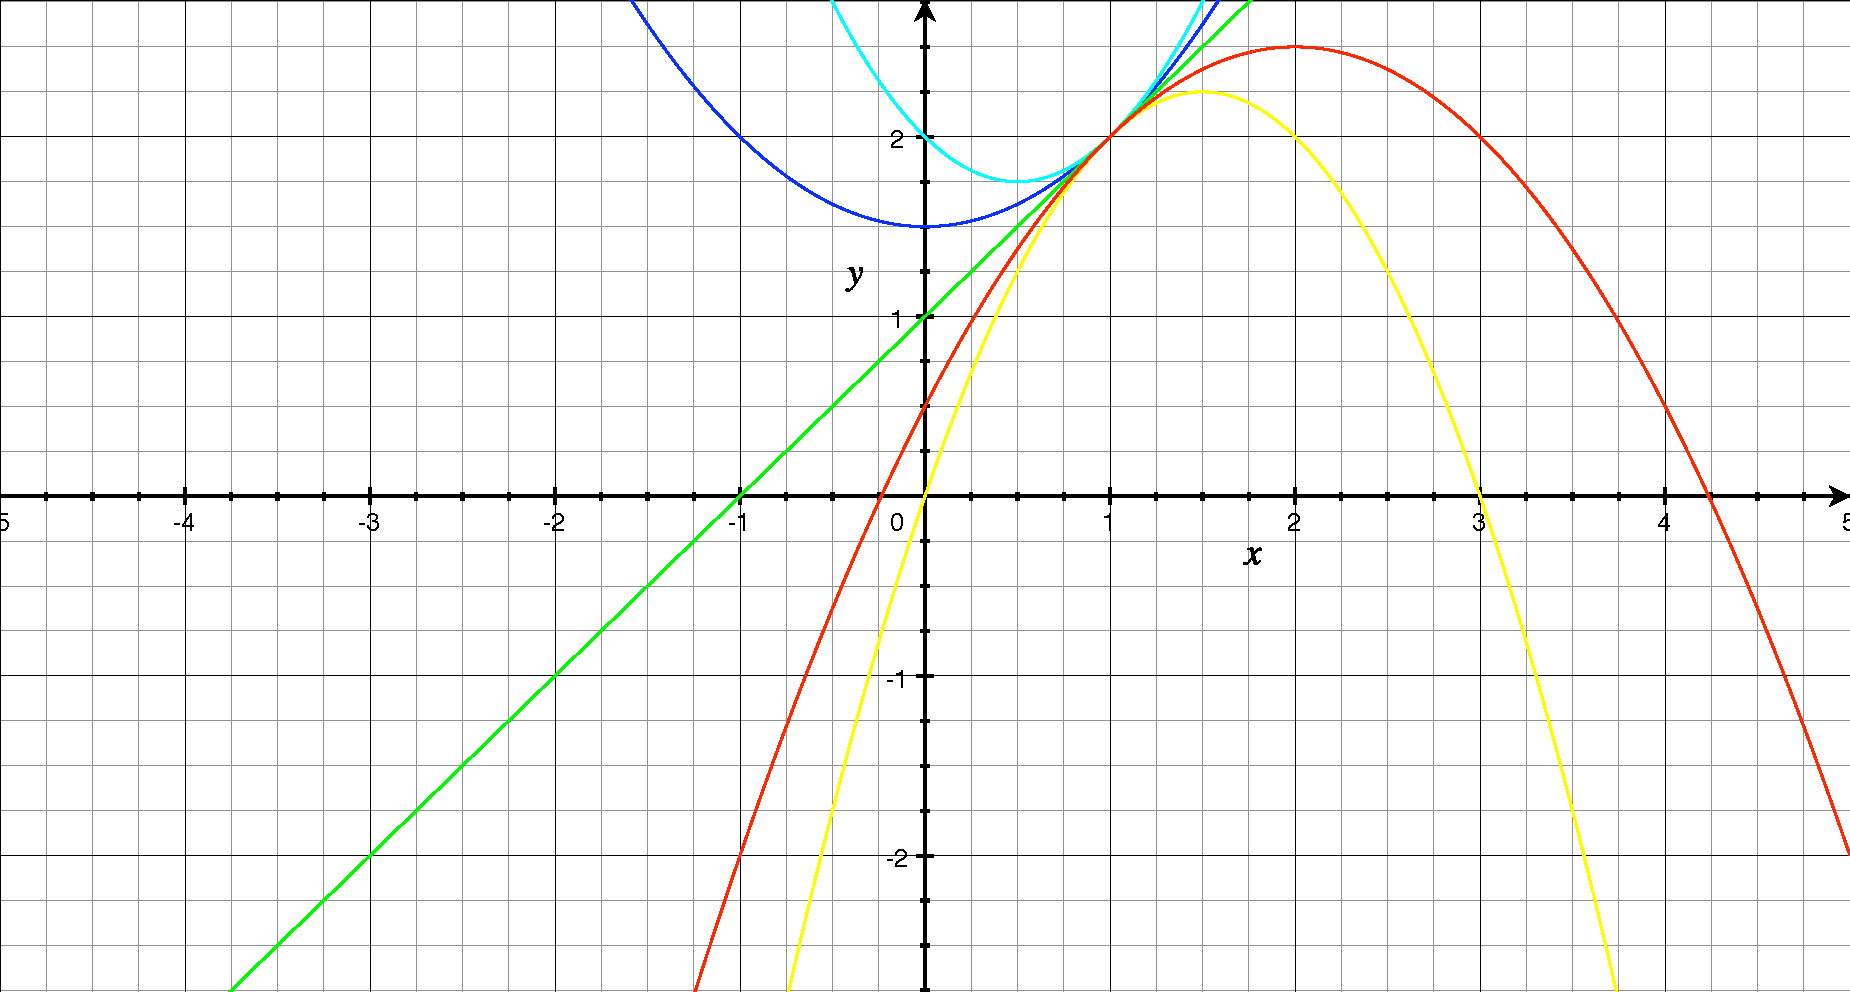
\includegraphics[width=12cm]{der_seconde}
% % ($f''(a) \in \{+2$ pour la fonction bleu clair, $f''(a)=+1$ pour la fonction bleu foncé, $f''(a)=0$ pour la fonction verte, $f''(a)=-1$ pour la fonction rouge et $f''(a)=-2$ pour la fonction jaune)}
% \end{frame}
%\end{frame}

\subsection{Asymptotes}
\begin{frame}
  \begin{definition}
    Une asymptote est une droite (ou une courbe) de laquelle le graphe d'une fonction donnée se rapproche.
  \end{definition}
  On distingue généralement les asymptotes
  \begin{itemize}
  \item \og verticales\fg{},
  \item \og horizontales\fg{} et
  \item \og obliques\fg{}.
  \end{itemize}
  
  Dans la suite nous considérons une fonction réelle $f$.
\end{frame}

\begin{frame}
  \begin{definition}
    La droite d'équation $x=a$ est une \Defn{asymptote verticale} au graphe de $f$ si
    \begin{equation*}
      \lim_{x \to a^-} f(x) = \pm \infty \quad \textrm{ ou } \quad \lim_{x \to a^+} f(x) = \pm \infty
    \end{equation*}
  \end{definition}
  \begin{example}
    La droite \(x = 0\) est asymptote verticale au graphe de \(x \mapsto \frac{1}{x}\).\pause

    La droite \(x = \frac{\pi}{2}\) est asymptote verticale au graphe de la fonction tangente.
  \end{example}
\end{frame}

\begin{frame}
  \begin{definition}
    La droite d'équation $y=b$ est une \Defn{asymptote horizontale} au graphe de $f$ lorsque
    \begin{equation*}
      \lim_{x \to - \infty} f(x) = b \quad \mbox{ ou } \quad \lim_{x \to +\infty} f(x) = b
    \end{equation*}
  \end{definition}
  \begin{example}
    La droite d'équation \(y = 0\) est asymptote horizontale (tant en \(+\infty\) qu'en \(-\infty\)) au graphe de \(x \mapsto \frac{1}{x}\)\pause

    La droite d'équation \(y = \pi/2\) est asymptote horizontale (en \(+\infty\)) au graphe de \(\arctan\).\pause

    La droite d'équation \(y = -\pi/2\) est asymptote horizontale (en \(-\infty\)) au graphe de \(\arctan\).
  \end{example}
\end{frame}
\begin{frame}
  \begin{example}
    \includegraphics[width=12cm]{arctan}
  \end{example}
\end{frame}

\begin{frame}
  \begin{definition}
La droite d'équation $y=mx+b$ où $m \neq 0$ est une \Defn{asymptote oblique} au graphe de $f$  si
\begin{equation*}
\lim_{x \to - \infty} \left[ f(x)-(mx+b)\right] =0 \quad \mbox{ ou } \quad
\lim_{x \to + \infty} \left[ f(x) -(mx+b)\right] = 0
\end{equation*}\pause
C'est le fait que $m \neq 0$ qui justifie l'adjectif \og oblique\fg{}.\pause{} Lorsque \(m = 0\), on retrouve le cas d'une asymptote horizontale.
\end{definition}
\end{frame}
\begin{frame}
\begin{example}
  La droite d'équation \(y = x + 1\) est asymptote oblique au graphe de la fonction \(f\) définie par
  \begin{equation*}
    f(x) = \frac{x^{2}}{x-1}
  \end{equation*}
  \begin{center}
    \includegraphics[height=5cm]{xpow2overxminus1}
  \end{center}
\end{example}
\end{frame}

\begin{frame}
  La proposition suivante permet de calculer \(m\) et \(b\) lorsqu'ils existent.
  \begin{proposition}
    La droite $y=mx+b$, où $m \neq 0$, est asymptote oblique au graphe de $f$ pour $x$ tendant vers $+\infty$ si et seulement si
    \begin{equation*}
      \lim_{x \to + \infty} \frac{f(x)}{x} = m \neq 0 \quad \mbox{ et } \quad
      \lim_{x \to + \infty} \left[ f(x)-mx \right] = b
    \end{equation*}
  \end{proposition}
\end{frame}

\begin{frame}
  \begin{example}
    Le cas de la fonction \(\ln\) est intriguant car
    \begin{equation*}
      \limite x \infty \frac{\ln x}{x} = 0
    \end{equation*}
    (en application de la règle de l'Hospital), mais
    \begin{equation*}
      \limite x \infty \ln x = +\infty
    \end{equation*}
    dès lors il n'y a en réalité pas d'asymptote horizontale, ni oblique !\pause{}
    (Par contre il y a bien une asymptote verticale \(x = 0\).)
  \end{example}
\end{frame}

\section{Approximation de Taylor}
\subsection{Ordre 1}% FIXME: intégrer au syllabus -- dans le syllabus mettre taylor tout ensemble ?
\begin{frame}
  \begin{definition}
    \(f\) est dérivable en \(a\) (intérieur à son domaine) si la limite suivante existe :
    \begin{equation*}
      \limite x a \frac{f(x) - f(a)}{x-a}.
    \end{equation*}
  \end{definition}\pause
  En d'autres termes, il existe un réel, noté \(f'(a)\), tel que
  \begin{equation*}
    \limite x a \frac{f(x) - f(a)}{x-a} - f'(a) = 0
  \end{equation*}\pause{}
  ou encore
  \begin{equation*}
    \limite x a \frac{f(x) - (f(a) + f'(a) (x-a))}{x-a} = 0
  \end{equation*}\pause{}
  ou encore, en notant \(T(x) = f(a) + f'(a)(x-a)\), cela revient à dire que
  \begin{center}
    \(f(x) - T(x)\) est un \(o({x-a})\) pour \(x \to a\).
  \end{center}
  \begin{remark}
     \(T\) est une fonction polynômiale de degré \(1\) dont le graphe est simplement la tangente au graphe de \(f\) au point \((a,f(a))\).
  \end{remark}
\end{frame}

\begin{frame}{Questions de notations}% FIXME: intégrer au syllabus et déplacer ceci avec d'autres questions de notation ?
  On peut écrire~:\pause
  \begin{align*}
    \uncover<+->{f(x) = f(a) + f'(a) (x-a) + o(x-a)\\}
    \uncover<+->{    \intertext{ou encore}
    f(a + \delta x) = f(a) + f'(a) \delta x + o(\delta x)}
    \uncover<+->{    \intertext{ou encore}
    f(x + \delta x) = f(x) + f'(x) \delta x + o(\delta x)}
  \end{align*}
\end{frame}

\begin{frame}
  \begin{remark}
  Si $f$ est dérivable au point $a$, la droite d'équation
  \begin{equation*}
    \boxed{y=f'(a)(x-a)+f(a)}
  \end{equation*}
  est la \Defn[tangente]{droite tangente au graphe de $f$ au point $(a,f(a))$} ou \Defn[droite!tangente]{droite tangente de $f$ en $a$}.
\end{remark}
\end{frame}

\begin{frame}
  \begin{remark*}
    \begin{itemize}
    \item Idée générale : si \(f\) est une fonction quelconque, on aimerait l'approximer, le mieux possible, par des fonctions plus simples.\pause{}

    \item Il n'est pas forcément possible de bien approximer \emph{partout},\pause{} donc on se contentera ici de bien approximer près d'un point \(a\) fixé dans le domaine.
    \end{itemize}
  \end{remark*}\pause{}
  
  Le polynôme \(T\) défini ci-dessus est une bonne approximation de \(f\) près de \(x = a\).\pause{} Si on note \(R(x) = f(x) - T(x)\),\pause{} on a vu que \(R(x)\) tend vers \(0\) plus vite que \((x-a)\) pour \(x \to a\).\pause{}
  \begin{definition}
    \(T\) défini par \(T(x) = f(a) + f'(a)(x-a)\) est le \emph{polynôme de Taylor d'ordre \(1\)} de la fonction \(f\) au point \(a\).
  \end{definition}
\end{frame}

\begin{frame}
  \begin{itemize}
  \item Si on essaye d'approximer par des polynômes de degré plus élevé, a-t-on une meilleure approximation ?\pause{} Oui ! \pause{}
  \item Peut-on approximer une fonction par autre chose que des polynômes ? \pause{} Oui !\pause{} (mais on ne le verra pas ici.)
  \end{itemize}
\end{frame}

\subsection{Ordres supérieurs}
\begin{frame}% ceci n'accrochait pas les étudiants -- voir les slides du cours suivant.
\begin{definition}
Le polynôme \(T_{f,a,n}\) défini par\pause{}
\begin{align*}
T_{f,a,n}(x) &=\sum_{k=0}^n f^{\underline{k}}(a) \frac{(x-a)^k}{k!}\\
&=f(a) + f'(a)(x-a) + f''(a) \frac{(x-a)^2}{2} + \cdots + f^{\underline{n}}(a) \frac{(x-a)^n}{n!}
\end{align*}
est le \Defn{polynôme de Taylor} d'ordre $n$ de $f$ au point $a$.\pause{} Ici $f^{\underline{k}}$ désigne la dérivée $k$-ème de~$f$.
\end{definition}\pause{}

\begin{remark*}% ceci n'accrochait pas les étudiants
Le polynôme de Taylor d'ordre $n$ de $f$ est un polynôme de degré (au plus) $n$ dont la dérivée d'ordre $k$ au point $a$ est égale à la dérivée d'ordre \(k\) de $f$ au point $a$, pour $k = 0, \ldots, n$.\pause{} C'est le seul tel polynôme.
\end{remark*}
\end{frame}
\begin{frame}
  \begin{definition}
    L'erreur commise en approximant $f(x)$ par son polynôme de Taylor \(T_{f,a,n}\) d'ordre $n$ est notée $R_n(x)$, et s'appelle le \Defn{reste} d'ordre $n$ de $f$. Donc~:
    \begin{equation*}
      R_n(x) = f(x)-T_{f,a,n}(x)
    \end{equation*}
  \end{definition}

  \begin{remark*}
    Notons que le reste possède un signe~: si $R_n(x) > 0$ alors $T_{f,a,n}(x) < f(x)$ (sous-approximation), et si $R_n(x) < 0$ alors $T_{f,a,n}(x) > f(x)$ (sur-approximation).
  \end{remark*}
\end{frame}
\course{12} % Taylor d'ordre supérieur
\begin{frame}{Informations}
  \pause
  \begin{itemize}
  \item Afin de concentrer votre effort, une liste de définition et résultats théoriques à connaître a été mise en place sur mon site web.\pause{}
  \item En particulier, il faut noter que la matière pour la partie théorique ne concernera que les dix premiers cours (attention : c'est moins qu'initialement annoncé !).
  \end{itemize}
\end{frame}
\section{Approximation de Taylor}
\subsection{Polynômes de Taylor d'ordre supérieur}
\begin{frame}
  \begin{rappel}
    Si \(f\) est dérivable en \(a\), alors \(T\) défini par \(T(x) = f(a) + f'(a) (x-a)\) est une \og bonne approximation de \(f\) près de \(a\)\fg{}.\pause{} On l'appelle le \og polynôme de Taylor d'ordre \(1\) de \(f\) en \(a\)\fg{}.
  \end{rappel}\pause

  Plus précisément~:\pause
  \begin{equation*}
    \limite{x}{a} \frac{f(x)-T(x)}{x-a} = 0\pause \text{ ou encore } f(x) = T(x) + o(\abs{x-a})
  \end{equation*}\pause

  \begin{block}{Paraphrase}\pause
    \(f(x)-T(x)\) tend vers \(0\) plus vite que \(x-a\).
  \end{block}
\end{frame}
\begin{frame}
  \begin{block}{But}\pause{}
    Nous voulons de meilleures approximations, du type :\pause{}
    \begin{center}
      \og \(f(x) - \text{\textbf{???}}\) tend vers \(0\) plus vite que \((x-a)^{2}\)
    \end{center}\pause{}
    Que mettre ? \pause{} Réponse : le polynôme de taylor d'ordre \(2\) !
  \end{block}
\end{frame}
\begin{frame}
  \begin{definition}
    Le polynôme de Taylor d'ordre \(2\) de \(f\) en \(a\) est \(T_{f,a,2}\)\pause{}
    \begin{equation*}
      T_{f,a,2}(x) = f(a) + f'(a) (x-a) + f"(a) \frac{(x-a)^{2}}{2}
    \end{equation*}
  \end{definition}
  \begin{remark*}\pause
    \begin{align*}
      \uncover<+->{T_{f,a,2}'(x) &= f'(a) + f"(a) (x-a) \Rightarrow T_{f,a,2}'(a) = f'(a)\\}
      \uncover<+->{T_{f,a,2}"(x) &= f"(a) \Rightarrow T_{f,a,2}"(a) = f"(a)}
    \end{align*}
  \end{remark*}
\end{frame}

\begin{frame}
  \begin{definition}
    Le polynôme de Taylor d'ordre \(3\) de \(f\) en \(a\) est \(T_{f,a,3}\)\pause{}
    \begin{equation*}
      T_{f,a,3}(x) = f(a) + f'(a) (x-a) + f"(a) \frac{(x-a)^{2}}{2!} + f'''(a) \frac{(x-a)^{3}}{3!}
    \end{equation*}
  \end{definition}
  \begin{remark*}\pause{}
    \begin{align*}
      \uncover<+->{T_{f,a,3}'(x) &= f'(a) + f"(a) (x-a) + f'''(a) \frac{(x-a)^{2}}{2!} \Rightarrow T_{f,a,2}'(a) = f'(a)\\}
      \uncover<+->{T_{f,a,3}"(x) &= f"(a) + f'''(a) (x-a) \Rightarrow T_{f,a,3}"(a) = f"(a)\\}
      \uncover<+->{T_{f,a,3}'''(x) &= f'''(a) \Rightarrow T_{f,a,3}'''(a) = f'''(a)}
    \end{align*}
  \end{remark*}
\end{frame}
\begin{frame}
    \begin{definition}
    Le polynôme de Taylor d'ordre \(n\) de \(f\) en \(a\) est \(T_{f,a,n}\)\pause{}
    \begin{align*}
      T_{f,a,n}(x) &=\sum_{k=0}^n f^{\underline{k}}(a) \frac{(x-a)^k}{k!}\\[-.5\baselineskip]
                   &=f(a) + f'(a)(x-a) + f''(a) \frac{(x-a)^2}{2} + \cdots + f^{\underline{n}}(a) \frac{(x-a)^n}{n!}
    \end{align*}
    où $f^{\underline{k}}$ désigne la dérivée $k$-ème de~$f$.
  \end{definition}\pause{}
  \begin{remark*}
    Les dérivées de $f$ et de $T_{f,a,n}$ en $a$ co\"\i{}ncident jusqu'à l'ordre $n$.\pause{}

    Si on note \(R_{f,a,n} = f - T_{f,a,n}\), on a 
    \begin{equation*}
      R_{f,a,n}(a) = R'_n(a) = \ldots = R_{f,a,n}^{\underline{n}}(a)=0
    \end{equation*}\pause{}
    Cette fonction est donc \og très plate\fg{} autour de $a$.
  \end{remark*}
\end{frame}

\begin{frame}[<+->]
  Écrivons le polynôme de Taylor de $f(x) = \sin x$ autour de $a = 0$.\pause{}
  \begin{equation*}
    f'(x) = \cos x \qquad f''(x) = - \sin x \qquad f'''(x) = - \cos x \qquad f''''(x) = \sin x
  \end{equation*}
  Dès lors :
  \begin{equation*}
    f(0) = 0 \qquad f'(0) = 1 \qquad f''(0) = 0 \qquad f'''(0) = -1 \qquad 
    f''''(0) = 0
  \end{equation*}
  Et donc nous avons :
  \begin{align*}
    \uncover{T_{f,0,0}(x) & = 0\\}
    \uncover{T_{f,0,1}(x) & = 0 + 1 \cdot x = x\\}
    \uncover{T_{f,0,2}(x) & = 0 + 1 \cdot x + 0 = x\\}
    \uncover{T_{f,0,3}(x) & = 0 + 1 \cdot x + 0 + (-1) \cdot \frac{x^3}{3!} = x - \frac{x^{3}}{3!}\\}
    \uncover{T_{f,0,4}(x) & = 0 + 1 \cdot x + 0 + (-1) \cdot \frac{x^3}{3!} + 0 = x - \frac{x^{3}}{3!}\\}
    \uncover{T_{f,0,5}(x) & = x - \frac{x^{3}}{3!} + \frac{x^5}{5!}}
  \end{align*}
\end{frame}

\begin{frame}
  \begin{center}
    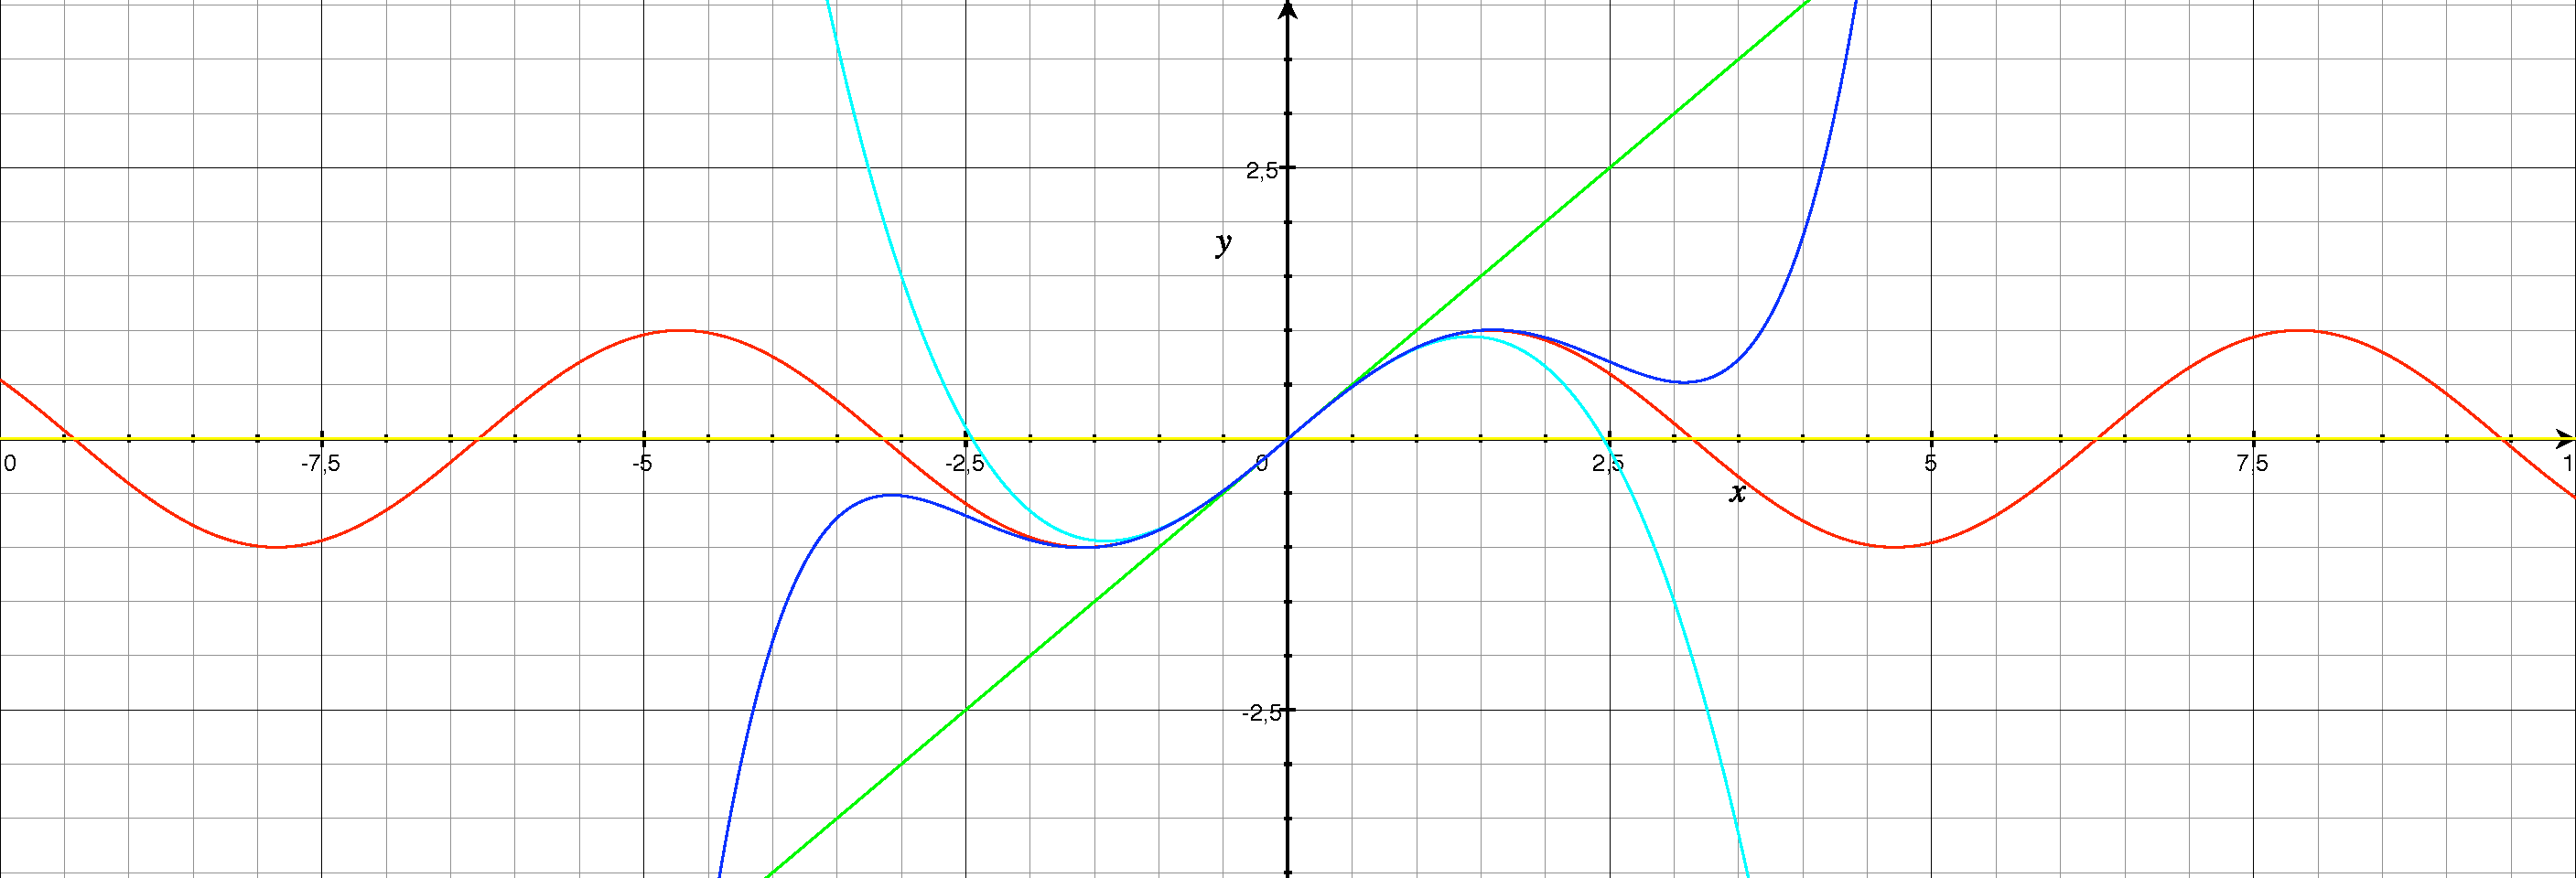
\includegraphics[width=12cm,clip,trim=350 0 350 0]{Taylor_sin.pdf}
  \end{center}
\end{frame}

\begin{frame}
  Voyons maintenant à quoi ressemble la fonction de reste $R_{f,a,n} = f - T_{f,a,n}$~:
  \begin{center}
    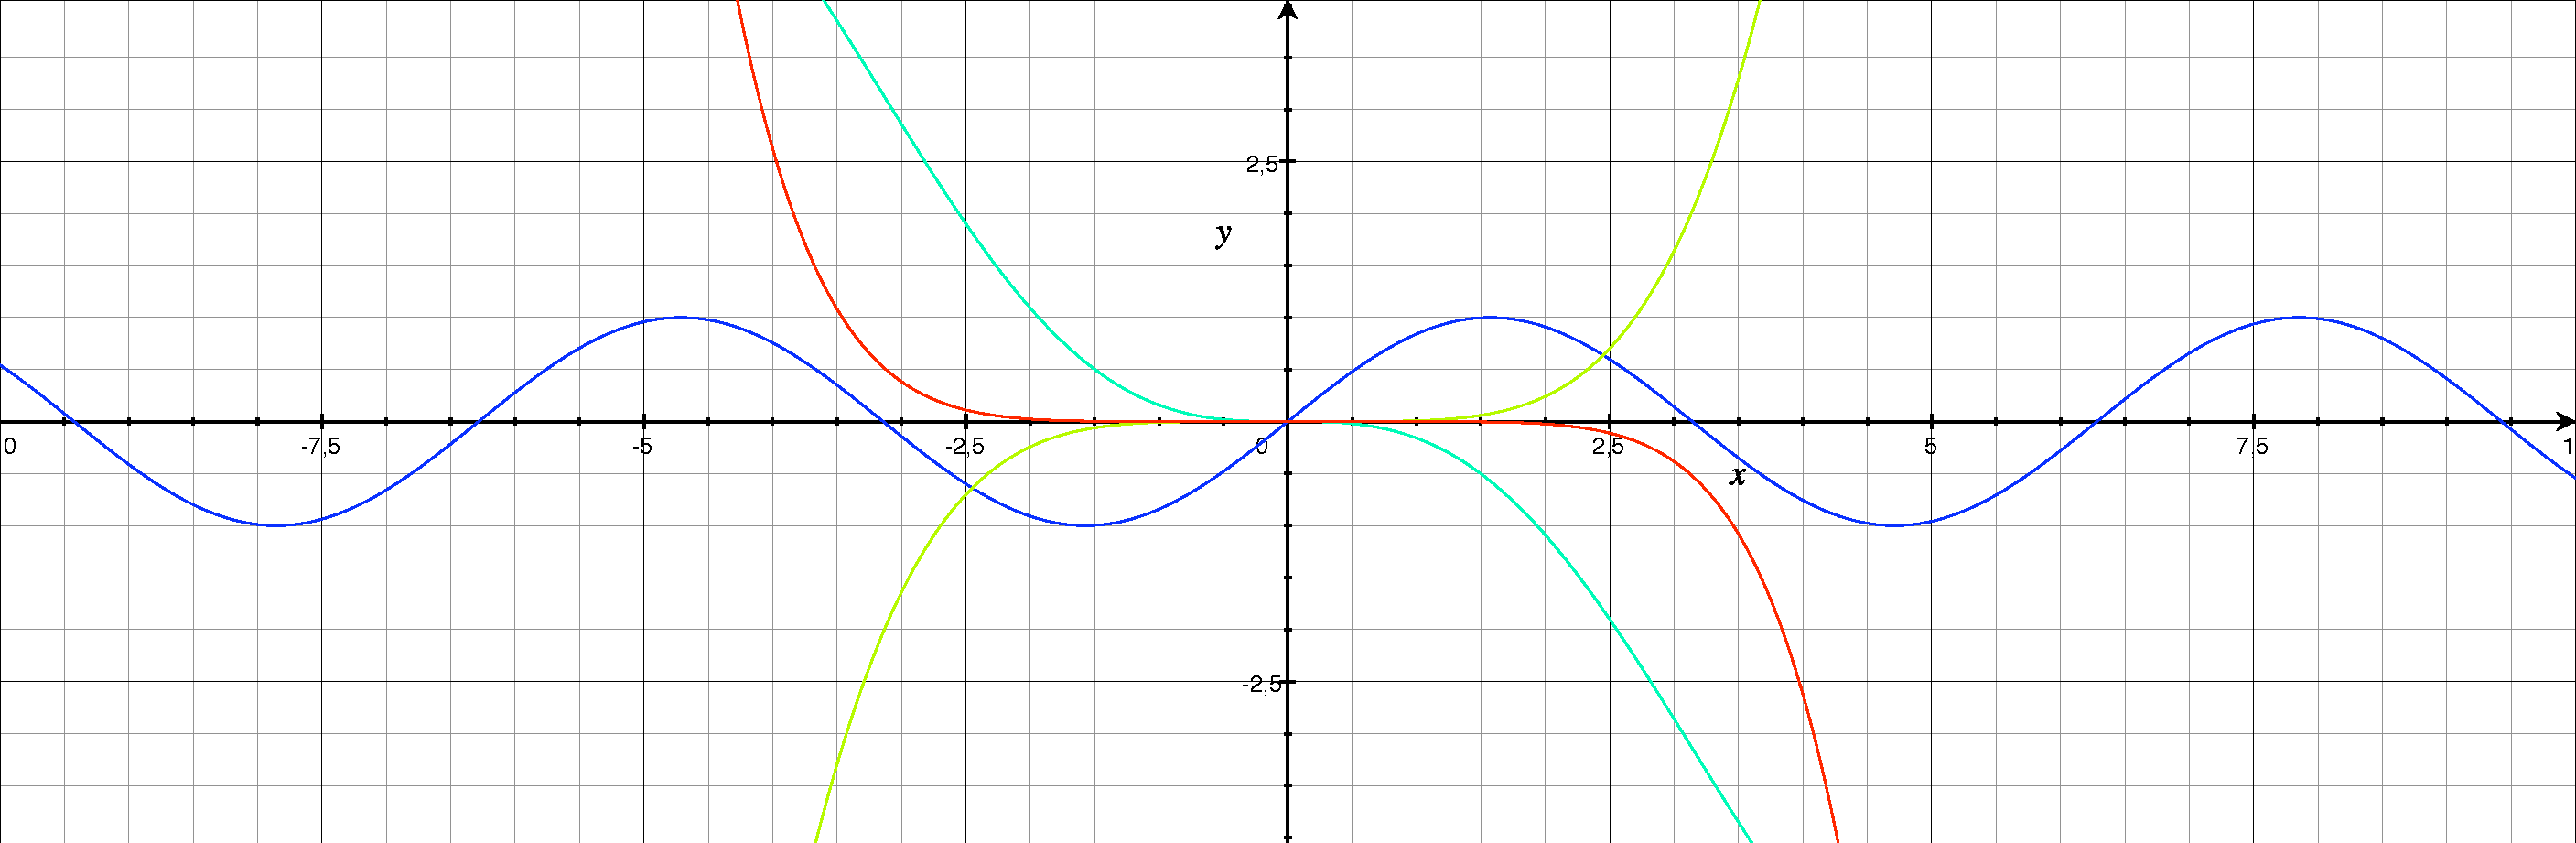
\includegraphics[width=15cm]{Taylor_sin_reste.pdf}
  \end{center}
\end{frame}

\begin{frame}
  \begin{example}
    Prenons maintenant $f(x) = \ln x$ et $a = 1$.\pause{}
    \begin{equation*}
      \uncover<+->{f'(x) = x^{-1}}
      \uncover<+->{\qquad f''(x) = - x^{-2}} 
      \uncover<+->{\qquad f'''(x) = 2 x^{-3}} 
      \uncover<+->{\qquad f''''(x) = -6 x^{-4}}
    \end{equation*}\pause{}
    On devine une formule générale pour $f^{\underline{k}}(x)$, valable pour $k \geqslant 1$~:\pause
    \begin{equation*}
      f^{\underline{k}}(x) = (-1)^{k-1}(k-1)! \, x^{-k}
    \end{equation*}\pause
    Évaluons maintenant les dérivées de $f$ en $a = 1$~:\pause
    \begin{equation*}
      \uncover<+->{f(1) = 0}
      \uncover<+->{\qquad f'(1) = 1}
      \uncover<+->{\qquad f''(1) = -1}
      \uncover<+->{\qquad f'''(1) = 2}
      \uncover<+->{\qquad f'''''(1) = -6}
    \end{equation*}\pause
    Les polynômes de Taylor de $f(x) = \ln x$ en $a = 1$ sont donc~:
    \begin{align*}
      \uncover<+->{T_0(x) &= 0 \quad }
      \uncover<+->{T_1(x) = 0 + 1 \cdot (x-1)\\}
      \uncover<+->{T_2(x) &= 0 + 1 \cdot (x-1) - 1 \frac{(x-1)^2}{2}\\}
      \uncover<+->{T_3(x) &= 0 + 1 \cdot (x-1) - 1 \frac{(x-1)^2}{2} + 2 \frac{(x-1)^3}{6}}
    \end{align*}\pause{}
    \begin{equation*}
      T_{f,a,n}(x) = (x-1) - \frac{1}{2} (x-1)^2 + \frac{1}{3} (x-1)^3 
      + \cdots \pm \frac{1}{n} (x-1)^n
    \end{equation*}
  \end{example}
\end{frame}
\begin{frame}
    \begin{center}
      \includegraphics[width=8cm]{Taylor_ln.pdf}%FIXME: colors are wrong, legend is misplaced.
    \end{center}
\end{frame}

\subsection*{Théorème de Taylor et formule du reste}
\begin{frame}% FIXME: intégrer au syllabus
  Le théorème suivant exprime que le polynôme de Taylor est la meilleure approximation polynomiale de \(f\) près de \(a\) :
  \begin{theorem}\label{thmtaylor}\pause{}
    Le polynôme de Taylor \(T_{f,a,n}\) est l'unique polynôme de degré inférieur à \(n\) pour lequel la fonction de reste, \(R_{f,a,n}\), est un \og petit o\fg{} de \((x-a)^{n}\) quand \(x \to a\).
  \end{theorem}\pause{}
  C'est la meilleure, mais est-elle bonne ?
\end{frame}
% \begin{frame}
%   Prenons \(x\) proche de \(a\), disons \(x > a\). Comment évaluer \(R_{f,a,n}(x)\) ?\pause{}
  
%   % Nous savons qu'il existe \(c\in \interoo{a,x}\) tel que
%   % \begin{equation*}
%   %   f'(c) = \frac{f(x) - f(a)}{x-a}
%   % \end{equation*}
%   % c'est-à-dire
%   % \begin{equation*}
%   %   f(x) = f(a) + f'(c) (x-a)
%   % \end{equation*}
%   % ou encore
%   % \begin{equation*}
%   %   R_{f,a,0} = f'(c) (x-a).
%   % \end{equation*}
% \end{frame}

\begin{frame}
  Prenons \(x\) proche de \(a\), disons \(x > a\). Comment évaluer \(R_{f,a,n}(x)\) ?\pause{}
  
\begin{theorem}[Formule du reste de Lagrange]
  Si $f$ est dérivable $(n+1)$-fois dans un intervalle $I=\interoo{a-\delta,a+ \delta}$\pause{}, alors pour chaque $x \in I$~:\pause{}
\begin{equation*}
    R_{f,a,n}(x) = f^{\underline{n+1}}(t) \frac{(x-a)^{n+1}}{(n+1)!}
  \end{equation*}
    pour un $t$ entre $a$ et $x$ (\(t\) dépend donc de \(x\) !)\pause{}, c'est-à-dire\pause{}
\begin{equation*}
    f(x) =
    f(a)+f'(a)(x-a)+\cdots+f^{\underline{n}}(a) \frac{(x-a)^n}{n!}+ f^{\underline{n+1}}(t) \frac{(x-a)^{n+1}}{(n+1)!}
  \end{equation*}
    pour un $t$ entre $a$ et $x$.
\end{theorem}
\end{frame}

% Voyons ce signifie ce théorème dans le cas le plus simple, quand $n = 0$~:
% \begin{equation*}
% f(x) = f(a) + f'(t)(x-a) 
% \end{equation*}
% pour un $t$ entre $a$ et $x$. Si on prend $x > a$ cela signifie qu'il \emph{existe} $t \in \interoo{a,x}$ tel que
% \begin{equation*}
% f'(t) = \frac{f(x)-f(a)}{x-a}
% \end{equation*}
% ce n'est rien d'autre que le théorème des accroissements finis~!

\begin{frame}{Exemple d'utilisation du théorème}
  Pour $f(x) = \ln x$ et $a = 1$.\pause{}
  \begin{equation*}
    \ln 2 = 1 - \frac{1}{2} + \frac{1}{3} - \cdots + (-1)^{n-1} \frac{1}{n} + R_{f,a,n}(2)
  \end{equation*}\pause{}
  où
  \begin{equation*}
    R_{f,a,n}(2) = \frac{(-1)^{n}}{n+1} t^{-n-1}
  \end{equation*}
  pour un $t$ entre $a = 1$ et $x = 2$.\pause{}

\begin{remark*}
  $t$ est positif et donc le \emph{signe} de l'erreur est $(-1)^n$.\pause{}
  \begin{itemize}
  \item \(n\) est pair \(\Longrightarrow\) sous-approximation ;\pause{}
  \item \(n\) est impair \(\Longrightarrow\) sur-approximation.
  \end{itemize}
\end{remark*}\pause{}

La quantité \(\abs{R_{f,a,n}(2)}\) décroit avec \(t\)\pause{}, donc au pire \(t = 1\)\pause{} et l'erreur absolue vaut alors \(\frac{1}{n+1}\).\pause{} On peut donc écrire :
\begin{equation*}
  \abs{R_{f,a,n}(2)} < \frac{1}{n+1}.
\end{equation*}
\end{frame}
\begin{frame}{Comment choisir $n$, le nombre de termes dans notre approximation, pour être sûr de calculer \emph{une} décimale correcte de $\ln 2$~?}
  \pause{}
Remarquons d'abord que si \(n \geqslant 9\), alors
\begin{equation*}
  |R_{f,a,n}(2)| < 10^{-1}.
\end{equation*}\pause{}
Calculons $T_9(2)$~:\pause{}
\begin{equation*}
T_9(2) = 1 - \frac{1}{2} + \frac{1}{3} - \frac{1}{4} 
+ \frac{1}{5} - \frac{1}{6} + \frac{1}{7} - \frac{1}{8} + \frac{1}{9} = 0,745634920\ldots
\end{equation*}\pause{}
qui est une sur-approximation\pause{}, puis $T_{10}(2)$~:\pause{}
\begin{equation*}
T_{10}(2) = 1 - \frac{1}{2} + \frac{1}{3} - \frac{1}{4} 
+ \frac{1}{5} - \frac{1}{6} + \frac{1}{7} - \frac{1}{8} + \frac{1}{9}
- \frac{1}{10} = 0,645634920\ldots
\end{equation*}
qui est une sous-approximation.\pause{} Ces deux nombres sont à une distance moins de $10^{-1}$ de $\ln 2$.\pause{} Mais quel est celui dont la première décimale est correcte~?\pause{} Il faut plus de termes\pause{}, en fait plus de 70 ({!})\pause{}, pour conclure que $\ln 2 = 0,6\ldots$
%% elisp snippet to check 

% (defun yf/approx-ln-by-taylor-exp (n)
%   (let ((res 0))
%     (loop for i from 1 to n do
%          (setq res (+ res (* (if (oddp i) 1 -1) (/ 1 (float i))))))
%     res))
% (mapconcat #'prin1-to-string
%  (loop for i from 69 to 75 by 2
%        collect (list i (yf/approx-ln-by-taylor-exp i))) "\n")
\end{frame}

\begin{frame}
  \begin{example}
    Dans le cas de \(f(x) = \sin(x)\) et \(a = 0\)\pause{}, on peut calculer \(f(1)\) avec une bonne précision très rapidement.\pause{} Le reste s'écrit
    \begin{equation*}
      R_{f,a,n}(x) = f^{\underline{n+1}}(t) \frac{(1-0)^{n+1}}{(n+1)!}
    \end{equation*}\pause{}
    mais cette fois \(f^{\underline{n+1}}(t)\) est toujours inférieur à \(1\) en valeur absolue (car les dérivées successives de \(\sin\) sont \(\cos\), \(-\sin\), \(-\cos\), \(\sin\), etc.).\pause{} On en déduit
    \begin{equation*}
      \abs{R_{f,a,n}(x)} \leq \frac{1}{(n+1)!}
    \end{equation*}\pause{}
    ce qui diminue très rapidement : \(\frac{1}{2}, \frac{1}{6}, \frac{1}{24}, \frac{1}{120}, \frac{1}{720}, \frac{1}{5040}\),\pause{} il suffit donc de quelques termes pour obtenir une précision de plusieurs décimales.
  \end{example}
\end{frame}

\begin{frame}{Que retenir~?}
  \begin{itemize}[<+->]
  \item L'approximation de Taylor est la meilleure, mais pas toujours très bonne.
  \item Il faut contrôler le terme d'erreur !
  \end{itemize}\pause{}

  \begin{block}{Comment choisir \(a\) ?}\pause{}% FIXME: intégrer au syllabus
    Il faut choisir le point \(a\) pour que les calculs soient faisables.
  \end{block}
\end{frame}

\begin{frame}{Remarques pour le test}
  Pour le test de "novembre" du 29 octobre, il y a deux auditoires prévus. Les étudiants concernés (tous sauf PHAR1) se répartissent comme suit :
  \begin{itemize}
  \item BIOL1 : Auditoire Chavanne (Bâtiment U, porte D)% avant j'avais mis les GEOG1 avec.
  \item Autres : Auditoire Janson.
  \end{itemize}\pause

  Munissez-vous de :
  \begin{itemize}\pause
  \item votre carte d'étudiant,\pause
  \item papier (max 4 feuilles, vierges de toute annotation)\pause
  \item stylo-bille ou crayon de couleur foncée
  \end{itemize}
\end{frame}
\begin{frame}
  Tout autre accessoire non strictement nécessaire est \textbf{interdit}. En particulier (liste non-exhaustive):
  \begin{itemize}
  \item GSM, ordinateur, calculatrice : sont interdits !\pause
  \item Notes de cours et syllabus : sont interdits !
  \end{itemize}
\end{frame}
\begin{frame}
  La matière est :\pause
  \begin{description}
  \item[Exercices] Séances 1 à 10
  \item[Théorie] Cours  1 à 10 
  \end{description}\pause

  \begin{remark}
    Le test est important pour vous situer par rapport aux exigences du cours.\pause

    Si vous réussissez mieux en janvier qu'en octobre, la note d'octobre est oubliée.\pause Sinon elle compte pour le quart de votre note de janvier.
  \end{remark}
\end{frame}
\course{13}% Primitives: début
\begin{frame}
\tableofcontents
\end{frame}
\section{Primitives}
\subsection{Motivation}
\subsubsection{Vitesse et position}
\begin{frame}\pause{}% FIXME: intégrer au syllabus
  Considérons une droite munie d'un repère cartésien, c'est-à-dire une droite graduée.\pause{}

  Soit \(f : \RR \to \RR : t \mapsto f(t)\) une fonction dont la valeur \(f(t\)) représente la coordonnée d'un mobile à l'instant \(t\) le long de cette droite.

  \begin{example}\pause{}
    Si on note \(f(t)\) la hauteur d'un yoyo au cours du temps, on pourrait modéliser ceci par \(f(t) = cos(t)\).\pause{}
    \begin{itemize}[<+->]
    \item À l'instant \(t = 0\), le mobile est à hauteur \(1\),
    \item puis descend pour arriver à hauteur \(-1\),
    \item remonte ensuite pour retourner à hauteur \(1\),
    \item et ainsi de suite\dots{}
    \end{itemize}
  \end{example}\pause{}

  Dans cette situation, la quantité
  \begin{equation*}
    \frac{f(b)-f(a)}{b-a}
  \end{equation*}
  représente\pause{} la distance parcourue\pause{} rapportée au temps passé à la parcourir\pause{} : c'est la \emph{vitesse moyenne} du mobile entre les instants \(a\) et \(b\).
\end{frame}
\begin{frame}% FIXME: intégrer au syllabus dans la partie "dérivées"
  \begin{remark}
    Notons que le signe de la vitesse moyenne indique le sens du déplacement !
  \end{remark}\pause{}

  Lorsque \(a\) et \(b\) sont de plus en proches, la vitesse moyenne tend vers la quantité
  \begin{equation*}
    \limite{b}{a}  \frac{f(b)-f(a)}{b-a} = f'(a).
  \end{equation*}\pause{}
  C'est la \emph{vitesse instantannée} du mobile à l'instant \(a\).\pause{}

  \begin{center}
    \fbox{\parbox{0.9\linewidth}{La vitesse instantannée est la dérivée de la position par rapport au temps.}}
  \end{center}\pause

  \begin{remark*}
    Connaissant la vitesse instantannée en chaque instant, comment retrouver la position ?\pause{} Notons qu'il faut au minimum connaître la position initiale !
  \end{remark*}
\end{frame}

\subsubsection{Équation aux dérivées pour une population}
\begin{frame}% FIXME: intégrer au syllabus
  \begin{question}
    On considère une population de bactéries au cours du temps, et on note \(p(t)\) le nombre de bactéries à l'instant \(t\).\pause{} On suppose que le taux de croissance de ces bactéries est lié à deux facteurs : le nombre de bactéries, et les ressources disponibles. On peut modéliser cela par l'équation
    \begin{equation*}
      p'(t) = p(t)(K - p(t))
    \end{equation*}
    où \(K\) représente les ressources disponibles.\pause{}

    Quelles sont les fonctions qui vérifient cette équation en tout \(t\) ?\pause{}
  \end{question}
  \begin{remark}
    Une telle équation est une \emph{équation différentielle}.
  \end{remark}
\end{frame}
\begin{frame}% FIXME: intégrer au syllabus
  \begin{answer}
    Supposons que la population ne disparait pas (\(p(t)\neq 0\)) et ne dépasse jamais les ressources (\(p(t)\neq K\)), alors~:\pause{}
    \begin{equation*}
      \frac{p'(t)}{p(t)(K-p(t))} = 1
    \end{equation*}\pause{}
    Notons \(f(x) = \frac{1}{x(K-x)}\). Alors l'équation se ré-écrit~:\pause{}
    \begin{equation*}
      f(p(t)) p'(t) = 1
    \end{equation*}\pause{}
    C'est-à-dire, en notant \(F\) une fonction telle que \(F' = f\), on aurait
    \begin{equation*}
      (F(p(t)))' = 1.
    \end{equation*}\pause{}
    Si on savait trouver des fonctions dont la dérivée est une fonction donnée, on pourrait terminer ces calculs !
  \end{answer}
\end{frame}

\subsubsection{Équation aux dérivées pour le ressort}

\begin{frame}% FIXME: intégrer au syllabus
  \begin{itemize}
  \item L'accélération \(a\) est la dérivée de la vitesse, et la vitesse est la dérivée de la position.
    \begin{equation*}
      a(t) = v'(t) = x''(t)
    \end{equation*}\pause{}
  \item L'équation de Newton dit : la force est proportionnelle à l'accélération.
  \end{itemize}
  \begin{question}
    Quel est le mouvement d'un ressort ?
  \end{question}\pause{}
  \begin{answer}
    Modélisons le ressort comme suit : on définit l'élongation\pause{} \(e(t)\) du ressort à l'instant \(t\) comme la différence entre sa position au repos et sa position à l'instant \(t\).\pause{}
    \begin{itemize}
    \item Si le ressort est étiré, \(e(t) > 0\) ;\pause{}
    \item si le ressort est compressé, \(e(t) < 0\).
    \end{itemize}\pause{}
    Supposons que la force soit proportionnelle à l'élongation, mais opposée.
  \end{answer}
\end{frame}
\begin{frame}% FIXME: intégrer au syllabus
  \begin{answer}
    On suppose donc qu'il existe \(k > 0\) avec
    \begin{equation*}
      F = -k e(t)
    \end{equation*}\pause{}
    Par Newton :
    \begin{equation*}
      m a = - k e(t)
    \end{equation*}\pause{}
    Or \(e(t) = x(t) - x_{\text{repos}}\),\pause{} donc \(e'(t) = x'(t)\) et \(e''(t) = x''(t)\).\pause{} On a alors~:
    \begin{equation*}
      m e''(t) = -k e(t)
    \end{equation*}\pause{}
  \end{answer}
  \begin{block}{}
    \begin{center}
      Si seulement nous pouvions résoudre cela ! Mais comment ?
    \end{center}
  \end{block}
\end{frame}
\subsection{Définition}
\begin{frame}
  \begin{definition}\pause{}
    Une \Defn{primitive} de $f$ est une fonction $F$ dérivable sur le domaine de \(f\) et telle que~:
    \begin{equation*}
      F'(x) = f(x)
    \end{equation*}
  \end{definition}
  \begin{remark}\pause{}
    Si $F$ est une primitive de $f$ sur $I$ alors pour toute constante \(C\), la fonction $F+C$ est aussi une primitive de $f$ sur $I$.
  \end{remark}
  \begin{remark*}\pause{}
    On ne peut pas parler de \emph{la} primitive d'une fonction, mais toujours \emph{des} primitives d'une fonction donnée.
  \end{remark*}
\end{frame}

\begin{frame}
  En général il existe une infinité de primitives, mais nous pouvons les caractériser\pause{}
  \begin{proposition}
    Si $F$ et $G$ sont deux primitives de $f$ sur un même intervalle ouvert $I$,\pause{} alors il existe une constante $C \in \R$ telle que $G(x)=F(x)+C$ pour tout $x$ dans $I$.
  \end{proposition}
  \begin{proof}\pause{}
    La fonction $h \pardef G-F$ a une dérivée nulle sur $I$.\pause{} Supposons par l'absurde que \(h\) ne soit pas constante\pause{}, c'est-à-dire qu'il existe \(x,y\in I\) avec \(h(x)\neq h(y)\).\pause{} Alors d'après la formule des accroissements finis\pause{}, il existe \(c\) entre \(x\) et \(y\) tel que
    \begin{equation*}
\frac{h(x)-h(y)}{x-y} = h'(c)\pause = 0\pause,
\end{equation*}
ce qui prouve \(h(x) = h(y)\), et est une contradiction.\pause{} Donc \(h\) est une constante, disons \(C\)\pause{}, c'est-à-dire \(G(x) - F(x) = C\) ; ce que nous voulions démontrer.
  \end{proof}
\end{frame}

\begin{frame}
  \begin{definition}
    Les constantes apparaissant de la sorte s'appellent parfois \Defn{constante d'intégration}.
  \end{definition}
  \begin{remark}
    Si on connait \emph{une} primitive d'une fonction définie sur un intervalle, alors on les connait \emph{toutes}.
  \end{remark}
  \end{frame}
  \begin{frame}
\begin{remark*}
    Si $f$ est définie sur un domaine plus compliqué qu'un intervalle alors chaque \og morceau\fg{} du domaine a sa propre constante d'intégration.
  \end{remark*}

  \begin{example}
    Une primitive de \(\frac{1}{x}\) est \(\ln(\abs{x})\).\pause{} Mais le domaine n'est pas un intervalle !

    En fait, les primitives de
    \begin{equation*}
      f : \R_0 \to \R : x \mapsto \frac{1}{x}
    \end{equation*}\pause{}
    sont toutes les fonctions $F : \R_0 \to \R$ telles que\pause{}
    \begin{equation*}
      F(x) =
      \begin{cases}
        \ln(x) + C_1 &\textrm{si } x > 0\\
        \ln(-x) + C_2 &\textrm{si } x < 0.
      \end{cases}
    \end{equation*}\pause{}

    Malgré tout, en pratique, on écrit en général \(F(x) = \ln\abs x + C\).
  \end{example}
\end{frame}

\subsection{Notations}
\begin{frame}% FIXME: intégrer au syllabus. Faire une section "notations" ? boaf... je sais pas trop. Faire comprendre l'idée de fonction en tant qu'objet abstrait est un casse tête et tous les problèmes de notations découlent un peu de là... envisager de passer du temps spécifiquement là dessus ?
  Si \(f\) est une fonction, on notera \(\int f\) ses primitives.\pause{} C'est-à-dire \(\int f\) représente toute fonction vérifiant \((\int f)' = f\).\pause{}

  On notera parfois aussi :
  \begin{equation*}
    \int f(x)\D{x}
  \end{equation*}\pause{}
  et la notation \(\int \D{x} f(x)\) existe également.

  Remarquons que si on note \(F'(x) = \frac{\D{F}}{\D{x}}\), les notations ont des similitudes !\pause{} Nous en reparlerons plus tard.\pause{}

  On dit aussi \(F\) est une \Defn{intégrale indéfinie} de $f$.
\end{frame}
\begin{frame}
  \begin{remark}
    On écrira parfois
    \begin{equation*}
      \int_{\Big\vert{x = a}} f(x) \D x
    \end{equation*}
    pour exprimer qu'on évalue la primitive donnée au point \(a\).
  \end{remark}
\begin{example}\pause{}
  \begin{equation*}
    \int_{\Big\vert{x = 3}} x^{2} \D{x} = \evaluatedAt{\frac{x^{3}}{3}}{x=3} = \frac{3^{3}}{3} = 9
  \end{equation*}
\end{example}\pause{}
\begin{remark*}% FIXME: intégrer au syllabus
  Cette notation est cependant très mauvaise, car la valeur finale dépend de la primitive trouvée !\pause{} Par exemple \(\frac{x^{3}}{3} + 1\) est aussi une primitive de \(x^{2}\), donc on aurait alors
  \begin{equation*}
    \int_{\Big\vert{x = 3}} x^{2} \D{x} = \evaluatedAt{\paren*{\frac{x^{3}}{3} + 1}}{x=3} = \frac{3^{3}}{3} + 1 = 10\pause\qquad\text{Absurde!}
  \end{equation*}
\end{remark*}
\end{frame}


\section{Techniques de recherche de primitive}
\begin{frame}
  \tableofcontents[currentsection]
\end{frame}
\begin{frame}
  Trouver une primitive d'une fonction est une opération qui inverse la dérivation. On a le schéma suivant pour une fonction $f$ et sa primitive $F$~:
  \begin{align*}
    F + C &\stackrel{\frac{\D{}}{\D x}}{\longrightarrow} f&
                                                            F + C &\stackrel{\int \D x}{\longleftarrow} f.
  \end{align*}
\end{frame}

\begin{frame}
  Chaque règle de dérivation donne lieu à une formule utilisable pour la recherche de primitive.
  \begin{example}
    La fonction $f(x) = x^2$ admet\uncover<2->{ $F(x) = \frac{x^3}{3}$}\uncover<1->{ comme primitive,} car\pause{}\pause{}
    \begin{equation*}
      F'(x) = \left( \frac{x^3}{3} \right)' \pause= \frac{1}{3} \left( x^3 \right)'
      \pause= \frac{1}{3} \cdot 3x^2 \pause= x^2 = f(x)
    \end{equation*}\pause{}
    Donc on peut écrire
    \begin{equation*}
      \int x^2 \D x = \frac{x^3}{3} + C
    \end{equation*}\pause{}
    ce qui est simplement une fa\c{c}on d'écrire qu'on a là \emph{toutes} les primitives de $f(x) = x^2$.
  \end{example}
  \begin{example}\pause{}
    De manière générale\pause{}
    \begin{equation*}
      \int x^{a} = \frac{x^{a+1}}{a+1} + C
    \end{equation*}\pause{}
    car la dérivée du membre de droite vaut le membre de gauche !
  \end{example}
\end{frame}

% \begin{remark}
% Rechercher les primitives d'une fonction donnée $f :
% I \rightarrow \mathbb{R}$, c'est résoudre une équation
% du type
% \begin{equation*}
% y'(x) = f(x) \quad x \in I
% \end{equation*}
% où $y$ est une \emph{fonction inconnue}, et $f$ est la fonction
% donnée. C'est notre premier exemple d'\Defn{équation différentielle} : une équation dont l'inconnue n'est pas un nombre mais une fonction, et qui fait intervenir la dérivée de cette fonction.
% \end{remark}

% Si $F$ est une primitive de $f$, on écrit
% \begin{align*}
% \int f(x)\D{x} &= F(x) &&\paren*{\text{ou parfois: } \int f = F}\\
% \intertext{ou, lorsqu'on cherche \emph{toutes} les primitives~:}
%   \int f(x)\D{x} &= F(x) + C  && \paren*{\text{ou parfois: } \int f = F + C}
% \end{align*}
% et on dit que \(F\) est une \Defn[intégrale!indéfinie]{intégrale indéfinie} de $f$.

\begin{frame}
  \begin{remark*}
    La recherche de primitive est plus complexe que la dérivation !\pause{}

    Étant donné une \og formule\fg{} (somme, produit et composées de fonctions dont la dérivée est connue), on peut toujours la dériver et obtenir une nouvelle \og formule\fg{} via les règles de dérivations. Mais il n'est pas toujours possible de faire cela avec la primitivisation !
  \end{remark*}

  \begin{example}
    L'intégrale indéfinie
    \begin{equation*}
      \int \e^{-x^2} \D x
    \end{equation*}\pause{}
    n'est \emph{pas} une fonction élémentaire.\pause{} Pourtant les primitives existent\pause{}, et voici d'ailleurs le graphe de l'une d'elle~:
    \begin{center}
      \includegraphics{erf}
    \end{center}
  \end{example}
\end{frame}
\subsection{Intégration immédiate}
\begin{frame}
  En réécrivant les formules de dérivation vues précédemment, on obtient les formules d'intégration immédiate suivantes.\pause{}
  \begin{align*}
    \int x^r \D x        & = \frac{x^{r+1}}{r+1}+C &  & r \neq -1, \quad x \in \R_0^+ \\
    \int \frac{1}{x}\D x & = \ln \abs x + C        &  & x \in \R_0                    \\
    \int \sin x \D x     & = -\cos x + C           &  & x \in \R                      \\
    \int \cos x \D x     & = \sin x + C            &  & x \in \R                      \\
    \int \e^x \D x       & = \e^x + C              &  & x \in \R                      \\
  \end{align*}
\end{frame}

\begin{frame}
  Voici quelques formules supplémentaires que vous pouvez obtenir en applications de règles de dérivations \pause{}
  \begin{align*}
    \int \frac{1}{\cos^2 x} \D x    & = \tg x + C               &  & x \in \R \setminus \set{\ldots, -\frac{3\pi}{2}, -\frac{\pi}{2},\frac{\pi}{2}, \frac{3\pi}{2}, \ldots} \\
    \int \frac{1}{\sin^2 x} \D x    & = - \cotg x + C           &  & x \in \R \setminus \set{\ldots, -2\pi, -\pi, 0, \pi, 2\pi, \ldots}                                     \\
    \int \frac{1}{\sqrt{1-x^2}}\D x & = \arcsin x + C           &  & x \in \interoo{-1,1}                                                                                   \\
    \int \frac{1}{1+x^2} \D x       & = \arctg x + C            &  & x \in \mathbb{R}                                                                                       \\
  \end{align*}
  \begin{remark*}\pause{}
    Dans tous ces exemples, on a écrit une seule constante d'intégration $C$, même dans les cas où il y a plusieurs constantes d'intégration (une par \og morceau\fg{} du domaine).
  \end{remark*}
\end{frame}
\subsubsection{Sinus et cosinus hyperboliques}
\begin{frame}
  Deux fonctions nous seront utiles dans nos recherches de primitives :\pause{}
  \begin{itemize}
  \item cosinus hyperbolique \(\ch : \R \to \interco{1,\infty} : x \mapsto \ch x = \frac{\e^x+\e^{-x}}{2}\)\pause{}
  \item sinus hyperbolique \(\sh : \R \to \R : x \mapsto \sh x = \frac{\e^x-\e^{-x}}{2}\)
  \end{itemize}\pause{}
  Ces fonctions ont les propriétés suivantes. Pour tout $x \in \R$~:
  \begin{align*}
    \ch^2 x - \sh^2 x &= 1\\
    \ch(-x) &= \ch x && (\ch \textrm{ est paire})\\
    \sh(-x) &= - \sh x && (\sh \textrm{ est impaire})\\
    (\ch x)' &= \sh x\\
    (\sh x)' &= \ch x.\\
  \end{align*}\pause{}
  Attention, les formules sont légèrement différentes de celles de la trigonométrie classique !
\end{frame}

\begin{frame}
  \begin{exercise}
    Montrer les formules précédentes et les faits suivants~:\pause{}
    \begin{enumerate}
    \item \(\ch\) est strictement positive sur \(\RR\),\pause{}
    \item \(\sh\) est strictement croissante sur \(\RR\) (et s'annule en \(0\)), et\pause{}
    \item \(\ch\) est strictement décroissante sur \(\RR^{-}\) et\pause{}
    \item \(\ch\) est strictement croissante sur \(\RR^{+}\).
    \end{enumerate}\pause{}
  \end{exercise}

  \begin{exercise} (plus difficile) On peut déduire de tout cela les faits suivants :
    \begin{itemize}
    \item \(\sh\) est une bijection de \(\RR\) dans \(\RR\), et
    \item \(\ch\) (restreinte à \(\RR^{+}\)) une bijection de \(\RR^{+}\) dans \(\interco{1,+\infty}\).
    \end{itemize}
  \end{exercise}
\end{frame}
\begin{frame}
  Les graphes de ces fonctions~:\pause{}
  \begin{center}% FIXME: intégrer au syllabus
    \includegraphics{sh-ch}
  \end{center}
\end{frame}
\begin{center}
\end{center}
\begin{frame}
  Les fonctions cosinus et sinus hyperbolique admettent donc des réciproques~:
  \begin{align*}
    \argch &: \interco{1,+\infty} \to \R^{+} : x \mapsto \argch x\\
    \argsh &: \R \to \R : x \mapsto \argsh x
  \end{align*}\pause{}
  dont les dérivées sont\pause{}
  \begin{equation*}
    (\argch x)' = \frac{1}{(\ch)'(\argch x)} = \frac{1}{\sh(\argch x)} = \frac{1}{\sqrt{x^2-1}}
  \end{equation*}
  pour $x \in \interoo{1,+\infty}$, et\pause{}
  \begin{equation*}
    (\argsh x)' = \frac{1}{(\sh)'(\argsh x)} = \frac{1}{\ch(\argsh x)} = \frac{1}{\sqrt{1+x^2}}
  \end{equation*}
  pour $x \in \R$.\pause{}
\end{frame}
\begin{frame}
  De tout ce qui précède nous obtenons les formules d'intégrations suivantes :
  \begin{align*}
    \int \ch x \D x                  & = \sh (x) + C    && x \in \R                 \\
    \int \sh x \D x                  & = \ch (x) + C    && x \in \R                 \\
    \int \frac{1}{\sqrt{x^2-1}}\D x  & = \argch (x) + C && x \in \interoo{1,\infty} \\
    \int \frac{1}{\sqrt{1+x^2}} \D x & = \argsh (x) + C && x \in \R
  \end{align*}
\end{frame}

\subsection{Linéarité}
\begin{frame}
  La règle de dérivation d'une somme donne lieu à :\pause{}
  \begin{equation*}
    \int (f+g) = \int f + \int g
  \end{equation*}
  pour des fonctions \(f\) et \(g\).\pause{}

  La règle de dérivation d'une fonction multipliée par une constante donne lieu à :\pause{}
  \begin{equation*}
    \int af = a\int f
  \end{equation*}
  pour toute fonction \(f\) et tout réel \(a\).\pause{}

  On peut résumer les deux règles précédentes sous la forme :
  \begin{equation*}
    \int (a\,f+b\,g) = a \int f + b \int g
  \end{equation*}
  pour des fonctions \(f,g\) et des réels \(a,b\).\pause{} Ceci est une propriété dite de \og linéarité\fg{}.
\end{frame}

% \begin{example}
% Considérons la fonction polynomiale \(P\) définie par
% \begin{equation*}
% P(x) = a_0 + a_1 x + a_2 x^2 + \cdots + a_n x^n \, ,
% \end{equation*}
% où $a_0, a_1, \ldots, a_n \in \R$ sont des constantes. Par intégration immédiate,
% \begin{align*}
% \int \D x     & = x + C             \\
% \int x \D x   & = \frac{x^2}{2} + C \\
%               & \vdots              \\
% \int x^n \D x & = \frac{x^{n+1}}{n+1} + C
% \end{align*}

% D'où, par linéarité,
% %
% \begin{align*}
% \int P(x)\D x & = \int (a_0 + a_1 x + a_2 x^2 + \cdots + a_n x^n)\D x                              \\
%               & = a_0 \int \D x + a_1 \int x \D x + a_2 \int x^2 \D x + \cdots + a_n \int x^n \D x \\
%               & = a_0 x + a_1 \frac{x^2}{2} + a_2 \frac{x^3}{3} + \cdots + a_n \frac{x^{n+1}}{n+1} + C
% \end{align*}
% \end{example}
\begin{frame}% FIXME: intégrer au syllabus
\begin{example}
  \begin{align*}
    \uncover<1->{\int (x^{2} + x^{3} + \sqrt{x})\D{x}}
    \uncover<2->{&= \int x^{2}\D{x} + \int x^{3}\D{x} + \int\sqrt{x}\D{x} \\}
    \uncover<3->{&= \frac{x^{3}}{3} + \frac{x^{4}}{4} + \frac{x^{3/2}}{3/2} + C \\}
    \uncover<4->{&= \frac{x^{3}}{3} + \frac{x^{4}}{4} + \frac{2 \sqrt{x^{3}}}{3} + C}
  \end{align*}
  \begin{itemize}
  \item<2-> Par linéarité
  \item<3-> Par primitivisation immédiate
  \end{itemize}
\end{example}
\end{frame}

% \begin{exercise}
%   Si \(a\in \RR\) est une constante, déterminer
%   \begin{equation*}
%     \int a_0 + a_1 (x - a) + a_2 (x - a)^2 + \cdots + a_n (x - a)^n \D x. %=  a_0 (x - a) + a_1 \frac{(x - a)^2}{2} + a_2 \frac{(x - a)^3}{3} + \cdots + a_n \frac{(x - a)^{n+1}}{n+1} + C.
%   \end{equation*}
% \end{exercise}

\begin{frame}
  \begin{example}
    \begin{align*}
      \int \left(\e^x - \frac{1}{x}\right)\D x & = \int \e^x\D x - \int \frac{1}{x}\D x & \\
                                               & = \e^x - \ln \abs x + C                & (x \in \R_0)
    \end{align*}
  \end{example}
\end{frame}
\subsection{Intégration par changement de variable}
\begin{frame}
  La règle de dérivation des fonctions composées est :
  \begin{equation*}
    \paren*{ g(f(x)) }' = g'(f(x)) \cdot f'(x).
  \end{equation*}
  Ceci nous fournit la règle de \og Primitivisation par changement de variable\fg{}.
  \begin{equation*}
    \int g'(f(x)) f'(x)\D x = g(f(x)) + C.
  \end{equation*}
\end{frame}

% On peut aussi décomposer le raisonnement en écrivant un \og changement de variable\fg{} : en posant $u = f(x)$ et en écrivant formellement \(\D u = f'(x) \D x\), on obtient
% \begin{equation*}
% \int g'(\underbrace{f(x)}_{=u}) \underbrace{f'(x)\D x}_{= \D u} = \int g'(u) \D u = g(u) + C = g(f(x)) + C.
% \end{equation*}
% \begin{equation*}
%     \int f(x) \d x = \int_{\Big\vert t=\Phi^{-1}(x)} f(\Phi(t)) \Phi'(t) \d t
%   \end{equation*}

\begin{frame}
  Si on écrit \( h = g'\), de sorte que \(g  = \int h\), on peut alors écrire deux formules utiles :\pause{}
  \begin{equation*}
    \int h(f(x)) \cdot f'(x) \D x = \int_{\Big\vert u = f(x)} h(u) \D u
  \end{equation*}
  et\pause{}
  \begin{equation*}
    \int h(u) \D u = \int_{\Big\vert x=f^{-1}(u)} h(f(x)) f'(x) \D x.
  \end{equation*}
  où la barre verticale indique qu'après avoir intégré, on remplace \(u\) par \(f(x)\) (première formule) ou \(x\) par \(f^{-1}(u)\) (seconde formule).
\end{frame}

\begin{frame}
  \begin{itemize}[<+->]
  \item En pratique, on pourra écrire \(u = f(x)\) et \(\D u = f'(x) \D x\).

  \item Cette seconde égalité en particulier n'a aucun sens !

  \item Néanmoins c'est un moyen mnémotechnique classique et efficace pour réaliser les changements de variable.
  \end{itemize}
\end{frame}

\begin{frame}
  \begin{example}
    \begin{equation*}
      \int 3 x^2 (x^3 + 5)^9 \D x
    \end{equation*}\pause{}
    On remarque qu'en posant $u = x^3 + 5$\pause{}, on obtient $\D u = 3x^2\D x$.\pause{} Et donc
    \begin{equation*}
      \int 3 x^2 (x^3 + 5)^9 \D x
      = \int \underbrace{(x^3 + 5)^9}_{=u^9} \cdot \underbrace{3x^2 \D x}_{= \D u}
      = \int u^9 \D u
    \end{equation*}\pause{}
    De $\int u^9 \D u = \frac{u^{10}}{10} + C$,\pause{} on arrive à
    \begin{equation*}
      \int 3 x^2 (x^3 + 5)^9 \D x = \frac{(x^3 + 5)^{10}}{10} + C.
    \end{equation*}\pause{}
    On vérifiera qu'en dérivant le membre de droite, on obtient bien l'intégrande dans le membre de gauche.
  \end{example}
\end{frame}
\course{14} % primitive : chgt de variable, ipp, fractions simples
\section{Primitives}
\begin{frame}{Informations}
  \begin{itemize}
  \item Le test n'est pas encore corrigé. Quant il le sera, vous recevrez vraisemblablement les résultats par email.\pause{}
  \item Scoop : l'examen de janvier aura lieu le 19 janvier
    \begin{itemize}\pause{}
    \item à 8h pour les GEOL/GEOG/SCIE/CHIM/IRBI/BIOL\pause{}
    \item à 14h pour les INFO1\pause{}
    \item (à 13h pour les PHAR1)
    \end{itemize}
  \end{itemize}
\end{frame}
\begin{frame}{Formule du changement de variable}
  On pose \(u = f(x)\) dans l'intégrale\pause{}, et on écrit \(\D{u} = f'(x) \D{x}\).\pause{}
  \begin{remark}Rappelons :\pause{}
    \begin{itemize}
    \item Ne jamais mélanger ancienne et nouvelle variable au sein de l'intégrale !\pause{}
    \item Si l'ancienne variable s'appelle \(x\) et la nouvelle s'appelle \(u\) :
      \begin{itemize}\pause{}
      \item \(\D x\) apparaissait au début, il \emph{doit} être remplacé par \emph{une} occurrence de \(\D u\).\pause{}
      \item Il ne peut pas y avoir
        \begin{itemize}
        \item de \(\D u\) au carré,\pause{}
        \item de \(\D u\) au dénominateur,\pause{} ni
        \item de \og \(\D u\) ajouté à autre chose\fg{}.
        \end{itemize}
      \end{itemize}
    \end{itemize}
  \end{remark}
\end{frame}

% On supposera que $f$ est une \emph{bijection} entre un intervalle ouvert $I$ où $x$ varie et un intervalle ouvert $J$ où $u$ varie. C'est par exemple le cas si $f$ est strictement monotone sur $I$, c'est-à-dire $f'(x) > 0$ pour tout $x \in I$, ou bien $f'(x) < 0$ pour tout $x \in I$, en vertu du résultat suivant.

% \begin{theorem}
% Soit $I$ un intervalle ouvert et $f : I \to \R$ une fonction dérivable. Si $f$ est strictement monotone, alors $f(I)$ est un intervalle ouvert et $f$ est une bijection entre $I$ et $f(I)$.
% \end{theorem}

% Pour revenir à notre calcul d'intégrale indéfinie, une fois qu'on aura calculé $\int h(f(x)) \cdot f'(x) \D x$, on reviendra à la variable $u$ en utilisant la relation $x = f^{-1}(u)$.

\begin{frame}
  \begin{example}
    Pour calculer
    \begin{equation*}
      \int \sin^4 x \cos x \D x
    \end{equation*}\pause{}
    on pose $u = \sin x$ et \(\D{u} = \cos x \D{x}\),\pause{} et on obtient
    \begin{equation*}
      \uncover<+->{\int \sin^4 x \cos x \D x = \int u^4 \D u}
      \uncover<+->{= \frac{u^5}{5} + C }
      \uncover<+->{= \frac{\sin^5 x}{5} + C.}
    \end{equation*}
  \end{example}
\end{frame}

%\noindent\textbf{Exemple 3.} Parfois, il faut transformer l'intégrande
%avant de pouvoir effectuer un changement de variable. Ainsi, pour calculer
%\begin{equation*}
%\int \cos^2 x \D x
%\end{equation*}
%on utilise \emph{d'abord} la formule
%\begin{equation*}
%\cos 2x = \cos^2 x - \sin^2x = \cos^2 x - (1 -
%\cos^2 x)
%\end{equation*}
%d'où
%\begin{equation*}
%\cos^2 x = \frac{1+\cos 2x}{2}
%\end{equation*}
%et
%\begin{equation*}
%\int \cos^2 x \D x = \frac{1}{2} \int \dd x + \frac{1}{2} \int \cos
%2x \D x = \frac{1}{2} x + \frac{1}{2} \int \cos 2x \D x
%\end{equation*}
%Pour calculer le second terme, on pose $u = 2x$, alors $\dfrac{du}{dx} = 2$ et $dx
%= \frac{1}{2} du$.
%\begin{eqnarray*}
%\frac{1}{2} \int \cos 2x \, dx &=& \frac{1}{2} \int (\cos u)
%\frac{1}{2} \, du = \frac{1}{4} \int \cos u \, du \\
%&=& \frac{1}{4} \sin u + C.
%\end{eqnarray*}
%Donc
%\begin{equation*}
%\frac{1}{2} \int \cos 2x \, dx = \frac{1}{4} \sin 2x + C \, ,
%\quad x \in \mathbb{R}.
%\end{equation*}
%Finalement
%\begin{equation*}
%\int \cos^2 x \, dx = \frac{1}{2} x + \frac{1}{4} \sin 2x + C \, ,
%\quad x \in \mathbb{R}.
%\end{equation*}

%\vspace{2mm}
%
%\textbf{Remarque :} Il est conseillé de dériver le
%résultat $F(x)$ pour vérifier si on obtient $F' (x) = f
%(x) = \mbox{ l'intégrande de } \int f (x) dx$. Ici
%\begin{equation*}
%F (x) = \frac{1}{2} x + \frac{1}{4} \sin 2x + C \, , \quad x \in
%\mathbb{R}
%\end{equation*}
%donne
%\begin{equation*}
%F' (x) = \frac{1}{2} + \frac{1}{4} (\cos 2x) 2 = \frac{1 + \cos
%2x}{2} = \cos^2 x,
%\end{equation*}
%d'apr\`{e}s notre formule.
%
%\vspace{5mm}

\begin{frame}
  \begin{example}On considère l'intégrale indéfinie suivante :
    \begin{equation*}
      \int \frac{u^{3}}{\sqrt{1 + u^{2}}} \D u
    \end{equation*}\pause{}
    et l'on pose \(u = \tan(t)\) (ce qui semble compliquer les choses plutôt que de les simplifier !)\pause{} de sorte que \(\D u = (1 + \tan^{2}(t)) \D t\) et l'intégrale devient\pause{}, en utilisant l'égalité \(1+\tan^{2}(t) = \frac{1}{\cos^{2}(t)}\),\pause{}
    \begin{equation*}
      \int \frac{\sin^{3}(t)}{\cos^{2}(t)} \D t.
    \end{equation*}\pause{}
    Plus simple ? Plus complexe ?\pause{} Transformons \(\sin^3(t)\) en \(\sin(t) (1 - \cos^{2}(t))\) !\pause{}

    Posons à présent \(v = \cos(t)\)\pause{}, d'où \(\D v = - \sin(t) \D t\) et l'intégrale devient alors~:\pause{}
    \begin{align*}
      \uncover<+->{\int \frac{1-v^{2}}{v^{4}} (-\D v) = \int \paren*{\frac{1}{v^{2}} - \frac{1}{v^{4}}} \D{v}}
      \uncover<+->{= \frac{-1}{v} + \frac{1}{3v^{3}} }
      \uncover<+->{&= \frac{1}{v}\paren*{\frac{1}{3v^{2}} - 1}\\}
      \uncover<+->{&= \sqrt{1+u^{2}}\paren*{\frac{u^{2}-2}{3}}}
    \end{align*}
  \end{example}
\end{frame}
%Reste à remplacer \(u\) par sa valeur !  
\begin{frame}
\begin{example}
  L'exemple précédent pouvait se résoudre également comme suit~:
  \begin{equation*}
    \begin{split}
      \int \frac{u^{3}}{\sqrt{1 + u^{2}}} \D u%
      \uncover<+->{& = \int \paren*{\frac{u (u^{2} + 1)}{\sqrt{1 + u^{2}}} - \frac{u}{\sqrt{1+u^{2}}}}\D u \\}%
      \uncover<+->{& = \int \paren*{\sqrt{u^{2} + 1} - \frac{1}{\sqrt{u^{2}+1}}} u\D u \\}%
      \uncover<+->{& = \frac 12 \int \paren*{\sqrt{z} - \frac{1}{\sqrt z}} \D z \\}%
      \uncover<+->{& = \frac{1}{3} \sqrt{z^{3}} - \sqrt{z} \\}%
      \uncover<+->{& = \frac{1}{3}\sqrt{(1+u^{2})^{3}} - \sqrt{1+u^{2}}.}%
    \end{split}
  \end{equation*}
  où l'on a posé \(z = u^{2}+1\) de sorte que \(\D z = 2 u \D u\).
\end{example}
\end{frame}
\begin{frame}
  \begin{remark*}
    Il n'y a pas de \og bonne manière\fg{} de résoudre un calcul de primitive\pause{} : l'important est d'obtenir une expression dont la dérivée correspond à l'expresion dont on part.
  \end{remark*}
  \begin{example}\pause{}
     Par exemple, \(-\arccos(x)\) et \(\arcsin(x)\) sont deux primitives de \(\frac{1}{\sqrt{1-x^{2}}}\)
  \end{example}\pause{}
  \begin{remark*}
    Important : toujours vérifier son calcul en dérivant le résultat obtenu !
  \end{remark*}
\end{frame}

\subsection{Intermède : la position à partir de la vitesse}
\begin{frame}
  On considère un mobile pour lequel \(x(0) = 0\)\pause{} et dont la vitesse à l'instant \(t\) est donnée par\pause{}
  \begin{equation*}
    v(t) = \sin(t) + t
  \end{equation*}\pause{}
  On sait que sa position est telle que \(x'(t) = v(t)\), c'est-à-dire\pause{}
  \begin{equation*}
    x(t) = \int v(t)\D t = \int (\sin(t) + t) \D{t} = - \cos(t) + \frac{t^{2}}{2} + C
  \end{equation*}\pause{}
  On sait que \(x(0) = 0\), c'est-à-dire \(-1 + C = 0\), c'est-à-dire\pause{}
  \begin{equation*}
    x(t) = 1 - \cos(t) + \frac{t^{2}}{2}
  \end{equation*}
\end{frame}

\subsection{Intégration par parties}
\begin{frame}
  On part de la règle
  \begin{align*}
    (f(x)g(x))' = f'(x) g(x) + f(x) g'(x)\\
    \qquad
    \textrm{donc}
    \qquad
    f'(x) g(x) = (f(x)g(x))' - f(x) g'(x)
  \end{align*}\pause
  En intégrant, on trouve :\pause
  \begin{block}{Formule d'intégration par parties (IPP)}
  \begin{equation*}
    \boxed{\int f'(x) g(x)\D x = f(x)g(x) - \int f(x)g'(x)\D x}
  \end{equation*}
\end{block}
\end{frame}

\begin{frame}
  \begin{example}
    Pour calculer
    \begin{math}
      \int x \cos x \D x
    \end{math},
    posons\pause{}
    \begin{equation*}
      g(x) = x \, , \quad f' (x) = \cos x
    \end{equation*}\pause{}
    et donc
    \begin{equation*}
      g' (x) = 1 \, , \quad f (x) = \sin x
    \end{equation*}\pause{}
    de sorte que le calcul devient
%
    \begin{align*}
      \uncover<+->{\int x \cos x \D x &= (\sin x) x - \int (\sin x) 1\D x \\}
      \uncover<+->{&= x \sin x - (-\cos x) + C\\}
      \uncover<+->{&= x \sin x + \cos x + C}
    \end{align*}\pause{}
%
    Remarquons qu'on aurait très bien pu intégrer $x$ et dériver $\cos x$, au lieu de dériver $x$ et intégrer $\cos x$. Mais on aurait obtenu\pause{}
    \begin{equation*}
      \int x \cos x \D x = \frac{x^2}{2} \sin x - \int \frac{x^2}{2} \cos x \D x
    \end{equation*}\pause{}
    ce qui est en fait plus complexe que l'intégrale de départ et semble donc une voie sans issue.
  \end{example}
\end{frame}

\begin{frame}
  \begin{remark}
    Cet exemple montre que
    \begin{itemize}[<+->]
    \item le choix de $f'(x)$ et $g(x)$ est crucial dans une intégration par parties, et
    \item si un premier essai s'est soldé par un échec, on a tout intérêt à faire un second essai en inversant les rôles de $f'(x)$ et $g(x)$.
    \end{itemize}
  \end{remark}
\end{frame}

\begin{frame}
  \begin{example}
    Calculer
    \begin{equation*}
      \int \ln x \D x
    \end{equation*}\pause{} Astuce :
    \begin{equation*}
      \int \ln x \D x = \int 1 \ln x \D x
    \end{equation*}\pause{}
    Ce qui donne l'idée de prendre
%
    \begin{align*}
      \uncover<+->{g (x) &= \ln x \, , &  f' (x) &= 1 \\}
      \uncover<+->{g' (x) &= \frac{1}{x} \, , & f (x) &= x}
    \end{align*}\pause{}
    Alors
    \begin{equation*}
      \uncover<+->{\int \ln x \D x = x \ln x - \int x \frac{1}{x} \D x}
      \uncover<+->{= x \ln x - \int \D x}
      \uncover<+->{= x \ln x - x + C}
    \end{equation*}
    pour $x \in \interoo{0,\infty}$.
  \end{example}
\end{frame}
\subsection{Décomposition en fractions simples}
\begin{frame}
  \begin{definition}
    Une \emph{fonction rationnelle} est une fonction du type $ \frac{P(x)}{Q(x)} $ où $P$ et $Q$ sont des polynômes.
  \end{definition}\pause{}

  Un résultat surprenant est que les primitives d'une telle fonction,
  \begin{equation*}
    \int \frac{P(x)}{Q(x)} \D x
  \end{equation*}\pause{}
  sont \emph{toujours} des fonctions \og élémentaires\fg{} (c'est-à-dire qu'on peut en écrire une formule explicite).\pause{}

  Ceci se démontre gr\^ace à une technique appelée la \Defn{décomposition en fractions simples}.
\end{frame}
\subsubsection{Irréductibilité}
% \begin{definition}
%   Un polynôme est \Defn[polynôme!irréductible]{irréductible} s'il est non-constant et ne peut pas s'écrire sous la forme d'un produit de deux polynômes non-constants.
% \end{definition}
% En d'autres termes, un polynôme est irréductible s'il n'est pas factorisable !
\begin{frame}
\begin{definition}
  Un polynôme est dit \emph{irréductible} si il est
  \begin{itemize}
  \item de degré \(1\), ou
  \item de degré \(2\) mais n'a pas de racine (c'est-à-dire ne s'annulant pas).
  \end{itemize}
\end{definition}\pause{}
\begin{example}
  Les polynômes suivants sont irréductibles~:\pause{}
  \begin{equation*}
    X, X-1, 3 X + 5, X^{2} + 1, X^{2} + 2 X + 2, \ldots
  \end{equation*}\pause{}
  tandis que ceux-ci ne le sont pas~:\pause{}
  \begin{equation*}
    X^{2} - 1,\pause (X^{2} + 1)^{2},\pause 3 X^{4} + 2 X + 1,\pause X^{4} + 1.
  \end{equation*}\pause{}
\end{example}
\end{frame}
\begin{frame}
  \begin{proposition}
    Un polynôme non-constant qui n'est pas irréductible peut toujours s'écrire comme produit de polynômes irréductibles.
  \end{proposition}\pause{}
  \begin{remark*}
    Cette écriture est essentiellement unique.
  \end{remark*}\pause{}

  \begin{remark*}
    En particulier, tout polynôme de degré au moins égal à \(3\) est factorisable.
  \end{remark*}\pause{}
  \begin{example}Le polynôme \(X^{4}+ 1\) est factorisable : on peut vérifier\pause{}
    \begin{equation*}
      X^{4} + 1 = \paren*{X^{2}- \sqrt 2 x + 1}\paren*{X^{2}+ \sqrt 2 x + 1}.
    \end{equation*}
  \end{example}
\end{frame}

\subsubsection{Division Euclidienne}
\begin{frame}
  \begin{remark}
    La division \og euclidienne\fg{} d'un entier \(m\) par un entier \(n\neq 0\) donne lieu à
    \begin{itemize}\pause{}
    \item un quotient, \(d\)\pause{}
    \item un reste \(r\), avec \(0 \geq r < d\)
    \end{itemize}
    de sorte que \(m = dn + r\).\pause{}

    Ces deux entiers sont uniques.
  \end{remark}\pause{}

  \begin{definition}
    La \emph{division Euclidienne} de deux polynômes \(P\) et \(Q\)\pause{} donne deux polynômes \(D\) et \(R\) vérifiant \(P = DQ + R\) et \(\deg R < \deg Q\).
  \end{definition}\pause{}
\end{frame}

\begin{frame}
  \begin{example}Par exemple la division de \(X^{4}\) par \(X+1\) donne~:\pause{}
      %% Have a look at /usr/local/texlive/2012/texmf-dist/doc/latex/polynom/polydemo.tex for hints on how to typeset step by step.
    \begin{equation*}
      \dopolylongdiv[style=B]{X^4}{X+1}{1}{14}
    \end{equation*}
  \end{example}
\end{frame}
% ou par un schéma d'Hörner (uniquement lorsque le dénominateur est de la forme \(X-a\) !)~:
%     \begin{equation*}
%       %% Have a look at /usr/local/texlive/2012/texmf-dist/doc/latex/polynom/polydemo.tex for hints on how to typeset step by step.
%       \polyhornerscheme[x=-1]{x^{4}}.
%     \end{equation*}
%   \end{example}
% \end{frame}

\subsubsection{Fraction simple}
\begin{frame}
  \begin{definition}
    Une \Defn{fraction simple} est de la forme~:\pause{}
    \begin{equation*}
      \frac{u}{(x-a)^{k}}\pause \quad\text{ou}\quad \frac{ux + v}{((x-b)^{2} + c^{2})^{k}}
    \end{equation*}
    pour certaines constantes réelles \(u,v,a,b\), \(c > 0\) et un entier \(k > 0\).
  \end{definition}\pause{}
  \begin{proposition}
    Toute fonction rationnelle (quotient de polynômes) est la somme\pause{}
    \begin{enumerate}
    \item d'un polynôme (éventuellement constant voire nul),\pause{} et
    \item de fractions simples\pause{} dont le dénominateur divise celui de la fonction rationnelle.
    \end{enumerate}
  \end{proposition}
\end{frame}

\begin{frame}
En pratique, pour obtenir cette décomposition en fraction simple d'une fonction rationelle, il faudra
\begin{enumerate}
\item si nécessaire, appliquer l'algorithme de division Euclidienne pour obtenir la somme d'un polynôme avec une nouvelle fonction rationnelle, dont le numérateur est de degré inférieur à celui du dénominateur ;
\item factoriser le dénominateur en ses composantes irréductibles;
\item écrire toutes les fractions simples possibles pouvant intervenir dans la décomposition, et déterminer les constantes.
\end{enumerate}
\end{frame}
\subsubsection{Un exemple}
\begin{frame}{Exemple de décomposition en fractions simples}
  On veut calculer
  \begin{equation*}
    \int \frac{1}{1-x^2}\D x
  \end{equation*}\pause{} Pour résoudre cela, nous allons décomposer en fractions simples.\pause{} On sait
  \begin{equation*}
    \frac{1}{1-x^2} = \frac{1}{(1-x)(1+x)}
  \end{equation*}\pause{}
  dès lors, la décomposition doit s'écrire :
  \begin{equation*}
    \frac{1}{(1-x)(1+x)} = \frac{A}{1-x} + \frac{B}{1+x}
  \end{equation*}
  où $A$ et $B$ sont des constantes à déterminer.
\end{frame}
\begin{frame}
  Réexprimons le membre de droite~:
  \begin{equation*}
    \frac{A}{1-x} + \frac{B}{1+x} = \frac{A(1+x)+B(1-x)}{(1-x)(1+x)}
    = \frac{(A+B)+(A-B)x}{(1-x)(1+x)}
  \end{equation*}\pause{}
  cette expression doit être égale à
  \begin{equation*}
    \frac{1}{(1-x)(1+x)}
  \end{equation*}
  pour tout $x$.\pause{}

  En particulier il faut
  \begin{math}
    A+B + (A-B)x = 1
  \end{math}
  pour tout $x$.\pause{}

  On en déduit :\pause{}
  \begin{equation*}
    \begin{systeme}
      A+B & 1\\ \pause
      A-B & 0.
    \end{systeme}
  \end{equation*}\pause{}
  Solution : $A = B = \frac{1}{2}$.\pause{}
  Dès lors 
  \begin{align*}
    \uncover<+->{\int \frac{1}{1-x^2}\D x &= \frac{1}{2} \int \frac{1}{1-x}\D x + \frac{1}{2} \int \frac{1}{1+x}\D x\\}
    \uncover<+->{&= - \frac{1}{2} \ln\abs{1-x} + \frac{1}{2} \ln\abs{1-x}\\}
    \uncover<+->{&= \ln \sqrt{\frac{|1+x|}{|1-x|}} + C}
  \end{align*}
%
\end{frame}
\begin{frame}{Autre méthode}
  Remarquons que
  \begin{align*}
    \uncover<+->{\tanh'(x) &= \frac{\sh'(x) \ch(x) - \ch'(x)\sh(x)}{\ch(x)^{2}}\\}
    \uncover<+->{&= \frac{\ch(x)^{2} - \sh^{2}(x)}{\ch(x)^{2}}}
    \uncover<+->{= 1 - \tanh(x)^{2}}
  \end{align*}\pause{}
  dès lors
  \begin{align*}
    \uncover<+->{\arctanh'(x) &= \frac{1}{\tanh'(\arctanh(x))}\\}
    \uncover<+->{&= \frac{1}{1 - \tanh(\arctanh(x))^{2}}}
    \uncover<+->{=  \frac{1}{1 - x^{2}}}
  \end{align*}\pause{}
  et donc
  \begin{equation*}
    \arctanh(x) = \ln \sqrt{\frac{|1+x|}{|1-x|}} + C
  \end{equation*}
  pour un certain \(C\).\pause{} Comme \(\tanh(0) = 0\), on a en fait \(C = 0\).
\end{frame}
\course{15} % intégrale définies
\section{Fonction réelles d'une variable réelle~: intégrales définies}
\begin{frame}
  \begin{rappel}
    L'intégrale indéfinie d'une fonction est elle-même une fonction, connue à une constante additive près.
  \end{rappel}

  \begin{remark}
    Au contraire, l'\og intégrale \emph{définie} d'une fonction entre deux bornes\fg{} est un nombre.
  \end{remark}
\end{frame}
\subsection{Introduction}
\begin{frame}{Aires de figures connues, formées de segments de droites}
  \begin{center}
    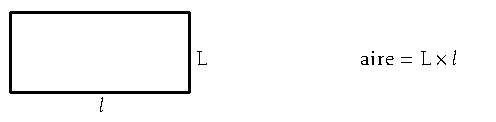
\includegraphics{pics_rectangle-plein}
  \end{center}\pause{}
  
  \begin{center}
    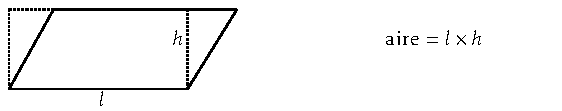
\includegraphics{pics_parallelograme}
    % \psset{xunit=2.7cm,yunit=2.7cm,algebraic=true,dotstyle=o,dotsize=3pt 0,linewidth=0.8pt,arrowsize=3pt 2,arrowinset=0.25}
    % \begin{pspicture*}(-1.09,0.7)(2.42,1.38) \psline(-0.76,1.33)(0.39,1.33) \psline(0.39,1.33)(0.08,0.83) \psline(0.08,0.83)(-1.04,0.83) \psline(-1.04,0.83)(-0.76,1.33) \rput[tl](-0.48,0.82){$l$} \psline[linestyle=dashed,dash=1pt 1pt](-1.04,0.83)(-1.04,1.33) \psline[linestyle=dashed,dash=1pt 1pt](-0.76,1.33)(-1.04,1.33) \rput[tl](-0.02,1.2){$h$} \rput[tl](1.32,1.2){aire = $l \times h$} \psline[linestyle=dashed,dash=1pt 1pt](0.08,0.83)(0.08,1.33)
    % \end{pspicture*}
  \end{center}\pause{}

  \begin{center}
    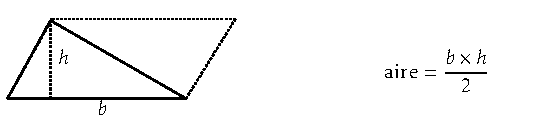
\includegraphics{pics_triangle}
    % \psset{xunit=2.7cm,yunit=2.7cm,algebraic=true,dotstyle=o,dotsize=3pt 0,linewidth=0.8pt,arrowsize=3pt 2,arrowinset=0.25}
    % \begin{pspicture*}(-1.08,0.69)(2.42,1.44) \psline[linestyle=dashed,dash=1pt 1pt](-0.76,1.33)(0.39,1.33) \psline[linestyle=dashed,dash=1pt 1pt](0.39,1.33)(0.08,0.83) \psline[linestyle=dashed,dash=1pt 1pt](0.08,0.83)(-1.04,0.83) \psline[linestyle=dashed,dash=1pt 1pt](-1.04,0.83)(-0.76,1.33) \rput[tl](-0.48,0.82){$b$} \rput[tl](-0.72,1.14){$h$} \rput[tl](1.32,1.14){aire = $\displaystyle{\frac{b \times h}{2}}$} \psline(-0.77,1.32)(0.08,0.83) \psline(0.08,0.83)(-1.04,0.83) \psline(-1.04,0.83)(-0.77,1.32) \psline[linestyle=dashed,dash=1pt 1pt](-0.77,1.32)(-0.77,0.83)
    % \end{pspicture*}
  \end{center}
\end{frame}

\begin{frame}{Figures courbes}
Pour un disque : comment obtenir $\pi r^2$, où \(r\) est le rayon ?\pause{}

Comment faire pour l'aire sous l'arc de parabole d'équation \(y = 1 - x^{2}\) ?\pause{} 
\begin{center}
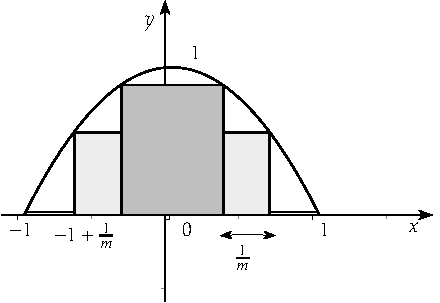
\includegraphics{pics_parabole}
% \psset{xunit=2.5cm,yunit=2.5cm,algebraic=true,dotstyle=o,dotsize=3pt 0,linewidth=0.8pt,arrowsize=3pt 2,arrowinset=0.25}
% \begin{pspicture*}(-1.11,-0.59)(1.81,1.45)
% \psaxes[labelFontSize=\scriptstyle,xAxis=true,yAxis=true,labels=none,Dx=1,Dy=1,ticksize=-2pt 0,subticks=2]{->}(0,0)(-1.11,-0.59)(1.81,1.45)]

% \pspolygon[linestyle=none,fillstyle=solid,fillcolor=lightgray,opacity=1](-0.34,0.88)(0.35,0.88)(0.35,0)(-0.34,0)

% \pspolygon[linestyle=none,fillstyle=solid,fillcolor= lightgray,opacity=0.3](-0.34,0.56)(-0.66,0.56)(-0.66,0)(-0.34,0)

% \pspolygon[linestyle=none,fillstyle=solid,fillcolor= lightgray,opacity=0.3](0.35,0.56)(0.66,0.56)(0.66,0)(0.35,0)

% \psplot[plotpoints=200]{-1.0}{1.0}{-x^2+1}
% \psline(0.35,0.88)(-0.34,0.88)
% \psline(-0.34,0.88)(0.35,0.88)
% \psline(0.35,0.88)(0.35,0)
% \psline(0.35,0)(-0.34,0)
% \psline(-0.34,0)(-0.34,0.88)
% \psline(-0.34,0.56)(-0.66,0.56)
% \psline(-0.66,0.56)(-0.66,0)
% \psline(-0.66,0)(-0.34,0)
% \psline(-0.34,0)(-0.34,0.56)
% \psline(0.35,0.56)(0.66,0.56)
% \psline(0.66,0.56)(0.66,0)
% \psline(0.66,0)(0.35,0)
% \psline(0.35,0)(0.35,0.56)
% \rput[tl](0.12,1.15){$1$}
% \rput[tl](1,-0.05){$1$}
% \rput[tl](0.42,-0.2){$\frac{1}{m}$}
% \rput[tl](0.06,-0.05){$0$}
% \rput[tl](-0.80,-0.05){$-1 + \frac{1}{m}$}
% \rput[tl](-1.1,-0.05){$-1$}
% \psline[linewidth=0.4pt]{->}(0.51,-0.13)(0.7,-0.14)
% \psline[linewidth=0.4pt]{->}(0.51,-0.13)(0.33,-0.14)
% \psline(0.66,0.02)(0.98,0.02)
% \psline(-0.66,0.02)(-1,0.02)
% \rput[tl](-0.19,1.35){$y$}
% \rput[tl](1.6,-0.05){$x$}
% \end{pspicture*}
\end{center}
Pour chaque valeur de \(m\) donnée, nous pouvons calculer l'aire de la réunion des rectangles dessinés dans cette figure\pause{} et, prenant la limite lorsque \(m \to \infty\), nous pouvons espérer obtenir une valeur pour l'aire.\pause{} Cette valeur sera notée \(\int_{-1}^{1} (1 - x^{2}) \D x\).\pause{}
\end{frame}

\subsection{Définition et propriétés}
\begin{frame}
  \begin{block}{\og Définition\fg{}}
    Soit $a,b$ deux nombres réels avec $a<b$ et $f: [a,b] \to \RR$ une fonction continue.\pause{} Nous allons noter
    \begin{equation*}
      \int_a^b f(x) \, \D x
    \end{equation*}
    l'\Defn{aire \onslide<+(5)->{algébrique}} de la surface comprise entre
    \begin{itemize}\pause{}
    \item l'axe des abcisses,\pause{}
    \item le graphe de $f$, et\pause{}
    \item les deux droites d'équations respectives $x=a$ et $x=b$.
    \end{itemize}\pause{}
  \end{block}
    \begin{center}
      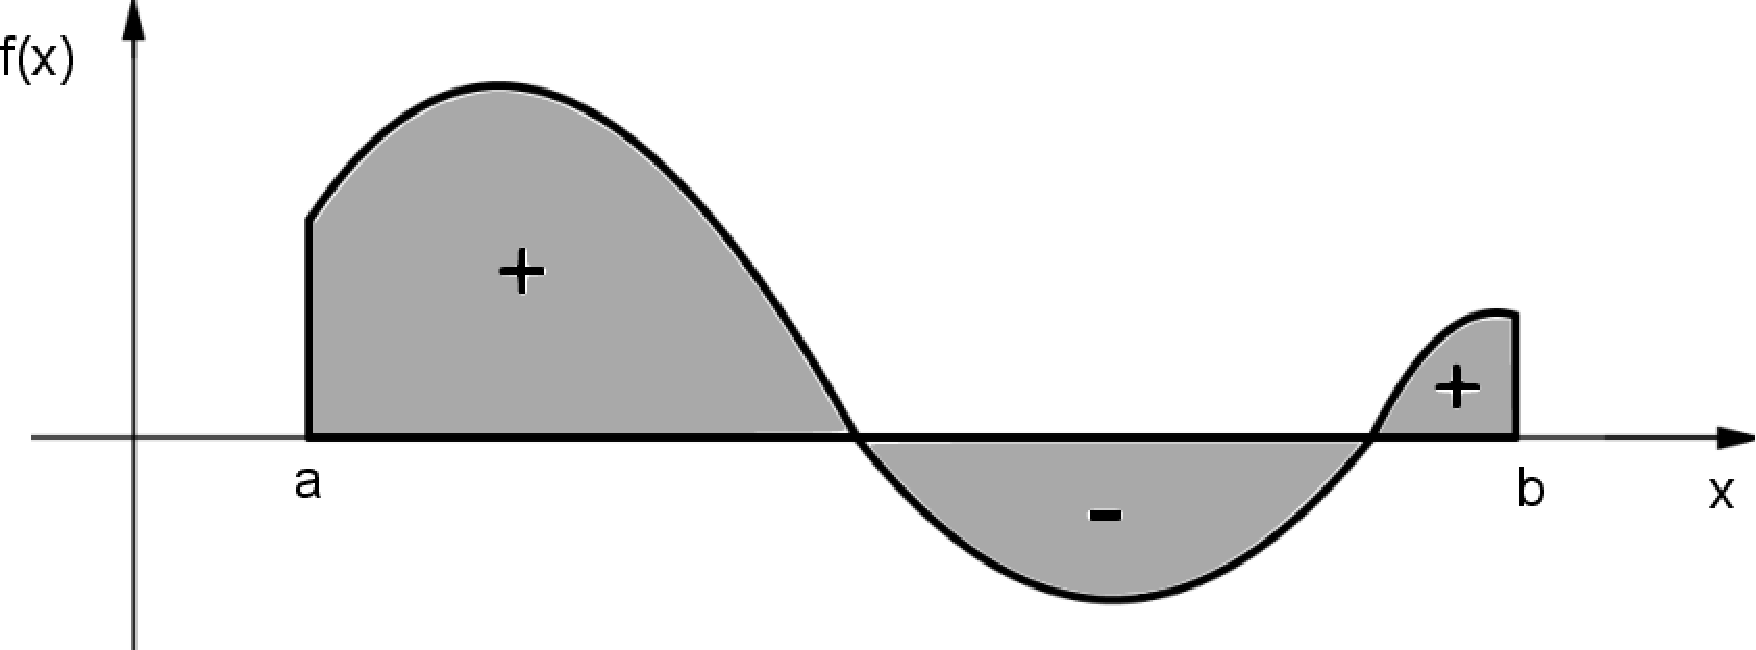
\includegraphics[height=3cm]{Fig_203}
    \end{center}
\end{frame}
\begin{frame}[fragile]{Comment faire ?}\pause{}
  \begin{tikzpicture}
\def\GraphAndAxis{%
    \draw[->] (-3.0,0) -- (2.7,0) coordinate (x axis);
    \draw[smooth,semithick,fill=none,name path=graph,domain=-2.9:2.6]% 
    plot[id=poly] (\x,0.05*\x*\x*\x - 0.2*\x*\x - 0.2*\x + 3);} % end GraphAndAxis
      \def\UpperAndLowerBoxes#1#2#3#4#5{% #1=x_i, #2=x_(i+1),
        % #3=x s.t. f(x) = min_x f(x), 
        % #4=x s.t. f(x) = max_x f(x),
        % #5= index 
        \path[name path=upward at max x] (#4,0.0) -- (#4,3.1);
        \path[name intersections={of=graph and upward at max x, by=maxf}];
        \draw[fill=gray!30] (#1,0.0) rectangle (#2,0.0 |- maxf);
        \path[name path=upward at min x] (#3,0.0) -- (#3,3.1);
        \path[name intersections={of=graph and upward at min x, by=minf}];
        \draw[fill=gray!50] (#2,0.0 |- minf) rectangle (#1,0.0)
        node[below,opacity=1.0] {\smaller{\ensuremath{x^{\phantom{*}}_{#5}}}};
      } % end UpperAndLowerBoxes
      \GraphAndAxis
      \UpperAndLowerBoxes{-2.8}{-1.3}{-2.8}{-1.3}{0}
      \UpperAndLowerBoxes{-1.3}{0.2}{-1.3}{-0.4305}{1}
      \UpperAndLowerBoxes{0.2}{1.3}{1.3}{0.2}{2}
      \UpperAndLowerBoxes{1.3}{2.5}{2.5}{1.3}{3}
      \GraphAndAxis
      \begin{scope}
        \path (2.5,1.0) -- (2.5,0.0) node [below] {\smaller\ensuremath{x^{\phantom{*}}_{4}}}; %ugly manual hack
      \end{scope}
    \end{tikzpicture}
\end{frame}
\begin{frame}
  Avant de formuler une vraie définition de l'aire algébrique, faisons quelques autres définitions.\pause{}

\begin{definition}
  Une \Defn{subdivision} \(\sigma\) d'ordre \(n\in \NN\) de l'intervalle $[a,b]$\pause{} est un choix de $n+1$ points $x_i$ ($i=0,1, \ldots, n$) tels que
  \begin{equation*}
    a=x_0 < x_1 < x_2 < \ldots < x_n=b.
  \end{equation*}
\end{definition}\pause{}
\begin{center}
  \includegraphics{subdivision}
  % \psset{xunit=3.0cm,yunit=4.0cm,algebraic=true,dotstyle=o,dotsize=3pt 0,linewidth=0.8pt,arrowsize=3pt 2,arrowinset=0.25}
  % \begin{pspicture*}(0.30,-0.49)(4.81,0.27) \psaxes[labelFontSize=\scriptstyle,xAxis=true,yAxis=false,labels=none,Dx=1,Dy=1,ticksize=0pt 0,subticks=2]{->}(0,0)(0.52,-0.49)(4.81,0.27) \rput[tl](4.7,-0.06){$x$}
  %   \psdots[dotstyle=|](0.68,0) \rput[b](0.55,0.02){$a=x_0$}
  %   \psdots[dotstyle=|](0.95,0) \rput[b](0.95,0.02){$x_1$}
  %   \psdots[dotstyle=|](1.5,0) \rput[b](1.5,0.02){$x_2$}
  %   \psline{<->}(0.95,-0.1)(1.5,-0.1) \rput(1.225,-0.15){calibre}
  %   \psdots[dotstyle=|](1.72,0) \rput[b](1.72,0.02){$x_3$}
  %   \psdots[dotstyle=|](2.13,0)
  %   \psdots[dotstyle=|](2.26,0)
  %   \psdots[dotstyle=|](2.65,0) \rput[b](2.65,0.02){$x_{i}$} \psdots[dotstyle=|](3.1,0)
  %   \psdots[dotstyle=|](3.5,0) \rput[b](3.5,0.02){$x_{n-2}$}
  %   \psdots[dotstyle=|](4,0) \rput[b](4,0.02){$x_{n-1}$}
  %   \psdots[dotstyle=|](4.5,0) \rput[b](4.5,0.02){$x_n = b$}
  % \end{pspicture*}
\end{center}\pause{}
\begin{definition}
  Le \Defn{calibre} de la subdivision $\sigma$ est\pause{}
  \begin{math}
    \max_{i=1,2, \ldots,n} \abs{x_i - x_{i-1}}.
  \end{math}
\end{definition}
\end{frame}
%\asyinclude{subdivision.asy}

\begin{frame}% FIXME: intégrer au syllabus dans sa version reformulée ?
  Pour une subdivision \(\sigma\) donnée, on considère
  \begin{itemize}
  \item \(m_{i} = \inf \set{ f(x) \telque x\in \intercc{x_{i-1},x_{i}}}\)\pause
  \item la \Defn{somme de Darboux inférieure} \(s(\sigma)\)\pause
    \begin{equation*}
      s(\sigma) = \sum_{i=1}^n m_{i} (x_i - x_{i-1})
    \end{equation*}
  \end{itemize}\pause{}
  et similairement~: 
  \begin{itemize}
  \item \(M_{i} = \max \set{ f(x) \telque x\in \intercc{x_{i-1},x_{i}}}\).\pause{}
  \item La somme de Darboux \Defn{supérieure} \(S(\sigma)\) :\pause{}
    \begin{equation*}
      S(\sigma) = \sum_{i=1}^n M_{i} (x_i - x_{i-1})
    \end{equation*}
  \end{itemize}
\end{frame}

\begin{frame}% FIXME: intégrer au syllabus dans sa version reformulée ?
  On peut démontrer :\pause{}
  \begin{proposition}Pour toute fonction \(f : [a,b]\to \RR\) :
    \begin{multline*}
      \sup \set{s(\sigma) \telque \sigma \text{ subdivision de \([a,b]\)}}\pause
      \\\leq \inf  \set{S(\sigma) \telque \sigma \text{ subdivision de \([a,b]\)}}
    \end{multline*}
  \end{proposition}\pause{}
  
  \begin{definition}
    Lorsque l'inégalité ci-dessus est une égalité,\pause{} alors on note
    \begin{equation*}
      \int_{a}^{b} f \quad \text{ou} \quad \int_a^b f(x) \, \D x
    \end{equation*}
    le nombre commun\pause{}, et on l'appelle \og intégrale de Riemann de \(f\)\fg{} ou \og intégrale définie de \(f\)\fg{} entre \(a\) et \(b\).
  \end{definition}
\end{frame}
\begin{frame}
\begin{proposition}
  Si \(f : \intercc{a,b} \to \RR\) est continue, alors \(\int_{a}^{b} f\) existe.
\end{proposition}
%% FIXME: un peu de blabla autour + faire le cas des fonctions monotones bornées (pas forcément continues). cf ~/Téléchargements/Cours-7-Integrale-de-Riemann.pdf sur LDLC pour une illustration efficace.
\end{frame}
\begin{frame}{Échange des bornes}
  \begin{definition}
    Lorsque $\int_a^b f(t) \, \D t$ existe\pause{}, on note
    \begin{equation*}
      \int_b^a f(t) \, \D t= - \int_a^b f(t) \, \D t.
    \end{equation*}\pause{}
  \end{definition}
  \begin{remark}
    En d'autres termes : renverser les bornes change le signe.
  \end{remark}
\end{frame}

\subsection{Quelques résultats}
\begin{frame}{Propriété d'additivité}\pause{}
  \begin{proposition}
    Pour $c \in \RR$, si deux des trois intégrales suivantes existent, la troisième existe aussi et
    \begin{equation*}
      \int_a^b f(t) \, \D t= \int_a^c f(t) \, \D t + \int_c^b f(t) \, \D t.
    \end{equation*}\pause{}
    Ceci est l'\Defn{additivité par rapport au domaine d'intégration}.
  \end{proposition}
\end{frame}

\begin{frame}
  \begin{proposition}
    Soient \(f\) et \(g\) des fonctions avec \(f(x) \leq g(x)\) pour tout \(x \in [a,b]\).\pause{}

    Considérons le sous-ensemble $D$ du plan :
    \begin{center}
      \includegraphics[width=3cm]{Fig_200}
    \end{center}\pause{}
    c'est-à-dire :
    \begin{equation*}
      D= \set{ (x,y) \in \RR^2 \telque x \in [a,b] \mbox{ et } f(x) \leq y \leq g(x) }
    \end{equation*}\pause{}

    Si les deux intégrales définies suivantes existent, l'aire de $D$ est
    \begin{equation*}
      \int_a^b g(x) \, \D x - \int_a^b f(x) \, \D x.
    \end{equation*}
  \end{proposition}
\end{frame}

\begin{frame}
  \begin{proposition}
    Si $f$ et $g$ sont deux fonctions intégrables sur l'intervalle $[a,b]$ et si $\alpha, \beta \in {\RR}$, alors
    \begin{equation*}
      \int_a^b (\alpha f+ \beta g)(x) \, \D x = 
      \alpha \int_a^b f(x) \, \D x + \beta \int_a^b g(x) \, \D x.
    \end{equation*}
  \end{proposition}
\end{frame}

\begin{frame}
  \begin{proposition}
    Soit $f$ une fonction réelle sur $[a,b]$ vérifiant avec $f(x) \geq 0$ pour tout $x$ de $[a,b]$. Alors
    \begin{equation*}
      \int_a^b f(x) \, dx \geq 0.
    \end{equation*}\pause{}
    Si \(f\) est \emph{de plus} continue, nous avons l'équivalence~:\pause{}
    \begin{equation*}
      \int_a^b f(x) \, dx = 0 \quad \iff \quad \forall x \in [a,b] : f(x)=0.
    \end{equation*}
  \end{proposition}

  \begin{corollary}
    En particulier, si \(f(x) \leq g(x)\) pour tout \(x \in [a,b]\), alors \(\int_{a}^{b} f \leq \int_{a}^{b} g\).
  \end{corollary}
\end{frame}

\subsection{Théorème fondamental}
\label{se:11:theoreme-fondamental}
\begin{frame}
  Soit \(f : [a,b] \to \RR\) une fonction continue. Définissons :
  \begin{equation*}
    F(x) = \int_a^x f(t) \, \D t
  \end{equation*}\pause{}
  La dérivée de cette fonction \(F\) au point \(x_{0}\) est donnée par~:
  \begin{align*}
    \uncover<+->{F'(x_0) &= \limite x {x_{0}} \frac{\int_a^x f(t) \, \D t - \int_a^{x_0} f(t) \, \D t}{x-x_0}\\}
    \uncover<+->{&= \limite x {x_{0}} \frac{\int_{x_{0}}^{x} f(t) \D t}{x - x_0}}
  \end{align*}\pause{}
  \begin{center}
    \includegraphics[height=4cm]{pics_thm-fond}
  \end{center}
\end{frame}

\begin{frame}
  \begin{theorem}[Théorème fondamental du calcul différentiel et intégral]\pause{}
    Soit $f$ une fonction continue sur l'intervalle $\interoo{c,d}$, et soit $a$ un point de $\interoo{c,d}$. Alors\pause{}
    \begin{equation*}
      F : \interoo{c,d} \rightarrow {\RR} : x \mapsto \int_a^x f(t) \, \D t
    \end{equation*}
    est l'unique primitive de $f$\pause{} qui s'annule en \(x = a\).\pause{}
  \end{theorem}\pause{}

  \begin{corollary}\pause{}
    Si \(G\) une primitive quelconque de \(f\),\pause{} alors \(G(x) - G(a)\) est une primitive de \(f\)\pause{} s'annulant en \(a\), et donc :\pause{}
    \begin{equation*}
      \int_{a}^{x} f(t) \D t = G(x) - G(a) \pause= \sqbracket[\Big]{G(t)}_{t=a}^{t=x}
    \end{equation*}
  \end{corollary}\pause{}

  \begin{remark*}
    Ceci fournit un moyen de calculer le membre de gauche à condition d'avoir à disposition une primitive de \(f\).
  \end{remark*}
\end{frame}

\subsection{Intégration définie et indéfinie}
\begin{frame}
  Au vu du théorème fondamental, les formules de recherche de primitive admettent des variantes applicables au calcul d'intégrales définies.\pause{} En particulier, pour le changement de variable\pause{} : en posant $t=g(x)$~:
  \begin{equation*}
    \int_a^b f(g(x)) \cdot g'(x) \, \D x\pause = \int_{t_1}^{t_2} f(t) \, \D t
  \end{equation*}\pause{}
  où $t_1=g(a)$ et $t_2=g(b)$.
\end{frame}

\begin{frame}
\begin{example}
  Soit à calculer
  \begin{equation*}
    I= \int_0^2 \sin (3x+5) \, \D x.
  \end{equation*}\pause{}
  En posant $t=3x+5$,\pause{} nous avons $\D t=3 \, \D x$.\pause{} Dès lors~:
  \begin{align*}
    \uncover<+->{I &= \frac{1}{3} \int_5^{11} \sin t \, \D t \\}
    \uncover<+->{&=\frac{1}{3} \left[ - \cos t \right]_5^{11} = \frac{1}{3}(- \cos 11+ \cos 5).}
  \end{align*}
\end{example}\pause{}
\begin{example}
  Autre approche : on calcule une primitive de \(\sin{(3x+5)}\)~:
  \begin{equation*}
    \int \sin(3x+5) \D{x}\pause = \frac{1}{3}\int \sin(t)\D{t}\pause = - \frac{1}{3}\cos(t)\pause = - \frac13\cos(3x+5)
  \end{equation*}\pause{}
  et on en déduit le même résultat :
  \begin{equation*}
    \int_{0}^{2} \sin(3x+5) \D{x} \pause =  \sqbracket[\big]{- \frac13\cos(3x+5)}_{0}^{2} \pause= - \frac{1}{3}\cos(11) + \frac{1}{3} \cos(5).
  \end{equation*}
\end{example}
\end{frame}

\subsection{Intégrales généralisées}
\begin{frame}
  Dans la définition de l'intégrale définie de Riemann
  \begin{equation*}
    \int_a^b f(x) \, dx,
  \end{equation*}
  nous avons supposé\pause{}
  \begin{itemize}
  \item $a,b \in \RR$, et\pause{}
  \item $f$ est fonction continue sur $[a,b]$.
  \end{itemize}\pause{}
  Les applications requièrent (au moins) deux généralisations de ce concept~:\pause{}
  \begin{itemize}
  \item lorsque $f$ est définie sur \(\interoo{a,b}\), et\pause{}
  \item lorsque $a$ ou $b$ est infini.
  \end{itemize}
\end{frame}

\subsubsection{Cas d'une fonction non bornée}
\begin{frame}
  \begin{definition}
    Pour une fonction $f$ continue sur $\interco{a,b}$, nous posons
    \begin{equation*}
      \int_a^b f(x) \, \D x =\pause{} \limite[<] u b \int_a^u f(x) \, \D x.
    \end{equation*}
    si cette limite existe.\pause{} Lorsque la limite est réelle, on dit que l'intégrale converge.\pause{}
  \end{definition}
  On procède similairement pour une fonction définie et continue sur \(\interoc{a,b}\).
\end{frame}

\begin{frame}{Exemple}
  \begin{tabular}{p{.55\linewidth{}}c}
    \begin{minipage}{1.0\linewidth}
      \begin{example}
        Considérons \(\interoc{0,1} \to \RR : x \mapsto \frac{1}{x}\)\pause{}
        \begin{multline*}
          \uncover<+->{\limite[>] {u} {0} \int_u^1 \frac{1}{x} \, \D x \\}%
          \uncover<+->{= \limite[>] {u} {0} \ln(1) - \ln(u)}%
          \uncover<+->{= + \infty}
        \end{multline*}\pause{}
        Donc l'intégrale ne converge pas\pause{}, plus précisément elle tend vers $+ \infty$.\pause{}
      \end{example}
    \end{minipage}
    & \raisebox{-.5\height}{\includegraphics[height=7cm]{Fig_215_2}}
  \end{tabular}
\end{frame}

\begin{frame}
  \begin{example}
    Soit \(a\) un nombre réel, avec \(a > 0\) et \(a \neq 1\).\pause{} Considérons la fonction
    \begin{equation*}
      f_{a} : \interoc{0,1} \rightarrow \RR : x \mapsto \frac{1}{x^{a}}
    \end{equation*}\pause{}
    Alors
    \begin{equation*}
      \limite[>] {u} {0} \int_u^1 \frac{1}{x^{a}} \, \D x \pause= \frac{1}{1 - a} \limite[>] {u} {0} \paren*{1 - u^{1-a}}
    \end{equation*}\pause{}
    Donc :
    \begin{itemize}\pause{}
    \item Si \(a < 1\), alors l'intégrale vaut \(\frac{1}{1-a}\), tandis que\pause{}
    \item si \(a \geq 1\), l'intégrale ne converge pas (le cas \(a = 1\) ayant été fait ci-dessus.)
    \end{itemize}
  \end{example}
\end{frame}

% \begin{frame}
%   \begin{definition}
%     Lorsque le point $c$ près duquel $f$ n'est pas bornée est intérieur à l'intervalle d'intégration, nous posons
%     \begin{equation*}
%       \int_a^b f(x) \, \D x = \limite [<] u c \int_a^u f(x) \, \D x + \limite[>] v c \int_v^b f(x) \, \D x;
%     \end{equation*}
%     et l'intégrale ainsi définie converge à condition que les deux limites convergent dans ${\RR}$.
%   \end{definition}
%   Cette définition se généralise au cas d'une fonction bornée sauf aux voisinages d'un nombre fini de points de l'intervalle d'intégration (il suffit de décomposer cet intervalle en sous-intervalles dont chacun ne contient qu'un seul point exceptionnel).
% \end{frame}

\subsubsection{Cas d'un domaine non borné}
\begin{frame}
  \begin{definition}
    Lorsqu'on considère une fonction $f: \interco{a,+\infty} \to \RR$ continue, nous posons\pause{}
    \begin{equation*}
      \int_a^{+\infty}\,f(x)\D{x}= \limite T {+\infty} \int_a^T \,f(x)\D{x}
    \end{equation*}
    si cette dernière limite existe.\pause{} Lorsque la limite est réelle, on dit que l'intégrale converge.
  \end{definition}
\end{frame}
\begin{frame}
  \begin{example}
    Soit
    \begin{equation*}
      f : \interco{1,+\infty} \to {\RR} : x \mapsto \frac{1}{x}.
    \end{equation*}\pause
    Alors
    \begin{align*}
      \limite T {+\infty} \int_1^T \dfrac{1}{x} \, \D x\pause =  \limite T {+\infty} \ln(T) - \ln(1)\pause =  + \infty.
    \end{align*}\pause{}
    L'intégrale diverge vers $+ \infty$.
  \end{example}
\end{frame}
\begin{frame}
  Ainsi, la surface ombrée sur le graphique\pause{}
  \begin{center}
    \includegraphics[scale=0.3]{Fig_217_1}
  \end{center}\pause{}
  est d'aire infinie.
\end{frame}
\begin{frame}
  \begin{exercise}
    Soit \(a\) un nombre réel, avec \(a > 0\) et \(a \neq 1\). Considérons la fonction
    \begin{equation*}
      f_{a} : \interco{1,\infty} \rightarrow {\RR} : x \mapsto \frac{1}{x^{a}}
    \end{equation*}\pause{}
    Prouvez \pause{}: fonction est intégrable sur \(\interco{1,\infty}\) si et seulement si \(a > 1\).
  \end{exercise}
\end{frame}
\course{16} % courbes / fonctions d'une variable à valeurs vectorielles
\section{Fonctions d'une variable réelle à valeurs vectorielles}
\begin{frame}
\begin{definition}
  Une \emph{fonction d'une variable réelle à valeurs vectorielles} est une fonction de la forme \(f : A \subset \RR \to \RR^{n}\).\pause{}
\end{definition}

  On imagine qu'une telle fonction décrit la paramétrisation d'une courbe, d'une trajectoire.\pause{} À chaque valeur de la variable \(t\in A\) correspond un point \(f(t)\in \RR^n\). Lorsque \(t\) évolue, cela rend compte du déplacement du point.\pause{}

  La valeur de \(n\) indique dans quel espace la courbe \og vit\fg{} :\pause{}
  \begin{itemize}
  \item Si \(n = 1\), le mobile se déplace le long d'une droite ;\pause{}
  \item si \(n = 2\), le mobile se déplace dans un plan ;\pause{}
  \item si \(n = 3\), le mobile se déplace dans l'espace,
  \item etc.
  \end{itemize}
\end{frame}

\begin{frame}
  \begin{example}Dans les exemples ci-dessous, c'est l'ensemble image \(\Im f\) qui est représenté.\pause{} Ce n'est \emph{pas} le graphe de \(f\)\pause{} : il n'a pas d'interprétation utile à ce stade.\pause{}
    \begin{center}
      \begin{tabular}{ccc}
        \uncover<+->{\begin{minipage}{0.30\linewidth}
            \includegraphics[width=\linewidth]{courbe-droite}
          \end{minipage}}%
        & \uncover<+(1)->{\begin{minipage}{0.30\linewidth}
            \includegraphics[width=\linewidth]{courbe-cercle}
          \end{minipage}}\\
        \uncover<+(-1)->{\mbox{\(f : \intercc{-1,1} \to \RR : t \mapsto (t,t)\)}}%
        & \uncover<+->{ \mbox{\(f : \intercc{-\pi, \sfrac\pi2} \to \RR : t \mapsto (\cos t,\sin t)\)}}
      \end{tabular}
    \end{center}
  \end{example}
\end{frame}

\begin{frame}
  \begin{center}
    \uncover<2->{\includegraphics[width=6cm]{courbe-spirale}}
  \end{center}
  \begin{align*}
    f : \intercc{-5\pi, 3\sfrac\pi2} \to \RR : t \mapsto \paren{t^{2} \cos t, t^{2} \sin t}
  \end{align*}\pause{}

  \begin{remark}\pause{}
    Notons que l'ensemble \(\Im f\) ne donne pas une information suffisante pour pouvoir connaître le mouvement. Deux courbes peuvent provenir de deux paramétrisations différentes.
  \end{remark}
\end{frame}
\begin{frame}
  
\end{frame}
\subsection{Régularité}
\begin{frame}{Limites et continuité}
  \begin{definition}
    Soit \(f : A \subset \RR \to \RR^{n}\) une application, \(a \in A\), et \(\point L \in \RR^{n}\).\pause{}
    On dit que la limite de \(f\) en \(a\) est \(\point L\) si\pause{}
    \begin{equation*}
      \forall \epsilon > 0, \exists \delta  > 0 : \forall x \in A, \abs{x-a} < \delta \Rightarrow \norme{f(x)-\point L} \leq \epsilon.
    \end{equation*}\pause{}
    On écrit dans ce cas
    \begin{equation*}
      \limite x a f(x) = L.
    \end{equation*}\pause{}
  \end{definition}
  \begin{definition}
    La fonction \(f : A \subset \RR \to \RR^{n}\)\pause{} est \Defn{continue} en \(a\in A\) si\pause{}
    \begin{equation*}
      \limite x a f(x) = f(a).
    \end{equation*}\pause{}
    La fonction \(f\) est dite \Defnemph{continue} si elle est continue en chaque point.
  \end{definition}
\end{frame}
\begin{frame}
  \begin{definition}
    Une application \(f : A \subset \RR \to \RR\) est \Defn{dérivable} en \(a \in A\) si\pause{} \(a\) est intérieur à \(A\) et\pause{} si la limite
    \begin{equation*}
      \limite x a \frac{f(x)-f(a)}{x-a}
    \end{equation*}
    existe. \pause{}Dans ce cas, cette limite est notée \(f'(a)\) est appelée la \Defnemph{dérivée} de \(f\) en \(a\).
  \end{definition}\pause{}

  En pratique, nous avons le résultat suivant :\pause{}
  \begin{proposition}
    Une application \(f : A \subset \RR \to \RR^{n}\) est continue\pause{} (resp. dérivable)\pause{} en \(a \in A\)\pause{} si et seulement si pour tout \(i = 1 \ldots n\), \(f_{i} : A \to \RR\) est continue (resp. dérivable) en \(a\).\pause{} De plus, si elle existe, la dérivée est donnée par
    \begin{equation*}
      f'(a) = (f_{1}'(a), \ldots,f_{n}'(a)).
    \end{equation*}
  \end{proposition}
\end{frame}

\subsection{Courbes}
\begin{frame}
  \begin{definition}
    Une \Defn{courbe paramétrée} de \(\RR^{n}\)\pause{} est une application continue
    \begin{equation*}
      \gamma : I \subset \RR \to \RR^{n}
    \end{equation*}
    définie sur un intervalle \(I\).
  \end{definition}\pause{}

  \begin{remark*}
    Si \(\gamma\) est une courbe paramétrée dérivable correspondant à la trajectoire d'un mobile \alert<.(1)>{au cours du temps}\pause{}, alors \(\gamma'(t)\) correspond au \emph{vecteur vitesse} de ce mobile à l'instant \(t\).\pause{} La \emph{vitesse scalaire} est \(\norme{\gamma'(t)}\).
  \end{remark*}
  \begin{exercise}\pause{}
      Représenter l'image de \(\gamma\), où \(\gamma(t) = (\cos(t), t)\). Représenter également \(\gamma'(t)\) pour quelques valeurs de \(t\). 
  \end{exercise}
\end{frame}
\frame{\includegraphics{courbe-costt}}

\subsubsection{Re-paramétrisation}
\label{sec:courbes}
\begin{frame}
  \begin{remark*}
    Intuitivement, on peut parcourir une courbe donnée de plusieurs manières :
    \begin{itemize}
    \item dans un sens ou dans l'autre,
    \item ou à différentes vitesses.
    \end{itemize}
  \end{remark*}\pause{}
  \begin{definition}
    Si \(\gamma : I \to \RR^{n}\) est une courbe paramétrée, on dit qu'une courbe paramétrée \(\eta : J \to \RR^{n}\) est une \Defn{re-paramétrisation} de \(\gamma\) si\pause{} il existe une bijection continue \(\alpha : I \to J\) telle que \(\eta \circ\alpha = \gamma\).\pause{}

    On dit que \(\gamma\) et \(\eta\) ont \emph{même orientation} si l'application \(\alpha\) est croissante.
  \end{definition}
\end{frame}

\begin{frame}
\begin{remark*}
  \begin{itemize}
  \item Certaines notions, telle que la longueur d'une courbe, devraient idéalement ne pas dépendre de la paramétrisation choisie.\pause{}
  \item D'autres notions en dépendent de manière évidente, comme par exemple la notion de vitesse.\pause{}
  \end{itemize}
\end{remark*}
\end{frame}
% FIXMELATER: parler de conserver ou changer l'orientation.
% cf Chap11.tex

\subsubsection{Vitesse et vecteur tangent}
\label{sec:vitesse}
\begin{frame}
\begin{definition}
  Le \Defn{vecteur vitesse} ou \Defn{vecteur tangent} d'une courbe paramétrée \(\gamma\) à l'instant \(t\) est donné par le vecteur \(\gamma'(t)\).\pause{} Sa norme est parfois appelée la \Defn{vitesse numérique} à l'instant \(t\).\pause{} Le vecteur  \(\frac{\gamma'(t)}{\norme{\gamma'(t)}}\) est appelé \Defn{vecteur tangent unitaire} à l'instant \(t\) et est noté \(T(t)\).
\end{definition}
\end{frame}
% \begin{frame}
%   \begin{example}
%     \begin{center}
%       \begin{tabular}{ccc}
%         \uncover<+->{        \begin{minipage}{0.30\linewidth}
%           \includegraphics[width=\linewidth]{courbe-droite-tg-nonunit}
%         \end{minipage}
% }        \uncover<+->{        & \begin{minipage}{0.30\linewidth}
%           \includegraphics[width=\linewidth]{courbe-parabola-tg-nonunit}
%         \end{minipage}
%                                }\uncover<+->{        & \begin{minipage}{0.30\linewidth}
%           \includegraphics[width=\linewidth]{courbe-spirale-tg-nonunit}
%         \end{minipage}
%  }     \end{tabular}
%     \end{center}
%   \end{example}
% \end{frame}
\begin{frame}
  \begin{example}
    \begin{center}
      \begin{tabular}{ccc}
        \uncover<+->{        \begin{minipage}{0.30\linewidth}
          \includegraphics[width=\linewidth]{courbe-droite-tg}
        \end{minipage}
}        \uncover<+->{        & \begin{minipage}{0.30\linewidth}
          \includegraphics[width=\linewidth]{courbe-parabola-tg}
        \end{minipage}
                               }\uncover<+->{        & \begin{minipage}{0.30\linewidth}
          \includegraphics[width=\linewidth]{courbe-spirale-tg}
        \end{minipage}
 }     \end{tabular}
    \end{center}
  \end{example}
\end{frame}
\subsubsection{Accélération et vecteur normal}
\label{sec:acceleration}
\begin{frame}
\begin{definition}
Le \Defn{vecteur accélération} de \(\gamma\) à l'instant \(t\) est défini par \(\gamma''(t)\).%\pause{} Sa norme est parfois appelée l'\Defn{accélération numérique} à l'instant \(t\).
\end{definition}\pause{}
Attention à la définition similaire mais différente suivante, où on dérive maintenant le vecteur tangent unitaire :
\begin{definition}
  Le \Defn{vecteur normal unitaire}, s'il existe, est donné par \( N(t) = \frac{T'(t)}{\norme{T'(t)}}\).
\end{definition}
\end{frame}

\begin{frame}
  \begin{remark*}
    Le vecteur normal unitaire est effectivement normal (orthogonal) au vecteur tangent.
  \end{remark*}\pause{}
  \begin{proof}
    Puisque \(T(t)\) est de norme \(1\),\pause{} on peut dériver l'égalité
    \begin{equation*}
      \scalprod{T(t)}{T(t)} = 1
    \end{equation*}\pause
    pour obtenir
    \begin{equation*}
      2 \scalprod{T'(t)}{T(t)} = 0
    \end{equation*}\pause{}
    ce qui, en divisant par \(2\) et par la norme de \(T'\), donne bien \(\scalprod{N(t)}{T(t)} = 0\) comme attendu.
  \end{proof}
\end{frame}

\begin{frame}
  \begin{minipage}{0.30\linewidth}
    \includegraphics[width=\linewidth]{courbe-spirale-norm}
  \end{minipage}
\end{frame}

\subsubsection{Vecteur binormal}
\label{sec:vecteur-binormal}
\begin{frame}
  \begin{definition}
    Si \(n = 3\), c'est-à-dire pour une courbe dans l'espace\pause{}, on définit le \emph{vecteur binormal} \(B = T \vecprod N\).
  \end{definition}\pause{} Son utilité est la suivante~:
  \begin{proposition}
    La courbe \(\gamma\) est plane si et seulement si \(B'(t) = 0\) pour tout \(t\).
  \end{proposition}\pause{}
  \begin{definition}
    Une courbe plane est une courbe dont l'image est entièrement contenue dans un plan.
  \end{definition}
\end{frame}

\subsubsection{Longueur d'une courbe}
\label{sec:longueur-dune-courbe}
\begin{frame}
Si \(\gamma: I \to \RR^{n}\) est dérivable et si \(a, b \in I\), la \Defn{longueur} de \(\gamma([a,b])\) est donnée par l'intégrale~:
\begin{equation*}
  \int_{a}^{b} \norme{\gamma'(t)}\D t
\end{equation*}
\end{frame}

\begin{frame}
\begin{proof}[Idée de preuve]
  Prenons \(a = 0\) et \(b = 1\) pour simplifier.\pause{} Subdivisons le domaine \([a,b]\) en \(n\) parties égales,\pause{} et approchons la longueur par\pause{}
  \begin{equation*}
    \sum_{i=1}^{n} \norme{\gamma(\sfrac in) - \gamma(\sfrac{(i-1)}{n})}
\pause    =    \sum_{i=1}^{n} \frac{\norme{\gamma(\sfrac in) - \gamma(\sfrac{(i-1)}{n})}}{\sfrac1n} \;\frac 1n
  \end{equation*}\pause{}
  On remarque que lorsque \(n\) est grand, la fraction \(\frac{\norme{\gamma(\sfrac in) - \gamma(\sfrac{(i-1)}{n})}}{\sfrac1n}\)\pause{} s'approche de \(\norme{\gamma'(\sfrac in)}\), de sorte que\pause{} la somme ci-dessus correspond à l'intégrale de Riemann.
\end{proof}
\end{frame}
\course{17} % Début matrice
\section{Matrices}

\subsection{Introduction}
\begin{frame}
  Utilisations des matrices~:\pause{}
  \begin{itemize}
  \item Résolution de systèmes d'équations\pause{}
  \item Modélise des transformations simples : les \og applications linéaires\fg{}\pause{} (p.ex. rotations et symétries)\pause{}
  \item S'utilisent dans des modèles de probabilités (pensons à Google)\pause{}
  \item Ingrédient dans la résolution de systèmes d'équations différentielles\pause{}
  \item Traitement d'images\pause
  \item Tant d'autres choses...
  \end{itemize}
\end{frame}
\begin{frame}
  \begin{definition}Une \Defn{matrice réelle} de taille \(m\times n\) est un tableau rectangulaire\pause{} ayant \(m\) lignes\pause{} et \(n\) colonnes.
  \end{definition}\pause{}
  \begin{example}
    Ceci sont des matrices~:\pause{}
    \begin{equation*}
      \begin{pmatrix}
        2 & 1\\
        \pi & -4
      \end{pmatrix},\pause
      \begin{pmatrix}
        1 & 2 & 3\\
        2 & 1 & 0
      \end{pmatrix},\pause
      \begin{pmatrix}
        0 &0&0
      \end{pmatrix},\pause
      \begin{pmatrix}
        1\\ 4 \\ \textup{e}+\pi
      \end{pmatrix},\pause
      \begin{pmatrix}
        -\pi
      \end{pmatrix}
    \end{equation*}\pause{}
    \begin{equation*}
      \begin{pmatrix}
        0 & 1 & 2\\
        0 & -4 & 3\\
        0 & 0 & 5
      \end{pmatrix},\pause
      \begin{pmatrix}
        0 & 0 & 0\\
        0 & 1 & 0\\
        0 & 0 & 2
      \end{pmatrix},\pause
      \begin{pmatrix}
        0 & 0 & 0\\
        5 & 1 & 0\\
        21 & 0 & 2
      \end{pmatrix},
      \ldots
    \end{equation*}
  \end{example}
\end{frame}
\begin{frame}
  \begin{definition}Pour une matrice \(M\) de taille \(m\times n\) :
    \begin{itemize}[<+->]
    \item Si \(n = 1\), la matrice est appelée \Defn{matrice-colonne}, ou \Defn{vecteur-colonne} ;
    \item si par contre \(m = 1\), la matrice est appelée \Defn{matrice-ligne} ;
    \item si enfin \(m = n\), la matrice est appelée une \Defn{matrice carrée} ;
    \item l'élément se trouvant à l'intersection de la \(i\)\ieme{} ligne et de la \(j\)\ieme{} colonne est noté \(M_{ij}\) ;
    \item on note \(\Mat(m,n)\) ou \(\RR^{m\times n}\) l'ensemble de toutes les matrices de taille \(m \times n\).
    \end{itemize}
  \end{definition}
  \begin{example}\pause{}
    \begin{equation*}
      \begin{pmatrix}
        M_{11} &\ldots& M_{1n}\\
        \vdots& \ddots&\vdots \\
        M_{m1} &\ldots& M_{mn}\\
      \end{pmatrix}
    \end{equation*}
  \end{example}
\end{frame}
\begin{frame}
  \begin{definition}
    Deux matrices \(M\) et \(N\) sont égales si elles ont la même taille, disons \(m\times n\), et les même mêmes éléments :\pause{}
    \begin{equation*}
      M = N \iff M_{ij} = N_{ij} \quad\text{pour tout \(i = 1, \ldots, m\) et tout \(j = 1, \ldots, n\)}
    \end{equation*}
  \end{definition}\pause{}
  \begin{exercise}
    Déterminer \(x\) pour que \(M\) et \(N\) soit égales :
    \begin{equation*}
      \begin{pmatrix}
        0 & x^{2} \\
        1 & \pi
      \end{pmatrix}
      =
      \begin{pmatrix}
        0 & 1\\
        x^{4} & \pi
      \end{pmatrix}
    \end{equation*}
  \end{exercise}
  \begin{answer}\pause{}
    Il faut \(x^{2} = 1\) et \(1 = x^{4}\).\pause{} La seule possibilité est \(x = 1\).
  \end{answer}
\end{frame}

\subsection{Opérations sur les matrices}
\subsubsection{Somme}
\begin{frame}
  \begin{definition}
    Si \(M\) et \(N\) sont deux matrices \emph{de même taille}\pause{}, on définit leur somme \(M+N\) par\pause{}
    \begin{equation*}
      {(M+N)}_{ij} = M_{ij} + N_{ij}.
    \end{equation*}\pause{}
    La somme a encore la même taille que \(M\) et que \(N\).
  \end{definition}\pause{}
  \begin{example}
    \begin{equation*}
      \begin{pmatrix}
        0 & 1 \\ \sqrt 2 & \pi
      \end{pmatrix}
      +
      \begin{pmatrix}
        1 & -1 \\ 1 & 0
      \end{pmatrix}
      = \pause
      \begin{pmatrix}
        1 & 0 \\ 1 + \sqrt 2 & \pi
      \end{pmatrix}
    \end{equation*}
  \end{example}
\end{frame}
\begin{frame}{Matrice nulle}
  \begin{definition}
  Une matrice constituée uniquement de \(0\) est appelée \Defn{matrice nulle}.\pause{} On la note parfois \(0\), ou \(0_{m\times n}\) pour indiquer sa taille.
\end{definition}\pause{}
  \begin{proposition}
    La matrice nulle est neutre dans l'addition matricielle.
  \end{proposition}\pause{}
  \begin{equation*}
    \begin{pmatrix}
      1 & 2\\ 3 & 4
    \end{pmatrix}
    +
    \begin{pmatrix}
      0&0\\0&0
    \end{pmatrix}=\pause
    \begin{pmatrix}
      1 & 2\\ 3 & 4
    \end{pmatrix}
  \end{equation*}
\end{frame}
\begin{frame}
  \begin{proposition}
    La somme matricielle de deux matrices \(M\) et \(N\) de même taille est donc une opération~:
    \begin{equation*}
      + : \Mat(m,n) \times \Mat(m,n) \to \Mat(m,n)
    \end{equation*}\pause{}
    ayant les propriétés :\pause{}
    \begin{description}[<+->]
    \item[Commutativité] \(M+N = N+M\)
    \item[Associativité] \((M+N)+P = M+(N+P)\)\uncover<+->{ on écrira généralement \(M+N+P\) sans parenthèses.}
    \item[Existence d'un neutre] \(M+0 = 0+M = M\)
    \item[Existence d'un opposé] Pour toute matrice \(M\), il existe une matrice \(-M\) telle que \(M + (-M) = (-M) + M = 0\).
    \end{description}
  \end{proposition}\pause{}
  \begin{remark*}
    Ces propriétés font que \((\Mat(m,n), +)\)\pause{} (lire: \og l'ensemble des matrices de taille \(m\times n\) muni de l'addition matricielle\fg{})\pause{} forme un \Defn{groupe commutatif} (ou \Defn{groupe additif}).
  \end{remark*}
\end{frame}
\begin{frame}
  \begin{remark*}
    On connait d'autres groupes commutatifs : \((\RR,+)\),\pause{} \((\ZZ, +)\),\pause{} mais pas \((\NN,+)\)\pause{}

    Autre groupe commutatif : \((\RR_{0},\cdot)\) :
    \begin{itemize}[<+->]
    \item le neutre s'appelle \(1\),
    \item \og l'opposé\fg{} s'appelle alors l'inverse
    \end{itemize}\pause{}
    Dans ce cas, on parlera de \Defn{groupe multiplicatif commutatif}.
  \end{remark*}
\end{frame}
\subsubsection{Produit par un scalaire}
\begin{frame}
  \begin{definition}
    Si \(\lambda \in \RR\), et \(M\) est une matrice, le produit \(\lambda M\) est\pause{} une matrice de même taille\pause{} dont les coefficients sont :
    \begin{equation*}
      {(\lambda M)}_{ij} = \lambda M_{ij}
    \end{equation*}
    pour \(i,j\) des indices parcourant la matrice.
  \end{definition}\pause{}
  \begin{example}
    \begin{equation*}
    5
    \begin{pmatrix}
      0 & 1\\
      -1 & 3
    \end{pmatrix}
    =\pause{}
    \begin{pmatrix}
      0&5\\-5&15
    \end{pmatrix}
  \end{equation*}
  \end{example}
\end{frame}
\subsubsection{Produit}
\begin{frame}
  \begin{definition}\label{def:produitmatriciel}
    Si \(M\) est une matrice de taille \(m\times n\) et \(N\) une matrice de taille \(\alert<.(1)>{n} \times p\),\pause{} on définit leur produit \(MN\) par\pause{}
    \begin{equation*}
      (MN)_{ik} = \sum_{j=1}^{n} M_{ij} N_{jk} \quad \forall i = 1, \ldots, m ; j = 1, \ldots, n.
    \end{equation*}
    Ce produit est parfois appelé le produit \og ligne par colonne\fg{}.
  \end{definition}
\end{frame}  

\begin{frame}
  \begin{center}
    \includegraphics[width=\textwidth,height=\textheight,keepaspectratio]{produitmat}
  \end{center}
\end{frame}
\begin{frame}
  \begin{example}
    \begin{equation*}
      \begin{pmatrix}
        0       & 1               \\
        \sqrt 2 & \pi
      \end{pmatrix}
      \begin{pmatrix}
        1       & 0     & \pi     \\
        0 & 3 & \sqrt 2
      \end{pmatrix}
      =
      \begin{pmatrix}
        \uncover<+->{0} & \uncover<+->{3} & \uncover<+->{\sqrt 2}\\
        \uncover<+->{\sqrt 2} & \uncover<+->{3 \pi} & \uncover<+->{2\sqrt 2 \pi}
      \end{pmatrix}
    \end{equation*}
  \end{example}
\end{frame}
\begin{frame}
  \begin{definition}
  Une matrice carrée de taille \(n\times n\)\pause{} possédant des \(0\) partout, sauf\pause{} sur la diagonale où il n'y a que des \(1\)\pause{} est une \Defn{matrice identité}. On la note généralement \(I\) ou \(I_{n}\).
\end{definition}\pause{}
\begin{example}
  Les matrices identité \(2\times 2\) et \(3\times 3\) sont :\pause{}
  \begin{equation*}
    \begin{pmatrix}
      1 & 0\\ 0& 1
    \end{pmatrix},\pause
    \begin{pmatrix}
      1 & 0&0\\0&1&0\\0& 0& 1
    \end{pmatrix}
\end{equation*}
\end{example}
\end{frame}
\begin{frame}
\begin{proposition}
  Si \(M\) est une matrice de taille \(m\times n\), alors~:\pause{}
  \begin{equation*}
    M I_{n} = M = I_{m} M
  \end{equation*}
\end{proposition}
\begin{example}
  \begin{equation*}
  \begin{pmatrix}
    1 & 0\\ 0& 1
  \end{pmatrix}
  \begin{pmatrix}
    a & b\\ c& d
  \end{pmatrix}
  =\pause{}
\begin{pmatrix} a\pause{} & b\pause{}\\ c\pause{}& d\pause{}
  \end{pmatrix}
\end{equation*}
\end{example}
\end{frame}
\begin{frame}
\begin{proposition}
    Le produit matriciel de deux matrices \(M\) et \(N\) \emph{carrées de même taille} est une opération~:
    \begin{equation*}
      \cdot : \Mat(n,n) \times \Mat(n,n) \to \Mat(n,n)
    \end{equation*}\pause{}
    ayant les propriétés :\pause{}
    \begin{description}[<+->]
    \item[Associativité] \((MN)P = M(NP)\)\uncover<+->{ on écrira généralement \(M+N+P\) sans parenthèses.}
    \item[Existence d'un neutre] \(MI = IM = M\)
    \end{description}
  \end{proposition}\pause{}
  \begin{remark*}
    La structure \((\Mat(n,n),\text{produit matriciel})\) n'est \emph{pas} un groupe commutatif\pause{} :
    \begin{itemize}[<+->]
    \item le produit n'est pas commutatif
    \item certaines matrices n'ont pas d'inverse.
    \end{itemize}\pause{}
    (exercice.)
  \end{remark*}
\end{frame}
\subsubsection{Déterminants}
\begin{frame}
  Étant donné une matrice réelle \(M\), on définit \(\det M\), un nombre réel :\pause
    \begin{definition}
    \begin{itemize}
    \item Le déterminant d'une matrice \(1\times 1\) est égal au seul nombre de la matrice ; \(\det M = M_{11}\).\pause{}
    \item Le déterminant d'une matrice quelconque est obtenu de la manière suivante :\pause{}
      \begin{enumerate}[<+->]
      \item On choisit une rangée : ligne ou colonne, peu importe laquelle.
      \item Pour chaque élément \(M_{ij}\) de la rangée, on calcule le déterminant de la matrice obtenue en enlevant la \(i\)\ieme{} ligne et la \(j\)\ieme{} colonne de \(A\). (Cette nouvelle matrice est plus petite!) On note ce nombre temporairement \(D_{ij}\).
      \item On somme tous les produits \((-1)^{i+j} M_{ij} D_{ij}\) en parcourant la rangée choisie~:\pause{}
        \begin{equation*}
          \det M =\pause \sum_{i=1}^{n} (-1)^{i+j} M_{ij} D_{ij} 
          =\pause \sum_{j=1}^{m} (-1)^{i+j} M_{ij} D_{ij}
        \end{equation*}
      \end{enumerate}\pause{}
        Et cela ne dépend pas de la rangée choisie !
    \end{itemize}
  \end{definition}
\end{frame}
\begin{frame}
  \begin{definition}
    Le déterminant d'une matrice
    \begin{math}
      \begin{pmatrix}
        M_{11} & \ldots & M_{1n} \\
        \vdots    & \ddots & \vdots    \\
        M_{k1} & \ldots & M_{kn}
      \end{pmatrix}
    \end{math}
    se note
    \begin{math}
      \begin{vmatrix}
        M_{11} & \ldots & M_{1n} \\
        \vdots    & \ddots & \vdots    \\
        M_{k1} & \ldots & M_{kn}
      \end{vmatrix}.
    \end{math}
  \end{definition}
\end{frame}

\begin{frame}
  \frametitle{Exemples}
  \begin{rappel}
    \begin{equation*}
      \det M = \sum_{i=1}^{n} (-1)^{i+j} M_{ij} D_{ij} = \sum_{j=1}^{m} (-1)^{i+j} M_{ij} D_{ij}
    \end{equation*}
  \end{rappel}\pause{}
  Le signe attribué alterne d'un élément au suivant, il est donc facile à se rappeler par le schéma suivant~:\pause{}
  \begin{equation*}
    \begin{pmatrix}
      +      & - & + & \cdots \\
      -      & + & - &        \\
      +      & - & + &        \\
      \vdots & & & \ddots
    \end{pmatrix}
  \end{equation*}\pause{}
\end{frame}
\begin{frame}
\begin{example}
  Considérons la matrice\uncover<+(1)->{, et développons selon la première colonne}
    \begin{equation*}
      \begin{vmatrix}
        \textcolor{red}{1} & -3 \\ \textcolor{blue}{2} & 4
      \end{vmatrix}\pause = (-1)^{1+1} \textcolor{red}{1}
      \begin{vmatrix}
        \tikzmark{tbta}{1} & \tikzmark{tbtb}{-3} \\ \tikzmark{tbtc}2 & \tikzmark{tbtd}4
      \end{vmatrix}\DrawLine{tbta}{tbtc} \DrawHLine{tbta}{tbtb}\pause
      + (-1)^{2+1} \textcolor{blue}{2} \begin{vmatrix}
        \tikzmark{tbta}{1} & \tikzmark{tbtb}{-3} \\ \tikzmark{tbtc}2 & \tikzmark{tbtd}4
      \end{vmatrix}\DrawLine{tbta}{tbtc} \DrawHLine{tbtc}{tbtd}\pause
      = 1\cdot4  - 2\cdot (-3)\pause
      = 10
    \end{equation*}
  \end{example}\pause{}
  De manière générale :
  \begin{remark*}
    Dans le cas des matrices \(2\times 2\), on retient la formule une bonne fois pour toute :\pause{}
    \begin{equation*}
      \begin{vmatrix}
        a & b\\ c & d
      \end{vmatrix} = ad - bc 
    \end{equation*}\pause{}
    \og La diagonale descendante moins la diagonale montante !\fg{}
  \end{remark*}
\end{frame}
\begin{frame}
  \begin{remark*}
    En général on va chercher à développer selon les rangées où il y a autant de \(0\) que possible afin d'éviter des calculs !
  \end{remark*}\pause{}
  \begin{example}
    Développons le déterminant \(3\times 3\) suivant selon la seconde colonne.\pause{}
    \begin{align*}
      \uncover<+->{      \begin{vmatrix}
        1 & 3 & 5\\
        2 & 0 & 1\\
        0 & 1 & -1
      \end{vmatrix}
          &=}\uncover<+->{ (-1)^{1+2} 3
      \begin{vmatrix}
        \tikzmark{leftA}{1} & \tikzmark{topA}{3} & \tikzmark{rightA}{5}\relax\\
        2 & 0 & 1\\
        0 & \tikzmark{botA}{1} & -1
      \end{vmatrix}
      \DrawHLine{leftA}{rightA} \DrawLine{topA}{botA} \\}
      \uncover<+->{    \qquad& + (-1)^{2+2} 0 
      \begin{vmatrix}
        {1} & \tikzmark{topA}{3} & {5}\relax\\
        \tikzmark{leftA}2 & 0 & \tikzmark{rightA}1\\
        0 & \tikzmark{botA}{1} & -1
      \end{vmatrix}      \DrawHLine{leftA}{rightA}
      \DrawLine{topA}{botA}}
                                 \uncover<+->{      + (-1)^{3+2} 1
      \begin{vmatrix}
        {1} & \tikzmark{topA}{3} & {5}\relax\\
        2 & 0 & 1\\
        \tikzmark{leftA} 0 & \tikzmark{botA}{1} & \tikzmark{rightA}{-1}
      \end{vmatrix}      \DrawHLine{leftA}{rightA}
      \DrawLine{topA}{botA}\\}
      \uncover<+->{& = 
     -3
      \begin{vmatrix}
        2                    & 1                          \\
        0                    & -1
      \end{vmatrix}
                               }\uncover<+->{+ 0} \uncover<+->{-
      \begin{vmatrix}
        {1}              & {5}\relax \\
        2                & 1         \\
      \end{vmatrix}
      \\}\uncover<+->{ &      =  -3 (-2 - 0) - (1 - 10)}\uncover<+->{ = 6 + 9 = 15}
    \end{align*}
  \end{example}
\end{frame}
\course{18} % matrice : suite
\begin{frame}{Information pour les biologistes (BIOL1)}
  L'horaire/le local du jeudi a été (ou sera) modifié pour que chacun puisse rejoindre son groupe en temps et en heure.

  Veillez dès lors à respecter la répartition en groupes pour la bonne gestion des séances.

  En cas de problèmes, n'hésitez pas à me contacter.
\end{frame}

\subsubsection{Transposition}
\begin{frame}
  \begin{definition}\pause{}
    La \Defn{transposée} d'une matrice \(M\) de taille \(m\times n\) est\pause{} la matrice \(\transpose{M}\)
 (parfois notée \(M'\))\pause{} de taille \(n \times m\)\pause{} vérifiant~:
    \begin{equation*}
      {(\transpose{M})}_{ij} = M_{ji}
    \end{equation*}
  \end{definition}\pause{}
  \begin{example}
    La transposée de \dots{} est \dots{}

    \begin{equation*}
      \begin{pmatrix}
        a & b\\
        c & d
      \end{pmatrix}\pause
      \Rightarrow
      \begin{pmatrix}
        a & c\\
        b & d
      \end{pmatrix}.
    \end{equation*}\pause{}
    \begin{equation*}
      \begin{pmatrix}
        a & b & c\\
        d&e&f
      \end{pmatrix}\pause
      \Rightarrow
      \begin{pmatrix}
        a&d\\
        b&e\\
        c&f
      \end{pmatrix}.
    \end{equation*}
  \end{example}
\end{frame}

\subsubsection{Inverse}
\begin{frame}
  \begin{definition}
    Une matrice carrée \(A\) est \Defn{inversible} si il existe une matrice \(B\) de même taille telle que
    \begin{equation*}
      AB = BA = I
    \end{equation*}\pause{}
    La matrice \(B\) est appelée l'inverse de \(A\), et on note \(B = A^{-1}\).
  \end{definition}\pause{}
  \begin{proposition}
    L'inverse de \(A\) est unique.
  \end{proposition}
  \begin{proof}
    Si \(B\) et \(C\) sont deux inverses de \(A\), alors
    \begin{equation*}
      B =\pause BI =\pause BAC =\pause IC =\pause C
    \end{equation*}
  \end{proof}\pause{}
\end{frame}
\begin{frame}
  \begin{example}
    La matrice identité \(I_{3}\) est sa propre inverse
    \begin{equation*}
      \begin{pmatrix}
        1 & 0 & 0\\
        0 & 1 & 0\\
        0 & 0 & 1\\
      \end{pmatrix}
      \begin{pmatrix}
        1 & 0 & 0\\
        0 & 1 & 0\\
        0 & 0 & 1\\
      \end{pmatrix}
      = \begin{pmatrix}
        1 & 0 & 0\\
        0 & 1 & 0\\
        0 & 0 & 1\\
      \end{pmatrix}.
    \end{equation*}
  \end{example}\pause{}
\end{frame}

\begin{frame}
  \begin{remark*}
    Si \(D\) et \(E\) sont des matrices diagonales, leur produit est encore une matrice diagonale.
    \begin{equation*}\scriptstyle
      \begin{pmatrix}
        D_{11}       & 0            & \ldots & 0      \\
        0            & D_{22}       &        & \vdots \\
        \vdots       &              & \ddots & 0      \\
        0            & \ldots       & 0      & D_{nn}
      \end{pmatrix}
      \begin{pmatrix}
        E_{11}       & 0            & \ldots & 0      \\
        0            & E_{22}       &        & \vdots \\
        \vdots       &              & \ddots & 0      \\
        0            & \ldots       & 0      & E_{nn}
      \end{pmatrix}
      = \pause
      \begin{pmatrix}
        D_{11}E_{11} & 0            & \ldots & 0      \\
        0            & D_{22}E_{22} &        & \vdots \\
        \vdots       &              & \ddots & 0      \\
        0            & \ldots       & 0      & D_{nn}E_{nn}
      \end{pmatrix}
    \end{equation*}
  \end{remark*}
  \begin{proposition}Si \(D_{11}, \ldots, D_{nn}\) sont non-nuls, l'inverse de
    \begin{equation*}
      D = \begin{pmatrix}
        D_{11}       & 0            & \ldots & 0      \\
        0            & D_{22}       &        & \vdots \\
        \vdots       &              & \ddots & 0      \\
        0            & \ldots       & 0      & D_{nn}
      \end{pmatrix}
      \text{ est }\pause
      \begin{pmatrix}
        D_{11}^{-1}  & 0            & \ldots & 0      \\
        0            & D_{22}^{-1}  &        & \vdots \\
        \vdots       &              & \ddots & 0      \\
        0            & \ldots       & 0      & D_{nn}^{-1}
      \end{pmatrix}
    \end{equation*}\pause{}
    Si l'un des coefficients diagonaux de \(D\) est nul, alors \(D\) n'est pas inversible.
  \end{proposition}
\end{frame}
\begin{frame}
  \begin{example}
    Soit \(A\) et \(B\) définies par
    \begin{equation*}
      A =
      \begin{pmatrix}
        \cos\theta & -\sin\theta \\
        \sin\theta & \cos\theta
      \end{pmatrix}\qquad
      B = \begin{pmatrix}
        \cos\beta & -\sin\beta \\
        \sin\beta & \cos\beta
      \end{pmatrix}
    \end{equation*}\pause{}
    Alors
    \begin{equation*}
      AB = \begin{pmatrix}
        \uncover<+->{\cos(\theta+\beta)} & \uncover<+->{-\sin(\theta+\beta)} \\
        \uncover<+->{\sin(\theta+\beta)} & \uncover<+->{\cos(\theta+\beta)}
      \end{pmatrix}.
    \end{equation*}\pause{}
    En particulier l'inverse de \(A\) est\pause{}
    \begin{equation*}
      \begin{pmatrix}
        \cos\theta & \sin\theta \\
        -\sin\theta & \cos\theta
      \end{pmatrix}
    \end{equation*}
  \end{example}  
\end{frame}

\subsubsection{Trace}
\begin{frame}
  \begin{definition}
    La \Defn{trace} d'une matrice carrée \(M\) est la somme de ses éléments diagonaux :
    \begin{equation*}
      \Tr(M) = M_{11} + \cdots + M_{nn}
    \end{equation*}
    où \(n\times n\) est la taille de la matrice.
  \end{definition}\pause{}
  \begin{example}
    \begin{equation*}
      \Tr \begin{pmatrix} 1 & 2 \\ 2 & 4 \end{pmatrix} = 5
    \end{equation*}
  \end{example}
\end{frame}

% \subsubsection{Rang}
% \begin{frame}
%   \begin{definition}
%     Le mineur associée aux lignes \(l_{1}, \)
%   \end{definition}
%   \begin{definition}
%     Le \Defn{rang} d'une matrice \(M\) est la taille de la plus grande sous-matrice c
%   \end{definition}
% \end{frame}


\subsubsection{Propriétés des opérations sur les matrices}
\begin{frame}{Somme et produit}%FIXME p8
  \begin{proposition}Si \(A,D \in \Mat(m,n)\), \(B,C \in \Mat(n,p)\) et \(\lambda \in \RR\), alors:\pause{}
    \begin{equation*}
      A(B+C) = AB + AC \qquad (A+D)B = AB + DB \qquad \lambda (AB) = (\lambda A)B = A (\lambda B)
    \end{equation*}
  \end{proposition}\pause{}
  \begin{proof}[Preuve de la première égalité]
    En position \(ij\), le membre de gauche vaut\pause
    \begin{multline*}
      \uncover<+->{\sum_{k=1}^{n} A_{ik} {(B+C)}_{kj}}
      \uncover<+->{= \sum_{k=1}^{n} A_{ik} (B_{kj}+C_{kj})\\ }
      \uncover<+->{= \sum_{k=1}^{n} (A_{ik} B_{kj} + A_{ik}C_{kj})}
      \uncover<+->{= (AB)_{ij} + (AC)_{ij}}
    \end{multline*}
    ce qui est égal au membre de droite.
  \end{proof}
\end{frame}
\begin{frame}{Transposée et produit}
  \begin{proposition}
    Si \(A \in \Mat(m,n)\) et \(B \in \Mat(n,p)\), alors~:
    \begin{equation*}
      \transpose{(AB)} = \transpose{B}\transpose{A}
    \end{equation*}
  \end{proposition}\pause{}
  \begin{proof}
    On écrit les définitions~:
    \begin{multline*}
      \uncover<+->{(\transpose{(AB)})_{ij} =}
      \uncover<+->{(AB)_{ji} =}
      \uncover<+->{\sum_{k=1}^{n} A_{jk} B_{ki} =\\ }
      \uncover<+->{\sum_{k=1}^{n} (\transpose{A})_{kj} (\transpose{B})_{ik} =}
      \uncover<+->{\sum_{k=1}^{n} (\transpose{B})_{ik}(\transpose{A})_{kj} =}
      \uncover<+->{(\transpose{B}\transpose{A})_{ij}}
    \end{multline*}
  \end{proof}
\end{frame}
\begin{frame}{Trace, somme et produit}
  \begin{proposition}
    Si \(A,B\) sont des matrices carrées de même taille, si \(\lambda \in \RR\), alors
    \begin{align*}
      \uncover<+->{\Tr(A+B) &= \Tr A + \Tr B  }
      \uncover<+->{&\Tr(\lambda A) &= \lambda \Tr(A) \\}
      \uncover<+->{\Tr(\transpose (A)) &= \Tr (A)}
      \uncover<+->{& \Tr(AB) &= \Tr(BA)}
    \end{align*}
  \end{proposition}
  \begin{example}
    La trace du produit n'est pas égale au produit des traces :
    \begin{equation*}
      \Tr\paren*{
      \begin{pmatrix}
        1&0\\
        0&0
      \end{pmatrix}
      \begin{pmatrix}
        0&0\\
        0&1
      \end{pmatrix}}
    = \Tr\paren*{\begin{pmatrix}
        0&0\\
        0&0
      \end{pmatrix}}
      = 0
    \end{equation*}
  \end{example}
\end{frame}
\begin{frame}{Inverse, produit et transposée}
  \begin{proposition}
  Si \(A, B\) sont des matrices inversibles de même taille, alors
  \begin{equation*}
    (AB)^{-1}= B^{-1}A^{-1}\qquad  (A^{-1})^{-1} = A \quad (\transpose{A})^{-1} = (\transpose{A^{-1}})
  \end{equation*}
\end{proposition}
  \begin{proof}
    Pour la première égalité, calculons :
    \begin{equation*}
      (AB) (B^{-1}A^{-1}) =\pause
      A B B^{-1} A^{-1} =\pause
      A I A^{-1} =\pause
      AA^{-1} =\pause
      I
    \end{equation*}\pause{}
    De même pour \((B^{-1}A^{-1}) (AB) = I\).\pause{}
    Les autres inégalités sont laissées en exercice.
  \end{proof}
\end{frame}
\begin{frame}{Déterminant et transposée}
  Le déterminant d'une matrice et de sa transposée sont égaux :
  \begin{proposition}
    \begin{equation*}
      \det\paren*{\transpose{M}} = \det{(M)}
    \end{equation*}
  \end{proposition}
\end{frame}
\begin{frame}{Déterminant et produit}
  \begin{proposition}
    Le déterminant d'un produit de deux matrices carrées de même taille est le produit des déterminants :
    \begin{equation*}
      \det(AB) = \det(A)\det(B).
    \end{equation*}
  \end{proposition}\pause{}
  \begin{remark*}
    Le déterminant d'une somme \emph{n'est pas} la somme des déterminants !
  \end{remark*}
\end{frame}

\subsubsection{Propriétés sur les déterminants}
\begin{frame}
  \begin{proposition}
    Le déterminant d'une matrice triangulaire est le produit de ses coefficients diagonaux
  \end{proposition}\pause{}
  \begin{example}
    \begin{equation*}
      \begin{vmatrix}
        1 & 0 & 0\\
        2 & 3 & 0\\
        4 & 5 & 6
      \end{vmatrix} = \pause 18
    \end{equation*}
  \end{example}
\end{frame}
\begin{frame}Si \(M\) est une matrice, son déterminant ne varie pas lorsque
  \begin{itemize}
  \item nous ajoutons à l'une des lignes, une combinaison linéaire des autres\pause{}
  \item nous ajoutons à l'une des colonnes, une combinaison linéaire des autres
  \end{itemize}\pause{}
  son déterminant \emph{change de signe} lorsque:
  \begin{itemize}
  \item nous échangeons des lignes entre elles
  \item nous échangeons des colonnes entre elles
  \end{itemize}\pause{}
  \begin{definition}
    Une \Defn{combinaison linéaire} de \(v_{1}, \ldots, v_{k}\) est
    \begin{equation*}
      \lambda_{1}v_{1} + \cdots + \lambda_{k} v_{k}
    \end{equation*}\pause{}
    (Ici les \(v_{1}, \ldots, v_{k}\) peuvent représenter des matrices colonnes, des matrices lignes, ou même des vecteurs.)
  \end{definition}
\end{frame}
\begin{frame}
\begin{example}Ici nous remplaçons la première colonne \(C_{1}\) par \(C_{1} - 2 C_{2}\).
    \begin{equation*}
      \begin{vmatrix}
        1 & 2 & 3\\
        2 & 1 & 0\\
        6 & 3 & 3\\
      \end{vmatrix}
      = \pause{}
      \begin{vmatrix}
        -3 & 2 & 3\\
        0 & 1 & 0\\
        0 & 3 & 3\\
      \end{vmatrix}
      = \pause{}
      -3 \begin{vmatrix}
        1 & 0\\
        3 & 3\\
      \end{vmatrix}
      = -9
    \end{equation*}
  \end{example}
\end{frame}
\begin{frame}
  \begin{definition}
    Si \(A\) est une matrice carrée. Notons à nouveau \(D_{ij}\) le déterminant de la matrice obtenue en enlevant la \(i\)\ieme{} ligne et la \(j\)\ieme{} colonne de \(A\).\pause{} Notons \(\tilde{A}_{ij} \pardef (-1)^{i+j} D_{ij}\).\pause{} Ce nombre est appelé le \Defn{cofacteur} d'indices \(i\) et \(j\).\pause{} La matrice \(\tilde{A}\) est la matrice des cofacteurs, également appelée \Defn{comatrice} de \(A\).
  \end{definition}\pause{}
  \begin{proposition}Pour toute matrice carrée, nous avons :
    \begin{equation*}
      A \transpose{(\tilde{A})} = \det{A} I.
    \end{equation*}\pause{}
    En particulier, ceci montre que si \(\det A \neq 0\), l'inverse de \(A\) est donnée par \(\frac{\transpose{(\tilde{A})}}{\det A}\).
  \end{proposition}
\end{frame}

\section{Systèmes linéaires}
\begin{frame}
\begin{definition}
  \begin{itemize}[<+->]
  \item Une équation est une égalité faisant intervenir des quantités inconnues.
  \item Un \Defn{système d'équations} est une liste d'équations faisant intervenir des quantités inconnues (par exemple nommées \(x_{1},\ldots, x_{n}\)).
  \item Une \Defn{solution} d'un système d'équations est un élément \((x_{1}, x_{2}, \ldots, x_{n})\) de \(\RR^{n}\) tel que chaque égalité est vérifiée.
  \item Le système est \Defn{linéaire} si chaque équation est polynomiale de degré \(1\) en chacune des inconnues.
  \end{itemize}
\end{definition}
\end{frame}
\begin{frame}
\begin{example}
  Le système suivant est un système linéaire
  \begin{equation*}
    \begin{systeme}
      x + y & 3\\
      x - y & 1
    \end{systeme}
  \end{equation*}\pause{}
  Il a pour unique solution \((x,y) = (2,1)\).\pause{}
\end{example}
\begin{proof}[Vérification]\pause{}
  Si \((x,y)\) est une solution, alors \(2x = (x+y) + (x-y) = 3 + 1 = 4\), donc il faut \(x = 2\).\pause{}

  Comme \(x + y = 3\) il faut donc \(y = 1\).\pause{} D'où il \textbf{faut} \((x,y) = (2,1)\) (= condition nécessaire).\pause{}

  Inversement, en remplaçant \(x = 2\) et \(y = 1\) dans les équations\pause{}, les égalités sont vérifiées. La condition nécessaire est donc suffisante.
\end{proof}
\end{frame}

\begin{frame}
Les systèmes suivants ne sont pas linéaires~:\pause{}
\begin{equation*}
  \begin{systeme}
    x^{2} + y & 1\\
    x - y^{2} & 2
  \end{systeme}\pause
  \quad \text{et}\quad
  \begin{systeme}
    \cos(x) + y & 1\\ \sin(x) + y^{2} & \pi
  \end{systeme}
\end{equation*}\pause{}
Ces systèmes sont beaucoup plus difficiles à résoudre que le système linéaire vu précédemment.
\end{frame}

\begin{frame}
Un système linéaire de \(k\) équations avec inconnues \((x_{1},\ldots, x_{n})\) peut s'écrire de manière générale sous la forme~:
\begin{equation*}
  \begin{systeme}
    a_{11} x_{1} + a_{12} x_{2} + \cdots + a_{1n} x_{n} & b_{1}\\
    a_{21} x_{1} + a_{22} x_{2} + \cdots + a_{2n} x_{n} & b_{2}\\
    \multicolumn{1}{c}{\vdots} & \vdots\\
    a_{k1} x_{1} + a_{k2} x_{2} + \cdots + a_{kn} x_{n} & b_{k}\\
  \end{systeme}
\end{equation*}
où les \(a_{ij}\) et \(b_{i}\) sont des coefficients constants (c'est-à-dire ne dépendent pas des inconnues).
\end{frame}

\begin{frame}
En d'autres termes, on peut écrire le système linéaire ci-dessus sous la forme
\begin{math}
  A \vec x = \vec b
\end{math}\pause{}
où \(A \in \RR^{k\times n}\) est une matrice,\pause{} \(\vec b \in \RR^{k\times 1}\) est un vecteur-colonne donné,\pause{} et \(\vec x \in \RR^{1\times n}\) le vecteur-colonne des inconnues :\pause{}
\begin{align*}
  A &=
      \begin{pmatrix}
        a_{11}  & a_{12}  & \ldots & a_{1n}   \\
        a_{21}  & a_{22}  &        & a_{2n}   \\
        \vdots  &         & \ddots & \vdots\\
        a_{k1}  & a_{k2}  & \ldots & a_{kn}   \\
      \end{pmatrix}
    & \vec x &=
               \begin{pmatrix}
                 x_{1}\\x_{2}\\\vdots\\ x_{n}
               \end{pmatrix}
    & \vec b &=
               \begin{pmatrix}
                 b_{1}\\b_{2}\\\vdots \\ b_{k}
               \end{pmatrix}
\end{align*}
\end{frame}

\subsection{Méthode du pivot de Gau\ss}
\begin{frame}
Écrivons un système linéaire sous forme d'une \Defn{matrice augmentée}, où chaque ligne correspond à une équation du système~:\pause{}
\begin{equation*}
  \begin{bmatrix}[ccc|c]
    a_{11} &\ldots& a_{1n} & b_{1}\\
    & & & \\
    a_{k1} &\ldots& a_{kn} & b_{k}\\
  \end{bmatrix}
\end{equation*}\pause{}
Les opérations suivantes ne changent pas les solutions du système :\pause{}
\begin{itemize}[<+->]
\item Multiplier (ou diviser) une ligne par un réel non-nul ;
\item Échanger plusieurs lignes entre elles ;
\item Ajouter (ou retrancher) une combinaison linéaire des autres lignes à une ligne donnée.
\end{itemize}\pause{}
Et grâce à ces règles simples, nous pouvons résoudre n'importe quel système linéaire !
\end{frame}

\subsection{Un exemple de la méthode}
\label{sec:un-exemple-concret}
\begin{frame}
Trouvons les solutions du système~:
\begin{equation*}
  \begin{systeme}
    x + y + z & 1\\
    x + 2 y + 3 z & 0\\
    2 x - y & \pi
  \end{systeme}
\end{equation*}\pause{}
Ré-écrivons le d'abord sous forme semi-matricielle~:\pause{}
\begin{equation*}
  \begin{bmatrix}[ccc|c]
    1 & 1 & 1 & 1\\
    1 & 2 & 3 & 0\\
    2 &-1 & 0 & \pi
  \end{bmatrix}
\end{equation*}
\end{frame}

\begin{frame}
  On sélectionne un élément (en général sur la diagonale) qui nous servira à annuler d'autres entrées de la matrice :\pause{}
  \begin{equation*}
    \begin{bmatrix}[ccc|c]
      \fbox{1} & 1 & 1 & 1\\
      1 & 2 & 3 & 0\\
      2 &-1 & 0 & \pi
    \end{bmatrix}
  \end{equation*}\pause{}
  \begin{itemize}
  \item On remplace \(L_{2}\) par \(L_{2} - L_{1}\)\pause{}
  \item On remplace \(L_{3}\) par \(L_{3} - 2 L_{1}\)
  \end{itemize}\pause{}
  ce qui donne
  \begin{equation*}
    \begin{bmatrix}[ccc|c]
      \fbox{1} & 1 & 1 & 1\\
      0 & 1 & 2 & -1\\
      0 &-3 & -2 & \pi -2
    \end{bmatrix}.
  \end{equation*}
\end{frame}

\begin{frame}
  Nous choisissons le pivot suivant, toujours sur la diagonale, et recommençons :
  \begin{equation*}
    \begin{bmatrix}[ccc|c]
      1 & 1 & 1 & 1\\
      0 & \fbox{1} & 2 & -1\\
      0 &-3 & -2 & \pi -2
    \end{bmatrix}.
  \end{equation*}\pause{}
  \begin{itemize}
  \item On remplace \(L_{1}\) par \(L_{1} - L_{2}\), et\pause{}
  \item On remplace \(L_{3}\) par \(L_{3} + 3 L_{2}\).\pause{}
  \end{itemize}\pause{}
  Le résultat est donc :\pause{}
  \begin{equation*}
    \begin{bmatrix}[ccc|c]
      1 & 0        & -1 & 2  \\
      0 & \fbox{1} & 2  & -1 \\
      0 & 0 & 4 & \pi -5
    \end{bmatrix}.
  \end{equation*}
\end{frame}

\begin{frame}
Le pivot suivant vaut \(4\) et pas \(1\), alors nous divisons d'abord par \(4\) :\pause{}
\begin{equation*}
  \begin{bmatrix}[ccc|c]
    1 & 0        & -1 & 2  \\
    0 & {1} & 2  & -1 \\
    0 & 0 & 1 & \frac{\pi -5}{4}
  \end{bmatrix}.
\end{equation*}\pause{}
Puis nous appliquons encore la même technique~:
\begin{itemize}\pause{}
\item \(L_{1} \leftarrow L_{1} + L_{3}\)\pause{}
\item \(L_{2} \leftarrow L_{2} - 2 L_{3}\)\pause{}
\end{itemize}
pour obtenir\pause
\begin{equation*}
  \begin{bmatrix}[ccc|c]
    1 & 0        & 0 & \frac{\pi + 3}{4}  \\
    0 & 1 & 0  & -1 - \frac{\pi - 5}{2} \\
    0 & 0 & \fbox{1} & \frac{\pi -5}{4}
  \end{bmatrix}.
\end{equation*}
\end{frame}

\begin{frame}
Le système de départ possède donc les même solutions que le système représenté par
\begin{equation*}
  \begin{bmatrix}[ccc|c]
    1 & 0        & 0 & \frac{\pi + 3}{4}  \\
    0 & 1 & 0  & \frac{3 - \pi}{2} \\
    0 & 0 & \fbox{1} & \frac{\pi -5}{4}
  \end{bmatrix}.
\end{equation*}\pause{}
c'est-à-dire
\begin{equation*}
  \begin{systeme}
    x & \frac{\pi +3}{4}\\
    y & \frac{3 - \pi}{2}\\
    z & \frac{\pi - 5}{4}
  \end{systeme}
\end{equation*}
\end{frame}
\course{19}% fin des matrices/systèmes linéaires
\begin{frame}{Élections délégués étudiants}
  \begin{itemize}
  \item Pour l'EIB (Étudiants IRBI) :
    \begin{description}
    \item[UB2.155] 9h-16h le mardi et le mercredi.
    \item[1A 3 207A] 9h-16h le mardi et 9h-13h le mercredi
    \end{description}
  \item Pour les autres : ?
  \end{itemize}

  \begin{itemize}
  \item Lundi, des problèmes de circulation sont à prévoir sur le rail.
  \end{itemize}
\end{frame}

\begin{frame}
Considérons le système représenté par :
\begin{equation*}
  \begin{bmatrix}[ccc|c]
    1 & 1 & 1 & 0\\
    0 & 0 & 1 & 4\\
    0 & 1 & 1 & 2\\
  \end{bmatrix}
\end{equation*}\pause{}
On échange \(L_{2} \leftrightarrow L_{3}\)~:
\begin{equation*}
  \begin{bmatrix}[ccc|c]
    1 & 1 & 1 & 0\\
    0 & \fbox{1} & 1 & 2\\
    0 & 0 & 1 & 4\\
  \end{bmatrix}
\end{equation*}
et nous pouvons continuer comme précédemment.
\end{frame}
\begin{frame}
  \begin{equation*}
    \begin{bmatrix}[ccc|c]
      1 & 1 & 1 & 0\\
      0 & \fbox{1} & 1 & 2\\
      0 & 0 & 1 & 4\\
    \end{bmatrix}
    \Rightarrow\pause
    \begin{bmatrix}[ccc|c]
      1 & 0 & 0 & -2\\
      0 & 1 & 1 & 2\\
      0 & 0 & \fbox{1} & 4\\
    \end{bmatrix}
    \Rightarrow\pause
    \begin{bmatrix}[ccc|c]
      1 & 0 & 0 & -2\\
      0 & 1 & 0 & -2\\
      0 & 0 & 1 & 4\\
    \end{bmatrix}
  \end{equation*}\pause{}
  Dès lors \(x = -2, y= -2, z = 4\)
\end{frame}

\begin{frame}
  Supposons maintenant que le système soit donné par
  \begin{equation*}
    \begin{bmatrix}[ccc|c]
      1 & 1 & 1 & 0\\
      0 & 0 & 4 & 4\\
      0 & 0 & 2 & 2\\
    \end{bmatrix}
  \end{equation*}\pause{}
  Pas de pivot en ligne 2 ? Tant pis ! On divise donc \(L_{3}\) par \(2\) et on l'utilise comme pivot.\pause{}
  \begin{equation*}
    \begin{bmatrix}[ccc|c]
      1 & 1 & 0 & -1\\
      0 & 0 & 0 & 0\\
      0 & 0 & \fbox{1} & 1\\
    \end{bmatrix}
  \end{equation*}
  Dès lors le système devient :
  \begin{equation*}
    \begin{systeme}
      x + y & -1\\
      0 & 0\\
      z & 1
    \end{systeme}
  \end{equation*}
\end{frame}
\begin{frame}
  \begin{equation*}
    \begin{systeme}
      x + y & -1\\
      0 & 0\\
      z & 1
    \end{systeme}
  \end{equation*}
  Ce système est particulier : la seconde équation est toujours vérifiée.\pause{}

  On n'a donc en réalité que \textbf{deux} équations pour trois inconnues. Il y a ici une \Defn{infinité} de solutions. \pause

  Les solutions sont donc de la forme \((x, -1 - x, 1)\) avec \(x \in \RR\) \pause(ou \((-1 - y,y,1)\) avec \(y \in \RR\), c'est équivalent !).
\end{frame}

\section{Inversion de matrices}
\begin{frame}
  \frametitle{Echange de lignes}
  Faisons un calcul juste pour rire : \pause{}
  \begin{equation*}
    \begin{pmatrix}
      \lambda   & 0         & 0         \\
      0         & 1         & 0         \\
      0         & 0         & 1
    \end{pmatrix}
    \begin{pmatrix}
      a         & b         & c         \\
      d         & e         & f         \\
      g         & h         & i
    \end{pmatrix}\pause
    =
    \begin{pmatrix}
      \lambda a & \lambda b & \lambda c \\
      d         & e         & f         \\
      g         & h         & i
    \end{pmatrix}
  \end{equation*}\pause{}

  Un autre :
  \begin{equation*}
    \begin{pmatrix}
      0 & 1 & 0 \\
      1 & 0 & 0 \\
      0 & 0 & 1
    \end{pmatrix}
    \begin{pmatrix}
      a & b & c \\
      d & e & f \\
      g & h & i
    \end{pmatrix}\pause
    \begin{pmatrix}
      d & e & f \\
      a & b & c \\
      g & h & i
    \end{pmatrix}
  \end{equation*}\pause{}

  Un dernier :
  \begin{equation*}
    \begin{pmatrix}
      1       & 0 & 0   \\
      \lambda & 1 & \mu \\
      0 & 0 & 1
    \end{pmatrix}
    \begin{pmatrix}
      a       & b & c   \\
      d       & e & f   \\
      g & h & i
    \end{pmatrix}\pause
    =
    \begin{pmatrix}
      a & b & c\\
      d + \lambda a + \mu g & e + \lambda b + \mu h & f + \lambda c + \mu i\\
      g & h &i
    \end{pmatrix}
  \end{equation*}
\end{frame}
\begin{frame}
  \begin{remark}
    Comme on l'a vu : les opérations permises pour résoudre un systèmes sont des produits matriciels.
  \end{remark}\pause{}
  \begin{itemize}
  \item Partant d'une matrice \(M\),\pause{} supposons avoir une suite d'opérations transformant \(M\) en la matrice identité.\pause{}

  \item Notons les matrices associées à ces opérations : \(P_{1}, P_{2}, P_{3}, \ldots, P_{k}\).\pause{}

  \item Dès lors : \(P_{k} \cdots P_{2}P_{1}M = I\).\pause{}

  \item Et donc \(P_{k} \cdots P_{2}P_{1} = M^{-1}\) !\pause{}

  \item Comme \(P_{k} \cdots P_{2}P_{1} = P_{k} \cdots P_{2}P_{1} I\),\pause{} il suffit d'appliquer la séquence d'opérations à la matrice idendité elle-même pour avoir l'inverse de \(M\).
  \end{itemize}
\end{frame}

\begin{frame}
  Cherchons à inverser la matrice suivante :
  \begin{equation*}
    M =
    \begin{pmatrix}
      1 & 2 & -1\\
      0 & 1 & -2\\
      3 & 0 & 1
    \end{pmatrix}
  \end{equation*}\pause{}

  Nous écrivons la matrice augmentée de l'identité :
  \begin{equation*}
    \begin{bmatrix}[ccc|ccc]
      1        & 2        & -1       & 1            & 0            & 0            \\
      0        & 1        & -2       & 0            & 1            & 0            \\
      3 & 0 & 1 & 0 & 0 & 1
    \end{bmatrix}
  \end{equation*}\pause{}
  Et appliquons la méthode du pivot :
  \begin{equation*}
    \begin{bmatrix}[ccc|ccc]
      \fbox{1} & 2        & -1       & 1            & 0            & 0            \\
      0        & 1        & -2       & 0            & 1            & 0            \\
      0 & -6 & 4 & -3 & 0 & 1
    \end{bmatrix}\Rightarrow\pause
    \begin{bmatrix}[ccc|ccc]
      1        & 0        & 3        & 1            & -2           & 0            \\
      0        & \fbox{1} & -2       & 0            & 1            & 0            \\
      0 & 0 & -8 & -3 & 6 & 1
    \end{bmatrix}
  \end{equation*}
\end{frame}
\begin{frame}
  \begin{equation*}
    \begin{bmatrix}[ccc|ccc]
      1        & 0        & 3        & 1            & -2           & 0            \\
      0        & \fbox{1} & -2       & 0            & 1            & 0            \\
      0 & 0 & -8 & -3 & 6 & 1
    \end{bmatrix}\Rightarrow\pause
    \begin{bmatrix}[ccc|ccc]
      1        & 0        & 3        & 1            & -2           & 0            \\
      0        & 1        & -2       & 0            & 1            & 0            \\
      0 & 0 & \fbox{1} & \frac{3}{8} & \frac{-3}{4} & \frac{-1}{8}
    \end{bmatrix}
  \end{equation*}
  \begin{equation*}
    \Rightarrow\pause
    \begin{bmatrix}[ccc|ccc]
      1        & 0        & 0        & \frac{-1}{8} & \frac{1}{4}  & \frac{3}{8}  \\
      0        & 1        & 0        & \frac{3}{4}  & \frac{-1}{2} & \frac{-2}{8} \\
      0 & 0 & 1 & \frac{3}{8} & \frac{-3}{4} & \frac{-1}{8}
    \end{bmatrix}
  \end{equation*}\pause{}

  Dès lors l'inverse de la matrice \(M\) est
  \begin{equation*}
    M^{-1} =
    \begin{pmatrix}
      \frac{-1}{8} & \frac{1}{4}  & \frac{3}{8}  \\
      \frac{3}{4}  & \frac{-1}{2} & \frac{-1}{4} \\
      \frac{3}{8} & \frac{-3}{4} & \frac{-1}{8}
    \end{pmatrix}
  \end{equation*}
\end{frame}

\section{Fonctions de plusieurs variables}
\begin{frame}
  Nous généralisons ici l'étude des fonctions \(\RR \to \RR\) au cadre des fonctions \(A \subset \RR^{n} \to \RR^{m}\), c'est-à-dire définies sur un sous-ensemble \(A \subset \RR^{n}\) et à valeurs dans \(\RR^{m}\).

  \begin{example}On pourrait considérer une fonction qui à chaque point...
    \begin{itemize}
    \item d'une carte (\(\RR^2\)) associe le point correspondant sur la terre (un point de \(\RR^3\)) ;\pause{}
    \item du plan associe son image par la rotation d'un angle \(\theta\) autour de l'origine\pause{} (Toute transformation du plan se voit comme une application de \(\RR^2\) dans \(\RR^2\)) ;\pause{}
    \item de la terre associe la température en ce point ;\pause{}
    \item de la terre associe le champ magnétique en ce point ;\pause{}
    \item d'une boîte de Petri associe le nombre de bactéries en ce point ;\pause{}
    \item d'une rivière associe la vitesse du courant en ce point ;\pause{}
    \item \dots
    \end{itemize}
  \end{example}
\end{frame}

\subsection {Transformations affines et linéaires}
\begin{frame}
  \begin{definition}
    Une transformation affine de \(\RR^n\) (\(n > 1\)) dans \(\RR^k\) est une transformation qui envoie n'importe quelle droite sur une droite.
  \end{definition}\pause{}
  \begin{example}Quelques exemples de transformations affines lorsque \(n = k\) :\pause{}
    \begin{itemize}[<+->]
    \item Translation
    \item Rotation
    \item Cisaillement (tout le monde a manipulé un paquet de cartes !)
    \end{itemize}
  \end{example}\pause{}
  \begin{definition}
    Une application linéaire est une application \(L : \RR^n \to \RR^k\) vérifiant~:\pause{}
    \begin{equation*}
       L(\lambda \vec{x} + \mu \vec{y}) = \lambda L(\vec{x}) + \mu L(\vec{y})\quad \forall \lambda,\mu \in \RR, \vec{x}, \vec{y}\in\RR^{n}
    \end{equation*}
  \end{definition}\pause{}
  \begin{theorem}
    Une application est affine si et seulement si elle est la composée d'une application linéaire et d'une translation.  (non démontré)
  \end{theorem}
\end{frame}
\begin{frame}
  \begin{example}
    L'application qui à \((x,y)\) associe \((\cos(\theta)x - \sin(\theta) y, \sin(\theta)x + \cos(\theta)y)\) est linéaire.\pause{}

    Notons que nous pouvons également écrire :\pause{}
    \begin{equation*}
      \begin{pmatrix}
        \cos\theta & -\sin\theta\\
        \sin\theta & \cos\theta
      \end{pmatrix}
      \begin{pmatrix}
        x\\y
      \end{pmatrix}
      =
      \begin{pmatrix}
        \cos(\theta)x - \sin(\theta) y\\
        \sin(\theta)x + \cos(\theta)y
      \end{pmatrix}
    \end{equation*}\pause{}
    Nous verrons que ceci est la rotation d'angle \(\theta\) dans le plan.
  \end{example}\pause{}
  \begin{remark*}
    Une étude plus poussée des applications linéaires, et leur lien avec les matrices, sera réalisée dans le chapitre sur l'algèbre linéaire.\pause{}
  \end{remark*}
  \begin{remark*}
    Les applications affines sont une généralisation des polynômes de degré \(1\) au cas \og plusieurs variables\fg{}. \pause{}

Elles seront donc un bloc de base dans notre étude des fonctions de plusieurs variables,\pause{} notamment pour généraliser les résultats concernant le polynôme de Taylor\pause{} et les dérivées.
  \end{remark*}
\end{frame}

% \subsection{Transformations générales}
% \label{sec:transf-gener}
% Considérant le cas d'une application \(f : A \subset \RR^{n} \to \RR^{m}\) quelconque, nous allons nous intéresser pour tout \(a \in A\) à l'existence d'une application linéaire \(\D f_{a}\) vérifiant
% \begin{equation*}
%   \limite {\point x} {\point a}  \frac{f({\point x}) - f({\point a}) - \D f_{{\point a}}({\point x}-{\point a})}{{\point x} - {\point a}} = {\point 0}.
% \end{equation*}
% Cette application sera appelée la \Defn{différentielle} de \(f\) au point \(a\).

% La propriété fondamentale étant que les applications \({\point x} \mapsto f({\point x})\) et \({\point x} \mapsto f({\point a}) + \D f_{{\point a}}({\point x} - {\point a})\) sont proches l'une de l'autre lorsque \(\point x\) est proche de \(\point a\). Nous formerons les définitions formelle dans la section~\ref{sec:differentiabilite}.

\subsection{Graphe}

\begin{frame}
  \begin{definition}
    Rappelons que le graphe d'une application \(f : A \to B\) est l'ensemble \(\Gamma_{f} = \set{ (x,f(x)) \in A \times B }\).
  \end{definition}
  \begin{block}{$n=m=1$}
    Lorsque \(A,B\subset \RR\), il était naturel de dessiner cet ensemble dans le plan muni d'un repère cartésien.

    Il permet souvent d'aider l'intuition lorsqu'il s'agit de considérer une fonction comme une association d'un élément de \(A\) avec un élément de \(B\).
  \end{block}
\end{frame}
\begin{frame}
  \begin{block}{}
    Lorsque \(A \subset \RR^{n}\) et \(B = \RR^{m}\), il faudrait pouvoir \og dessiner\fg{} dans \(\RR^{n}\times\RR^{m} =\RR^{n+m}\).\pause{}

    Notre esprit humain étant assez limité, il est rare d'être capable de représenter des espaces de dimension plus grande que \(3\)\pause{} ; ceci laisse les possibilités suivantes pour \((n,m)\) :\pause{}
    \begin{itemize}
    \item \((1,1)\) : fonctions réelles\pause{} (on connait bien la notion de graphe, ici)\pause{}
    \item \((1,2)\) : fonctions d'une variable réelle à valeurs dans le plan\pause{} (on n'utilise pas beaucoup la notion de graphe, qui est une courbe dans l'espace)\pause{}
    \item \((2,1)\) : cas nouveau : fonctions de deux variables, à valeurs réelles\pause{} (le graphe est une surface dans l'espace)\pause{}
    \end{itemize}
  \end{block}
\end{frame}

\subsubsection{Application du plan vers la droite}
\begin{frame}
  \begin{remark*}
    Pour une application \(f : \RR^{2} \to \RR\), le graphe st
    \begin{equation*}
      \Gamma_{f} = \set{ (x,y,f(x,y)) \telque x,y \in \dom f },
    \end{equation*}\pause{}
    c'est-à-dire l'ensemble des solutions de l'équation \(z = f(x,y)\).\pause{}

    Bien souvent cet ensemble décrit une surface de l'espace (en coordonnées cartésiennes).
  \end{remark*}\pause{}
  \begin{center}
    \includegraphics[width=\textwidth{},height=5cm,keepaspectratio]{paraboloide}
  \end{center}
\end{frame}
\begin{frame}
  \begin{example}
    Voici quelques expressions de fonctions \(\RR^{2}\to \RR\), et l'interprétation géométrique du graphe :\pause{}
    \begin{itemize}
    \item \(f(x,y) = k\), où \(k \in \RR\) est une constante : le graphe est le plan d'équation \(z = k\), c'est-à-dire un plan parallèle au plan contenant les axes de coordonnées, à \og hauteur\fg{} (positive ou négative) \(k\) ;\pause{}
    \item \(f(x,y) = ax + by\), où \(a,b \in \RR\) sont des constantes : le graphe est le plan d'équation \(z = ax + by\) ;\pause{}
    \item \(f(x,y) = x^{2} + y^{2}\) : la hauteur est donnée par le carré de la distance entre \((x,y)\) et l'origine, on appelle cela un paraboloïde de révolution ;\pause{}
    \item \(f(x,y) = \sqrt{r^{2} - x^{2} + y^{2}}\), où \(r >0\) est une constante : il s'agit d'une surface dont les points vérifient l'équation \(z^{2} + x^{2} + y^{2} = r^{2}\), c'est donc un morceau de la sphère centrée en l'origine de rayon \(r\) -- il s'agit de l'hémisphère supérieure.\pause{}
    \end{itemize}
  \end{example}
\end{frame}

\begin{frame}
  \begin{definition}
    La \Defn{trace} d'une surface dans un plan est l'intersection de la surface avec le plan.
  \end{definition}\pause{}
  \begin{example}
    \begin{center}
      \includegraphics[height=6cm,width=\textwidth{},keepaspectratio]{code90}
    \end{center}
  \end{example}
\end{frame}
\begin{frame}
  Dans l'exemple précédent :
  \begin{description}
    \item[En bleu] Une trace obtenue avec un plan dont la coordonnée \(y\) est constante.
    \item[En rouge] Une trace obtenue sur un plan dont la coordonnée \(x\) est constante égale à \(0\).
    \item[En vert] Les vecteurs tangents de ces courbes.
  \end{description}
\end{frame}

\begin{frame}
  \begin{definition}
    La \Defn{courbe de niveau \(k\)} de la fonction \(f : \dom f\subset \RR^{2} \to \RR\) est l'ensemble
    \begin{equation*}
      \set{ \point x \in \dom f \telque f(x) =  k}.
    \end{equation*}
  \end{definition}
  (C'est la projection de la trace avec le plan horizontal d'équation \(z = k\) dans le domaine.)
\end{frame}
\course{20} % limite et continuité plusieurs variables
\section{Limites et continuité}
\label{sec:continuite}
\begin{frame}
  \begin{remark*}
    Comme dans le cas des fonctions de \(\RR\) dans \(\RR\), nous allons définir divers niveaux de régularité\pause{} :
    \begin{itemize}[<+->]
    \item continuité
    \item dérivabilité (dans une direction)
    \item différentiabilité
    \end{itemize}
  \end{remark*}\pause{}
  Les fonctions différentiables seront les plus \og agréables\fg{} des droits, et ce seront les fonctions qui retiendront notre attention.
\end{frame}

\subsection{Limites}
\begin{frame}
  \begin{remark*}
    Contrairement au cas des fonctions d'une variable réelle à valeurs vectorielles, on ne peut pas se ramener à la notion de limite déjà vue pour les fonctions réelles.
  \end{remark*}\pause{}

  \begin{example}
    Pour la fonction donnée par
    \begin{equation*}
      f : \RR^{2}\setminus\set{(0,0)} \to \RR : (x,y) \mapsto \frac{x^{2}}{x^{2} + y^{2}}
    \end{equation*}
    D'une part
    \begin{equation*}
      \limite x 0  \limite y 0  \frac{x^{2}}{x^{2} + y^{2}} = \pause
      \limite x 0   \frac{x^{2}}{x^{2}} = \pause
      \limite x 0 1 = 1
    \end{equation*}\pause{}
    D'autre part
    \begin{equation*}
      \limite y 0 \limite x 0  \frac{x^{2}}{x^{2} + y^{2}} = \pause
      \limite y 0 \frac{0}{y^{2}} = \pause
      \limite y 0 0 = 0.
    \end{equation*}\pause{}
    Alors quelle est la bonne réponse ?
  \end{example}
\end{frame}
\begin{frame}
\begin{definition}
  Un point \(\point a \in \RR^{n}\) est \Defn{adhérent} à un sous-ensemble \(A\subset \RR^{n}\) si\pause{} pour tout \(\delta\) strictement positif, il existe \(\point x \in A\) tel que \(\norme{\point a-\point x}< \delta\).\pause{} On note \(\adh A\) l'ensemble des points adhérents à \(A\).
\end{definition}\pause{}
\begin{definition}
  Considérons \(f : A \subset \RR^{n} \to \RR^{m}\), un point \(\point a \in \adh A\), et un point \(\point L \in \RR^{m}\)\pause{} ; on dit que la limite de \(f\) en \(\point a\) est \(\point L\) si\pause{}
nn  \begin{equation*}
    \forall \epsilon > 0, \exists \delta > 0 : \forall \point x \in A, \norme{\point x - \point a} < \delta\} \Rightarrow \norme{f(\point x) - \point L} < \epsilon.
  \end{equation*}\pause{}
  Cette situation est notée \(\limite {\point x}{\point a} f(\point x) = \point L\).
\end{definition}
\end{frame}

\begin{frame}
\begin{example}
  Si \(f(x,y) = \frac{x^{3}}{x^{2}+y^{2}}\), alors \(\limite {(x,y)} {\point 0} f(x,y) = 0\).\pause{}
  \begin{proof}
    Nous voulons montrer que pour tout \(\epsilon > 0\),
    \begin{equation*}
    \exists \delta > 0\pause : \forall (x,y) \in \RR^{2}\setminus\set{(0,0)},\pause \norme{(x,y) - (0,0)} < \delta\} \Rightarrow \norme{f(x,y) - 0} < \epsilon
    \end{equation*}\pause{}
    c'est-à-dire
    \begin{equation*}
      \forall \epsilon > 0, \exists \delta > 0 : \forall (x,y) \in \RR^{2}, \sqrt{x^{2} + y^{2}} < \delta \Rightarrow \abs{\frac{x^{3}}{x^{2}+y^{2}}} < \epsilon
    \end{equation*}\pause{}
    Or \(\abs{x^{3}} = \abs x x^{2} \leq\pause \abs x x^{2} +\abs x y^{2}\pause = \abs x \paren{x^{2} + y^{2}}\).\pause{}
    Similairement,\pause{} \(\abs x = \sqrt {x^{2}} \leq \sqrt{x^{2}+y^{2}}\). Dès lors,\pause{}
    \begin{equation*}
      \abs{f(x,y) - 0} = \abs{\frac{x^{3}}{x^{2}+y^{2}}}\pause \leq \abs x = \sqrt{x^{2}} \leq\pause \sqrt{x^{2} + y^{2}} = \norme{ (x,y) }.
    \end{equation*}
    Nous concluons que si \(\epsilon > 0\) est fixé, alors il existe \(\delta > 0\),\pause{} par exemple défini par \(\delta \pardef \epsilon\),\pause{} tel que si \(\norme{(x,y)} < \delta\),\pause{} alors \(\abs{f(x,y)} \leq \norme{(x,y)} < \epsilon\)\pause{}, ce que nous voulions voir.
  \end{proof}
\end{example}
\end{frame}

\subsection{Continuité}
\begin{frame}
  \begin{definition}
    Une application \(f : A \subset \RR^{n} \to \RR^{m}\) est dite continue au point $\point a$ si\pause{}
    \begin{equation*}
      \limite {\point x}{\point a} f(\point x)=f(\point a).\pause
    \end{equation*}
    Globalement, \(f\) est dite continue si elle est continue en tout point de son domaine.
  \end{definition}\pause{}

  \begin{remark*}
    Pour \(n = 1\), ces définitions se ramènent exactement aux définitions déjà données dans les chapitres précédents.
  \end{remark*}
\end{frame}

\begin{frame}
  \begin{example}\pause{}
    L'application \((x,y) \mapsto x\) est continue sur \(\RR^{2}\).\pause{}

    Considérons \((a,b)\in\RR^{2}\). \pause{} Si \(\epsilon > 0\), prenons\pause{} \(\delta = \epsilon\) et remarquons\pause{} lorsque
    \begin{equation*}
      \norme{(x,y) - (a,b)} < \delta
    \end{equation*}\pause{}
    alors (par calcul)
    \begin{equation*}
      \sqrt{(x-a)^{2} + (y-b)^{2}} < \delta
    \end{equation*}\pause{}
    et donc :
    \begin{equation*}
      \norme{f(x,y) - f(a,b)}\pause = \norme{x-a}\pause = \sqrt{\paren{x-a}^{2}} < \pause
      \sqrt{(x-a)^{2} + (y-b)^{2}} <\pause \delta =\pause \epsilon
    \end{equation*}
    ce que nous voulions démontrer.
  \end{example}
\end{frame}
\begin{frame}
  \begin{proposition}[Règles de calcul]
    Soient \(f,g : \RR^{n} \to \RR^m\) deux fonctions continues en \(\point{a}\), alors\pause{}
    \begin{itemize}
    \item \(f+g\), \(f-g\), \(fg\) sont continues en \(\point{a}\) ;\pause{}
    \item si \(g(\point{a})\neq \point{0}\),\pause{} alors \(f/g\) est continue en \(\point{a}\).\pause{}
    \end{itemize}\pause{}

    Par ailleurs, si \(f\) est continue en \(\point{a}\) et \(g\) est continue en \(f(\point{a})\),\pause{} alors \(g\circ f\) est continue en \(\point{a}\).
  \end{proposition}
  \begin{remark}\pause{}
    Ceci prouve que toutes les fonctions pour lesquelles nous avons une formule en terme des fonctions élémentaires\pause{} (polynomiales, racines, trigonométriques, logarithmes)\pause{} sont continues sur leur domaine.\pause{}

    Pour trouver des foctions non-continues, il faut regarder du côté des fonctions données \og par morceaux\fg{}.
  \end{remark}
\end{frame}
\begin{frame}
  \begin{example}
    La fonction
    \begin{equation*}
      f : \RR^{2}\setminus\set{(0,0)} \to \RR : (x,y) \mapsto \frac{x^{2}}{x^{2} + y^{2}}
    \end{equation*}\pause{}
    est continue sur son domaine\pause{}, mais
    \begin{equation*}
      g : \RR^{2} \to \RR : (x,y) \mapsto
      \begin{cases}
        \frac{x^{2}}{x^{2} + y^{2}} & \text{si \((x,y)\neq (0,0)\)}\\
        0 & \text{si \((x,y) = (0,0)\)}
      \end{cases}
    \end{equation*}\pause{}
    n'est \emph{pas} continue.
  \end{example}\pause{}
  \begin{example}
    La fonction
    \begin{equation*}
      f : \RR^{2}\setminus\set{(0,0)} \to \RR : (x,y) \mapsto \frac{x^{3}}{x^{2} + y^{2}}
    \end{equation*}\pause{}
    est continue sur son domaine, et\pause{}
    \begin{equation*}
      g : \RR^{2} \to \RR : (x,y) \mapsto
      \begin{cases}
        \frac{x^{3}}{x^{2} + y^{2}} & \text{si \((x,y)\neq (0,0)\)}\\
        0 & \text{si \((x,y) = (0,0)\)}
      \end{cases}
    \end{equation*}\pause{}
    également.
  \end{example}
\end{frame}

\begin{frame}
  En particulier, le résultat sur la composée des applications continues fournit le résultat suivant~:\pause{}
  \begin{corollary}Si \(f : A \subset \RR^{n} \to \RR^{m}\) admet une limite \({\point L}\) en \(\point{a}\),\pause{} alors pour toute courbe paramétrée \(\gamma : I \subset \RR \to \RR^{n}\) telle que \(\gamma(t_{0}) = \point a\)\pause{}, il faut \(\limite t {t_{0}} f(\gamma(t)) = \point{L}\).\pause{}
  \end{corollary}% courbe = continue.
  \begin{remark*}
    Ce résultat dit que si la limite existe, alors elle vaut la même valeur quelle que soit la façon dont on approche le point \(\point a\).\pause{}
  \end{remark*}\pause{}
\end{frame}
\begin{frame}
\begin{example}
 Une \og fonction en colimaçon\fg{} autour de l'axe des \(z\) n'est pas continue en \((0,0)\) :
    \begin{center}\pause{}
      \includegraphics[width=\hsize,height=7cm,keepaspectratio]{colimacon}
    \end{center}
  \end{example}
\end{frame}
\begin{frame}
  \begin{example}
    Considérons \(f(x,y) = \frac{xy}{x^{2} + y^{2}}\) étendue par \(0\) en l'origine, c'est-à-dire\pause{}
    \begin{equation*}
      f : \RR^2 \to \RR  : (x,y) \mapsto
      \begin{cases}
        0 & \text{si \((x,y) = (0,0)\),}\\
        \frac{xy}{x^{2} + y^{2}} & \text{sinon.}
      \end{cases}
    \end{equation*}\pause{}

    Prenons d'abord \(\gamma(t) = (t,0)\) de sorte que\pause{} \(f(\gamma(t)) = \frac{t \cdot 0}{x^{2} + 0^{2}} = 0\) pour tout \(t \neq 0\). \pause{}Bien sûr \(\limite t 0 f(\gamma(t)) = \limite t 0 0 = 0\).\pause{}

    Prenons maintenant \(\gamma(t) = (t,t)\), de sorte que \(f(\gamma(t)) = \frac12\) pour tout \(t \neq 0\).\pause{} La limite est désormais différente, donc \(f\) n'admet pas de limite en \((0,0)\).\pause{}

    Par contre, \(f\) est continue partout ailleurs par application des règles de calcul.\pause{}

    Si nous notons enfin \(\gamma(t) = (r \cos(t), r\sin(t))\).\pause{} alors la fonction s'écrit simplement~:
    \begin{equation*}
      f(\gamma(t)) = \cos(t)\sin(t) = \frac12 \sin(2t).
    \end{equation*}
  \end{example}
\end{frame}
\section{Dérivabilité}
\begin{frame}
  \begin{remark*}
    Si \(f : A \subset \RR^{n} \to \RR^{m}\), la notion de dérivée définie via \(f(\point x + \delta)\) n'a pas de sens, car\pause{} ici \(\point x \in \RR^{n}\) et \(\delta \in \RR\).
  \end{remark*}\pause{}

  \begin{definition}
    Soit \(f : A \subset \RR^{n} \to \RR^{m}\) une application, \(\point a \in A\) et \(\vec v \in \RR^{n}\).\pause{} La \Defn{dérivée directionnelle} de \(f\) au point \(\point a\) dans la direction \(\vec v\), si elle existe, est l'élément de \(\RR^m\) donné par\pause{}
    \begin{equation*}
      \pder{f}{\vec v}(\point a) \pardef \limite t 0 \frac{f(\point a + t \vec v) - f(\point a)}{t}.
    \end{equation*}\pause
    Si \(\vec v = \vec{e_{i}}\) pour un \(i\) entre \(1\) et \(n\), on parle de la \(i\)\ieme~\Defn{dérivée partielle} en \(a\).\pause{} On la note parfois
    \begin{itemize}
    \item \(\partial_{i}f(\point a)\) ou,\pause{}
    \item\(\pder f{x_{i}}(\point a)\) ou,\pause{}
    \item \(\pder f{x}(\point a)\) (pour la première dérivée partielle),\pause{} ou \(\pder f{y}(\point a)\) (pour la seconde dérivée partielle), etc.
    \end{itemize}
  \end{definition}
\end{frame}
\begin{frame}{Interprétation de la dérivée directionnelle}
  Pour interpréter \(\pder{f}{\vec{v}}(\point{a})\),\pause{} considérons la fonction d'une variable réelle \(g(t) \pardef f(a+t\vec v)\).\pause{}

  La fonction \(g\) n'est autre que la trace de \(f\) dans le plan vertical dans la direction \(\vec{v}\).\pause{}

  Si \(\gamma(t) = \point{a} + t \vec{v}\),\pause{} alors \(\tilde\gamma(t) = (\gamma(t),f(\gamma(t)))\) est un point du graphe de \(f\).\pause{}

  Le vecteur vitesse de \(\tilde\gamma\) en \(t = 0\) est\pause{} \(\tilde\gamma'(0) = (\vec{v}, \pder{f}{\vec v}(\point{a}))\).
\end{frame}
\begin{frame}
  \pgfuseimage{deriveedirectionnelle}
\end{frame}
\begin{frame}{Calcul des dérivées partielles}
  Les dérivées partielles se calculent simplement :\pause{} pour la dérivée partielle de \(f(x,y,z)\) par rapport à \(y\),\pause{} il suffit de considérer \(x\) et \(z\) constantes,\pause{} et de dériver \og normalement\fg{}.\pause{}

  \begin{example}\pause{}
    Notons \(f(x,y,z) = xy+x^{2}+zy\). Les dérivées partielles sont~:\pause{}
    \begin{equation*}
      \pder{f}{x}(x,y,z) = y + 2x \quad\pause
      \pder{f}{y}(x,y,z) = x + z \quad\pause
      \pder{f}{z}(x,y,z) = y
    \end{equation*}
  \end{example}
\end{frame}
\course{21}% Plusieurs vars % Ve 28
\begin{frame}{Informations importantes}
  \begin{block}{Test de novembre}
    Pas encore prêt, mais ça avance.
    % État de l'avancement : 
    % \begin{itemize}[<+->]
    % \item[\checked] Correction des questions ouvertes
    % \item Scan des copies
    % \item Vérification du noircissement
    % \item Application des barêmes
    % \item Vérification de la cohérence.
    % \item Attendre encore 3 semaines juste pour rire (optionnel)
    % \item Envoi des mails.
    % \item Gestion des problèmes techniques inattendus.
    % \end{itemize}
  \end{block}
  \begin{block}{Matière janvier}
    \begin{itemize}[<+->]
    \item Jusqu'aux fonctions d'une variable réelle à valeurs vectorielles (cours 16)
    \item Pour la théorie, une liste similaire à celle de novembre sera mise en place.
    \end{itemize}
  \end{block}
\end{frame}

\section{Dérivabilité (suite)}
\begin{frame}
  On considère
  \begin{align*}
    f &: \RR^2 \to \RR: (x,y) \mapsto f(x,y),\text{ et}\\
    F &: \RR^2 \to \RR^3 : (x,y) \to (x,y,f(x,y))
  \end{align*}\pause{}
  alors \(\Gamma_{f} = \im F\) :\pause{}
  \begin{center}
    \pgfuseimage{deriveedirectionnelle}
  \end{center}
\end{frame}
\begin{frame}
  \begin{definition}
    Un point \(\point{a}\) est intérieur à un ensemble \(A\) s'il existe \(\epsilon > 0\) tel que \(B(\point{a}, \epsilon)\subset A\).
  \end{definition}
  \begin{block}
    Si \(f : A \subset \RR^{n}\to \RR^m\),\pause{} et \alert{\(a\in\interior A\)},\pause{} alors pour chaque \(\vec{v}\in\RR^n\) on a une dérivée directionnelle \(\pder{f}{\vec{v}}(\point{a})\).\pause{}

    Lorsque \(\vec{v}\) est dans la direction d'un des axes, on parle de \Defn{dérivée partielle}.
  \end{block}
\end{frame}
\begin{frame}
\begin{example}
    Soit \(f : \RR^2\to\RR: (x,y)\mapsto xy^{2}\), alors\pause{}
    \begin{align*}
      \pder{f}{x}(x,y) &= y^{2}& \pder{f}{y}(x,y) &= 2xy.
    \end{align*}\pause{}
    \begin{align*}
      \uncover<+->{&\pder{f}{(1,1)}(x,y) =}
      \uncover<+->{\limite{h}{0} \frac{f((x,y)+h(1,1))-f(x,y)}{h} =\\ }
      \uncover<+->{& \limite{h}{0} \frac{(x+h)(y+h)^{2}-xy^{2}}{h} =}
      \uncover<+->{\limite{h}{0} \frac{(x+h)(y^{2}+2yh+h^{2})-xy^{2}}{h} =\\}
      \uncover<+->{&\limite{h}{0} \frac{x(y^{2}+2yh+h^{2})+h(y^{2}+2yh+h^{2})-xy^{2}}{h} =\\}
      \uncover<+->{&\limite{h}{0} \frac{2xyh+xh^{2}+h(y^{2}+2yh+h^{2})}{h} =\\}
      \uncover<+->{&\limite{h}{0} 2xy+xh+y^{2}+2yh+h^{2} =}
      \uncover<+->{2xy+y^{2}}
    \end{align*}
  \end{example}
\end{frame}

\begin{frame}
  \begin{example}
    Soit \(f : \RR^2 \to \RR^2 : (x,y) \mapsto (x+yx, x^{2}-y)\),\pause{} alors
    \begin{align*}
      \pder{f}{x}(x,y) &= (1+y,2x) & \pder{f}{y}(x,y) &= (x,-1).
    \end{align*}\pause{}

    On écrira aussi :\pause{}
    \begin{align*}
      \uncover<+->{\pder{f_{1}}{x}(x,y) &= 1+y & \pder{f_{1}}{y}(x,y) &= x\\}
      \uncover<+->{\pder{f_{2}}{x}(x,y) &= 2x & \pder{f_{2}}{y}(x,y) &= -1.}
    \end{align*}
  \end{example}
\end{frame}
\subsection{Matrice jacobienne}
\begin{frame}
  \begin{definition}\pause{}
    La matrice \Defn{jacobienne} de \(f : A \subset \RR^n \to \RR^m\) au point \(\point a\) est la matrice formée par les dérivées partielles :\pause
    \begin{equation*}
      \begin{pmatrix}
        \pder {f_{1}}{x_{1}} & \ldots & \pder {f_{1}}{x_{n}} \\
        \vdots              & \ddots &                      \\
        \pder {f_{m}}{x_{1}} &        & \pder {f_{m}}{x_{n}} \\
      \end{pmatrix}.
    \end{equation*}\pause{}
    où \(f(\point{x}) = (f_{1}(x_{1}, \ldots, x_{n}), \ldots, f_{m}(x_{1}, \ldots, x_{n}))\).\pause{}

    Lorsque \(m = 1\), la jacobienne ne comporte qu'une seule ligne, et on peut donc l'assimiler à un vecteur qui est appelé le \Defn{gradient} de \(f\) au point \(\point a\) :\pause{}
    \begin{equation*}
      \nabla f(\point a) = \paren*{\pder f{x_{1}}(\point a), \ldots, \pder f{x_{n}}(\point a)} \in \RR^{n}.
    \end{equation*}
  \end{definition}
\end{frame}

\begin{frame}
  \begin{example}
    Si \(f(x,y) = x^{2} y^{3}\), les dérivées partielles sont
    \begin{align*}\pause
      \pder f x (a,b) &= 2 a b^{3} & \pder f y (a,b) = 3 a^{2}b^{2}.
    \end{align*}\pause
    La matrice jacobienne,\pause{} ou gradient,\pause{} est donnée par \((2ab^{3}, 3 a^{2}b^{2})\)\pause{} au point \((a,b)\).\pause

    Plus généralement, la dérivée directionnelle dans la direction \((u,v)\) au point \((a,b)\) est\pause{}
    \begin{align*}
      \uncover<+->{\pder f {(u,v)}(a,b) &=}
      \uncover<+->{\limite t 0 \frac{f((a,b) + t(u,v)) - f(a,b)}{t}\\ &=}
      \uncover<+->{\limite t 0 \frac{(a+tu)^{2}(b+tv)^{3}}{t}\\ &=}
      \uncover<+->{2 ab^{3}u + 3 a^{2}b^{2}v}
    \end{align*}
  \end{example}
\end{frame}
\section{Différentiabilité}
\label{sec:differentiabilite}
\begin{frame}
  \begin{remark*}
    La différentiabilité est une autre notion de \og dérivabilité\fg{}
  \end{remark*}\pause{}

  \begin{definition}
    Soit \(f : A \subset \RR^{n} \to \RR^{m}\) une application\pause{} et \(\point a\) un point intérieur au domaine \(A\) de \(f\).\pause{} On dit que \(f\) est \Defn{différentiable} en \(\point a\) s'i\pause{}l existe une application \emph{linéaire} \(T : \RR^{n}\to\RR^{m}\) vérifiant\pause{}
    \begin{equation*}
      \limite {\point x} {\point a}  \frac{f({\point x}) - f({\point a}) - T({\point x}-{\point a})}{\norme{{\point x} - {\point a}}} = {\point 0}.
    \end{equation*}\pause{}
    Quand elle existe, cette application est unique et\pause{} est appelée la \Defn{différentielle} de \(f\) au point \(a\)\pause{}. Elle est notée \(\D f_{{\point a}}\).\pause{}
  \end{definition}
\end{frame}

\begin{frame}{Règles de calcul}
  \begin{proposition}Si \(f\) et \(g\) sont deux applications différentiables au point \(\point{a}\) à valeurs dans \(\RR^m\), alors\pause{}
    \begin{itemize}[<+->]
    \item \(\D\paren*{f+g}_{\point{a}} = \D{f}_{\point{a}} + \D{g}_{\point{a}}\)
    \item \(\D\paren*{f-g}_{\point{a}} = \D{f}_{\point{a}} - \D{g}_{\point{a}}\)
    \end{itemize}\pause{}
    Si \(f\) est différentiable en \(\point{a}\) à valeurs dans \(\RR^m\) et\pause{} \(g\) est différentiable en \(\point{a}\) à valeurs dans \(\RR\), alors
    \begin{itemize}[<+->]
    \item \(\D\paren*{fg}_{\point{a}} = f(\point{a}) \D{g}_{\point{a}} + g(\point{a}) \D f_{\point{a}} \)
    \item \(\D\paren*{f/g}_{\point{a}} = \frac{f(\point{a}) \D{g}_{\point{a}} - g(\point{a}) \D f_{\point{a}}}{(g(\point{a}))^{2}} \)
    \end{itemize}
    Si \(f\) est différentiable en \(\point{a}\) et \(g\) différentiable en \(f(\point{a})\), alors
    \begin{equation*}
      \D\paren*{g\circ f}_{\point{a}} = \D{g}_{f(\point{a})}\circ \D{f}_{\point{a}}
    \end{equation*}
  \end{proposition}\pause{}
  \begin{remark*}
    Retenons avant tout que la somme, le produit, la composée de fonctions différentiables est encore différentiable.
  \end{remark*}
\end{frame}

\begin{frame}
  \begin{proposition}
    Si \(f: \RR^n \to \RR^m\) est différentiable en \(\point a\),\pause{} alors elle admet des dérivées directionnelles dans toutes les directions et de plus\pause{}
    \begin{equation*}
      \D f_{\point a}(\vec v) = \pder{f}{\vec v}(\point a)
    \end{equation*}
    pour tout vecteur \(\vec v\in\RR^{n}\).\pause{}
    %De plus, la matrice associée à l'application linéaire \(\D f_{\point a}\) est donnée par la matrice jacobienne de \(f\) en \(\point a\).
  \end{proposition}
\end{frame}

\begin{frame}{Reprenons l'exemple}
  \begin{center}
    \pgfuseimage{deriveedirectionnelle}
  \end{center}\pause{}
  Les dérivées directionnelles de \(f\) sont représentées par la composante verticale des vecteurs tangents au graphe.\pause{}

  Les dérivées directionnelles de \(F\) sont représentées par les flèches tangentes à l'image de \(F\).
\end{frame}

\begin{frame}
  \begin{remark*}
    La notion de différentiabilité implique l'existence des dérivées directionnelles, mais la réciproque n'est pas vraie.\pause{}

    La notion de différentiabilité est plus forte que simplement demander que toutes les dérivées directionnelles (et a fortiori les dérivées partielles) existent.\pause{}

    Précisément, on peut créer des exemples de fonctions dont toutes les dérivées directionnelles en un point donné existent\pause{} mais qui n'est pas différentiable en ce point.\pause{}
  \end{remark*}
  \begin{remark*}
    Cependant, si la fonction n'a qu'une seule variable réelle,\pause{} alors \og différentiable\fg{} et \og dérivable\fg{} sont la même chose.\pause{}

    Précisément,\pause{} si \(f : A \subset\RR \to\RR^m\) est dérivable en \(a \in A\), alors\pause{}
    \begin{equation*}
      \D{f}_{a} : \RR \to \RR^m : \vec{v} \mapsto f'(a) \vec{v}
    \end{equation*}
    est sa différentielle.
  \end{remark*}
\end{frame}

\subsection{Règles de dérivation}
\label{sec:regles-de-derivation}
\begin{frame}
  \begin{proposition}
    Soit \(f : A \subset \RR^{n} \to \RR\) et \(g : I \subset \RR \to \RR^{n}\) deux applications avec \(g(I)\subset A\), de sorte à pouvoir les composer.\pause{}

    Supposons encore que \(g\) est différentiable (c'est-à-dire dérivable) en un point \(t \in I\)\pause{}, et que \(f\) est différentiable en le point \(g(t) \in A\).\pause{} Dans ce cas, \(f \circ g : I\to\RR\) est dérivable en \(t\), et :\pause{}
    \begin{equation*}
      (f(g(t)))' = \sum_{i=1}^{n}\pder f{x_{i}}(g(t)) g_{i}'(t)
    \end{equation*}\pause{}
    ce qu'on peut ré-écrire\pause{}
    \begin{equation*}
      (f(g(t)))'  = \scalprod{\nabla f(g(t))} {g'(t)}.
    \end{equation*}
  \end{proposition}
\end{frame}
\begin{frame}{Preuve donnée à titre indicatif}
  \begin{proof}
    \begin{align*}
      \uncover<+->{(f(g(t)))' u &= \D\paren*{f\circ g}_{t} (u)& & \text{%
                                                           \begin{minipage}{0.4\linewidth}%
                                                             cf remarque pour les fonctions d'une variable
                                                           \end{minipage}
                                                           }\\}
      \uncover<+->{&=\D f_{g(t)} (\D{g}_{t} (u)) & & \text{règle de calcul pour les composées}\\}
      \uncover<+->{&= \D{f}_{g(t)} (g'(t) u) & & \text{%
                                                 \begin{minipage}{0.4\linewidth}%
                                                   cf remarque pour les fonctions d'une variable
                                                 \end{minipage}
                                                 }\\}
      \uncover<+->{&=\D{f}_{g(t)} \paren*{\sum_{i=1}^{n} g'_{i}(t) \vec{e_{i}} u} & & \text{ré-écriture du vecteur g'(t)}\\}
      \uncover<+->{&=u \sum_{i=1}^{n} g'_{i}(t) \D{f}_{g(t)} (\vec{e_{i}}) & & \text{linéarité de la différentielle}\\}
      \uncover<+->{&=u \sum_{i=1}^{n} g'_{i}(t) \pder{f}{x_{i}}(g(t)) & & \text{%
                                                                          \begin{minipage}{0.4\linewidth}
                                                                            cf lien entre différentielle et dérivée partielle
                                                                          \end{minipage}
                                                                          }}
    \end{align*}
  \end{proof}
\end{frame}

\begin{frame}
  \begin{example}
    Prenons une application \(f : A\subset \RR^3 \to \RR\) qui donne la température en chaque point d'une pièce de maison\pause{} (représentée par l'ensemble \(A\))\pause{}.

    Partant du milieu de la pièce, nommé \(\point{a}\in A\),\pause{} dans quelle direction faut-il aller pour avoir le plus chaud ?\pause{}

    En d'autres termes, dans quelle direction la quantité \(\pder{f}{\vec{v}}\)\pause{} est-elle la plus grande ?\pause{} (supposons \(\vec{v}\) de norme \(1\)).
  \end{example}
\end{frame}
\begin{frame}
  \pgfuseimage{deriveedirectionnelle}
\end{frame}
\course{22}% Plusieurs vars % Lu 1
\begin{frame}{Information importante}
  En raison des mouvements de grève annoncés à Bruxelles le lundi 8 décembre prochain, et des perturbations y liées, le cours ne sera pas donné.
\end{frame}
\section{Gradient et plus grande pente}
\begin{frame}%% Déjà fait cours préc
  \begin{example}
    Prenons une application \(f : A\subset \RR^3 \to \RR\) qui donne la température en chaque point d'une pièce de maison\pause{} (représentée par l'ensemble \(A\))\pause{}.

    Partant du milieu de la pièce, nommé \(\point{a}\in A\),\pause{} dans quelle direction faut-il aller pour avoir le plus chaud ?\pause{}

    En d'autres termes, dans quelle direction la quantité \(\pder{f}{\vec{v}}\)\pause{} est-elle la plus grande ?\pause{} (supposons \(\vec{v}\) de norme \(1\)).
  \end{example}
\end{frame}
\begin{frame}%% déjà fait cours préc
  \pgfuseimage{deriveedirectionnelle}
\end{frame}
\begin{frame}
  \begin{proposition}
    Si une application \(f : A\subset \RR^{2}\to\RR\) est différentiable au point \(\point a\),\pause{} alors \(\nabla f(\point a)\) est perpendiculaire à la courbe de niveau \(f(\point a)\) au point \(\point a\)\pause{}. Par ailleurs,\pause{} \(\nabla f(\point a)\) donne la direction de plus grande pente\pause{}, c'est-à-dire pour laquelle \(\pder f {\vec v}(\point a)\) est maximale.
  \end{proposition}
\end{frame}
\begin{frame}
  \begin{proof}\pause{}
    Considérons \(\gamma : \RR \to \RR^{n}\) une courbe de niveau\pause{}, c'est-à-dire telle que \(f(\gamma(t)) = f(\point{a})\).\pause{}

    En dérivant cette égalité,\pause{} on obtient
    \begin{equation*}
      \scalprod{\nabla f(\gamma(t))}{\gamma'(t)} = 0
    \end{equation*}\pause{}
    On déduit de cela que \(\nabla f(\gamma(t))\) est perpendiculaire à \(\gamma'(t)\), ce qui est le premier point.\pause{}

    Par ailleurs,
    \begin{align*}
      \uncover<+->{\abs{\pder f {\vec v}(\point a)} &= \abs{(f(\point{a}+t\vec{v}))'} \\}
      \uncover<+->{&=\abs{\scalprod{\nabla f(\point{a})}{\vec{v}}}\\}
      \uncover<+->{&\leq \norme{\nabla f(\point{a})}\norme{\vec{v}}}
    \end{align*}\pause{}
    En prenant \(\vec{v} = \nabla f(\point{a})\),\pause{} on voit que l'inégalité est une égalité, c'est donc bien la direction dans laquelle \(f\) augmente le plus.
  \end{proof}
\end{frame}

\subsection{Dérivabilité et différentiabilité aux ordres supérieurs}
\label{sec:deriv-et-diff}
\begin{frame}
  On peut très simplement introduire une notion de dérivée partielles d'ordre \(2\), \(3\), etc.\pause{} puisqu'il suffit de dérivée successivement par rapport à chacune des variables.\pause{}
  \begin{example}
    Si \(f(x,y) = x^{2}\cos(y)\), alors\pause{}
    \begin{equation*}
      \pder f x (x,y) = 2 x\cos(y) \pause\qquad \pder f  y (x,y) = -x^{2}\sin(y)
    \end{equation*}\pause{}
    et les dérivées secondes sont données en dérivant les expressions ci-dessus :\pause{}
    \begin{align*}
      \uncover<+->{\frac{\partial\partial f}{\partial x\partial x}(x,y)} \uncover<+->{&= 2 \cos y & \frac{\partial\partial f}{\partial x\partial y}(x,y) &= -2x \sin y\\}
      \uncover<+->{\frac{\partial\partial f}{\partial y\partial x}(x,y)} \uncover<+->{&= -2 x \sin y & \frac{\partial\partial f}{\partial y\partial y}(x,y) &= -x^{2} \cos y.}
    \end{align*}
  \end{example}
\end{frame}

\begin{frame}
  \begin{remark*}
    Afin de raccourcir l'écriture,\pause{} on notera \(\frac{\partial^{2} f}{\partial x^{2}}(x,y)\) au lieu de \(\frac{\partial\partial f}{\partial x\partial x}(x,y)\),\pause{} et similairement pour \(y\).
  \end{remark*}\pause{}
  \begin{definition}Si \(f : A \subset \RR^{n} \to \RR\) admet des dérivées partielles secondes en un point \(\point{a}\),\pause{} sa \Defn{matrice Hessienne}\pause{} est
    \begin{equation*}
      \operatorname{Hess} ({\point{a}}) = \begin{pmatrix}
        \frac{\partial^{2} f}{\partial x_1\partial x_1}(\point{a}) & \ldots & \frac{\partial^{2} f}{\partial x_1\partial x_n}(\point{a}) \\
        \vdots                                                     & \ddots &                                                            \\
        \frac{\partial^{2} f}{\partial x_n\partial x_1}(\point{a}) &        & \frac{\partial^{2} f}{\partial x_n\partial x_n}(\point{a}) \\
      \end{pmatrix}.
    \end{equation*} 
  \end{definition}
  \end{frame}
\begin{frame}
  \begin{remark*}
    Généraliser la différentiabilité aux ordres supérieurs est plus délicat.\pause{} Cependant, nous pouvons caractériser certaines fonctions qui sont \emph{deux fois différentiables}\pause{} sans toutefois expliciter le \emph{différetielle seconde}.\pause{} Pour cela, nous avons besoin du résultat suivant.
  \end{remark*}\pause{}
  \begin{proposition}
    Si une application \(f\) admet des dérivées partielles en tout point \((x,y)\) intérieur à un domaine \(A\),\pause{} et que les applications
    \begin{equation*}
      (x,y)\mapsto \pder f x (x,y) \quad\text{et}\quad     (x,y)\mapsto \pder f y (x,y)
    \end{equation*}\pause{}
    sont continues (sur \(A\)),\pause{} alors \(f\) est différentiable en tout point intérieur à \(A\).
  \end{proposition}
\end{frame}

\begin{frame}
  \begin{definition}
    En particulier, si une fonction admet des dérivées partielles \emph{secondes} continues en tout point\pause{}, nous disons que la fonction est \emph{deux fois différentiable},\pause{} ou encore de classe \(\Cclass^2\).\pause{}

    Ainsi de suite,\pause{} on peut définir les fonctions de classe \(\Cclass^{k}\) pour toutes les valeurs de \(k\).\pause{}

    Enfin, si une fonction est de classe \(\Cclass^{k}\) pour toute valeur de \(k\),\pause{} on dit aussi qu'elle est de classe \(\Cclass^{\infty}\).
  \end{definition}\pause{}

  \begin{remark*}\pause{}
    Étant connues les règles de calcul sur la dérivabilité et la continuité,\pause{} on conclut que la plupart des fonctions avec lesquelles nous voulons travailler (polynômes, exponentielles, etc.)\pause{} sont de classe \(\Cclass^{\infty}\) sur l'intérieur de leur domaine.
  \end{remark*}
\end{frame}

\begin{frame}
  \begin{proposition}\pause{}
    Si une fonction est de classe \(\Cclass^{2}\),\pause{} alors sa matrice Hessienne est symétrique.
  \end{proposition}\pause{}

  \begin{example}
    On l'a vu précédemment, si \(f(x,y) = x^{2}\cos(y)\), alors\pause{}
    \begin{align*}
      \frac{\partial^{2} f}{\partial x^{2}}(x,y)
      &= 2 \cos y & \frac{\partial^{2} f}{\partial x\partial y}(x,y) &= -2x \sin y\\
      \frac{\partial^{2} f}{\partial y\partial x}(x,y)
      &= -2 x \sin y & \frac{\partial^{2} f}{\partial y^{2}}(x,y) &= -x^{2} \cos y.
    \end{align*}\pause{}
    La matrice Hessienne est
    \begin{equation*}
      \begin{pmatrix}
      2 \cos y & - 2x\sin y\\
      -2x\sin y & -x^{2}\cos y
    \end{pmatrix}
    \end{equation*}
  \end{example}
\end{frame}
\section{Optimisation à plusieurs variables}
\label{sec:optim-plus-vari}
\begin{frame}
  \begin{definition}\label{extremum}
    Soit \(f : A\subset \RR^n \to \RR\) une fonction, et \(\point a\) un point de son domaine.\pause{} Ce point est
    \begin{itemize}[<+->]
    \item un \Defn{minimum} (global) de \(f\) si \(f(\point a) \leq f(\point x)\) pour tout \(\point x \in \dom f\) ;
    \item un \Defn{maximum} (global) de \(f\) si \(f(\point a) \geq f(\point x)\) pour tout \(\point x \in \dom f\) ;
    \item un \Defn{minimum local} de \(f\) s'il existe \(\delta > 0\) tel que \(f(\point a) \leq f(\point x)\) pour tout \(\point x \in B(\point a,\delta) \cap \dom f\) ;
    \item un \Defn{maximum local} de \(f\) s'il existe \(\delta > 0\) tel que \(f(\point a) \geq f(\point x)\) pour tout \(\point x \in B(\point a,\delta) \cap \dom f\) ;
    \end{itemize}\pause{}
    Un \Defn{extremum}\pause{}, qui peut être local ou global,\pause{} est un point qui est soit un maximum, soit un minimum.
  \end{definition}\pause{}
\end{frame}
\begin{frame}
  \begin{theorem}[Extrema et différentiabilité]\label{extremaderivee}\pause{}
    Soit \(f : A\subset \RR^n \to \RR\) une fonction, et \(\point a\) un point intérieur à son domaine\pause{} en lequel \(f\) admet un extremum local.\pause{} Si \(f\) est différentiable en \(\point a\)\pause{} alors \(\D{f}_{\point a}\) est l'application nulle,\pause{} et le gradient de \(f\) est le vecteur nul.
  \end{theorem}\pause{}
  \begin{definition}
On appelle \Defn{point critique d'une fonction \(f\)}\pause{} tout point \(\point{a}\) intérieur au domaine de \(f\) tel que la différentielle de \(f\) est l'application nulle en ce point.
  \end{definition}\pause{}
  \begin{remark*}
    Le théorème n'implique pas que tout point critique est un extrémum.
  \end{remark*}
\end{frame}

\begin{frame}
  Dans le cas \(n = 2\), nous pouvons énoncer un critère plus précis.\pause{}
  \begin{proposition} Si \(f : A \subset \RR^{2}\to\RR\) est différentiable en \((a,b)\)\pause{} (intérieur à \(A\))\pause{} et vérifie \(\nabla f{(a,b)} = \vec 0\)\pause{} (c'est-à-dire \((a,b)\) est un point critique)\pause{}, alors :\pause{} notons \(\delta\) le déterminant de la matrice Hessienne de \(f\) en \((a,b)\) ;\pause{}
    \begin{itemize}
    \item si \(\delta > 0\)\pause{} et si \(\pder {^{2}f}{x^{2}} (a,b) > 0\),\pause{} alors \((a,b)\) est un minimum local de \(f\) ;\pause{}
    \item si \(\delta > 0\)\pause{} et si \(\pder {^{2}f}{x^{2}} (a,b) < 0\),\pause{} alors \((a,b)\) est un maximum local de \(f\) ;\pause{}
    \item si \(\delta < 0\),\pause{} alors \((a,b)\) n'est ni un minimum, ni un maximum de \(f\).
    \end{itemize}
  \end{proposition}\pause{}
\end{frame}
\begin{frame}
  \begin{example}
    Considérons la fonction \(f : \RR^2 \to \RR : (x,y) \mapsto x^{2} -2x + xy + y^{2}\).\pause{}
    \begin{equation*}
      \nabla f(x,y) = (2x-2+y,x + 2y)
    \end{equation*}\pause{}

    Ce gradient est nul si et seulement si
    \begin{equation*}
      \begin{systeme}
        2x + y & 2\\
        x + 2y & 0
      \end{systeme}
      \iff\pause
      \begin{systeme}
        x & 4/3\\
        y & -2/3
      \end{systeme}
    \end{equation*}\pause

    La Hessienne de \(f\) en \((x,y)\) est :\pause{}
    \begin{equation*}
      \begin{pmatrix}
        2 & 1\\
        1 & 2
      \end{pmatrix}
    \end{equation*}\pause{}
    d'où \(\delta = 2\cdot2 - 1 \cdot 1 = 3 > 0\).\pause{} Comme \(\pder {^{2}f}{x^{2}} = 2 > 0\),\pause{} le point critique \((4/3,-2/3)\)\pause{} est un minimum local.
  \end{example}
\end{frame}
% \begin{frame}
  
% \end{frame}
\begin{frame}
  \begin{example}
    Considérons la fonction \(f : \RR^2 \to \RR : (x,y) \mapsto x^{2} - y^{2}\).\pause{}

    Le gradient au point \((x,y)\) est \((2x,-2y)\).\pause{} Le seul point critique est donc \((0,0)\).\pause{}

    La hessienne est \(\begin{pmatrix}2&0\\0&-2\end{pmatrix}\).\pause{} Donc \(\delta < 0\)\pause{} : \((0,0)\) est un point selle.
  \end{example}
\end{frame}
\begin{frame}
  \begin{center}
    \includegraphics{plusieurs-vars-exemple-selle}
  \end{center}
\end{frame}
\begin{frame}
\begin{exercise}
  Considérons la fonction \(f : \RR^2 \to \RR : (x,y) \mapsto x^{2} + y^{2} - xy -x - y + 2\). Déterminer son minimum local.
\end{exercise}\pause{}
\begin{answer}
  \(\nabla f(x,y) = (2x -y -1, 2y-x-1)\).\pause{}

  Point critique : \((1,1)\).

  Hessienne~:
  \begin{equation*}
    H(x,y) =
    \begin{pmatrix}
      2 & -1\\
      -1 & 2
    \end{pmatrix}
  \end{equation*}
  \(\delta = 3 > 0\) et \(2 > 0\), donc \((1,1)\) est un minimum local.
\end{answer}
\end{frame}

\section{Théorème de Taylor}
\begin{frame}
  \begin{theorem}[Taylor pour les fonctions de deux variables]
    Si \(f : A\subset\RR^2\to\RR\) est de classe \(\Cclass^{2}\)\pause{} et \((a,b)\) est intérieur à \(A\),\pause{} alors
    \begin{align*}
      \uncover<+->{f(x,y) &= f(a,b)}
      \uncover<+->{+ \pder{f}{x}(a,b) (x-a)}
      \uncover<+->{+ \pder{f}{y}(a,b) (y-b)\\}
      \uncover<+->{&+ \frac{1}{2} \Bigl(
      \uncover<+->{\pder{^{2}f}{x^{2}}(a,b) (x-a)^{2}}
      \uncover<+->{+ 2 \pder{^{2}f}{x\partial y}(a,b) (x-a)(y-b)\\}
      \uncover<+->{& \quad + \pder{^{2}f}{y^{2}}(a,b) (y-b)^{2}}
\Bigr)}
      \uncover<+->{+ \petito{\norme{(x,y)-(a,b)}^{2}}}
    \end{align*}
  \end{theorem}
\end{frame}
\course{23}% EDO            % Ve 5
\part{Équations différentielles ordinaires}
\begin{frame}
  \begin{definition}
    Une \Defn{équation différentielle ordinaire} (ÉDO) est une équation\pause{} faisant intervenir une \emph{fonction} inconnue\pause{}, généralement notée \(y\) dans ce cours.\pause{} L'équation prend alors, de manière générale, la forme\pause{}
    \begin{equation*}
      F(x,y,y',\ldots,y^{n\prime})=0
    \end{equation*}\pause{}
    o\`u $F$ est une fonction de $n+1$ variables,\pause{} \(y\) est la fonction inconnue\pause{} et \(x\) est la variable de cette fonction.\pause{}
  \end{definition}
  \begin{definition}\pause
    Plus précisément, une \Defnemph{solution} de l'équation ci-dessus\pause{} est une fonction \(y : I \to \RR\)\pause{} définie sur un intervalle \(I\)\pause{}, continue sur cet intervalle\pause{}, et vérifiant
    \begin{equation*}
      F(x,y(x),y'(x),\ldots,y^{n\prime}(x))=0
    \end{equation*}\pause{}
    pour toute valeur de \(x \in I\).\pause{}
  \end{definition}
\end{frame}
\begin{frame}
  \begin{definition}
    \Defn{Résoudre} une équation différentielle\pause{} : c'est trouver l'ensemble de ses solutions.
  \end{definition}\pause{}
  \begin{definition}
    Lorsque la dérivée de \(y\) la plus importante apparaissant dans l'équation\pause{} est une dérivée d'ordre \(n\),\pause{} on dit que l'équation est d'ordre $n$.
  \end{definition}
  \pause

  \begin{remark*}\pause
    Trouver l'ensemble des solutions d'une ÉDO donnée\pause{} est en général un problème compliqué.
  \end{remark*}
\end{frame}

\begin{frame}
  \begin{example}
    Quelques exemples d'équations différentielles~:\pause{}
    \begin{itemize}
    \item \(y" + y = 0\) est une équation du deuxième ordre (\(n=2\)) ;\pause{}
    \item \(y' = k y (1 - \frac{y}{K})\) est une équation du premier ordre (\(n=1\)) ;\pause{}
    \item \(y' = f(x)\), où \(f\) est une fonction donnée, est une équation du premier ordre.\pause{} Ses solutions sont les primitives de \(f\) !
    \end{itemize}
  \end{example}
  %% Add moar examples.
\end{frame}
\section{Problème de Cauchy}
\begin{frame}
  \begin{remark*}
  En général, une équation différentielle admet plusieurs solutions.\pause{} Résoudre une équation différentielle, cela revient à trouver \emph{toutes} les solutions.\pause{} On s'intéresse parfois à une ou plusieurs \emph{solutions particulières},\pause{} comme par exemple les solutions vérifiant certaines conditions supplémentaires.
\end{remark*}\pause{}

\begin{example}\pause{}
  Trouver l'ensemble des solutions de l'équation \(y' = x \exp{\paren*{-y}}\) vérifiant \(y'(0) = 0\).\pause{}

  Ici, on ne cherche pas toutes les solutions : seulement celles qui s'annulent en \(x = 0\).
\end{example}
\end{frame}
\begin{frame}
\begin{definition}
  Un \Defn{problème de Cauchy} est la donnée d'une équation différentielle d'ordre \(n\) et\pause{} d'une \Defn{condition initiale} de la forme\pause{}
  \begin{equation*}
      \uncover<+->{y(x_{0}) = y_{0},}\quad
      \uncover<+->{y'(x_{0}) = y'_{0},}\quad
      \uncover<+->{\ldots}\quad
      \uncover<+->{y^{(n-1)\prime}(x_{0}) = y^{(n-1)\prime}_{0}.}
  \end{equation*}
  où \(x_{0}, y_{0}, y'_{0}, \ldots, y^{(n-1)\prime}_{0}\) sont des constantes, et \(n\) est l'ordre de l'ÉDO.\pause{}
\end{definition}\pause{}
\begin{remark*}
  En d'autres termes, on se fixe\pause{}
  \begin{itemize}
  \item un point de départ \(x_{0}\) ;\pause{}
  \item la valeur de la fonction \(y\) en ce point\pause{} (fixée à \(y_{0}\)), et\pause{}
  \item de ses dérivées\pause{} (fixées à \(y'_{0}, y"_{0}, \ldots\)).
  \end{itemize}
\end{remark*}\pause{}

\begin{remark*}\pause{}
  Dans les cas que nous rencontrerons,\pause{} il y aura une unique solution pour un problème de Cauchy donné.
\end{remark*}
\end{frame}

\section{ÉDO du premier ordre}
\begin{frame}
  \begin{block}{rappel}
    Une équation du premier ordre est une équation pouvant faire intervenir \(y\), \(y'\), et \(x\).
  \end{block}\pause{}

  \begin{definition}
    Une équation du premier ordre est sous \Defn{forme normale} si elle s'écrit\pause{}
    \begin{equation*}
      y' = f(x,y)
    \end{equation*}
    pour une certaine fonction \(f\).
  \end{definition}\pause{}

  \begin{example}
    \begin{itemize}
    \item L'équation \(y' = xy\) est sous forme normale ;\pause{}
    \item l'équation \(y y' = x\) ne l'est pas.\pause{}
    \end{itemize}
  \end{example}
\end{frame}

\subsection{Interprétation géométrique}
\begin{frame}
  Supposons avoir une solution \(y : I \to \RR\) de l'équation \(y' = f(x,y)\),\pause{} c'est-à-dire \(y'(x)= f(x,y(x))\) en tout point \(x\) de l'intervalle de définition de \(y\).\pause{} Considérons le point \((x,y(x))\) du graphe de \(y\).\pause{}

  En ce point, le graphe admet une tangente dont la pente est \(y'(x)\), c'est-à-dire \(f(x,y(x))\).\pause{} En d'autres termes, la pente d'une solution de l'équation différentielle\pause{} ne dépend que du point du plan en lequel cette solution passe.\pause{}

  Nous pouvons alors, pour chaque point du plan, dessiner la tangente que devrait avoir une solution passant par ce point.\pause{} Ceci donne lieu à un \Defn{champ des pentes}.
\end{frame}
\begin{frame}{Champ des pentes pour $y' = 1$}
  \includegraphics{pentes-constante}
\end{frame}
\begin{frame}{Champ des pentes pour $y' = y (1-y)$}
  \includegraphics{pentes-logistique}
\end{frame}
\begin{frame}
  De la sorte, une solution de l'équadiff est une courbe\pause{} qui reste tangente aux pentes\pause{} en chacun des points par lesquels elle passe :\pause{}
%  \begin{minipage}{1.0\linewidth}

    \centering
    \includegraphics[width=0.7\textwidth]{edo-population}

%     Graphe réalisé avec le logiciel Maxima\hfill{}\mbox{}\protect\linebreak
% \mbox{\texttt{plotdf(k*y*(1-y/K),[parameters,"k=2,K=15"],[sliders,"k=1:4,K=10:100"],[y,-1,20])\$}}
%  \end{minipage}
\end{frame}

\subsection{Équations à variables séparables}
\begin{frame}
  Si une ÉDO peut s'écrire sous la forme \(q(y)y' + p(x) = 0\) pour certaines fonctions \(p\) et \(q\) données,\pause{} on dit alors que le problème est à \Defn{variables séparables}.\pause{} La forme  \(q(y)y' + p(x) = 0\) est appelée une équation à variables séparées.\pause{}

On peut résoudre une telle équation comme suit~:\pause{} soit \(P\) et \(Q\) des primitives de \(p\) et \(q\), respectivement \pause{}; alors la dérivée de \(Q(y(x)) + P(x)\)\pause{} vaut \(q(y(x)) y'(x) + p(x)\)\pause{} c'est-à-dire \(0\) d'après l'équation.\pause{} Dès lors il existe une constante réelle \(C\)\pause{} telle que
\begin{equation*}
  Q(y(x)) + P(x) = C.
\end{equation*}\pause{}

Il \og suffit\fg{} ensuite de résoudre l'équation pour trouver \(y(x)\) en fonction de \(x\),\pause{} ce qui doit se faire au cas par cas.\pause{}

Ça c'était la théorie.\pause{} Et en pratique ?
\end{frame}

\begin{frame}
  \begin{example}
    Considérons l'équation
    \begin{equation*}
      y y' + x = 0\pause \iff yy' = -x
    \end{equation*}\pause On écrit \(y' = \D{y}/\D{x}\),\pause{} et ensuite~:
    \begin{math}
      y \D{y} = -x \D{x},
    \end{math}\pause
    ce qu'on peut intégrer :\pause{}
    \begin{equation*}
      \int y \D{y} = -\int x \D{x} \pause \iff \frac{y^{2}}{2} = - \frac{x^{2}}{2} + C
    \end{equation*}\pause
    On ré-écrit cela
    \begin{math}
      y(x) = \sqrt{2C - x^{2}},\pause\text{ ou simplement } y(x) = \sqrt{K - x^{2}}
    \end{math}\pause{}
  \end{example}
  \begin{remark*}
    \(y\) est en fait une fonction de \(x\), \pause{} mais dans l'intégrale au début\pause{} \(y\) est simplement une variable par rapport à laquelle on intègre.\pause{} La magie du changement de variable !
  \end{remark*}
\end{frame}

\begin{frame}
  \begin{alertblock}{Attention}\pause{}
    L'astuce \(y' = \D{y}/\D{x}\) ne fonctionne que dans le cas où l'équation est sous forme séparée,\pause{} par exemple on ne peut \emph{pas} résoudre \(y' + y x = 0\) en écrivant\pause{}
    \begin{equation*}
      \text{Ceci est \textbf{faux}} \Rightarrow    \int\D{y} + \int y x \D{x} = 0.
    \end{equation*}\pause{}

    Cela n'a pas beaucoup de sens d'intégrer \(yx\) par rapport à \(x\),\pause{} cela voudrait dire intégrer \(y(x) x\) sans connaître \(y\).\pause{} Ceci n'est pas possible.
  \end{alertblock}
\end{frame}
\begin{frame}
  \begin{example}
    Pour s'en sortir ici,\pause{} il faut écrire \(\frac{y'}{y} + x = 0\)\pause{} et donc calculer~:\pause{}
    \begin{equation*}
      \int \frac{\D{y}}{y} + \int x \D{x} = 0
    \end{equation*}
    pour obtenir une bonne solution.\pause{} On obtient alors~:
    \begin{equation*}
      \ln\abs{y} + \frac{x^{2}}{2} = C
    \end{equation*}\pause{}
    d'où
    \begin{math}
      y(x) = \tilde{C} \exp{\paren*{{-\frac{x^{2}}{2}}}}.
    \end{math}\pause{}
    où \(C\) est une constante, et \(\tilde{C}\) est une autre constante.
  \end{example}
  \begin{remark*}\pause{}
    \only<+>{Wait a minute, où sont passées les valeurs absolues ?!}\pause{}On a :
    \begin{equation*}
      \abs{y(x)} = \tilde{C} \exp{\paren*{{-\frac{x^{2}}{2}}}}
\Rightarrow\pause
      y(x) = \pm \tilde{C} \exp{\paren*{{-\frac{x^{2}}{2}}}}
    \end{equation*}\pause{}
    on peut alors \og mettre le signe dans la constante\fg{}.
    %% En fait le signe pourrait a priori dépendre de \(x\), mais par continuité en fait ça peut pas.
  \end{remark*}
\end{frame}
\begin{frame}
  \begin{example}n
    Considérons l'équation \(y' = k y \paren*{1 - \frac{y}{K}}\).\pause{} Elle est à variables séparables\pause{}, et nous pouvons l'écrire~:
    \begin{equation*}
      \frac{y'}{y\paren*{1-\frac{y}{K}}} = k
      \pause \text{ et donc : }\pause
      \int \frac{\D{y}}{y\paren*{1-\frac{y}{K}}} = k x + C.
    \end{equation*}\pause{}
    L'intégrale indéfinie se résout en décomposant en fractions simples~:\pause{}
    \begin{equation*}
      \int \paren*{\frac{1}{y} + \frac{1}{K-y}} \D{y} = k x + C
    \end{equation*}\pause{}
    dont on déduit\pause{}
    \begin{equation*}
      \ln\abs{y} - \ln{\abs{K-y}} = k x + C\pause
     \text{ d'où }\pause\frac y{K-y} = \tilde{C} \exp{\paren*{kx}}.
   \end{equation*}\pause{}
    \begin{equation*}
\llap{\text{Dès lors~: }}\pause
      y(x) = \frac{K \tilde{C} \exp{\paren*{kx}}}{1 + \tilde{C} \exp{\paren*{kx}}}
    \end{equation*}
  \end{example}
  \begin{remark*}\pause{}
    On a \og perdu\fg{} la solution constante \(y(x) = K\).\pause{} On a failli perdre \(y(x) = 0\).
  \end{remark*}
  \end{frame}
\begin{frame}
  \begin{example}
    Reprenons l'équation précédente dans un problème de Cauchy:\pause{}
    \begin{equation*}
      \begin{systeme}
        y' & k y \paren*{1 - \frac{y}{K}}\\
        y(0) & 0
      \end{systeme}\pause
    \end{equation*}
    On sait déjà qu'il existe une constante \(C\)\pause{} telle que \(y(x)\) vérifie
    \begin{equation*}
      y(x) = \frac{K \tilde{C} \exp{\paren*{kx}}}{1 + \tilde{C} \exp{\paren*{kx}}}
    \end{equation*}
    ou, de manière équivalente, \(\frac y{K-y} = \tilde{C} \exp{\paren*{kx}}\).
    
    On veut \(y(0) = 0\),\pause{} c'est-à-dire \(\frac{0}{K-0} = C\)\pause{} ; dès lors on veut \(C = 0\),\pause{} d'où \(y(x) = 0\).
  \end{example}
\end{frame}
\begin{frame}
  \begin{example}
    Reprenons l'équation précédente avec un autre problème de Cauchy:\pause{} On demande maintenant que \(y(0)\) soit égal à une constante fixée à l'avance \(y_{0}\)\pause{}
    \begin{equation*}
      \begin{systeme}
        y' & k y \paren*{1 - \frac{y}{K}}\\
        y(0) & y_{0}
      \end{systeme}\pause
    \end{equation*}
    On sait déjà qu'il existe une constante \(C\)\pause{} telle que \(y(x)\) vérifie \(\frac{y(x)}{K-y(x)} = C \exp\paren{kx}\), pour tout \(x\).\pause{}
    
    On veut \(y(0) = y_{0}\),\pause{} c'est-à-dire \(\frac{y_{0}}{K-y_0} = C\).\pause{}

    On en déduit\pause{}
    \begin{align*}
      \uncover<+->{y(x) &= \frac{K \frac{y_{0}}{K-y_0} \exp{\paren*{kx}}}{1 + \frac{y_{0}}{K-y_0} \exp{\paren*{kx}}}}
      \uncover<+->{     = \frac{K y_{0} \exp{\paren*{kx}}}{K + y_{0} \paren*{\exp{\paren*{kx}} - 1}}}
    \end{align*}
  \end{example}
\end{frame}
\begin{frame}
  \begin{example}
    Reprenons l'équation précédente avec un autre problème de Cauchy:\pause{}
    \begin{equation*}
      \begin{systeme}
        y' & k y \paren*{1 - \frac{y}{K}}\\
        y(0) & K
      \end{systeme}
    \end{equation*}\pause
    Reprenons la solution générique trouvée ci-avant~:\pause{}
    \begin{equation*}
      y(x) = \frac{K y_{0} \exp{\paren*{kx}}}{K + y_{0} \paren*{\exp{\paren*{kx}} - 1}}
    \end{equation*}\pause{}
    Ô joie,\pause{} \(y_{0} = K\) fonctionne parfaitement dans cette formule !\pause{} On obtient la solution constante \(y(x) = K\).
  \end{example}
\end{frame}
\course{24}% ÉDO            % Ve 12 -- dernier cours Q1.
\subsection{ÉDO du type homogène}
\begin{frame}
  \begin{definition}
    Une \Defn{équation différentielle du type homogène}\pause{} est une équation qui s'écrit sous forme normale \(y' = f(x,y)\)\pause{} avec comme condition supplémentaire que \(f(ax,ay) = f(x,y)\) pour tout \(a \in \RR\).\pause{}
  \end{definition}

  Une telle équation se résout en changeant de fonction inconnue : \(y(x) = x u(x)\).\pause{} \(u\) est la nouvelle fonction inconnue.
\end{frame}
\begin{frame}
  \begin{example}
    L'équation suivante est du type homogène~:\pause{}
    \begin{equation*}
      y' = \frac{x + 2y}{2x - y}
    \end{equation*}\pause{}
    Ici, \(f(x,y) = \frac{x + 2y}{2x - y}\)\pause{}, et en effet :
    \begin{equation*}
      f(ax,ay)\pause = \frac{ax + 2ay}{2ax - ay} =\pause \frac{a}{a} \; \frac{x + 2y}{2x - y} =\pause \frac{x + 2y}{2x - y}
    \end{equation*}\pause{}
    
    Posons \(y = xu\)\pause{}, d'où \(y' = u + x u'\),\pause{} et l'équation devient~:\pause{}
    \begin{equation*}
      u + x u' = \frac{x + 2xu}{2x - xu} \iff \pause u + x u' = \frac{1 + 2u}{2 - u}
    \end{equation*}\pause{}
    ce qu'on transforme encore en\pause{}
    \begin{equation*}
      x u' = \frac{1 + 2u}{2 - u} - u =\pause \frac{u^{2}+1}{2-u}.
    \end{equation*}\pause{}
    (ceci est une équation à variables séparables)
  \end{example}
\end{frame}
\begin{frame}
  \begin{example}Par conséquent on peut ré-écrire\pause{}
    \begin{equation*}
      \frac{2-u}{u^{2}+1}u' = \frac{1}{x}
    \end{equation*}\pause{}
    d'où,\pause{}
    \begin{equation*}
      \int \frac{2-u}{u^{2}+1}\D{u} = \int \frac{\D{x}}{x}.
    \end{equation*}\pause
    À ce point, on dit que l'équation différentielle est résolue à \Defn{quadrature} près. \pause{}C'est-à-dire à une intégrale près.
  \end{example}
\end{frame}
\begin{frame}
  \begin{example}
    Reprenons\pause{}
    \begin{equation*}
      \int \frac{2-u}{u^{2}+1}\D{u} = \int \frac{\D{x}}{x}.
    \end{equation*}\pause{}
    Dans le cas présent, on peut trouver des primitives explicites~:
    \begin{equation*}
      2 \arctan u - \frac{1}{2} \ln{\paren*{u^{2}+1}} = \ln\abs{x} + C.
    \end{equation*}\pause{}

    À ce point-ci, on dit que nous avons une solution sous \Defn{forme implicite}~:\pause{} nous n'avons pas encore une formule pour \(u(x)\) (ou \(y(x)\))\pause{} mais nous savons qu'il \og suffit\fg{} de résoudre une équation classique (non-différentielle)\pause{} et isoler \(u\) pour obtenir une telle formule.\pause{}

    Dans le cas présent, nous ne tenterons pas d'obtenir une solution explicite.
  \end{example}
\end{frame}
\section{ÉDO linéaires}
\subsection{Définitions}
\begin{frame}
  \begin{definition}\pause
    Une équation différentielle \emph{du premier ordre} est dite \Defn{linéaire}\pause{} si elle est écrite sous la forme~:\pause{}
    \begin{equation*}
      q(x) y' +  p(x) y = f(x) \tag{EL}
    \end{equation*}
    où \(p,q,f\) sont des fonctions données.
  \end{definition}
  \pause{}

  \begin{itemize}
  \item Les fonctions \(p\) et \(q\) sont appelés les \og coefficients\fg{}.\pause{} Ces coefficients sont parfois constants (ne dépendent pas de \(x\)) mais en général ce sont des fonctions de \(x\).\pause{}
  \item La fonction \(f\) est appelée le \og second membre\fg{} de l'équation.\pause{} Si \(f(x) = 0\) pour tout \(x\),\pause{} on dit de l'équation qu'elle est \Defn{linéaire homogène}.
  \end{itemize}\pause{}
\end{frame}
\begin{frame}
  \begin{example}\pause{}
    \begin{itemize}
    \item \(2 y' + y = 0\)\pause{} (linéaire,\pause{} homogène,\pause{} à coefficients constants)\pause{}
    \item \(2 y' + y = x^{2}\)\pause{} (linéaire,\pause{} non-homogène,\pause{} à coefficients constants)\pause{}
    \item \(2 x y' + y = 1\)\pause{} (non-homogène,\pause{} à coefficients non-constants)\pause{}
    \item \(y'^{2} + y = x\)\pause{} (non-linaire)\pause{}
    \item \(y' + \sin(y) = x\)\pause{} (non-linaire)
    \end{itemize}
  \end{example}\pause{}
  Pour résoudre une équation linéaire,\pause{} nous procédons en quatre étapes faciles~:
\end{frame}


\subsection[L1 -- Résolution de l'ÉLHA]{Étape L1 -- Résolution de l'équation linéaire homogène associée (ÉLHA)}
\begin{frame}
  On appelle \og équation linéaire homogène associée\fg{} (ÉLHA) l'équation suivante~:\pause{}
  \begin{equation*}
    q(x) y' +  p(x) y = 0 \tag{ÉLHA}
  \end{equation*}\pause
  C'est une équation \alert{différente}\pause{}, mais dont les solutions nous serons utiles\pause{} pour exprimer les solutions de l'équation linéaire (EL) de départ.\pause{}

Cette équation est à variables séparables\pause{}, dès lors nous pouvons en écrire explicitement les solutions en vertu de la méthode décrite précédemment~:\pause{}
\begin{equation*}
  y_{SGEH}(x) = C \exp{\paren*{-\Phi(x)}} \qquad\text{où \(\Phi(x) = \int \frac{p(x)}{q(x)}\D{x}\)}
\end{equation*}\pause
où \(C\) est une constante d'intégration.\pause{}

Le sigle SGEH signifie\pause{} : \textbf{s}olution\pause{} \textbf{g}énérale\pause{} de l'\textbf{é}quation\pause{} \textbf{h}omogène.\pause{} \og Générale\fg{} car\pause{} nous avons de la sorte \emph{toutes} les solutions de l'équation (ÉLHA), grâce au choix de \(C\).
\end{frame}

\subsection{Étape L2 -- Solution particulière de l'équation linéaire (SPEL)}
\begin{frame}{Motivation}
Rappelons que notre but est de trouver \emph{toutes} les solutions de l'équation linéaire (EL).\pause{} Cependant, supposons avoir \emph{une} solution de cette équation, notons-la \(y_{SPEL}\).\pause{} Soit \(y\) une autre solution de (EL), et soit \(z = y - y_{SPEL}\).\pause{} Alors nous pouvons calculer \(q(x)z' + p(x)z\)~:\pause{}
\begin{align*}
  \uncover<+->{q(x)z' + p(x)z &= q(x) y' - q(x) y'_{SPEL} + p(x) y - p(x) y_{SPEL} \\}
  \uncover<+->{& = \paren{q(x)y' + p(x) y} - \paren{q(x)y'_{SPEL} + p(x) y_{SPEL}} \\}
  \uncover<+->{& = f(x) - f(x)}
  \uncover<+->{= 0}
\end{align*}\pause
En d'autres termes, \(z\) est une solution de l'(ÉLHA).\pause{} Or nous connaissons ces solutions.\pause{} Nous en déduisons qu'il existe \(C\) tel que
\begin{equation*}
  z(x) = C \exp{\paren*{-\Phi(x)}}, \pause{}\text{càd }\pause{}
% \end{equation*}\pause
% ou en d'autres termes :
% \begin{equation*}
  y(x) = y_{SPEL}(x) + \underbrace{C \exp{\paren*{-\Phi(x)}}}_{y_{SGEH}(x)}
\end{equation*}\pause{}

Ceci justifie de chercher \emph{une} solution particulière, \(y_{SPEL}\).\pause{} Pour ce faire, nous voyons pour le moment deux méthodes.
\end{frame}
\begin{frame}{Méthode de la génération spontanée}
Il arrive dans certains cas qu'une solution particulière apparaisse de manière évidente.\pause{} Nul besoin dans ce cas d'aller chercher plus loin.\pause{}

\begin{example}\pause{}
  L'équation \(\exp{(x^{2})}y' + y = 1\) admet une solution évidente :\pause{} \(y(x) = 1\).\pause{} En effet, \(y'(x) = 0\) et donc l'équation est satisfaite.
\end{example}
\end{frame}

\begin{frame}{Méthode de variation de la constante (à une variable)}
  Cherchons une solution particulière de la forme
  \begin{equation*}
    y_{SPEL} = u(x) \exp{\paren*{-\Phi(x)}},
  \end{equation*}\pause{}
  où \(u\) est une nouvelle fonction inconnue.\pause{} Nous reconnaissons ici l'expression de \(y_{SGEH}\) où nous avons remplacé la constante par une fonction inconnue.\pause{} Pour cette raison, la méthode s'appelle \Defn{méthode de la variation de la constante}.\pause{}

  Pour que la fonction \(y_{SPEL}\) ci-dessus soit solution de l'équation (EL),\pause{} il faut que l'équation soit vérifiée~:\pause{}
  \begin{equation*}
    q(x) y_{SPEL}' + p(x) y_{SPEL} = f(x)
  \end{equation*}\pause{}
  c'est-à-dire
  \begin{equation*}
    q(x) u' \exp{\paren*{-\Phi(x)}} - q(x) u \exp{\paren*{-\Phi(x)}} \frac{p}{q} + p(x) u \exp{\paren*{-\Phi(x)}} = f(x)
  \end{equation*}\pause{}
  ou encore, puisque deux termes se simplifient~:
  \begin{equation*}
    q(x) u' \exp{\paren*{-\Phi(x)}} = f(x)
  \end{equation*}\pause{}
  dont on tire
  \begin{equation*}
    u = \int \frac{f(x) \exp{\paren*{\Phi(x)}}}{q(x)} \D{x}.
  \end{equation*}
\end{frame}
\subsection{Étape L3 -- Écrire la solution générale de l'équation linéaire}
\begin{frame}
  D'après les raisonnements précédents, la solution générale de l'équation linéaire (EL) de départ est donnée par\pause{}
  \begin{equation*}
    y(x) = y_{SGEH}(x) + y_{SPEL}(x).
  \end{equation*}
\end{frame}
\subsection[L4 -- Utiliser les conditions initiales]{Étape L4 -- Déterminer les constantes d'intégration grâce aux conditions initiales.}
\begin{frame}
  Si des conditions initiales ont été fournies dans l'exercice,\pause{} voici venu le temps de les prendre en compte.\pause{} Rappelons que la solution générale est donnée par\pause{}
  \begin{equation*}
    y(x) = y_{SGEH}(x) + y_{SPEL}(x)
  \end{equation*}\pause{}
  et contient une constante d'intégration (présente dans \(y_{SGEH}\)).\pause{} Ceci veut dire que pour trouver la solution particulière vérifiant les conditions initiales, il faut déterminer la valeur de la constante d'intégration.\pause{}

  \begin{remark*}
    En général la solution particulière trouvée à l'étape L2\pause{} n'est \emph{pas} la solution particulière qui vérifie les conditions initiales.\pause{} La présente étape est donc importante !
  \end{remark*}
\end{frame}

\begin{frame}
  \begin{example}
    Considérons le problème de Cauchy suivant ~:
    \begin{align*}
      y' + 2 x y &= 2 x & y(0) &= 2
    \end{align*}\pause
    (L1) On résout d'abord l'ÉLHA : \(y' + 2 xy = 0\),\pause{} ce qui donne \(y_{SGEH}(x) = C \exp{(-x^{2})}\), pour une certaine constante \(C\).\pause{}

    (L2) On cherche une solution particulière de l'équation linéaire.\pause{} Par la méthode de la variation de la constante,\pause{} on prend \(y\) de la forme\pause{}
    \begin{align*}
      \uncover<+->{y(x) &= u(x) \exp{(-x^{2})},}\uncover<+->{\text{ dont on tire }}\\
      \uncover<+->{y'(x) &= u'(x) \exp{\paren*{-x^{2}}} - 2 x u(x) \exp{\paren*{-x^{2}}} }
    \end{align*}
    En remplaçant dans l'équation, nous obtenons\pause
    \begin{equation*}
      u' = 2 x exp(x^{2})
    \end{equation*}\pause
    d'où \(u(x) = \exp{\paren*{x^{2}}}\),\pause{} et donc \(y(x) = exp{(x^{2})} \exp{\paren*{-x^{2}}}\pause = 1 \)\pause{} est une solution particulière de notre ÉDO.\pause{}

    (L3) La solution générale est donc \(y(x) = 1 + C \exp{\paren*{-x^{2}}}\).\pause{}

    (L4) On veut \(y(0) = 2\),\pause{} c'est-à-dire \(2 = 1 + C\)\pause{}, et donc \( C = 1\).\pause

    La solution finale\pause{} est donc \(y(x) = 1 + \exp{\paren*{-x^{2}}}\).
  \end{example}
\end{frame}
\section{Équations linéaires du second ordre à coefficients constants}
\subsection{Définitions}
\begin{frame}
  \begin{definition}
    Une \Defn{équation linéaire du second ordre à coefficients constants}\pause{} est une équation de la forme~:
    \begin{equation*}
      a y'' + by' + c y = f(x)
    \end{equation*}\pause{}
    pour certaines constantes \(a,b,c\) et une fonction donnée \(f\).
  \end{definition}\pause{}

  \begin{example}
    \begin{itemize}
    \item \(y'' + 2 y' + y = 0\)\pause{} (linéaire,\pause{} homogène,\pause{} à coefficients constants)\pause{}
    \item \(y'' + 2 y' + y = x^{2}\)\pause{} (linéaire,\pause{} non-homogène,\pause{} à coefficients constants)\pause{}
    \item \(x y'' + 2 x y' + y = x^{2}\)\pause{} (non-homogène,\pause{} à coefficients non-constants)\pause{}
    \end{itemize}
  \end{example}

  La résolution d'une telle équation se fait en quatre étapes\pause{}, notées L1, L2, L3 et L4,\pause{} comme dans le cas des équations linéaires du premier ordre.
\end{frame}
\subsection{Étape L1}

\begin{frame}
  Il faut d'abord résoudre l'équation linéaire homogène associée (ÉLHA)~: \(a y'' + by' + cy = 0\). \pause{}

  \begin{remark*}
    Dans le cas des équations du premier ordre,\pause{} cela revenait à résoudre une équation à variables séparables.\pause{} Dans le cas présent, la méthode ne s'applique pas.
  \end{remark*}\pause{}

  À une telle équation on associe son \Defn{polynôme caractéristique}~:\pause{} \(a \lambda^{2}+ b\lambda + c\).\pause{}

  Selon le nombre de racines de ce polynôme,\pause{} la solution générale prendra une forme différente.
\end{frame}

\begin{frame}
  \begin{theorem}\label{thm:etape-l1-2}
    Les solutions de l'ÉLHA sont~:
    \begin{description}
    \item[Cas 1] Si \(b^{2} -4ac > 0\),\pause{} on note \(\lambda_{1} = \frac{-b + \sqrt{b^{2}-4ac}}{2a}\) et \(\lambda_{2} = \frac{-b - \sqrt{b^{2}-4ac}}{2a}\) les deux racines du polynôme caractéristique.\pause{} La solution générale de l'équation homogène (SGEH) est alors~:\pause{}
      \begin{equation*}
        y_{SGEH}(x) = C_{1} \exp{\paren*{\lambda_{1}x}} + C_{2} \exp{\paren*{\lambda_{2}x}}
      \end{equation*}\pause{}
      où \(C_{1}\) et \(C_{2}\) sont des constantes d'intégration.\pause{}
    \item[Cas 2] Si \(b^{2} -4ac = 0\),\pause{} on note \(\lambda = \frac{-b}{2a}\).\pause{} La solution générale de l'équation homogène (SGEH) est alors~:\pause{}
      \begin{equation*}
        y_{SGEH}(x) = (C_{1} + C_{2}x) \exp{\paren*{\lambda x}}
      \end{equation*}
      où \(C_{1}\) et \(C_{2}\) sont des constantes d'intégration.
    \end{description}
  \end{theorem}
\end{frame}
\begin{frame}
  \begin{theorem}[continué]
    \begin{description}
    \item
    \item[Cas 3] Si \(b^{2} -4ac < 0\),\pause{} on note \(\rho = \frac{-b}{2a}\) et \(\omega = \frac{1}{2}\sqrt{4ac-b^{2}}\).\pause{} La solution générale de l'équation homogène (SGEH) est alors~:\pause{}
      \begin{equation*}
        y_{SGEH}(x) = (C_{1} \cos(\omega x) + C_{2}\sin(\omega x)) \exp{\paren*{\rho x}}
      \end{equation*}
      où \(C_{1}\) et \(C_{2}\) sont des constantes d'intégration.
    \end{description}
  \end{theorem}
\end{frame}

\begin{frame}
  Nous ne démontrons pas ce théorème, mais il est facile (quoiqu'un peu long) de vérifier que les solutions suggérées sont bien des solutions. Vérifier qu'il n'y en a pas d'autres est un peu plus astucieux.

\begin{remark*}
  Dans le théorème ci-dessus, la solution \(y_{SGEH}\) est toujours de la forme~:
  \begin{equation*}
    y_{SGEH}(x) = C_{1} g_{1}(x) + C_{2} g_{2}(x)
  \end{equation*}
  où \(g_{1}\) et \(g_{2}\) sont données par le théorème et dépendent du cas dans lequel on se trouve. \(C_{1}\) et \(C_{2}\) sont les constantes d'intégration.
\end{remark*}
\end{frame}
\subsection{Étape L2}
\label{sec:etape-l2}
\begin{frame}
  Comme dans le cas du premier ordre, il faut trouver une solution particulière \(y_{SPEL}\) de l'équation linéaire (EL) de départ.\pause{}

  Quelques méthodes :\pause{}
  \begin{itemize}
  \item Génération spontanée ;\pause{}
  \item Méthode la variation des constantes ;\pause{}
  \item Divination avancée (méthodes diverses).
  \end{itemize}
\end{frame}
\subsubsection{Variation des constantes}\index{variation des constantes}
\begin{frame}
  \begin{remark*}
Cette méthode a l'avantage de s'appliquer dans tous les cas, mais le désavantage d'être souvent très calculatoire.\pause
\end{remark*}

Nous cherchons une solution particulière de la forme~:\pause{}
\begin{equation*}
  y_{SPEL}(x) = u(x) g_{1}(x) + v(x) g_{2}(x)
\end{equation*}\pause
où \(g_{1}\) et \(g_{2}\) sont les fonctions données par le théorème et la remarque ci-dessus, et \(u,v\) sont de nouvelles fonctions inconnues.\pause{} Notons cela de manière concise \(y_{SPEL} = ug_{1} + v g_{2}\).\pause

Supposons en outre que \(u' g_{1} + v' g_{2}= 0\).\pause

% Alors
% \begin{equation*}
%   y_{SPEL}' = u' g_{1} + u g_{1}' + v' g_{2} + v g_{2}' = u g_{1}' + v g_{2}'
% \end{equation*}
% et donc
% \begin{equation*}
%   y_{SPEL}'' = (u g_{1}' + v g_{2}')' = u' g_{1}' + v' g_{2}' + u g_{1}" + v g_{2}"
% \end{equation*}
% ce qui permet de calculer~:
% \begin{equation*}
%   a y"_{SPEL} + by'_{SPEL} + cy_{SPEL} = a (u' g_{1}' + v' g_{2}' + u g_{1}" + v g_{2}") + b (u g_{1}' + v g_{2}') + c (ug_{1}+vg_{2})
% \end{equation*}
% Puisque \(g_{1}\) et \(g_{2}\) sont des solutions de l'ÉLHA, elles vérifient \(a g_{\cdot}" + b g_{\cdot}' + c g_{\cdot} = 0\), dès lors nous avons la simplification suivante~:
% \begin{equation*}
%   a y"_{SPEL} + by'_{SPEL} + cy_{SPEL} =  a (u' g_{1}' + v' g_{2}')
% \end{equation*}
% et ceci doit être égal à \(f\).
On peut vérifier que si \(u\) et \(v\), vérifiant la condition donnée,\pause{} sont telles que \(y_{SPEL}\) vérifie l'équation,\pause{} alors elles vérifient également~:\pause
\begin{equation*}
  \begin{systeme}
    u' g_{1}(x) + v' g_{2}(x) & 0\\
    u' g_{1}'(x) +  v' g_{2}'(x) & \frac{f(x)}{a}
  \end{systeme}
\end{equation*}\pause
Et réciproquement, si \(u\) et \(v\) vérifient le système ci-dessus,\pause{} alors \(y_{SPEL}\) définie plus haut sera bien une solution particulière de l'équation linéaire de départ.\pause{}
\end{frame}

\begin{frame}
  Ce système de deux équations en les inconues \(u\) et \(v\) se résout pour donner :\pause{}
  \begin{equation*}
    \begin{systeme}\everymath{\displaymath}
      u' & \frac{- f(x) g_{2}(x)}{a(g_{1}(x)g_{2}'(x) - g_{2}(x)g_{1}'(x))}\\
      v' & \frac{f(x) g_{1}(x)}{a (g_{1}(x)g_{2}'(x) - g_{2}(x)g_{1}'(x))}
    \end{systeme}
  \end{equation*}\pause{}

  Dès lors, nous avons toujours une solution \(y_{SPEL}\) à quadrature près (il faut encore intégrer pour obtenir \(u\) et \(v\)).
\end{frame}
\subsubsection{Divination avancée}
\begin{frame}
Lorsque le second membre \(f(x)\) est suffisamment simple, il est possible de deviner une solution en résolvant de petits sytèmes algébriques.

\begin{example}
Si l'équation linéaire de départ est \(y" + y' + y = \cos{x}\) par exemple, on comprend rapidement qu'en remplaçant \(y\) par une combinaison de cosinus et de sinus, le membre de gauche s'évaluera à une combinaison de sinus et cosinus. L'espoir est de pouvoir choisir la combinaison qui donnera précisément \(\cos{x}\) à l'arrivée.
\end{example}

Les diverses méthodes ci-dessous dépendent de la forme de \(f\).
\end{frame}

\subsubsection{Polynômes}
\begin{frame}
Si \(f\) est un polynôme de degré \(n\), on cherche \(y_{SPEL}\) sous la forme d'un polynôme de degré~:
\begin{itemize}
\item \(n\) si \(c \neq 0\)
\item \(n+1\) si \(c = 0, b \neq 0\)
\item \(n+2\) si \(c = 0, b = 0, a \neq 0\).
\end{itemize}
\end{frame}

\subsubsection{Exponentielles}
\begin{frame}
\label{sec:exponentielle}
Si \(f\) a la forme \(f(x) = A \exp{\paren*{kx}}\), pour des constantes \(A\) et \(k\), alors on essaye \(y_{SPEL}\) de la forme~:
\begin{itemize}
\item \(\beta \exp{\paren{kx}}\), si \(a k^{2} + b k + c \neq 0\) (c'est-à-dire \(k\) n'est pas racine du ponyôme caractéristique),
\item \(\beta x \exp{\paren{kx}}\), si \(k\) est racine simple du polynôme \(a\lambda^{2} + b \lambda + c\),
\item \(\beta x^{2} \exp{\paren{kx}}\), si \(k\) est racine double du polynôme \(a\lambda^{2} + b \lambda + c\).
\end{itemize}
\end{frame}

\subsubsection{Trigono-exponentielles}
\begin{frame}
\label{sec:trig-expon}
Si \(f(x) = (A \cos(kx) + B \sin(kx))\exp{(lx)}\) pour certaines constantes \(A,B,k,l\), alors on essaye \(y_{SPEL}\)de la forme~:
\begin{itemize}
\item \((\alpha \cos(kx) + \beta \sin(kx))\exp{(lx)}\) si \(k \neq \rho\) ou \(l \neq \omega\) (\(\rho\) et \(\omega\) sont des quantités données dans le théorème pour l'équation linéaire homogène ÉLHA.)
\item \(x(\alpha \cos(kx) + \beta \sin(kx))\exp{(lx)}\) sinon (c'est-à-dire \(k = \rho\) et \(l = \omega\)).
\end{itemize}
\end{frame}

\subsection{Étape L3}
\begin{frame}
La solution générale de l'équation linéaire (EL) de départ est donnée par
\begin{equation*}
  y(x) = y_{SGEH}(x) + y_{SPEL}(x).
\end{equation*}
\end{frame}

\subsection{Étape L4}
\begin{frame}
Si des conditions initiales ont été fournies dans l'exercice, voici venu le temps de les prendre en compte. Rappelons que la solution générale est donnée par
\begin{equation*}
  y(x) = y_{SGEH}(x) + y_{SPEL}(x)
\end{equation*}
et contient deux constantes d'intégration (venant de \(y_{SGEH}\)). Ceci veut dire que pour trouver la solution particulière vérifiant les conditions initiales,\pause{} il faut déterminer les constantes d'intégration.

\begin{remark*}\pause
En général la solution particulière trouvée à l'étape L2 n'est \emph{pas} la solution particulière qui vérifie les conditions initiales.
\end{remark*}
\end{frame}

\subsection{Exemples}
\subsubsection{Résolution d'une équation homogène}
\begin{frame}
\label{sec:resol-dune-equat}
Résolvons le problème de Cauchy
\begin{align*}
y'' - 3 y' + 2y &= 0 & x_{0} &= 0& y_{0} &= 1& y'_{0} &= 0
\end{align*}
\begin{remark*}
  Cette équation linéaire est déjà homogène, donc il n'y a que les étapes L1 et L4 à considérer.
\end{remark*}

Étape L1 : le polynôme caractéristique est \(\lambda^{2} - 3\lambda + 2\) ; \pause ses racines sont \(2\) et \(1\). Ceci nous place dans le cas 1 du théorème\pause{}, et donc la solution générale est :\pause{}
\begin{equation*}
  y(x) = C_{1} \exp{(2x)} + C_{2}\exp{(x)}.
\end{equation*}\pause
L'étape L4 : prendre en compte les conditions initiales :\pause{}
\begin{equation*}
  \begin{systeme}
    y(0) & 1\\
    y'(0) & 0
  \end{systeme}
\quad\pause\text{c'est-à-dire}\quad
  \begin{systeme}
    C_{1} + C_{2} & 1\\
    2 C_{1} + C_{2} & 0
  \end{systeme}
\end{equation*}\pause
dont on tire \(C_{1} = -1\) et \(C_{2} = 2\).\pause{} La solution du problème de Cauchy est donc :\pause{}
\begin{equation*}
  y(x) = - \exp{(2x)} + 2 \exp{(x)}.
\end{equation*}
\end{frame}
\subsubsection{Résolution d'une équation linéaire non-homogène}
\label{sec:resol-dune-equat-1}
\begin{frame}
Nous considérons cette fois l'équation linéaire suivante~:
\begin{equation*}
  y'' + y = \cos(2x).
\end{equation*}\pause{}

Étape L1 : le polynôme caractéristique est \(\lambda^{2} + 1\)\pause{} (cas 3 du théorème),\pause{} avec \(\rho = 0\) et \(\omega = 1\).\pause{} Dès lors la solution générale de l'ÉLHA est :\pause{}
\begin{equation*}
  y_{SGEH}(x) = C_{1}\cos(x) + C_{2}\sin(x)
\end{equation*}\pause{}

Étape L2 : appliquons la recette trigono-exponentielle.\pause{} Ici \(k = 2\) et \(l = 0\).\pause{} C'est le premier sous-cas car \(\omega \neq k\).\pause{} Dès lors nous essayons une solution particulière de la forme~:
\begin{equation*}
  y_{SPEL}= \alpha \cos(2x) + \beta \sin(2x)
\end{equation*}
Imposons que cette fonction soit solution de l'équation linéaire de départ. À cette fin, il faut calculer :
\begin{align*}
  \uncover<+->{y'_{SPEL} &=}
  \uncover<+->{-2 \alpha \sin(2x) + 2 \beta \cos(2x)\\}
  \uncover<+->{y''_{SPEL} &=}
  \uncover<+->{-4 \alpha \cos(2x) - 4 \beta \sin(2x)}
\end{align*}\pause
et remplacer dans l'équation~:\pause{}
\begin{equation*}
  y''_{SPEL}(x) + y_{SPEL}(x) = \cos(2x)\pause\iff - 3 \alpha \cos(2x) - 3 \beta \sin(2x) = \cos(2x).
\end{equation*}
\end{frame}
\begin{frame}
  Ceci est vérifié pour \(\alpha = \frac{-1}{3}\) et \(\beta = 0\),\pause{} dès lors\pause{}
\begin{equation*}
  y_{SPEL}(x) = \frac{-\cos(2x)}{3}
\end{equation*}
est notre solution particulière.\pause{}

Étape L3 : la solution générale de l'équation linéaire de départ est\pause{}
\begin{equation*}
  y(x) = C_{1}\cos(x) + C_{2}\sin(x) - \frac{1}{3}\cos(2x)
\end{equation*}\pause{}

Étape L4 : nous n'avions donné aucune conditions initiales, donc rien n'est à faire.
\end{frame}
\subsubsection{Résolution d'une autre équation linéaire non-homogène}
\begin{frame}
Nous considérons cette fois l'ÉDO linéaire suivante~:
\begin{equation*}
  y'' - 9 y = x + \exp{(2x)} - \sin(2x) + \exp{(3x)}
\end{equation*}\pause{}

Le polynôme caractéristique est \(\lambda^{2} - 9\), ce qui nous place dans le cas 1 du théorème.\pause{} Dès lors~:
\begin{equation*}
  y_{SGEH}(x) = C_{1}\exp(3x) + C_{2}\exp(-3x)
\end{equation*}
\end{frame}
\begin{frame}
  Pour l'étape L2, nous remarquons que le second membre comporte plusieurs termes.\pause{} Dans cette situation, nous allons :
  \begin{itemize}[<+->]
  \item analyser chaque terme,
  \item lui appliquer la recette correspondante,
  \item faire la somme des candidats solutions particulières.
  \end{itemize}

  Faisons cela :\pause{}
  \begin{itemize}
  \item pour le terme \(x\), c'est un polynôme de degré \(1\).\pause{} La recette correspondante indique de chercher une solution sous forme d'un polynôme de degré 1, c'est-à-dire de la forme \(\alpha x + \beta\) ;\pause{}
  \item le terme \(\exp(2x)\) est une exponentielle,\pause{} il faut chercher une solution de la forme \(\gamma \exp(2x)\) ;\pause{}
  \item le terme \(\sin(2x)\) est trigono-exponentiel,\pause{} il faut chercher une solution de la forme \(\delta \cos(2x) + \epsilon \sin(2x)\) ;\pause{}
  \item le terme \(\exp(3x)\) est une exponentielle et \(3\) est racine simple du polnyôme caractéristique,\pause{} donc il faut chercher une solution de la forme \(\phi x \exp(3x)\).\pause{}
  \end{itemize}
\end{frame}

\begin{frame}
  Pour résumer, nous cherchons une solution particulière de la forme~:\pause{}
  \begin{equation*}
    y_{SPEL}(x) = (\alpha x + \beta) + \gamma \exp(2x) + (\delta \cos(2x) + \epsilon \sin(2x)) + \phi x \exp(3x)
  \end{equation*}\pause
  et nous imposons que cette fonction soit solution de l'équation linéaire de départ.\pause{} Pour cela nous calculons
  \begin{equation*}
    y_{SPEL}''(x) = 4 \gamma \exp(2x) - 4 (\delta \cos(2x) + \epsilon \sin(2x)) + \phi (6 + 9 x) \exp(3x)
  \end{equation*}\pause
  et insérons cela dans l'équation~:\pause{}
  \begin{multline*}
    4 \gamma \exp(2x) -  4 (\delta \cos(2x) + \epsilon \sin(2x)) + \phi (6 + 9 x) \exp(3x)\\ - 9\paren*{(\alpha x + \beta) + \gamma \exp(2x) + (\delta \cos(2x) + \epsilon \sin(2x)) + \phi x \exp(3x)} \\
    = x + \exp{(2x)} - \sin(2x) + \exp{(3x)}
  \end{multline*}\pause
  ce qui se simplifie en :\pause{}
  \begin{multline*}
    - 9 \alpha x - 9 \beta - 5 \gamma \exp(2x) - 13 \delta \cos(2x) - 13 \epsilon \sin(2x) + 6 \phi \exp(3x)\\ = x + \exp{(2x)} - \sin(2x) + \exp{(3x)}
  \end{multline*}\pause
  et est donc vérifié dès que\pause{}
  \begin{align*}
    \alpha   &= \frac{-1}{9} & \beta    &= 0            & \gamma   &= \frac{-1}{5} \\
    \delta &= 0 & \epsilon &= \frac{1}{13} & \phi &= \frac{1}{6}.
  \end{align*}
\end{frame}
\begin{frame}
Dès lors
  \begin{equation*}
    y_{SPEL}(x) = -\frac19 x + \frac{-1}{5} \exp(2x) + \frac{1}{13} \sin(2x) + \frac{1}{6} x \exp(3x)
  \end{equation*}
  est notre solution particulière.\pause{}
  % Vérif maxima: (%i13) f : -x/9 - exp(2*x)/5 + sin(2*x)/13 + x*exp(3*x)/6;
  % (%o13) sin(2*x)/13+x*%e^(3*x)/6-%e^(2*x)/5-x/9

  % (%i14) diff(f,x,2) - 9*f - x - exp(2*x) + sin(2*x) - exp(3*x);
  % (%o14) 9*sin(2*x)/13-9*(sin(2*x)/13+x*%e^(3*x)/6-%e^(2*x)/5-x/9)
  % +3*x*%e^(3*x)/2-9*%e^(2*x)/5-x

  % (%i15) ratsimp(%);
  % (%o15) 0

  L'étape L3 est une étape de récapitulation~: la solution générale de l'équation linéaire de départ est\pause{}
  \begin{multline*}
    y(x) = C_{1}\exp(3x) + C_{2}\exp(-3x) - \frac19 x +\\ \frac{-1}{5} \exp(2x) + \frac{1}{13} \sin(2x) + \frac{1}{6} x \exp(3x)
  \end{multline*}\pause{}

  (L'étape L4 prend les conditions initiales en compte, mais nous n'avons donné aucune conditions initiales.\pause{} Elles serviraient, sinon, à déterminer les constantes \(C_{1}\) et \(C_{2}\).)
\end{frame}
\end{document}
\course{25}% ÉDO fin ?
\course{26}% Int mult     
\course{27}% Int mult     
\course{28}% Int mult     
\course{29}% Complexes
\course{30}% Complexes -- Fin module T.

\course{31}% Analyse vectorielle -- Début module S
\course{32}% Analyse vectorielle
\course{33}% Analyse vectorielle
\course{34}% Analyse vectorielle
\course{35}% Suites et séries
\course{36}% Suites et séries
\course{37}% Suites et séries
\course{38}% Suites et séries
\course{39}% Suites et séries
\course{40}% Alglin
\course{41}% Alglin
\course{42}% Alglin
\course{43}% Alglin
\course{44}% Systèmes dynamiques
\course{45}% Systèmes dynamiques -- Fin du cours

\end{document}

%%% Local Variables:
%%% TeX-master: t
%%% eval: yf/narrow-to-course-mode
%%% page-delimiter: "^\\\\course.*"
%%% sentence-end-base: "[.?!][]\"'”)}]*\\(?:\\\\pause\\)?\\(?:{}\\)?"
%%% End:
